%\documentclass[journal=jpr,manuscript=article]{achemso}
\documentclass{article}
\usepackage[margin=0.5in]{geometry}
\usepackage{graphicx}
\usepackage{mathtools,amssymb}
\usepackage{dsfont}
\usepackage{color}
\usepackage[english]{babel}
\usepackage{authblk}
\usepackage{url}
%\usepackage{soul}
\usepackage[ruled,vlined,linesnumbered]{algorithm2e}
\usepackage{algorithmic}
\usepackage[colorlinks,citecolor=blue,linkcolor=blue,bookmarks=false,hypertexnames=true, urlcolor=blue]{hyperref} 

%\graphicspath{{figs/}}  Store figures at the level of the main doc
\newcommand{\argmax}{\text{argmax}}
\newcommand{\todo}[2]{{\color{red} {\bf TODO-#1}: #2}}
\newcommand{\comment}[2]{{\color{blue} {\bf Comment-#1}: #2}}
\newcommand{\correction}[2]{{\color{red} \st{#1} }{\color{red} #2}}
%\newcommand{\correction}[2]{#2}  % Use this to make a document with hiding track changes.

%\usepackage[backend=biber,style=nature,articletitle=false]{biblatex}
%\usepackage[backend=biber,style=nature]{biblatex}
%\addbibresource{bibliography.bib}

%\usepackage[backend=biber]{biblatex}
%\usepackage{natbib}
%\addbibresource{bibliography.bib}
\newcommand{\pe}[0]{\mathrel{{+}{=}}}
\newcommand{\mathone}{\mathds{1}}

\usepackage{setspace}
%\doublespacing
%\newcommand*{\DOUBLEBLINDREVIEW}{} %Uncomment to hide author information for double-blind peer review


\author{Andrey Borevsky}
\author{Attila Kertesz-Farkas$\ast$}
\affil{Laboratory on AI for Computational Biology, Faculty of Computer Science, HSE University,  11 Pokrovsky Bvld., Moscow 109028, Russian Federation}
%\email{akerteszfarkas@hse.ru}
%\phone{+7 (499) 152-07-41}

\title{Towards reliable false discovery rate control in classification problems under distribution shift}
\begin{document}

\maketitle

\begin{abstract}
	The performance of machine learning-based classifiers can significantly degrade in software production due to domain shifts or batch effects that was not considered during training and validation. This can particularly be problematic in automated medical diagnostic systems. Here, we present a simple yet robust heuristic method to mitigate the bias in false discovery rate control in case of data shift. This method is based on the adjustment of the null distribution of test prediction scores, thereby we termed it Test Null Adjustment (NTA) method. The adjusted null distribution then can be used to calculate empirical p-values (EPVs) to be used in the Benjamini-Hochberg (BH) protocol to maintain false discover rate (FDR) control. The main advantage of our TNA method is that it's application does not require any domain specific knowledge, it is fully data-driven, and it operates in the 1-dimensional space of the prediction scores of a classifier ensuring stable operation. We have performed four experimental tests on biomedical image analysis domain we demonstrated that our TNA method almost entirely can mitigate the bias in FDR induced by data shift. 
	
	%In this paper, we present a simple to accurately estimate and control the false discovery rate (FDR) on the test data without using class labels which is also robust to domain shifts. Our technique is based on valid, i.e. uniformly distributed, empirical p-values derived from the distribution of the prediction scores of the negative data, i.e. the null-distribution, produced by the classifier. Then, the FDR can be accurately controlled with, for instance, Benjamini-Hochberg protocol or similar ones. Domain shits can be visually detected by comparing the null distributions of the train and test sets with Q-Q plots. In case of domain shift, simply by re-scaling the test null distribution to the train one provides  accurate FDR control. We compared our method with the Learn-Then-Test approach recently developed by Michael Jordan's lab and our experimental results shows that our technique is more robust to data- and class-label distribution shits. 
	
	 
%Artificial Intelligence has been demonstrated as an incredibly useful instrument for a broad range of tasks. One of them — Bioinformatics — proposed fundamentally novel techniques at the intersection of machine learning and statistics. Despite their potential, these methods have not been utilized for more general tasks yet. Accordingly, in our work, we elaborate a drastically new approach called empirical p-values (EPV). Assuming negative training data of classification task to be the null hypothesis distribution, we calculate the corresponding p-values for the test samples. Later, we expand the BH procedure to control FDR, making it possible both to regulate the interrelation of train and test data distributions, as well as to predict new labels based on those already investigated. The major goal is to accurately predict number of accepted discoveries at each level without true labels.


\end{abstract}
\textbf{Key words:} Empirical P-values, False Discover Rate, Data Shift, Batch Effect

\section{Introduction}

The performance of machine learning-based classifiers in software production phase is assumed to be the same as its performance on a validation set  \cite{dmlsbook2022}. Unfortunately, the  performance in real world applications can often be significantly worse than thought due to data distribution shift (a.k.a. covariate shift), data label distribution shift, and batch effects \cite{Candela2009DatasetShift} caused by some confounding factors. In life sciences, this shift can be attributed including, but not limited, to change in laboratory or environmental conditions, change in the reagents or atmospheric ozone levels, as well as to personnel differences and to variation of technical sources \cite{leek2010tackling}. Different high-throughput instruments produced by different manufacturers may also produce slightly differently distributed data about the same experiments. Quantitative morphological features of cells from multi-channel fluorescence microscopy images may depend on lamp intensities, filter patterns, dyes \cite{bray2016cell}. Tandem mass spectrometry data are affected by differences in experimental protocols and data acquisition conditions, reagent batches, or changes in instrumentation \cite{phua2022perspectives, vcuklina2021diagnostics}. These impacts may lead to incorrect conclusions about the experiments, and improper clinical drug therapies etc. 

Similarly in economics and industry, machine learning-based predictions may also become inaccurate after economic shock, technological advancement, geopolitical turbulence, and pandemic \cite{ramey2016macroeconomic}. For instance, energy consumption prediction needs to be re-calibrated after energy price change in order maintain carbon emission reasonably low \cite{clement2023coping}; credit risk assessment needs to be adapted to, for instance, monetary policy tightening, increased government expenditure, and income distribution shift caused by inflation \cite{kritzman2012regime,guo2023predict}.
% \cite{Zhang:EECS-2021-262}  % Inflation Reduction Act (IRA)

False positive (FP, aka type I) and false negative (FN, aka type II) errors can have significantly different costs or impacts on people and society \cite{wynants2019three}. For instance, a false positive diagnoses of HIV, COVID-19, and cancer can cause emotional trauma and the person may undergo invasive treatments with undesirable complications and side effects \cite{newman2021rate, salz2010meta, Tosteson2014Consequences, xu2016frequency} until a more elaborated clinical test establishes the correct diagnosis. However; a falsely diagnosed person with infectious disease may lead to a false sense of safety \cite{mouliou2021false}, may put not only their but other peoples' life in danger \cite{woloshin2020false}, an undetected cancer may prolong and hinder treatment \cite{bradley2021interpreting}, misdiagnosed human papillomavirus (HPV) may progress to cancer precursor lesions \cite{macios2022false,pinsky2015principles}. \todo{AB}{We need citations and examples about FP and FN in social sciences, economics, industry and finance}.

%Modern AI applications decision threshold between positive and negative cases should be carefully chosen which not only minimizes the risk of progression of the disease that escaped detection, unfavorable prognosis, and delayed treatment, but also reduces the over-diagnosis, over-treatment, high costs, and needless anxiety .


Modern AI applications not only do they need to increase their discriminative power to reduce the overall number of incorrect predictions, but they also need to simultaneously minimize a quantified risks of false positive and negative errors by an optimal decision threshold calibration while also being able to handle (or detect) data distribution shift \cite{feng2022clinical, al2023artificial}. False discovery rate (FDR) control procedures are plausible techniques to keep the FP rate among the total positive classifications at a certain, user-defined level \cite{Benjamini1995Controlling}, when the risk of FP prediction is significantly higher than cost of FN predictions. The FDR control became popular with the emergence of high-throughput and shotgun experiments which measured large amount of distinct variables simultaneously per sample in a cost efficient way. For instance, microarrays measure the expression levels of thousands of genes simultaneously and FDR control allows to select promising genes for followup studies \cite{storey2002direct,storey2003statistical}. Tandem mass spectrometry can be used to quantify and identify thousands of proteins in a complex biological/chemical sample and FDR control allows to select the trustworthy protein identifications \cite{elias2007target}. Automatic patch clamp systems employ a deep-learning-based image processing module to automatically detect target cells (e.g. nerve cells in living brain) and then it calibrates the movement of a micropipette to approach the cell for future experiments \cite{koos2021automatic}. Cell morphological profiling in high-throughput imaging assays for studying compound libraries and human diseases \cite{moshkov2024learning} relies on automatic cell segmentation and detection often in 3D images \cite{falk2019u}. The FDR control here could curb the error in selecting wrong cells for subsequent experiments and feature quantification. 

The False Selection Rate (FRS) control procedure can restrain the FP and FN errors simultaneously \cite{zhao2023controlling}. This approach determines two thresholds, one to make definitive positive, and another one to make definitive negative predictions. Any samples not passing either thresholds are remain in {\em indecision}. Therefore, the misclassification error (accuracy) among definitive predictions can be bounded, while a subset of samples without predictions are returned for manual investigation by a human expert or for further data collection \cite{rava2021burden}. 

Typically, the FDR (and the FSR) control heavily relies on valid, i.e. uniformly distributed, p-values, while typical deep learning models produce raw discriminative scores, logits for samples. %Recent methods in outlier detection \cite{bates2023testing,marandon2023adaptive} and in classification \cite{rava2021burden, angelopoulos2021learn} have proposed using empirical p-values, also known as conformal p-values, in which a p-value of a given discriminative score $s$ is defined as the fraction of a set of validation  scores that are larger than or equal to $s$, formally: $p=(1+\sum_{s_i\in C} \mathds{1}\{s_i\ge s\})/(n+1)$. 
The empirical p-value (EPV), also known as conformal p-value, of a given discriminative score $s$ is defined as the fraction of a set of validation scores that are greater than or equal to $s$, formally: $p=(1+\sum_{s_i\in N_0} \mathone\{s_i \ge s\})/(n+1) \label{eq:epv}$ [eq. \ref{eq:epv}]. The set $N_0$ contains $n$ scores produced by a machine learning method (scoring function) on negative samples of the validation set, which can be constructed from the labeled training data or it can be created from the decoy peptides in tandem mass spectrometry data annotation \cite{elias2007target,danilova2019bias}. The p-values of the negative test samples are super uniform under the null if the data distribution of the test and validation samples are identically and independently distributed. This property is called exchangeability. In this case, the Benjamini-Hochberg (BH) procedure controls the FDR at $\pi_0\alpha$ level, where $\pi_0$ denotes the fraction of nulls (negatives) among the test samples, and $\alpha$ is a user-defined confidence level. The EPVs have been successfully used in recent methods for outlier detection \cite{bates2023testing,marandon2023adaptive} and in classification \cite{rava2021burden, angelopoulos2021learn} under the assumption of exchangeability.   However, in practice, this assumption is often violated due to data shifts, batch effects, as discussed above; thus, the FDR control may be conservatively or liberally (anti-conservatively) biased. 

Recent methods, which deal with data shift, aim to (1) detect data shift  \cite{ dasu2009change}, (2) identify features which cause data shift \cite{kulinski2020feature}, (3) detect and correct label shift \cite{lipton2018detecting}, (4) provide explainability about data shift \cite{budhathoki2021did,kulinski2023towards}, and adapt to data shifts \cite{sui2024unleashing, zhang2021adaptive, zhang2022memo}. Most of the recent methods operate in the feature space and rely on data clustering or graphical cuasel models; and, are challenged by high-dimensional space, data sparsity, and correlated features. 



In this paper we propose a method to adapt the distribution of the scores of negative test samples to the null (i.e. the distribution of the scores of the negative train samples) in order to maintain accurate FDR control under data distribution shift. In detail, the empirical p-values of the test samples are calculated with using the whole negative training data as $H_0$ with eq. \ref{eq:epv}. In the absence of data shift, the p-values should be uniformly distributed. We propose to visually monitor the uniformity of the p-values with Q-Q plots, in which the p-values are plotted against their ordered normalized positions. Any deviation from the diagonal line of the Q-Q plot would indicate data shift. Alternatively, the Fisher's combinatorial test may also be used to test uniformity \cite{fisher1928statistical}. The distribution of the test scores are adjusted so that the mode of the predicted negative test samples fits to the distribution of scores of the negative training samples. \todo{akf-ab}{summarize the method and cite}. Then, the decision threshold can be calibrated with $\pi_0$-BH method directly for the actual test samples so that it controls the FDR at a predefined $\alpha$-level. This approach is also robust to data label shifts because the $pi_0$ estimation automatically considers the actual rate of the classes; therefore adaptation to altered class balances is not required.

 Or approach operates solely at the space of prediction score, which is typically one dimensional for binary classification, or $k$-dimensional for $k$-class classification problems. Therefore, our approach is not hindered by the course-of-dimensionality; moreover, it can be employed with any machine learning model, given that classification is based on discriminative scores; this includes deep neural networks, black box models, with any kind of data such as tabular, text, audio, image, graph data. Our method is data driven. The only one assumption of our method is that the discriminative score distributions resembles to the ones depicted in Figure \ref{fig:illustration}. We note that the FDR control procedures applied within our framework may require that the test samples are independently sampled.

\begin{figure}
	\centering
	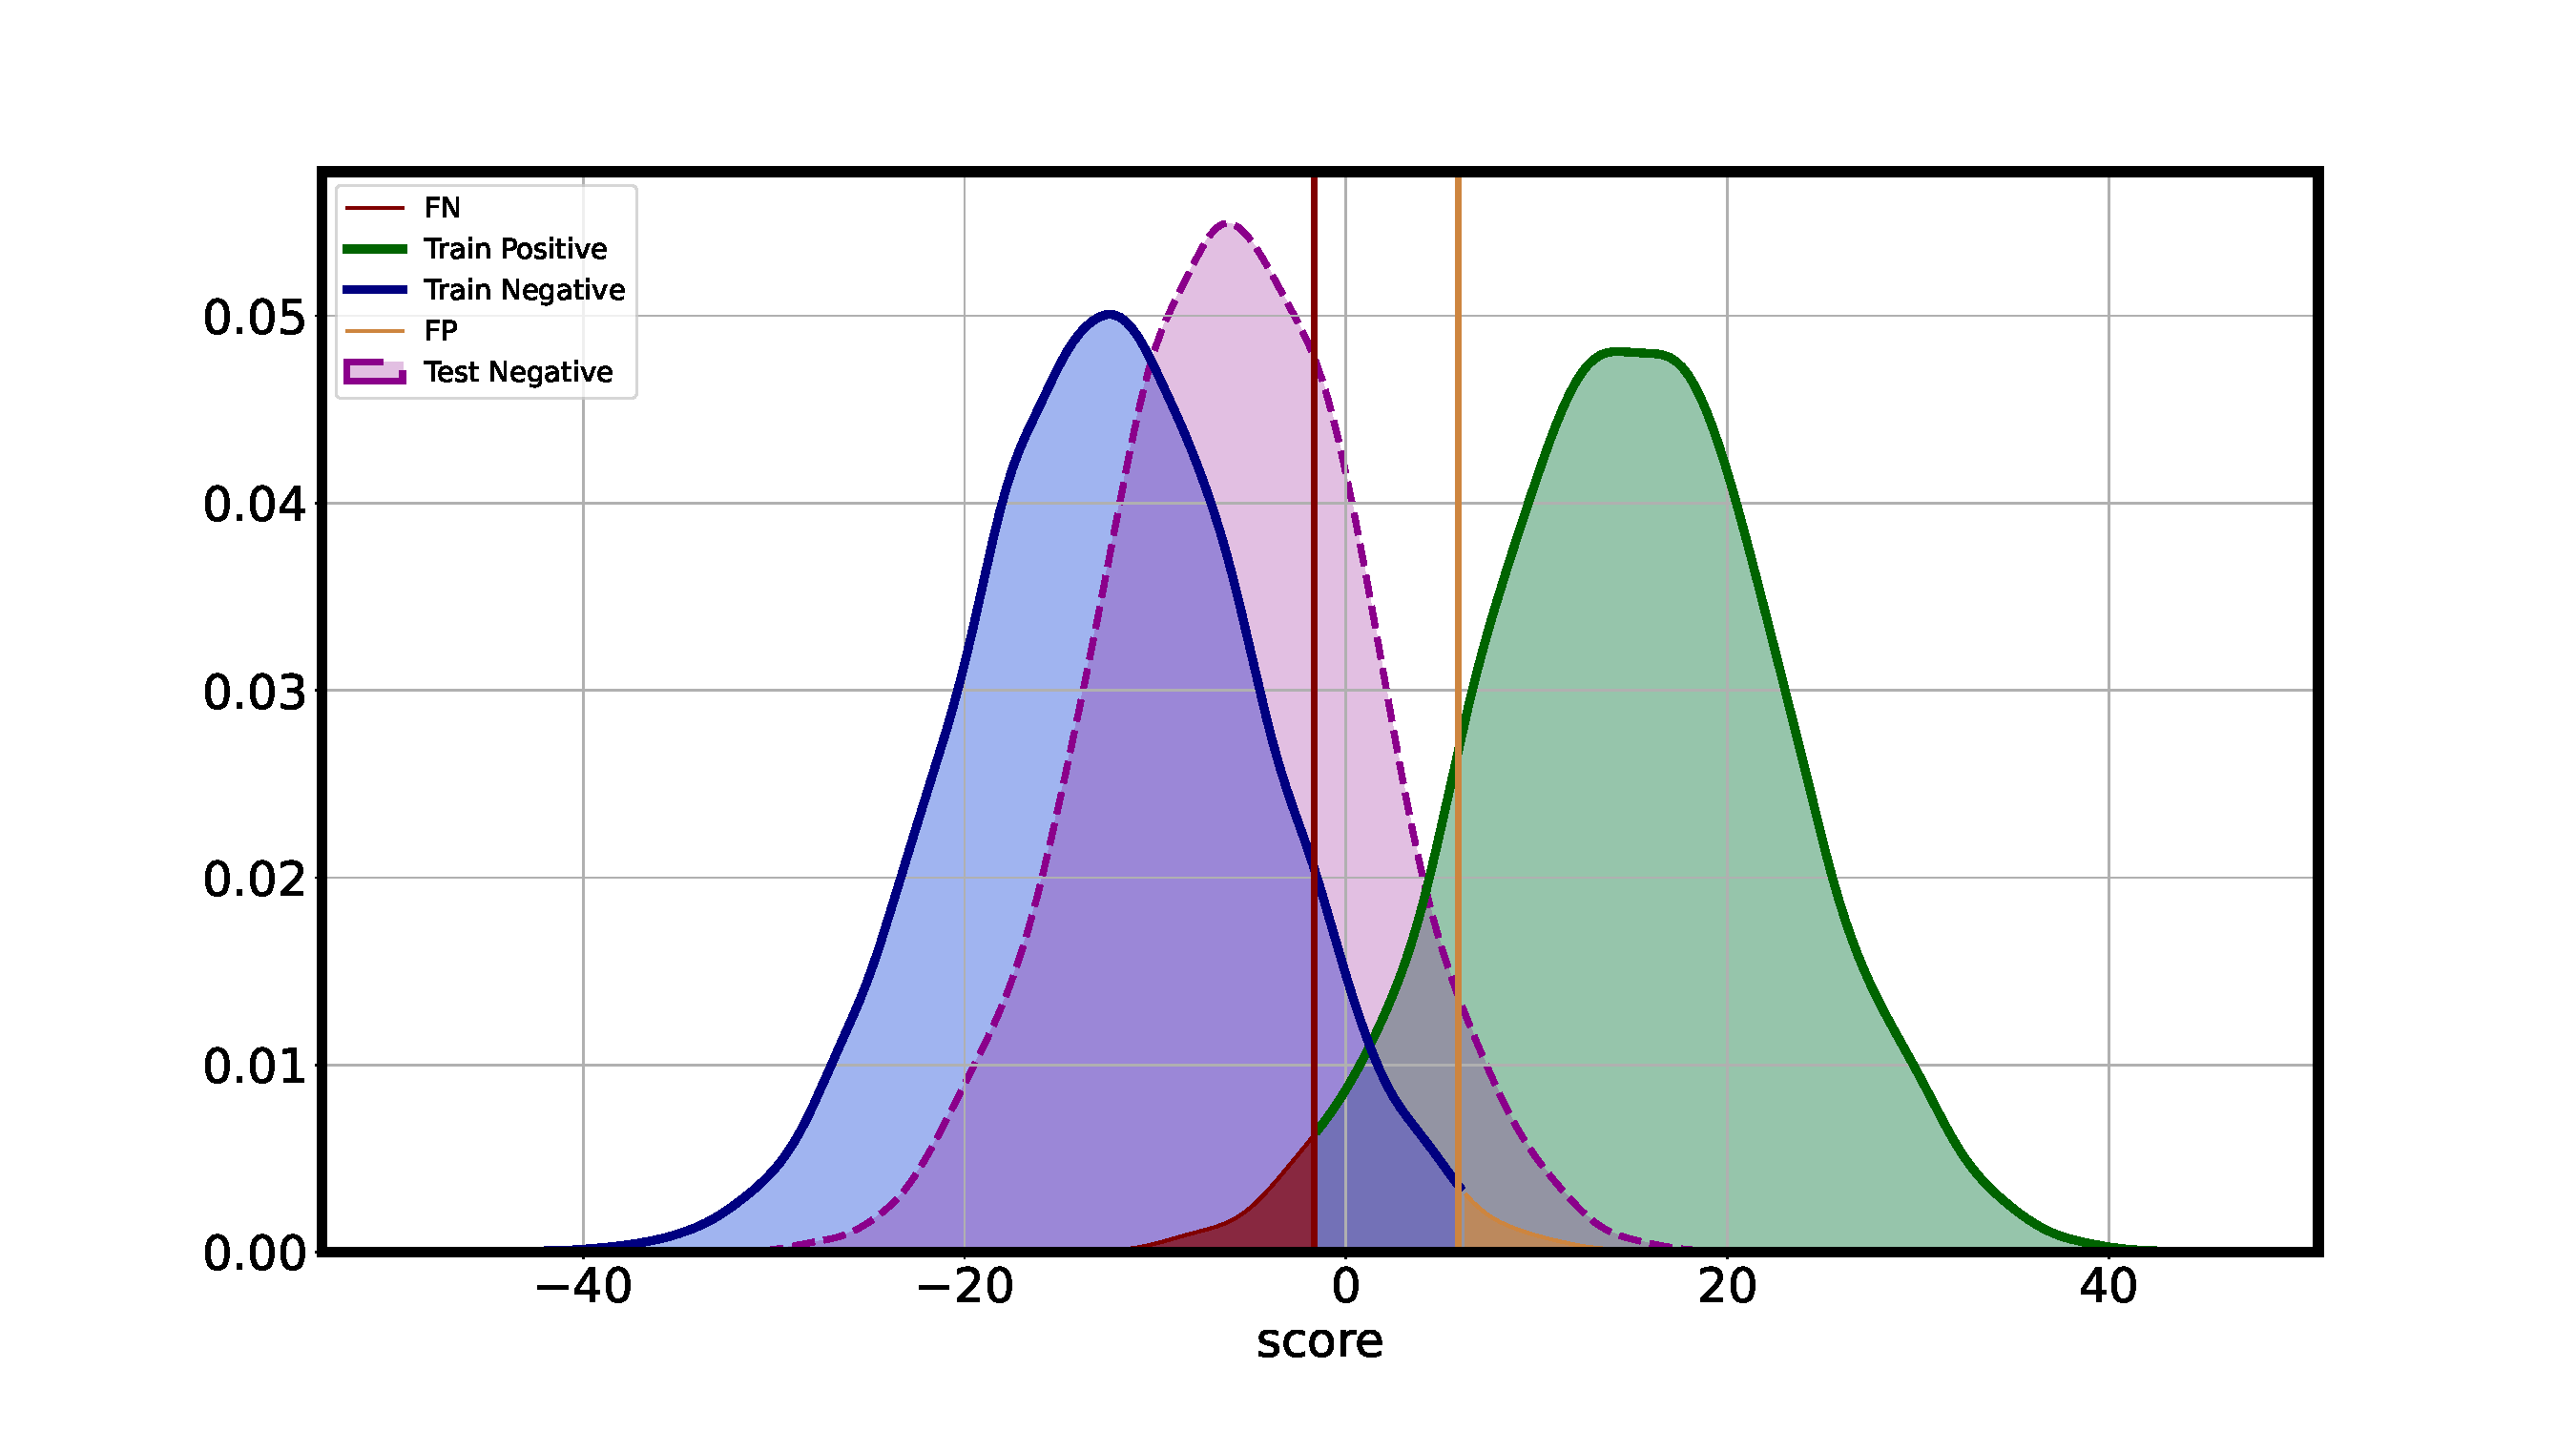
\includegraphics[width=5in]{img/synthetic_overview.pdf}
	\caption{{\bf Error in decision making.} fd}
	\label{fig:illustration}
\end{figure}  




\section{Preliminaries}

Let us suppose that we are given a domain $D$ such as images, text, speech, graphs, time series, tabular data, or the mix of these; furthermore, let $X\subseteq D$ and $T\subseteq D$ denote the training and  the test data samples, respectively. Let $Y_t\in\{0,1\}$ denote the true class label of sample $t\in D$. Let $f:D\rightarrow R$ be appropriately trained binary discriminator (classifier), such as a deep neural network, to predict positive instances, where $R$ denotes the real numbers. Without loss of generality, we assume that higher score $f(t)$ indicates a stronger membership to the positive class. The train null distribution is constructed as $N_0=\{f(t):Y_t = 0,\,\,  t\in X\}$ from the scores of negative instances, the train target distribution is constructed as $N_1=\{f(t): Y_t = 1,\,\,  t\in X\}$ from the scores of positive instances, and the train score distribution is $N_s=\{f(t): t\in X\}$. The true test null $T_0$, true test target $T_1$, and the true score $T_s$ distributions are constructed in a similar way from the test samples with using the true labels. We say that we trust (or accept) a positive prediction of sample $t$ if and only if $f(t)>s_t$ for a given decision threshold  $s_t$ and we make indecision for samples if $f(t) < s_t$. The false discovery proportion (FDP) in a set of samples $K=\{t\in D\}$ at a score threshold $s_t$ is calculated as 
\begin{equation*}
	FDP(s_t,D)=\frac{1+|\{t\in K: Y_t=0,\,f(t)\ge s_t\}|}{|\{t\in K:f(t)\ge s_t\}|},
\end{equation*}
\noindent where $|.|$ denotes set cardinality. We reserve the FDR for the statistical expectation of FDP. FDR control methods aim to calibrate the $s_t$ so that the error rate among trusted predictions is at most level of $\alpha$. % We note that FDR control is related to FSR control in this case, even for $K=2$.%False positives are calculated as $FP=|\{t:Y_t\ne L(t)\}|$
%A label of a sample $t\in D$ is predicted $L(t)=sign(f(t))$. Let $N_0=\{f(t):t\in X,\, Y_t=0\}$,  the null distribution; that is, the set of the discriminative scores of the negative training samples.

% For binary classification problems (K=2), let $f:D\rightarrow R$ be a trained discriminator (classifier), $N_0=\{f(t):t\in X,\, Y_t=0\}$ the train null distribution,  $N_1=\{f(t):t\in X,\, Y_t=1\}$ the train target distribution, and $FDP(s_t)=(1+{|\{t: Y_t=0,\,f(t)\ge s_t\}|)/|\{t:f(t)\ge s_t\}|}$. We say that we trust the positive prediction of sample $t$ if and only if $f(t)>s_t$. We note that the FDR control is not related to FSR control in this case. 

The p-values of the test samples are calculated with using eq. \ref{eq:epv} with respect to $N_0$. The p-value calculation can be time consuming for large $N_0$ sets, in this case, a binned, empirical cumulative distribution function of $N_0$ could be used to calculate the p-values accordingly. The FDR in a set $T$ can be controlled with using the $BH$ protocol at a predetermined $\alpha$ level. For the sake of simplicity, we replace the $\alpha$ with $\alpha/\hat{\pi_0}$ inside BH algorithm, where $\hat{\pi_0}$ is an estimation of $\pi_0$ introduced by Storey \cite{storey2004strong}: $\hat{\pi_0} = (1+\sum_{i=1}^m \mathone\{p_i\ge\lambda\} )/(m(1-\lambda))$ for $\lambda\in (0,1)$. The q-value of a test sample $t\in T$ is defined as $q_t=\min_{z:\le f(t)}FDP( z )$, that is the minimum $\alpha$ level when the sample $t$ would become a trusted prediction. The q-value of a sample would depend on the other samples in the set. The lower the q-value the most trusted a positive prediction is.
%
% THIS IS WITH MULTI CLASS CLASSIFICATION
%Let us suppose that we are given a domain $D$ such as images, text, speech, graphs, time series, tabular data, or the mix of these; furthermore, let $X\subseteq D$ and $T\subseteq D$ denote the training and  the test data samples, respectively. Let $Y_t\in\{0,\dots, K-1\}$ denote the true class label of sample $t\in D$. Let $f_k:D\rightarrow R$ be appropriately trained discriminators (classifiers), such as a deep neural network, to indicate class memberships ($k=0,1,\dots,K-1$), where $R$ denotes the real values. Without loss of generality, we assume that higher score $f_k(t)$ indicates a stronger membership to class $k$. Then, let $f(t)= \max_k\{f_k(t) \}$ and $L(t)=\text{argmax}_k\{f_k(t)\}$ be the predicted class label for $t\in D$. The train null distribution is constructed as $N_0=\{f(t): L(t) \ne Y_t,\,\,  t\in X\}$ from the scores of incorrect classifications, the train target distribution is constructed as $N_1=\{f(t): L(t) = Y_t,\,\,  t\in X\}$ from the scores of correct classifications. The true test null and true test target distributions are constructed in a similar way from the test samples with using the true labels, respectively.  We say that, we trust a prediction $L(t)$ for a sample $t$  if $f(t)\ge s_t$ for a decision threshold $s_t$, and we make indecision for samples if $f(t) < s_t$. The false discovery proportion (FDP) in a set of samples $\{t\in D\}$ at a score threshold $s_t$ is calculated as 
%\begin{equation}
%	FDP(s_t)=\frac{1+|\{t: Y_t\ne L(t),\,f(t)\ge s_t\}|}{|\{t:f(t)\ge s_t\}|},
%\end{equation}
%\noindent where $|.|$ denotes set cardinality. We reserve the FDR for the statistical expectation of FDP. FDR control aims to calibrate the $s_t$ so that the error rate among trusted predictions is at level of $\alpha$. We note that FDR control is related to FSR control in this case, even for $K=2$.%False positives are calculated as $FP=|\{t:Y_t\ne L(t)\}|$
%%A label of a sample $t\in D$ is predicted $L(t)=sign(f(t))$. Let $N_0=\{f(t):t\in X,\, Y_t=0\}$,  the null distribution; that is, the set of the discriminative scores of the negative training samples.
%
%For binary classification problems (K=2), let $f:D\rightarrow R$ be a trained discriminator (classifier), $N_0=\{f(t):t\in X,\, Y_t=0\}$ the train null distribution,  $N_1=\{f(t):t\in X,\, Y_t=1\}$ the train target distribution, and $FDP(s_t)=(1+{|\{t: Y_t=0,\,f(t)\ge s_t\}|)/|\{t:f(t)\ge s_t\}|}$. We say that we trust the positive prediction of sample $t$ if and only if $f(t)>s_t$. We note that the FDR control is not related to FSR control in this case. 
%
%The p-values of the test samples are calculated with using eq. \ref{eq:epv} with respect to $N_0$. The p-value calculation can be time consuming for large $N_0$ sets, in this case, a binned, empirical cumulative distribution function of $N_0$ could be used to calculate the p-values accordingly. The FDR in a set $T$ can be controlled with using the $BH$ protocol at a predetermined $\alpha$ level. For the sake of simplicity, we replace the $\alpha$ with $\alpha/\hat{\pi_0}$ inside BH algorithm, where $\hat{\pi_0}$ is an estimation of $\pi_0$ introduced by Storey \cite{storey2004strong}: $\hat{\pi_0} = (1+\sum_{i=1}^m \mathone\{p_i\ge\lambda\} )/(m(1-\lambda))$ for $\lambda\in (0,1)$. The q-value of a test sample $t\in T$ is defined as $q_t=\min_{z:\le f(t)}FDP( z )$, that is the minimum $\alpha$ level when the sample $t$ would become a trusted prediction. The q-value of a sample would depend on the other samples in the set. The lower the q-value the most trusted the prediction is.

%\paragraph{Example 1.} For demonstration, we trained a two-layer convolutional neural network containing 8 kernels with size of $3\times3$ at each layers, respectively, to predict the hand-written digits of the MNIST samples. The MNIST dataset contains 60K training and 10K test images of 28x28 pixels in 10 classes. There is no shift in the test set. The accuracy of the trained model is 0.975. The score distributions 

\paragraph{Example 	 1.} \label{ex:vanilla} We used the NIST dataset for demonstration. The MNIST dataset contains 60K training and 10K test images of 28x28 grey-scaled pixels in 10 classes. There is no shift between the train and test data. We trained a convolutional neural network to classify the digit '1' as target (positive) against all the other digits (negative) (binary classification). Our ConvNet model contained two convolutional layers consisting of 8 kernels with size of $3\times3$ at each layers, and it was trained with Adam optimizer with a learning rate of 0.01 for three epochs. Our trained model achieved a 99\% accuracy on the test set. The relevant results are presented in Figure \ref{fig:binary}. The Figure \ref{fig:binary}A shows the train and test null and target distributions. This plot indicates that there is no shift between the train and test distributions. The Figure \ref{fig:binary}B shows a QQ plot of the empirical p-values calculated with Eq. [1] using $N_0$ against the theoretical uniform distributions. A diagonal line shows that the empirical p-values calculated are valid. We also performed the Fisher's combined test to check whether the empirical p-values are uniformly distribution. The test produces a p-value of 0.934 indicating uniformly distributed empirical p-values. Therefore, BH can control the FDR accurately at various levels (q-values). This is shown in \ref{fig:binary}C, where the true (black solid line) and the accepted predictions (green dashed line) are closely overlap at various FDR levels (q-values). As a comparison, we also evaluated the LTT method \cite{angelopoulos2021learn} (dashed blue line), and results confirm that LTT is also an accurate method to control the FDR in the lack of data distribution shift. Finally, the Figure \ref{fig:binary}D shows the deviation of the estimated FDRs from the true FDRs is small.



\begin{figure}
	\centering
	\begin{tabular}{cccc}
		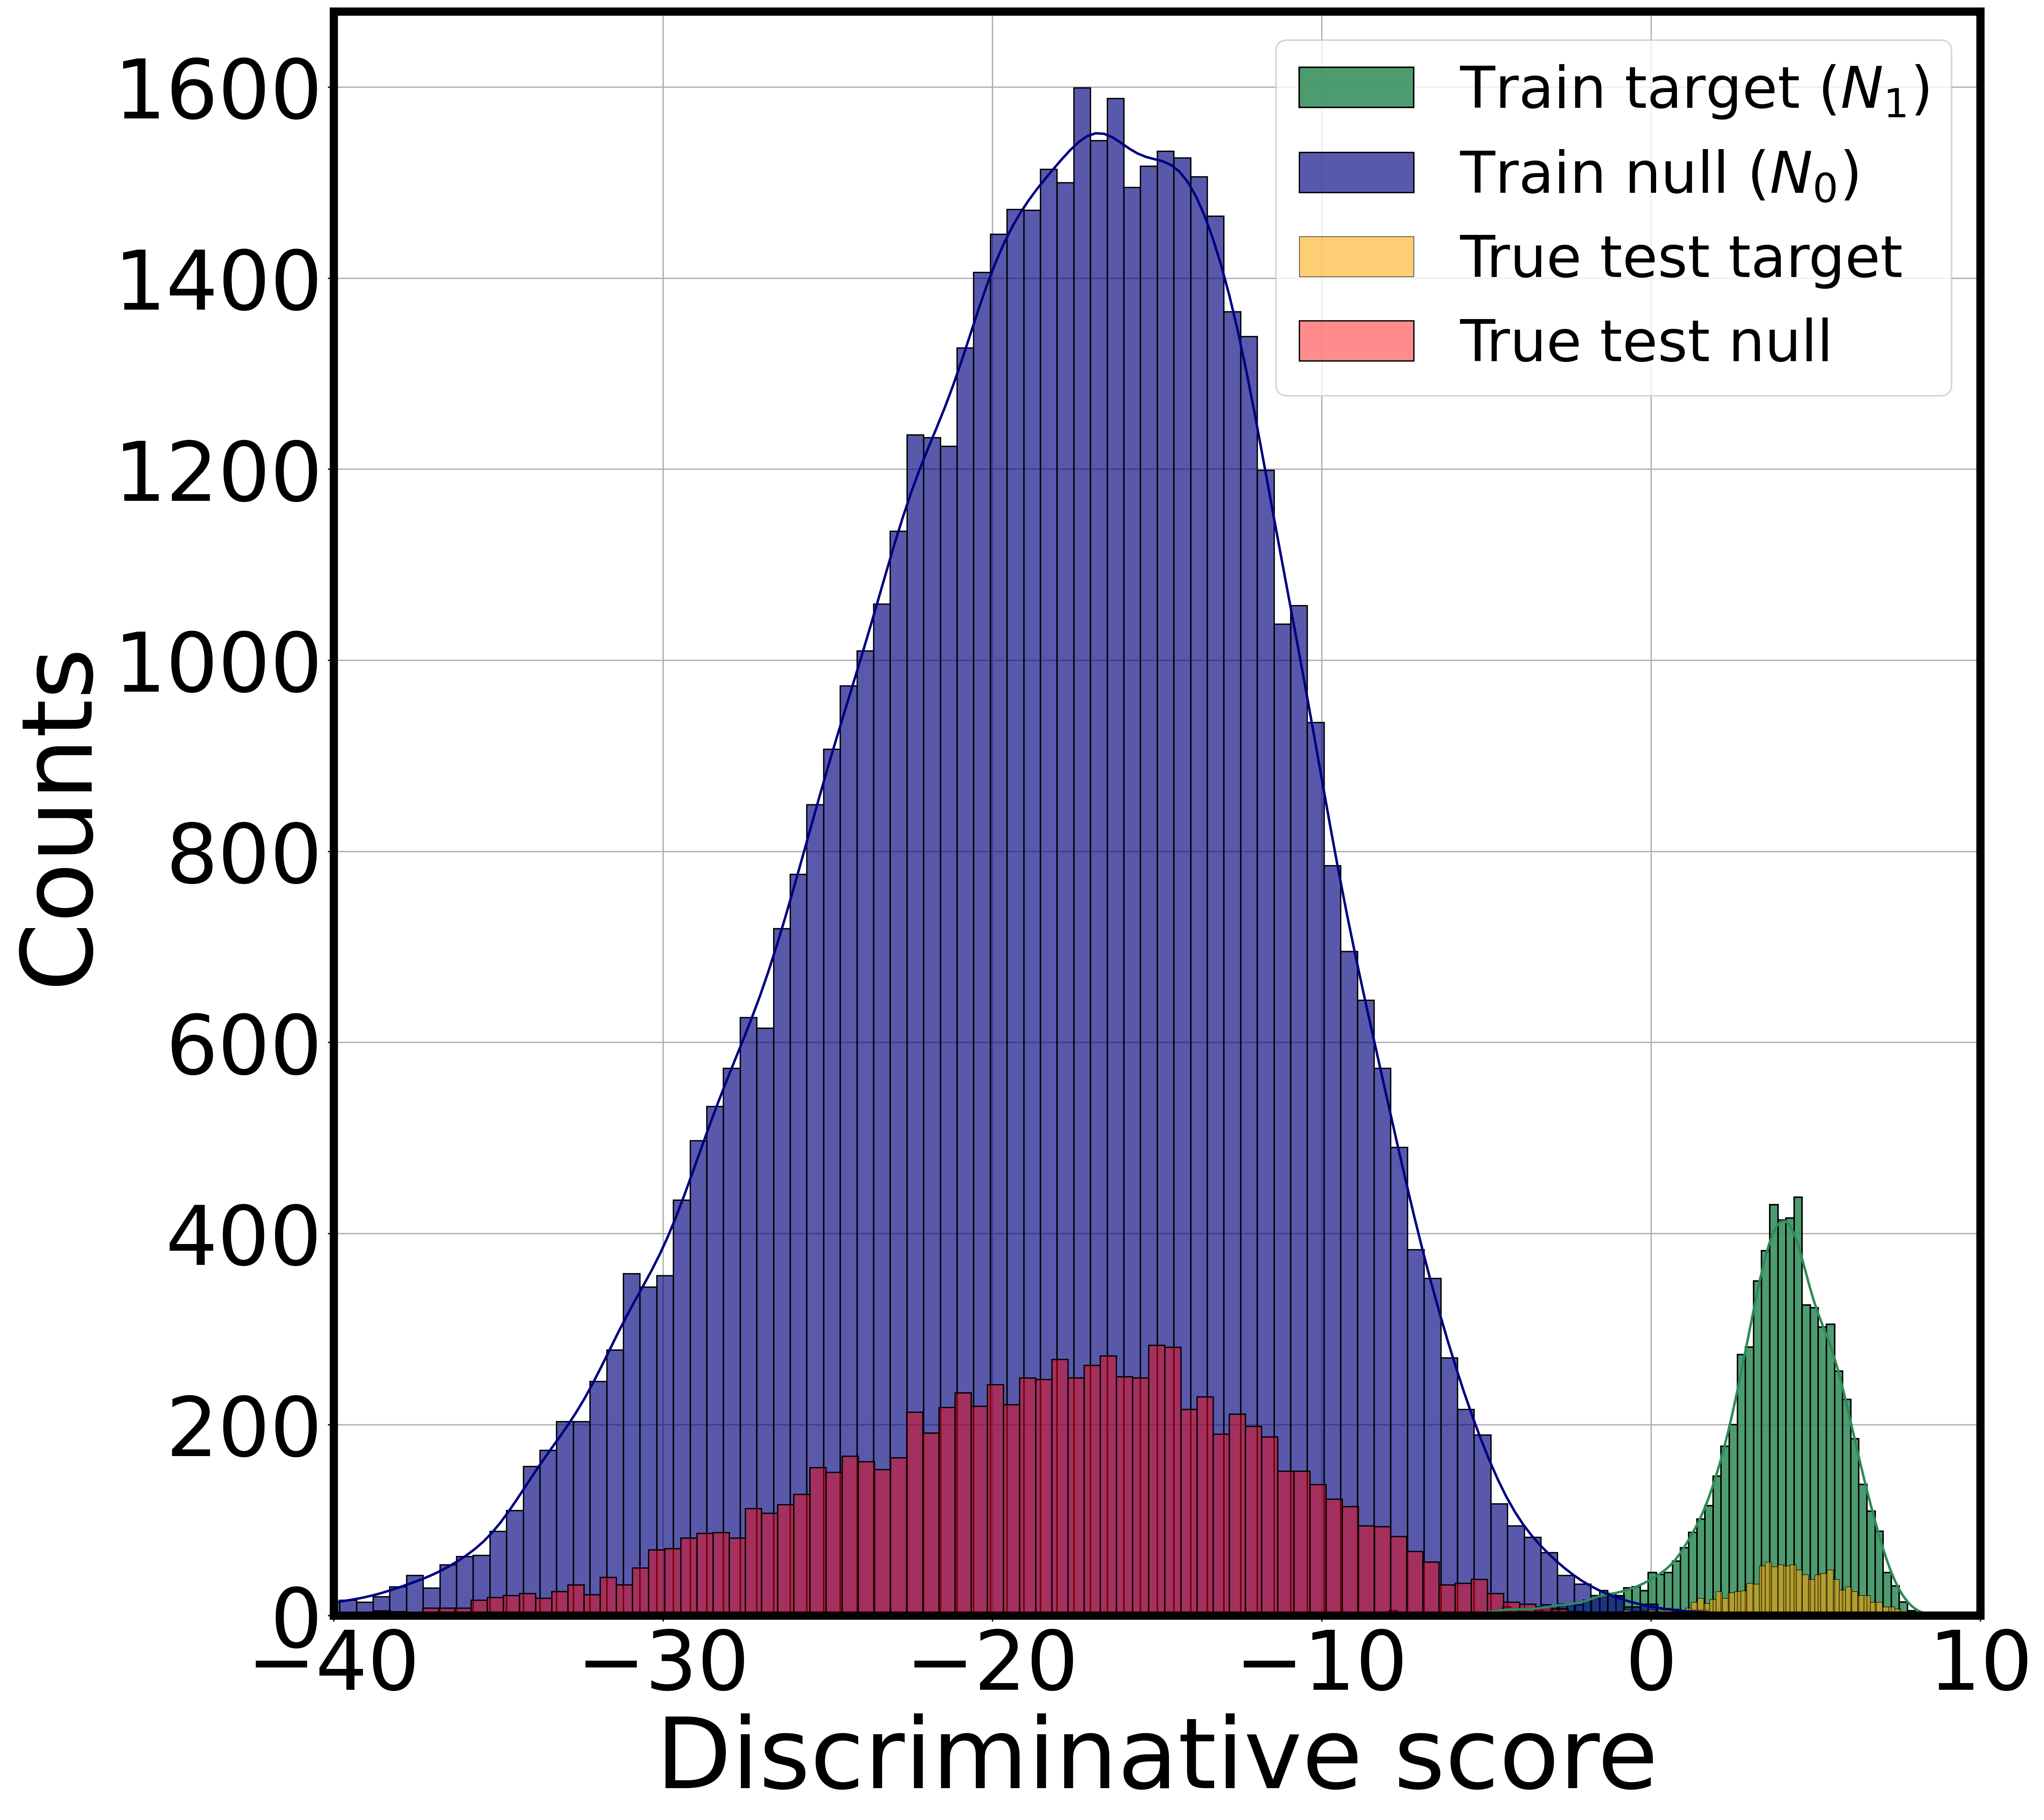
\includegraphics[width=1.7in]{img/cls_overview.png}&
		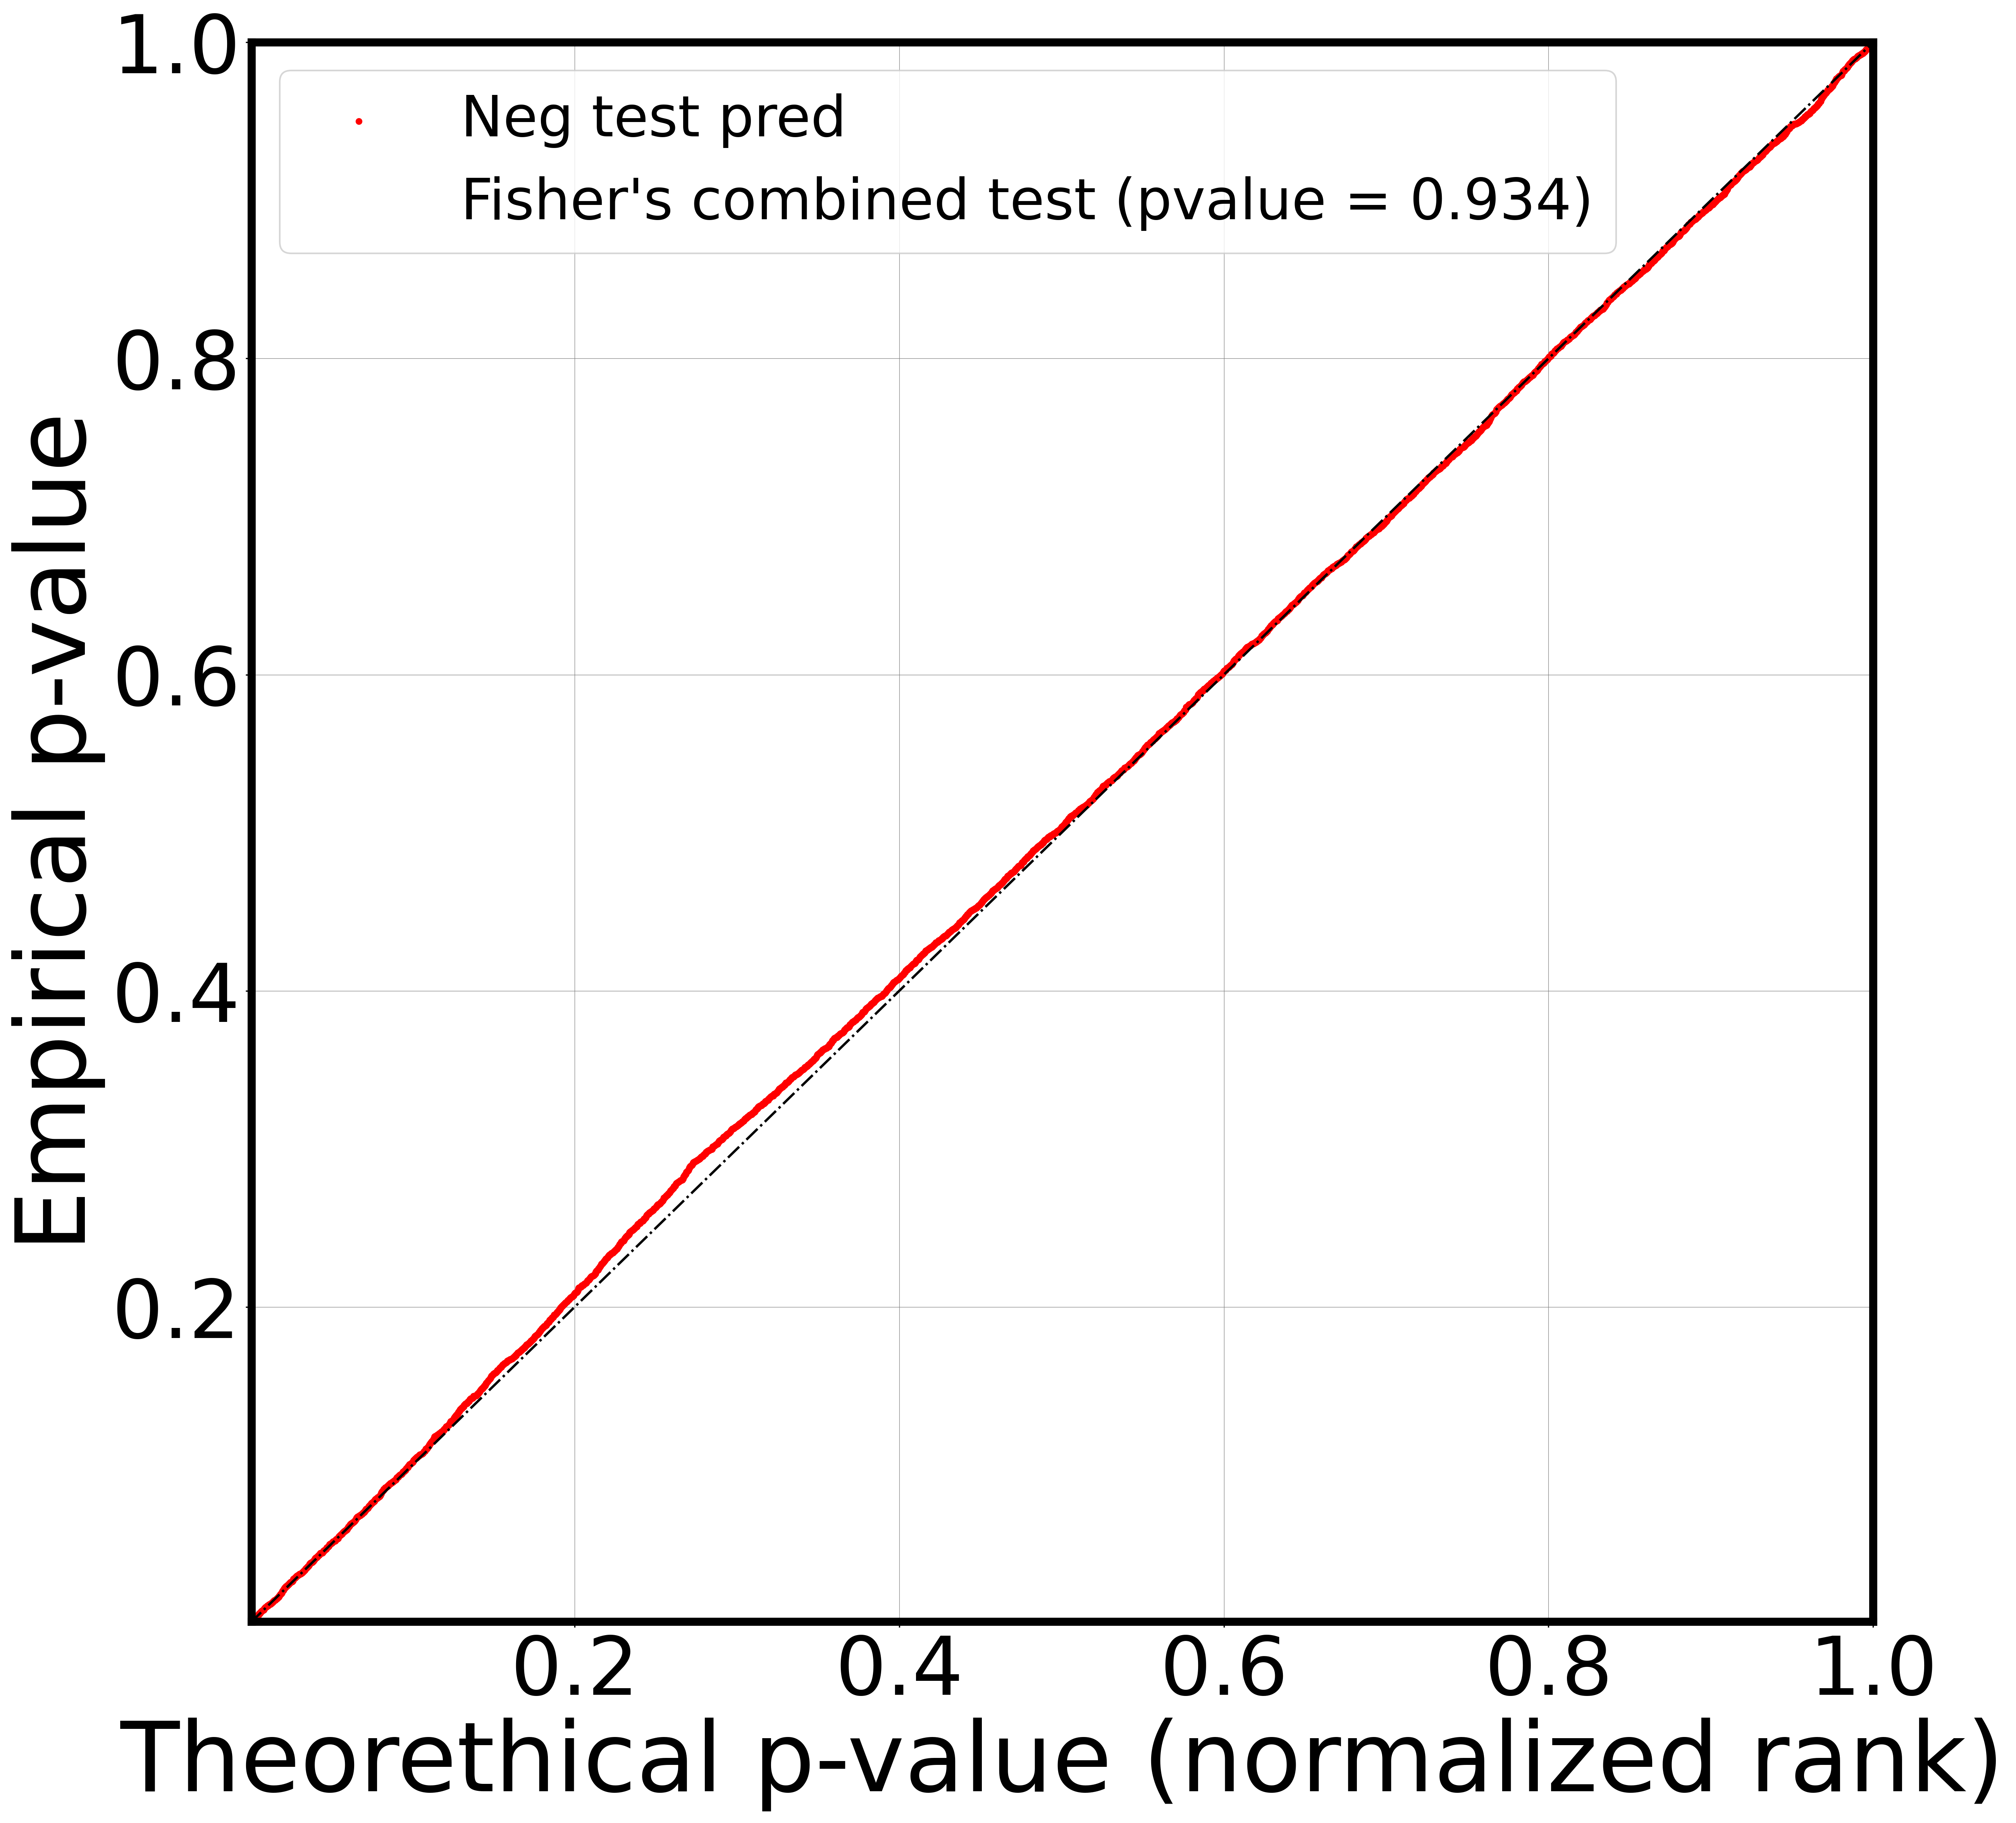
\includegraphics[width=1.7in]{img/cnn_QQ_classical_lin.png} &
		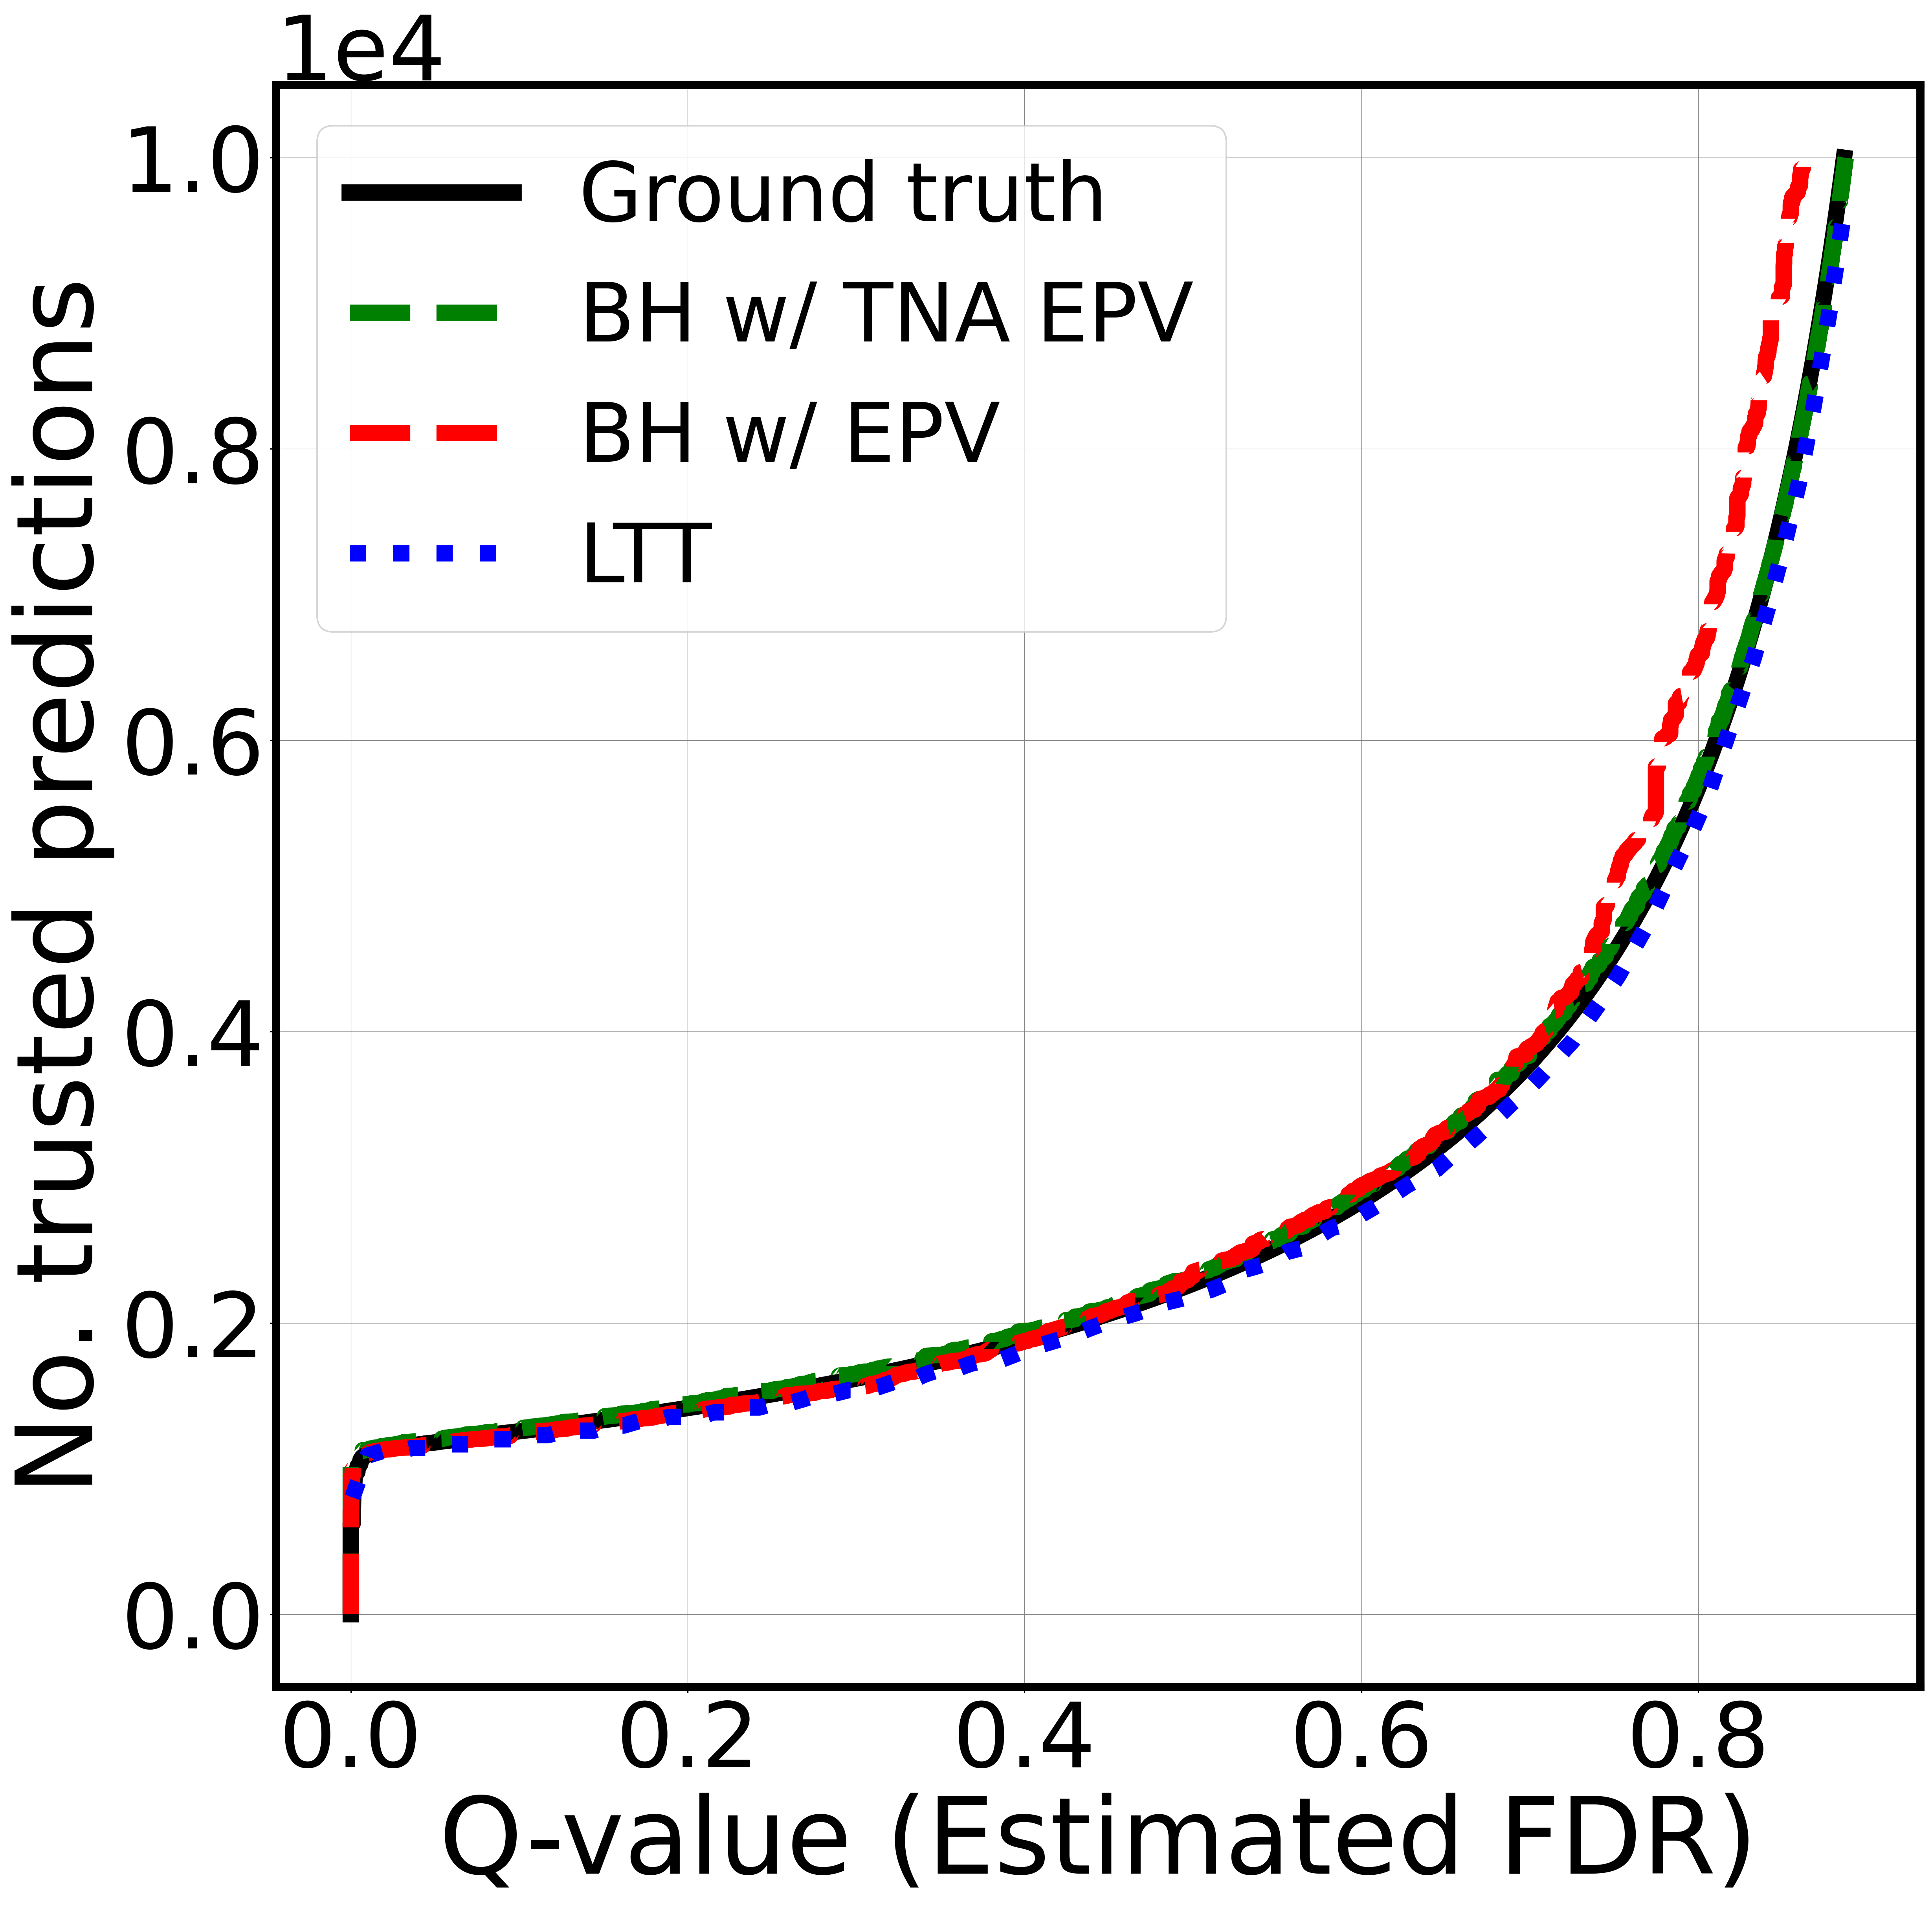
\includegraphics[width=1.7in]{img/cnn_classical_fdr_control.png} &
		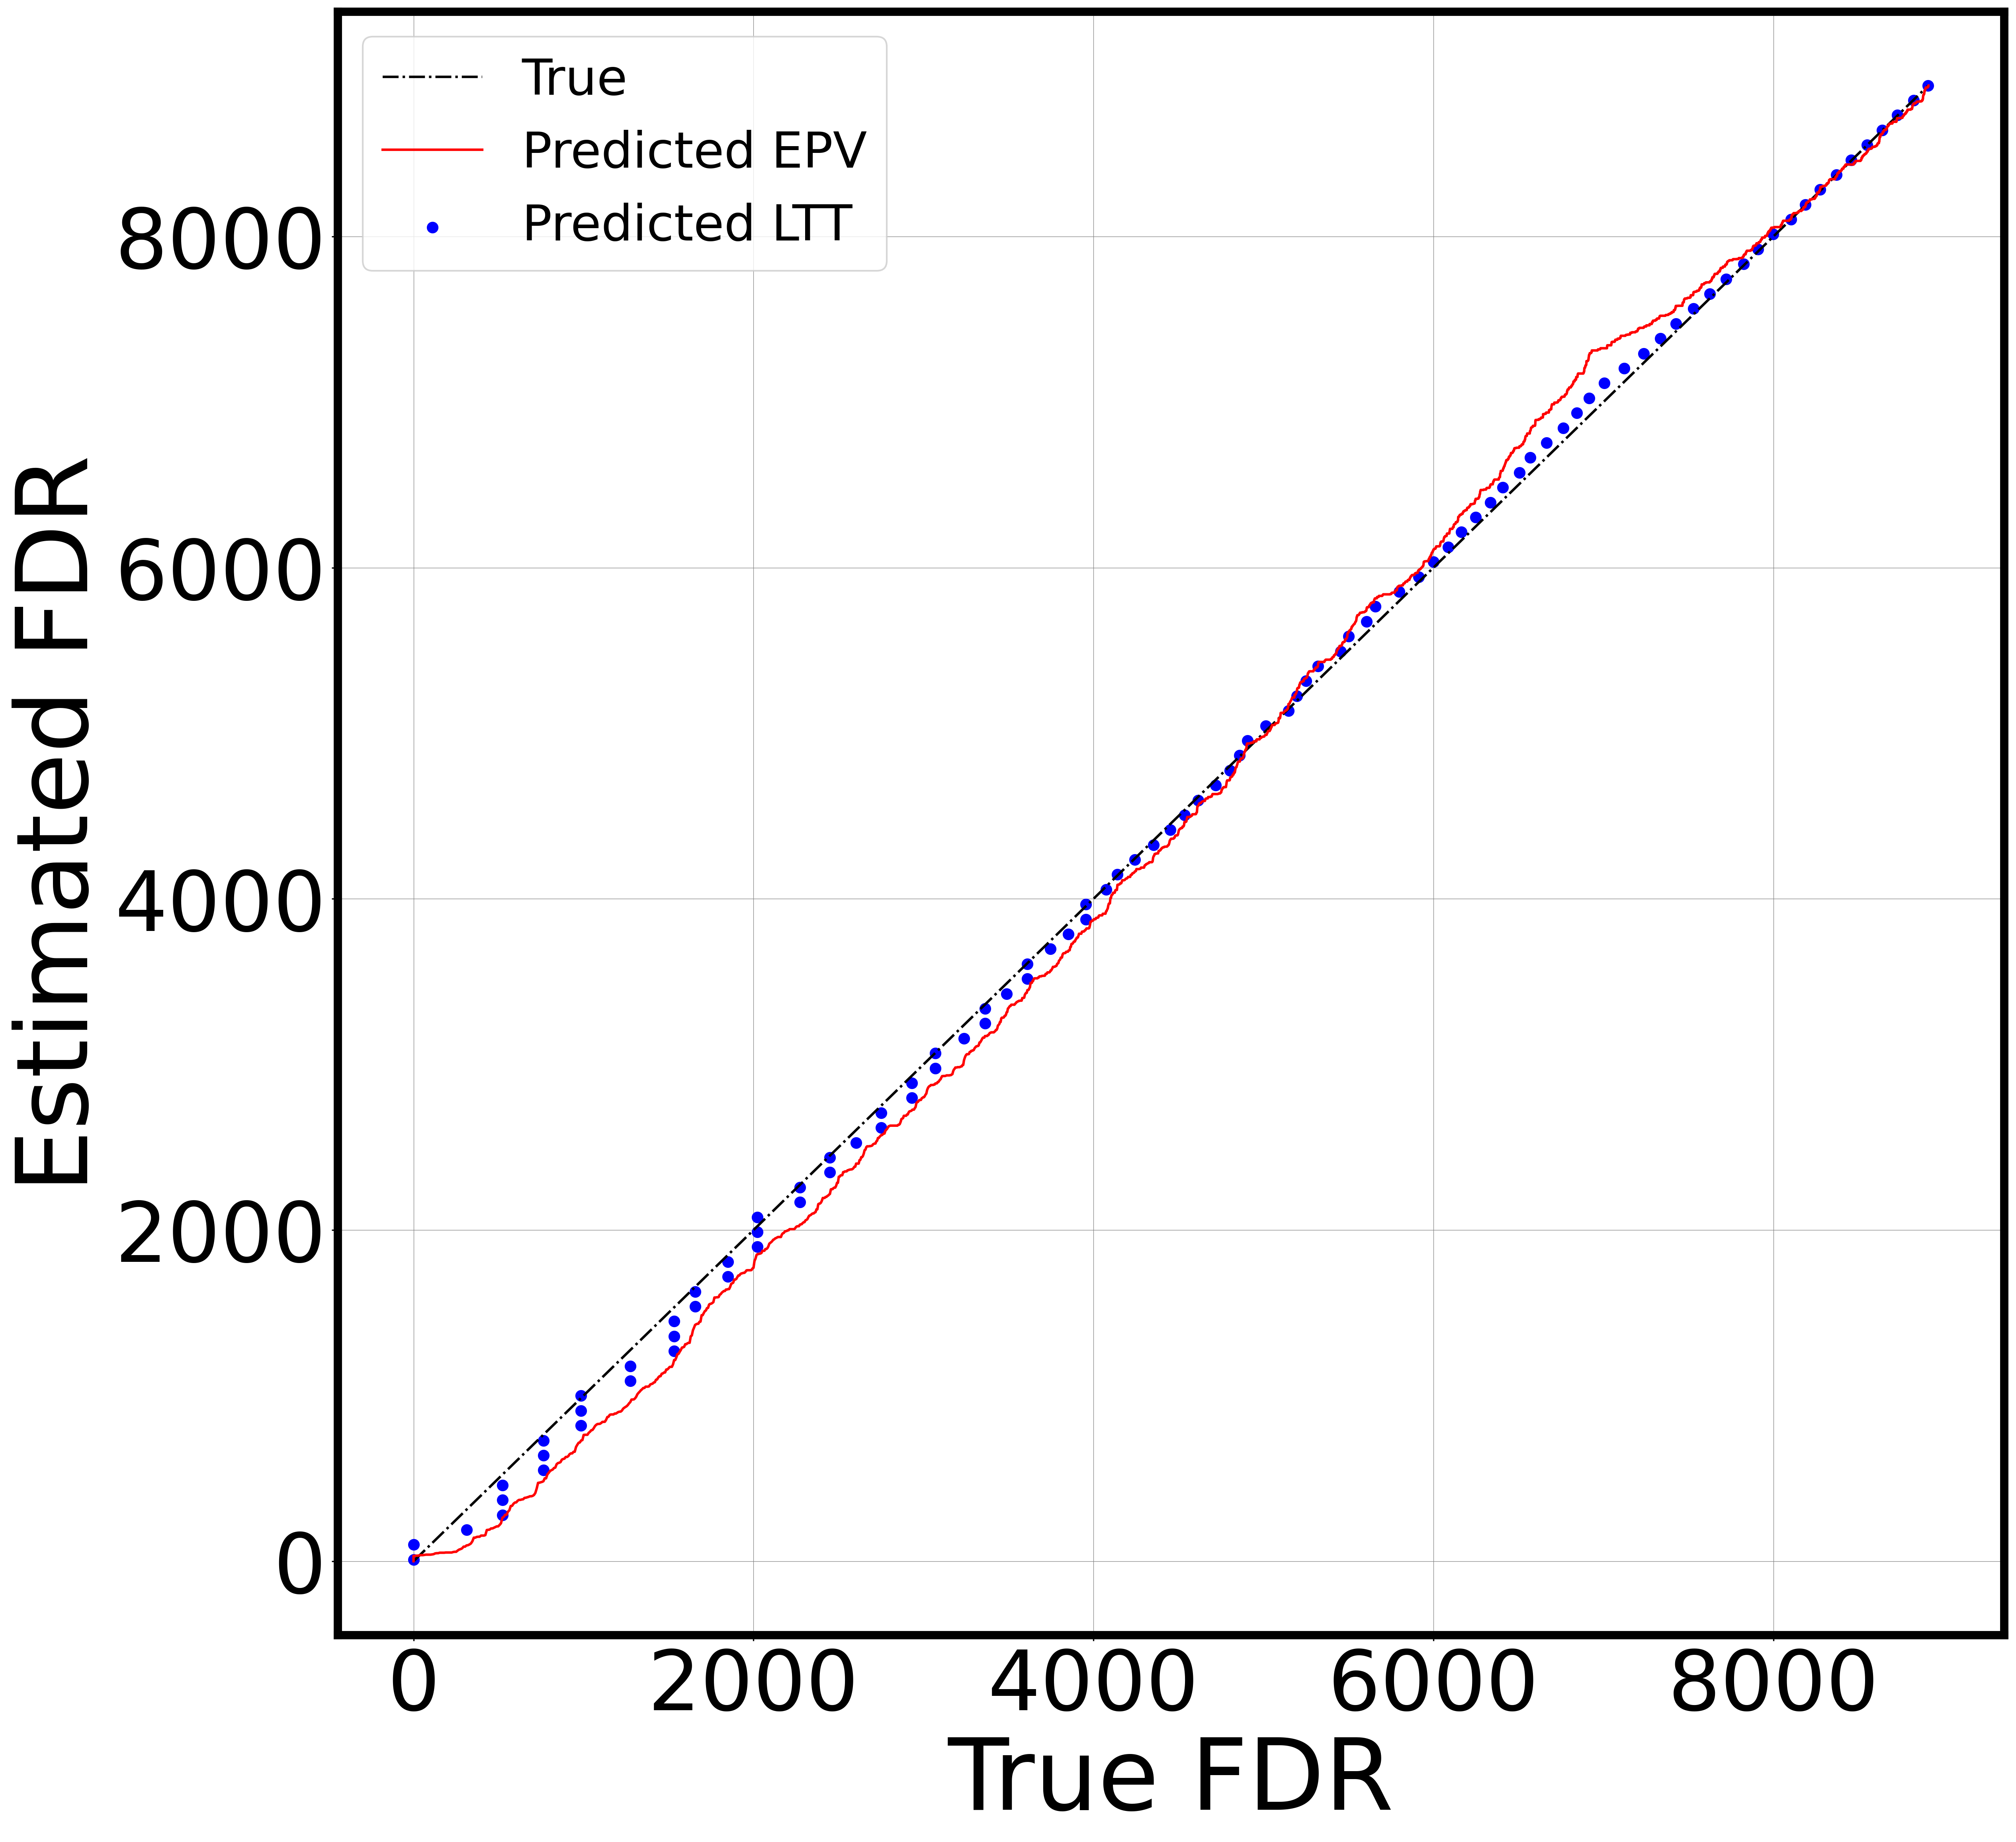
\includegraphics[width=1.7in]{img/cnn_FDRQQ_classical.png} \\
			
		A & B & C & D \\

	\end{tabular}
	\caption{{\bf FDR control in MNIST predictions with empirical p-values. } (A) The discriminative score distributions. \todo{AB}{The legends should be: Train null ($N_0$), Train target ($N_1$), Test null ($T_0$), Test target ($T_1$).}.(B) The QQ plot of the empirical p-values of the test samples against the theoretical uniform distribution. (C) The number of true and accepted positive predictions by LTT and BH at various FDR levels (Q-values).  (D)  (D) Deviation of the estimated FDR from the actual FDR obtained with (i) BH with EPV (red line), and (ii) LTT (blue line). \todo{AB}{The legends should be: 1. BH with EPV, 2. LTT} }
	\label{fig:binary}
\end{figure}
 

%
%\section{Test Null Approximation}
%When the train null distribution $N_0$ is different from the null distribution $T_0$ of the test instances, then the empirical p-values will not be uniformly distributed resulting in liberal or conservative bias in  FDR estimation.
%
%
%The approximation of the null distribution in the distribution of the test scores is performed through the following steps.
%
%
%\begin{enumerate}%[label=\arabic*.]
%    \item The train null distribution $N_0$ is adjusted to the distribution of the negative test predictions. Let $\mu_{T_0}$ and $\sigma_{T_0}$ denote the mean and the standard deviation of $T_0$. The train null is adjusted via $\hat{N_0} = \frac{N_0-\nu_{T_0}}{\sigma_{T_0}+\epsilon}$, where $\epsilon$ is a small numerical regularization parameter.
%    
%    \item The proportions of the nulls among the test instances is estimated $\hat{\pi_0}=N_t/(N_t+P_t)$, where $N$ and $P$ denote the  number of negative and positive test predictions, respectively. We note that, this ratio can be very different from the one of the train data. 
%    
%    \item A histograms of $\hat{N_0}$ and $T$ is constructed with the same binning. The histograms are denoted with $H_{N_0}$ and $H_T$, and $H[i]$ denotes the counts in bin $i$. In our experiments the bin width was set to 1.0 and it worked fine.
%    
%    \item Finally, we construct the histogram of the test null $H_{T_0}$ via $H_{T_0}[i]= H_T[i]*c_i*\hat{\pi_0}$, where $c_i=P[i]/N[i]$, i.e. the fraction of the negatives among the train data in the ith bin, in the histogram.
%    
%\end{enumerate}
%
%This final histogram $H_{T_0}$ is used to calculate the empirical p-values for each test instances. 
%    

\section{Test null adjustment (TNA) method}
When the train null distribution $N_0$ is different from the null distribution $T_0$ of the test instances, then the empirical p-values will not be uniformly distributed and the BH procedure results in liberal or conservative bias in FDR estimation. In the following steps, we describe our methods how to adjust the test scores so that the test null distribution $T_0$ approximates the train null distribution $N_0$.

\begin{enumerate}%[label=\arabic*.]
	\itemsep-3pt  		
	\item Get the histograms of $N_0$, $N$, and $T$ distributions with identical bin borders and denote them as $H_0$, $H_N$, and $H_T$, respectively. $H_x[i]$ denotes the counts in bin $i$.  In our experiments the bin width was set to 1.0 and it worked fine. \textbf{No, the bin width was either linear, with 100 bins being split across train distribution or at log scale,also 100 bins}
	
	\item Let $\pi_N$ be the proportions of negative samples in the training data, and $\pi_T$ be the proportions of the negative predictions among all test predictions, and let $\tau=\pi_T/\pi_N$. 
	
	\item Let us create a new histogram, which will be an approximation of the test null distribution, $\hat{T_0}[i]=T[i]\cdot c_i\cdot \tau$, where $c_i=H_0[i]/H_N[i]$ is the proportion of negative training samples in bin $i$.
	
	\item Let $\mu_{N_0}$, $\sigma_{N_0}$, $\mu_{\hat{T_0}}$, and $\sigma_{\hat{T_0}}$ are the mean and std of the $N_0$ and the $\hat{T_0}$ distributions, respectively. 
	
	\item Adjust the test scores $\hat{t_s} = (t_s-\mu_{\hat{T_0}})/\sigma_{\hat{T_0}} \cdot \sigma_{\hat{N_0}} + \mu_{N_0}$ for approximated as negative test instances $t$ of distribution $\hat{T_0}$.
\end{enumerate}


	Finally, calculate the empirical p-values for each $\hat{t_s}$ with the $N_0$ distribution, estimate  $\hat{\pi_0}$ for the test instances with the Storey method with $\beta= ..$, and run BH procedure to control the FDR at a desired level. \todo{AB}{Please draw a sketch to illustrate the TBA method.}
	
	
	
%	
%	1. train 0, as fixed, named N0. calculate mu and sigma for N0. 
%	2. take negative test predictions. calculate mu and sigma for test negative.
%	3. move all test negative to train 0. This is not critical. 
%	4. what do you do with test positive? can we also move test postivie with 
%    4a . I think, should be done: test_instance_score: t_i := (t_i-mu)/sigma. skip this.
%% Andrey says, steps 1-4 are not important.
%    5. histograming train scores and test scores with identical bin (borders).
%    6. calculate proportion of train negatives among train scores in each bin.
%    7. estimate pi_0, based on the number of test positive and test negataive predictions. 
%    8. bins on positive side of the x-axis: 
%    9. here you do some scaling. 
%    10. bin i. 
%    11. calculate again mu and sigma of new test negative,  
%    12. adjust test negative to N0,
%    13. calculate p-values with the adjusted test negative? Use Storey method to estimate lambda, and estimate the pi_0.
%    14. use BH to control FDR. 
%	
	
%	
%	\item The train null distribution $N_0$ is adjusted to the distribution of the negative test predictions. Let $\mu_{T_0}$ and $\sigma_{T_0}$ denote the mean and the standard deviation of $T_0$. The train null is adjusted via $\hat{N_0} = \frac{N_0-\nu_{T_0}}{\sigma_{T_0}+\epsilon}$, where $\epsilon$ is a small numerical regularization parameter.
%	
%	\item The proportions of the nulls among the test instances is estimated $\hat{\pi_0}=N_t/(N_t+P_t)$, where $N$ and $P$ denote the  number of negative and positive test predictions, respectively. We note that, this ratio can be very different from the one of the train data. 
%	
%	\item A histograms of $\hat{N_0}$ and $T$ is constructed with the same binning. The histograms are denoted with $H_{N_0}$ and $H_T$, and $H[i]$ denotes the counts in bin $i$. In our experiments the bin width was set to 1.0 and it worked fine.
%	
%	\item Finally, we construct the histogram of the test null $H_{T_0}$ via $H_{T_0}[i]= H_T[i]*c_i*\hat{\pi_0}$, where $c_i=P[i]/N[i]$, i.e. the fraction of the negatives among the train data in the ith bin, in the histogram.


\begin{figure}[h!]
	\centering
	\begin{tabular}{cccc}
		\multicolumn{4}{l}{\bf (i) Data distribution shift:}\\
		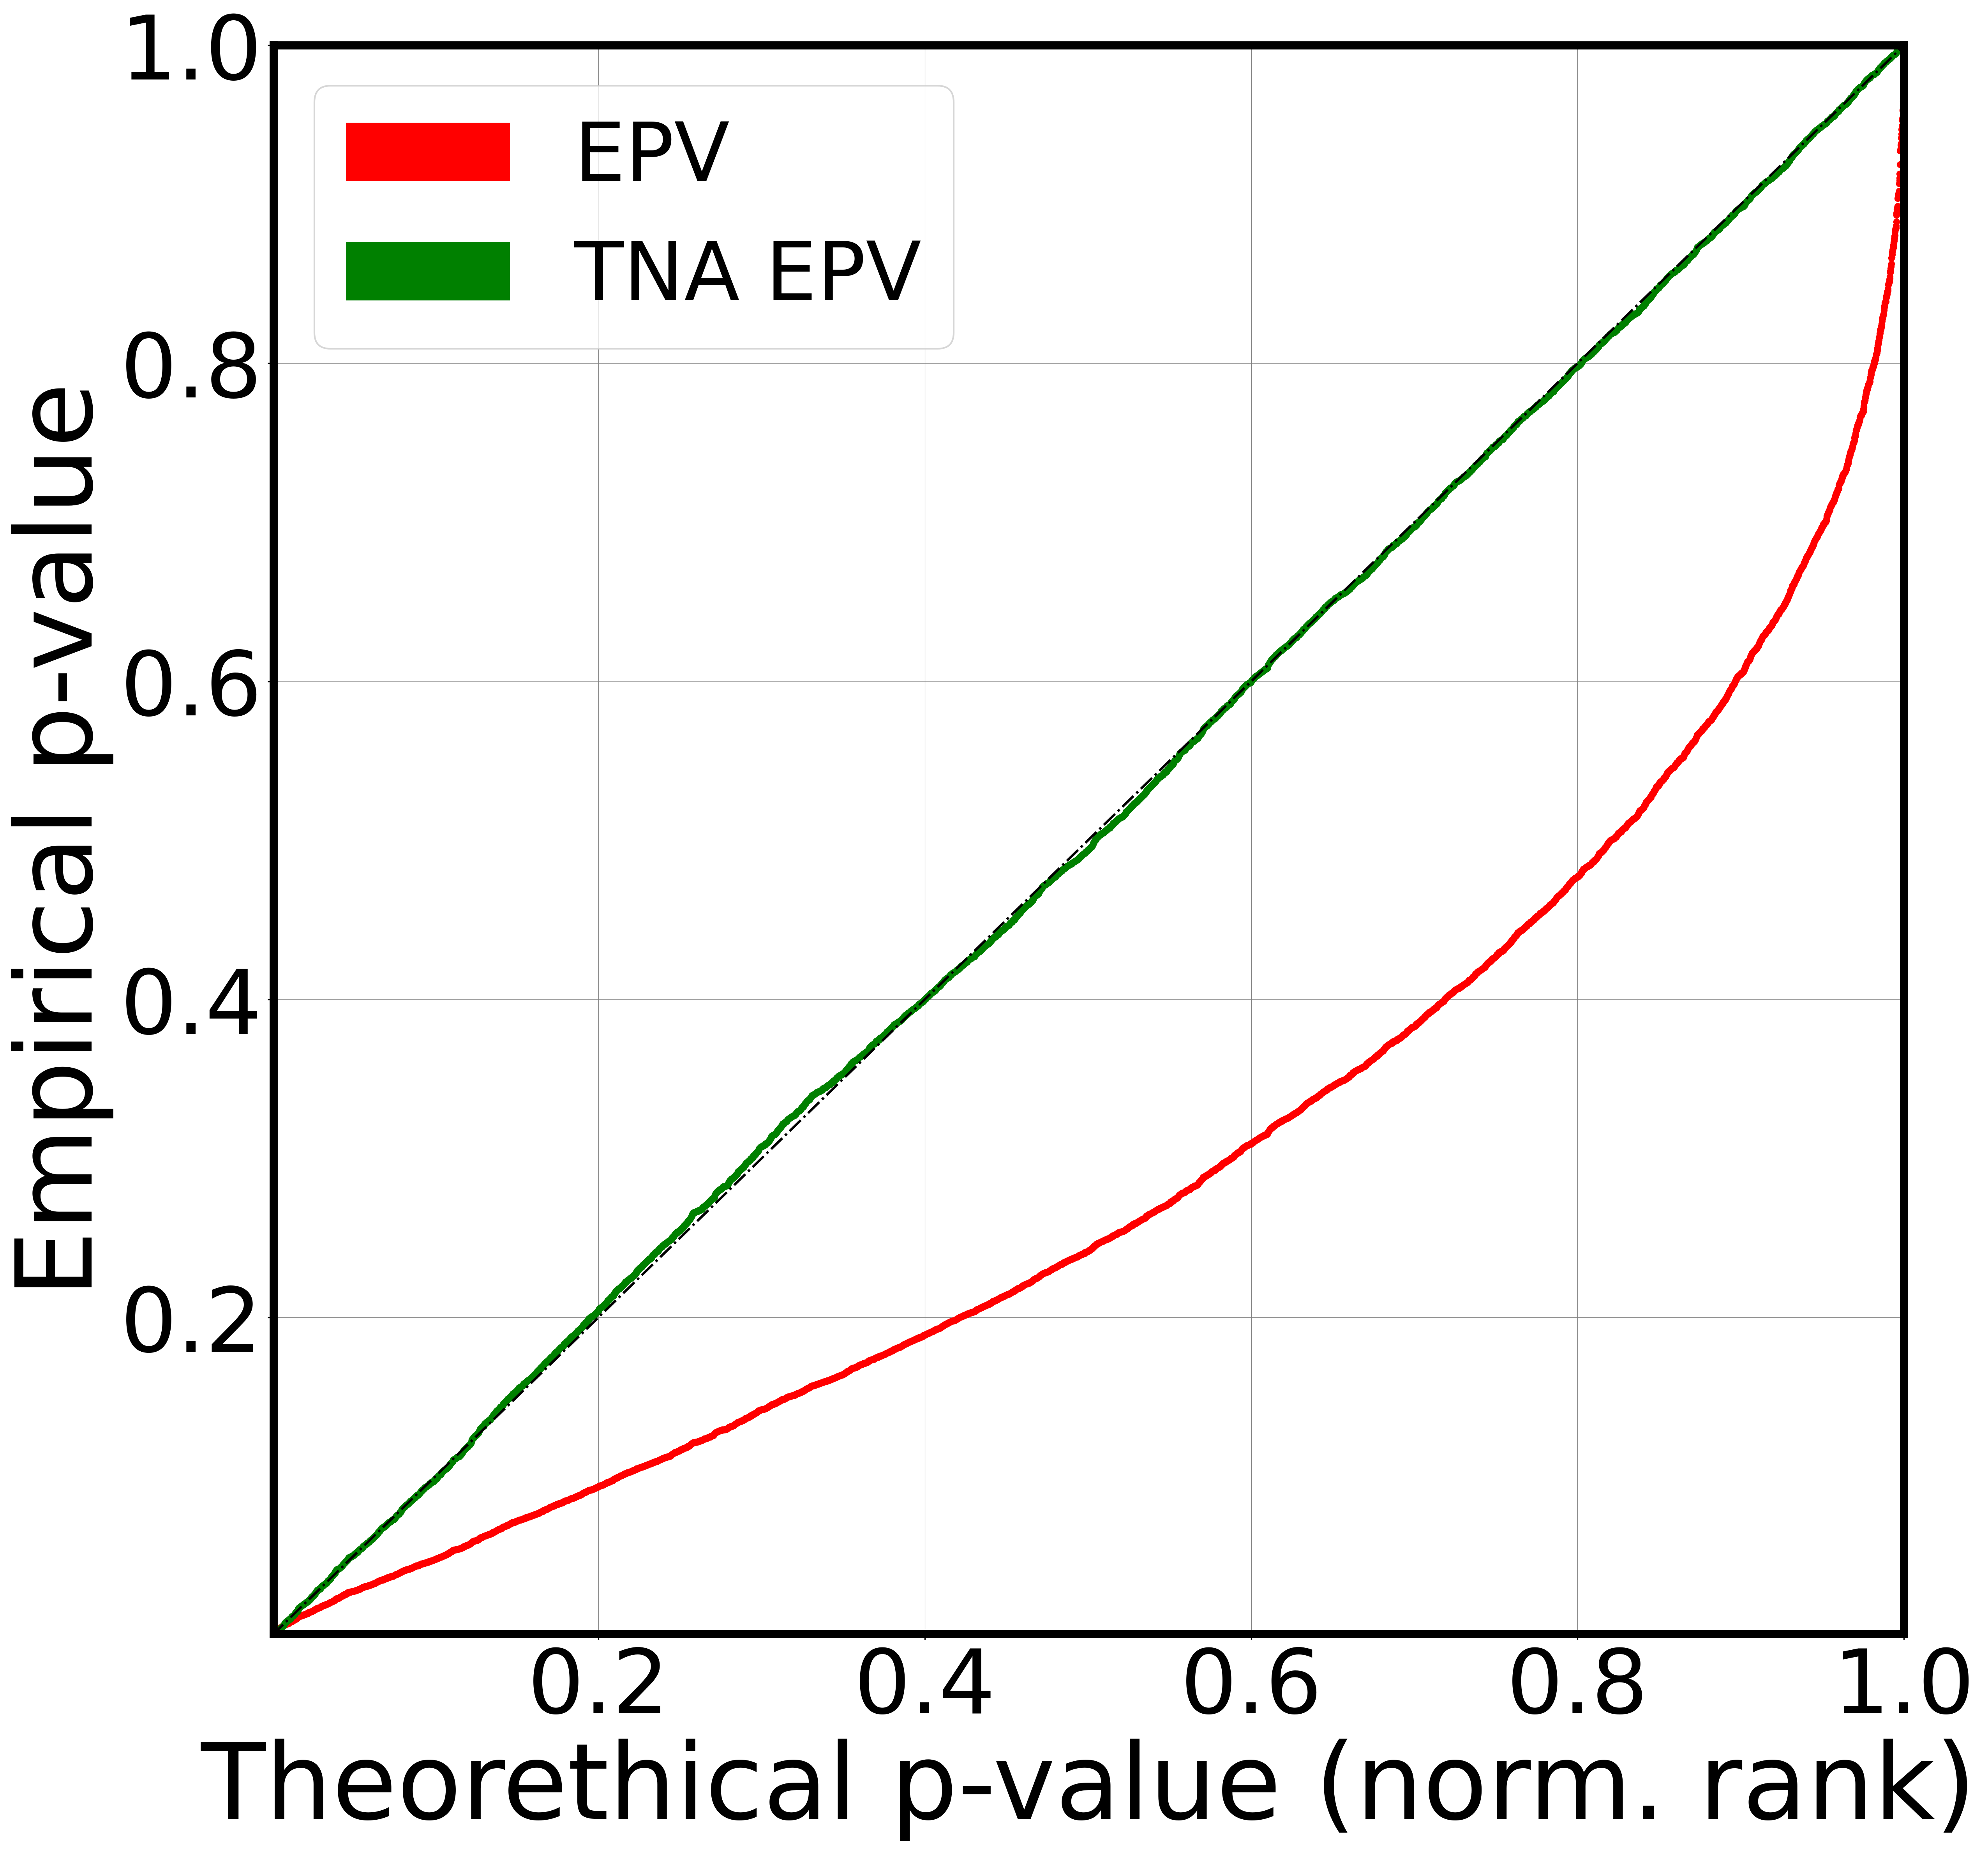
\includegraphics[width=1.7in]{img/cnn_QQ_intensity_down.png}&
		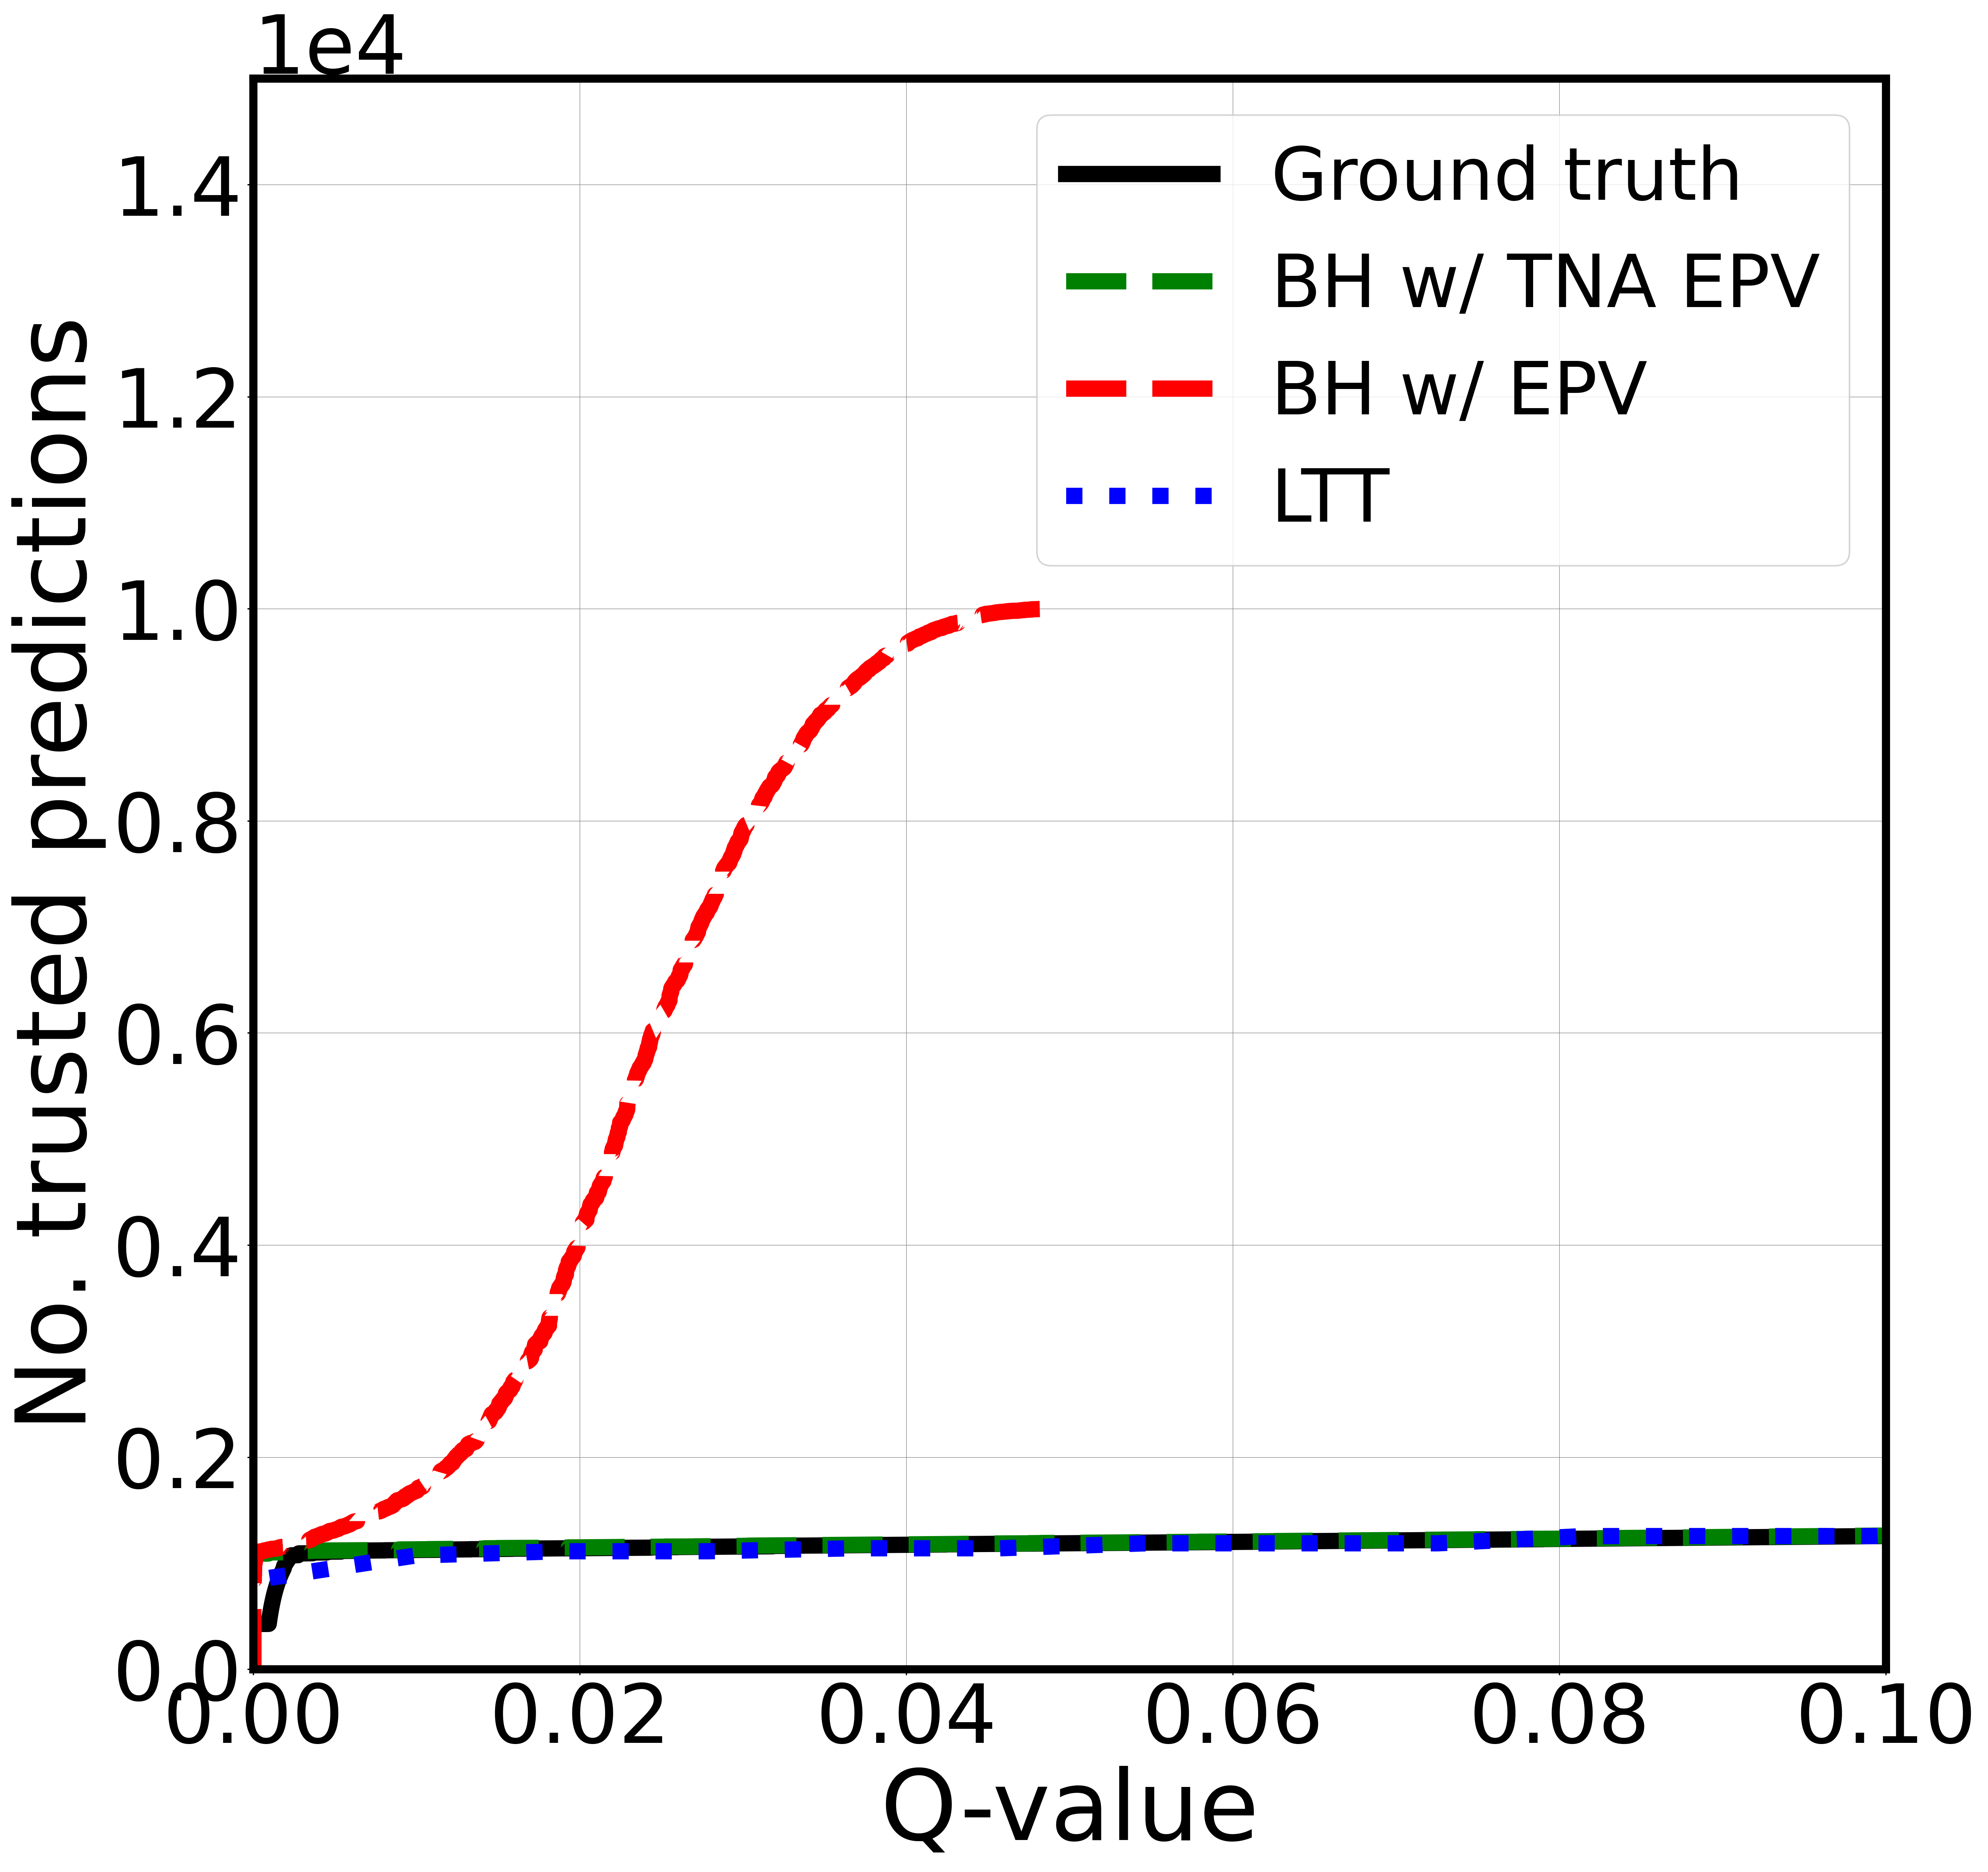
\includegraphics[width=1.7in]{img/cnn_intensity_down_fdr_control_loc.png} &
		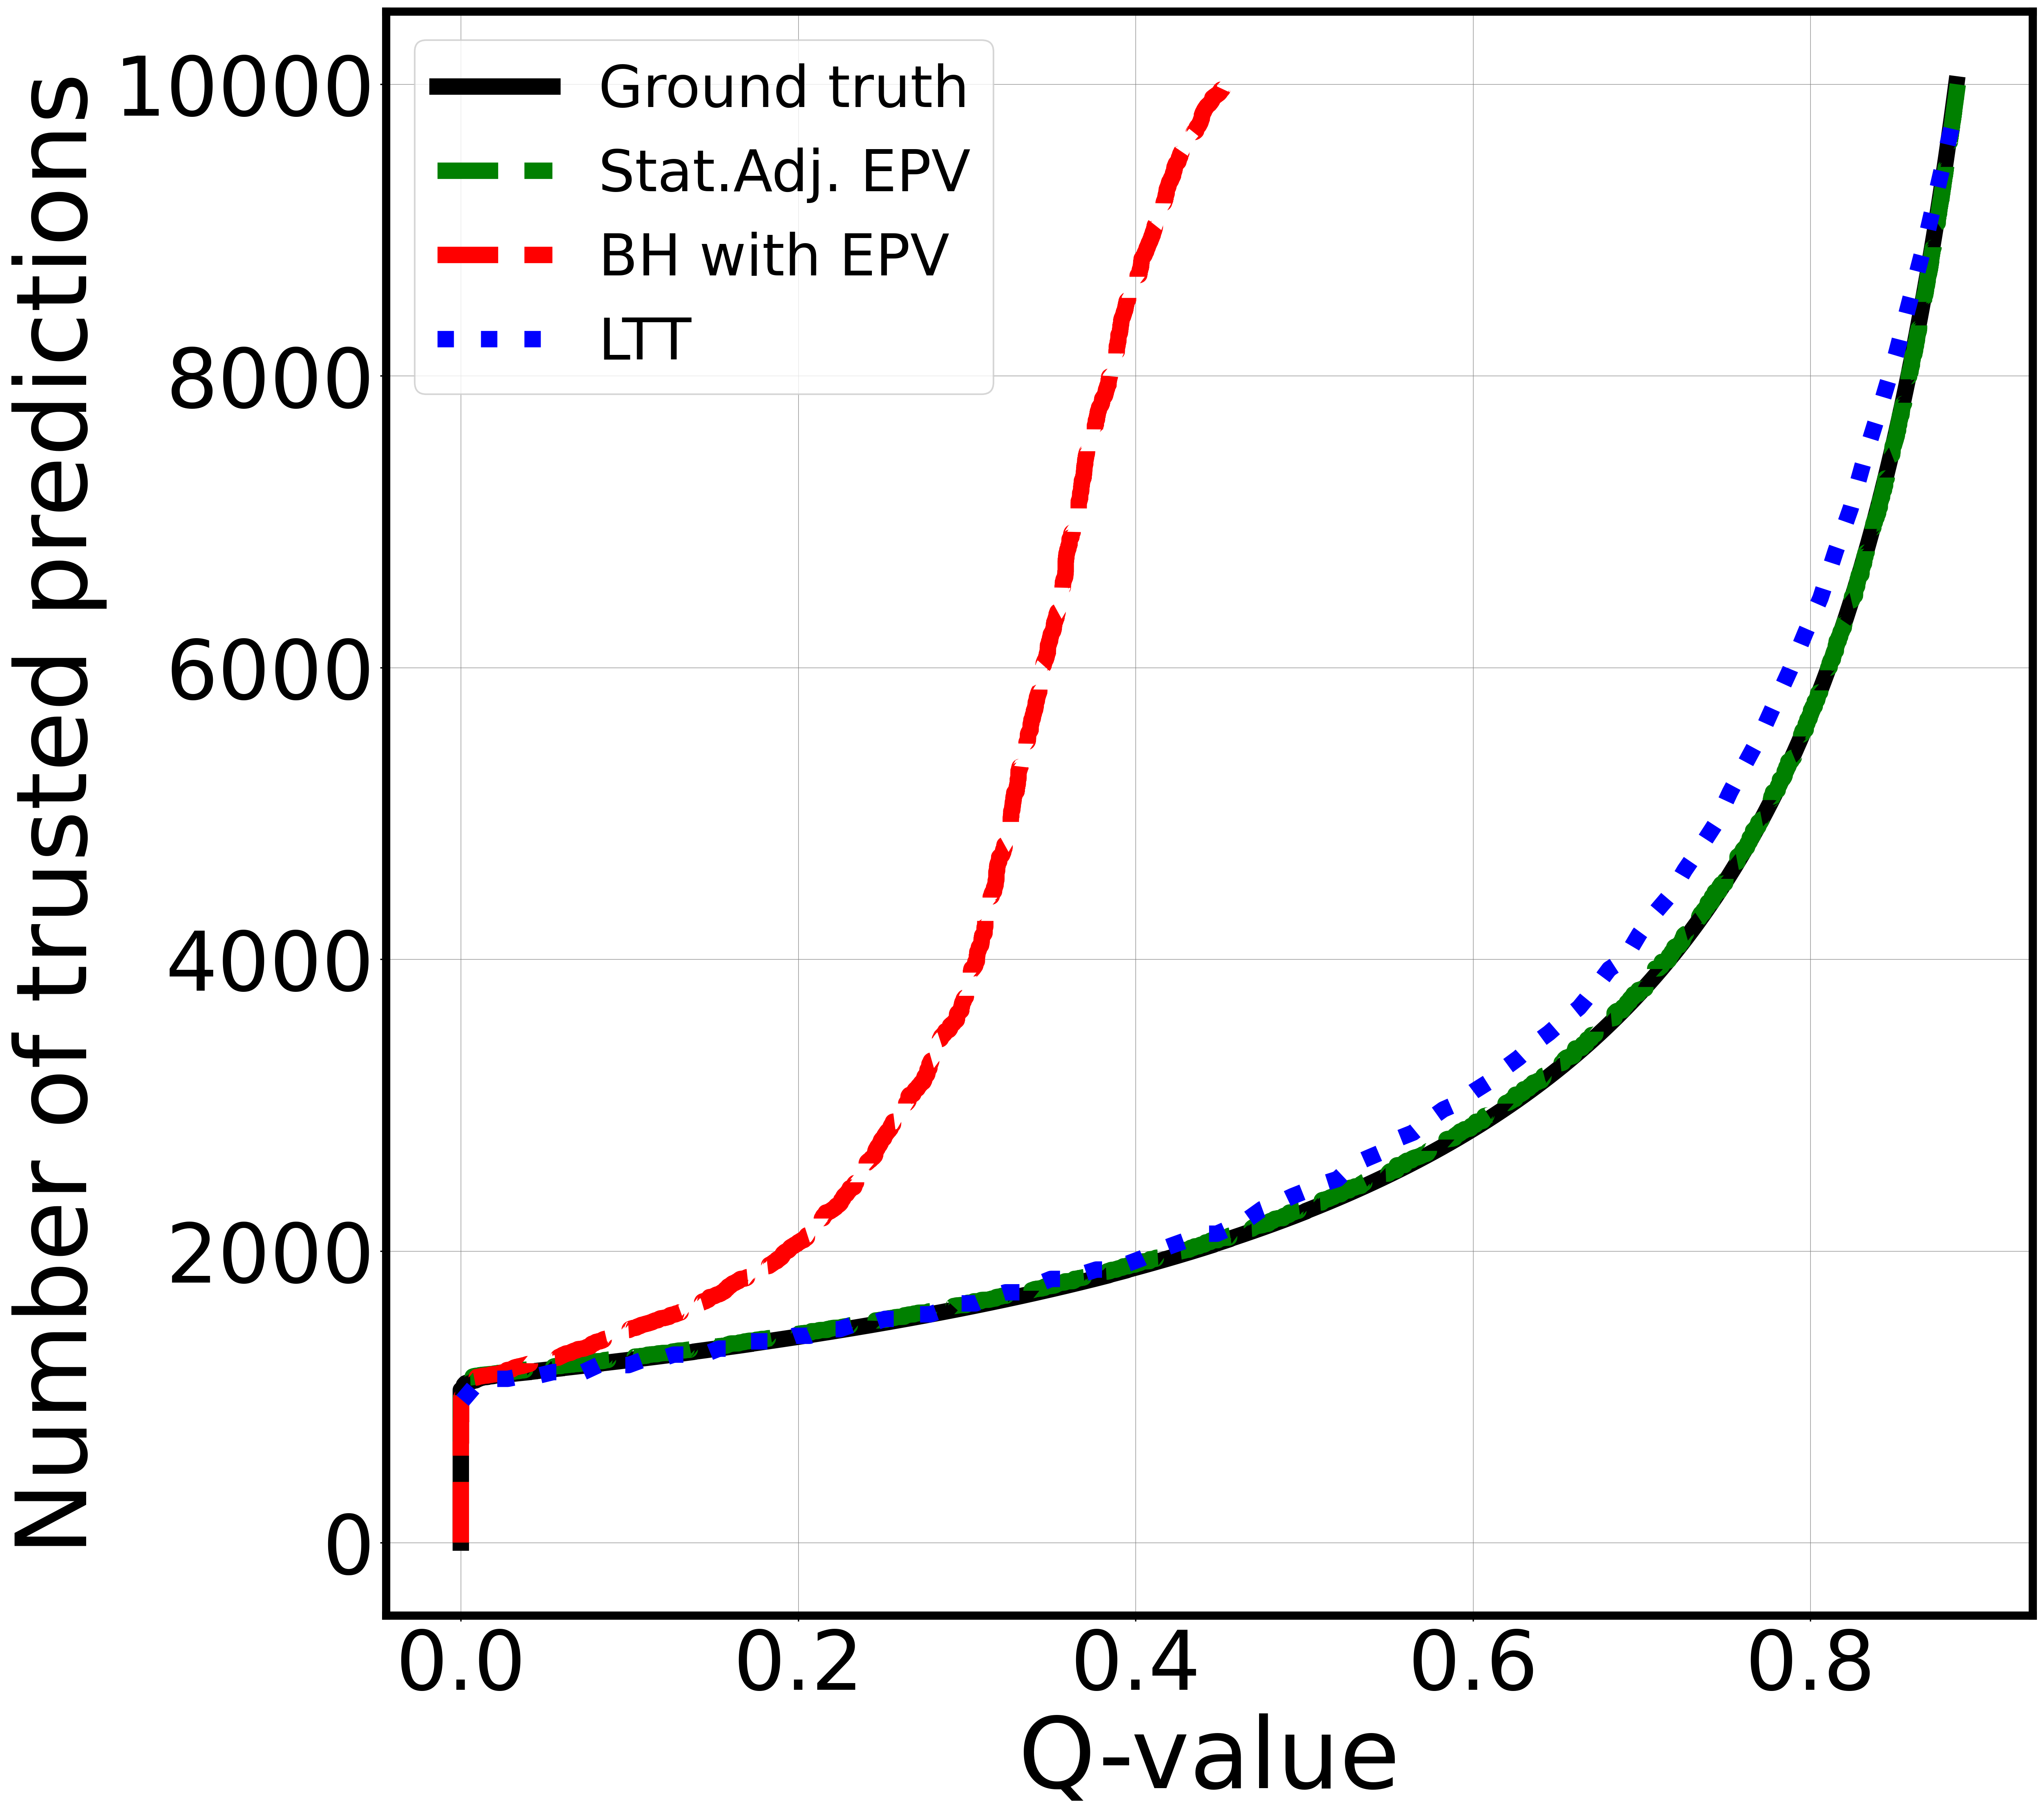
\includegraphics[width=1.7in]{img/cnn_intensity_down_fdr_control.png} & 
		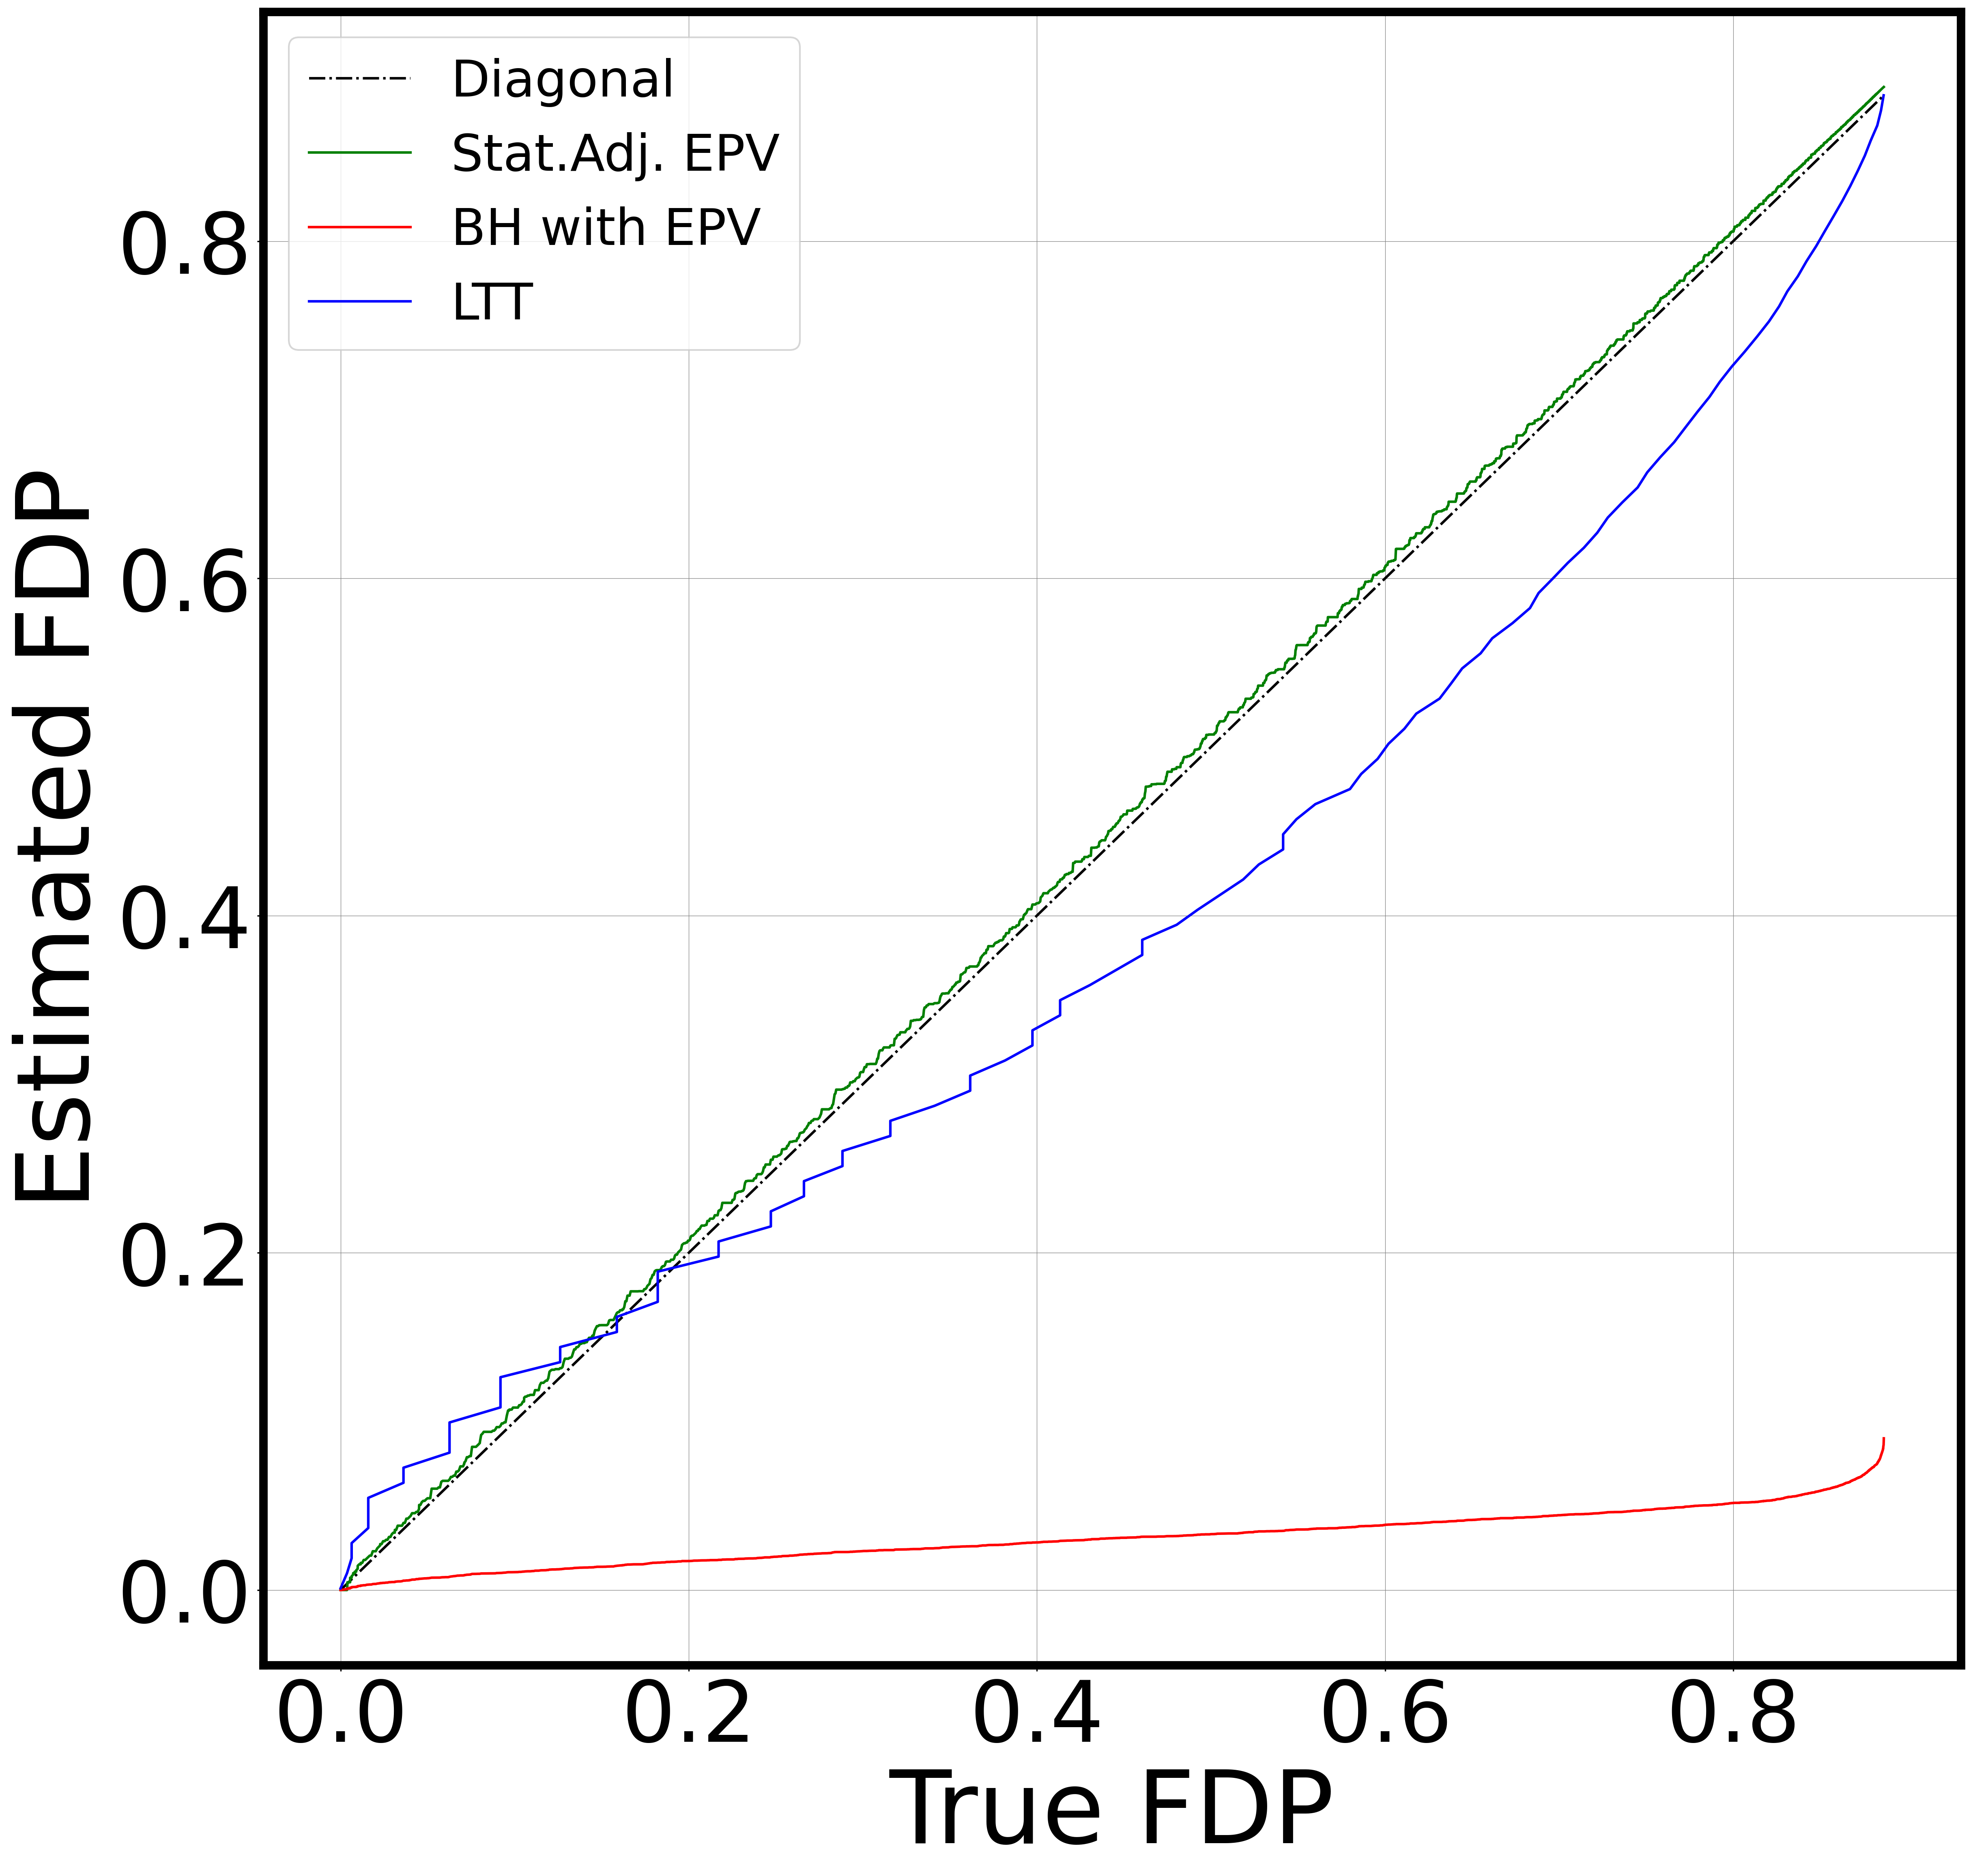
\includegraphics[width=1.7in]{img/cnn_FDPscat_intensity_down.png} \\
		\multicolumn{4}{l}{\bf (ii) Class distribution shit:}\\
		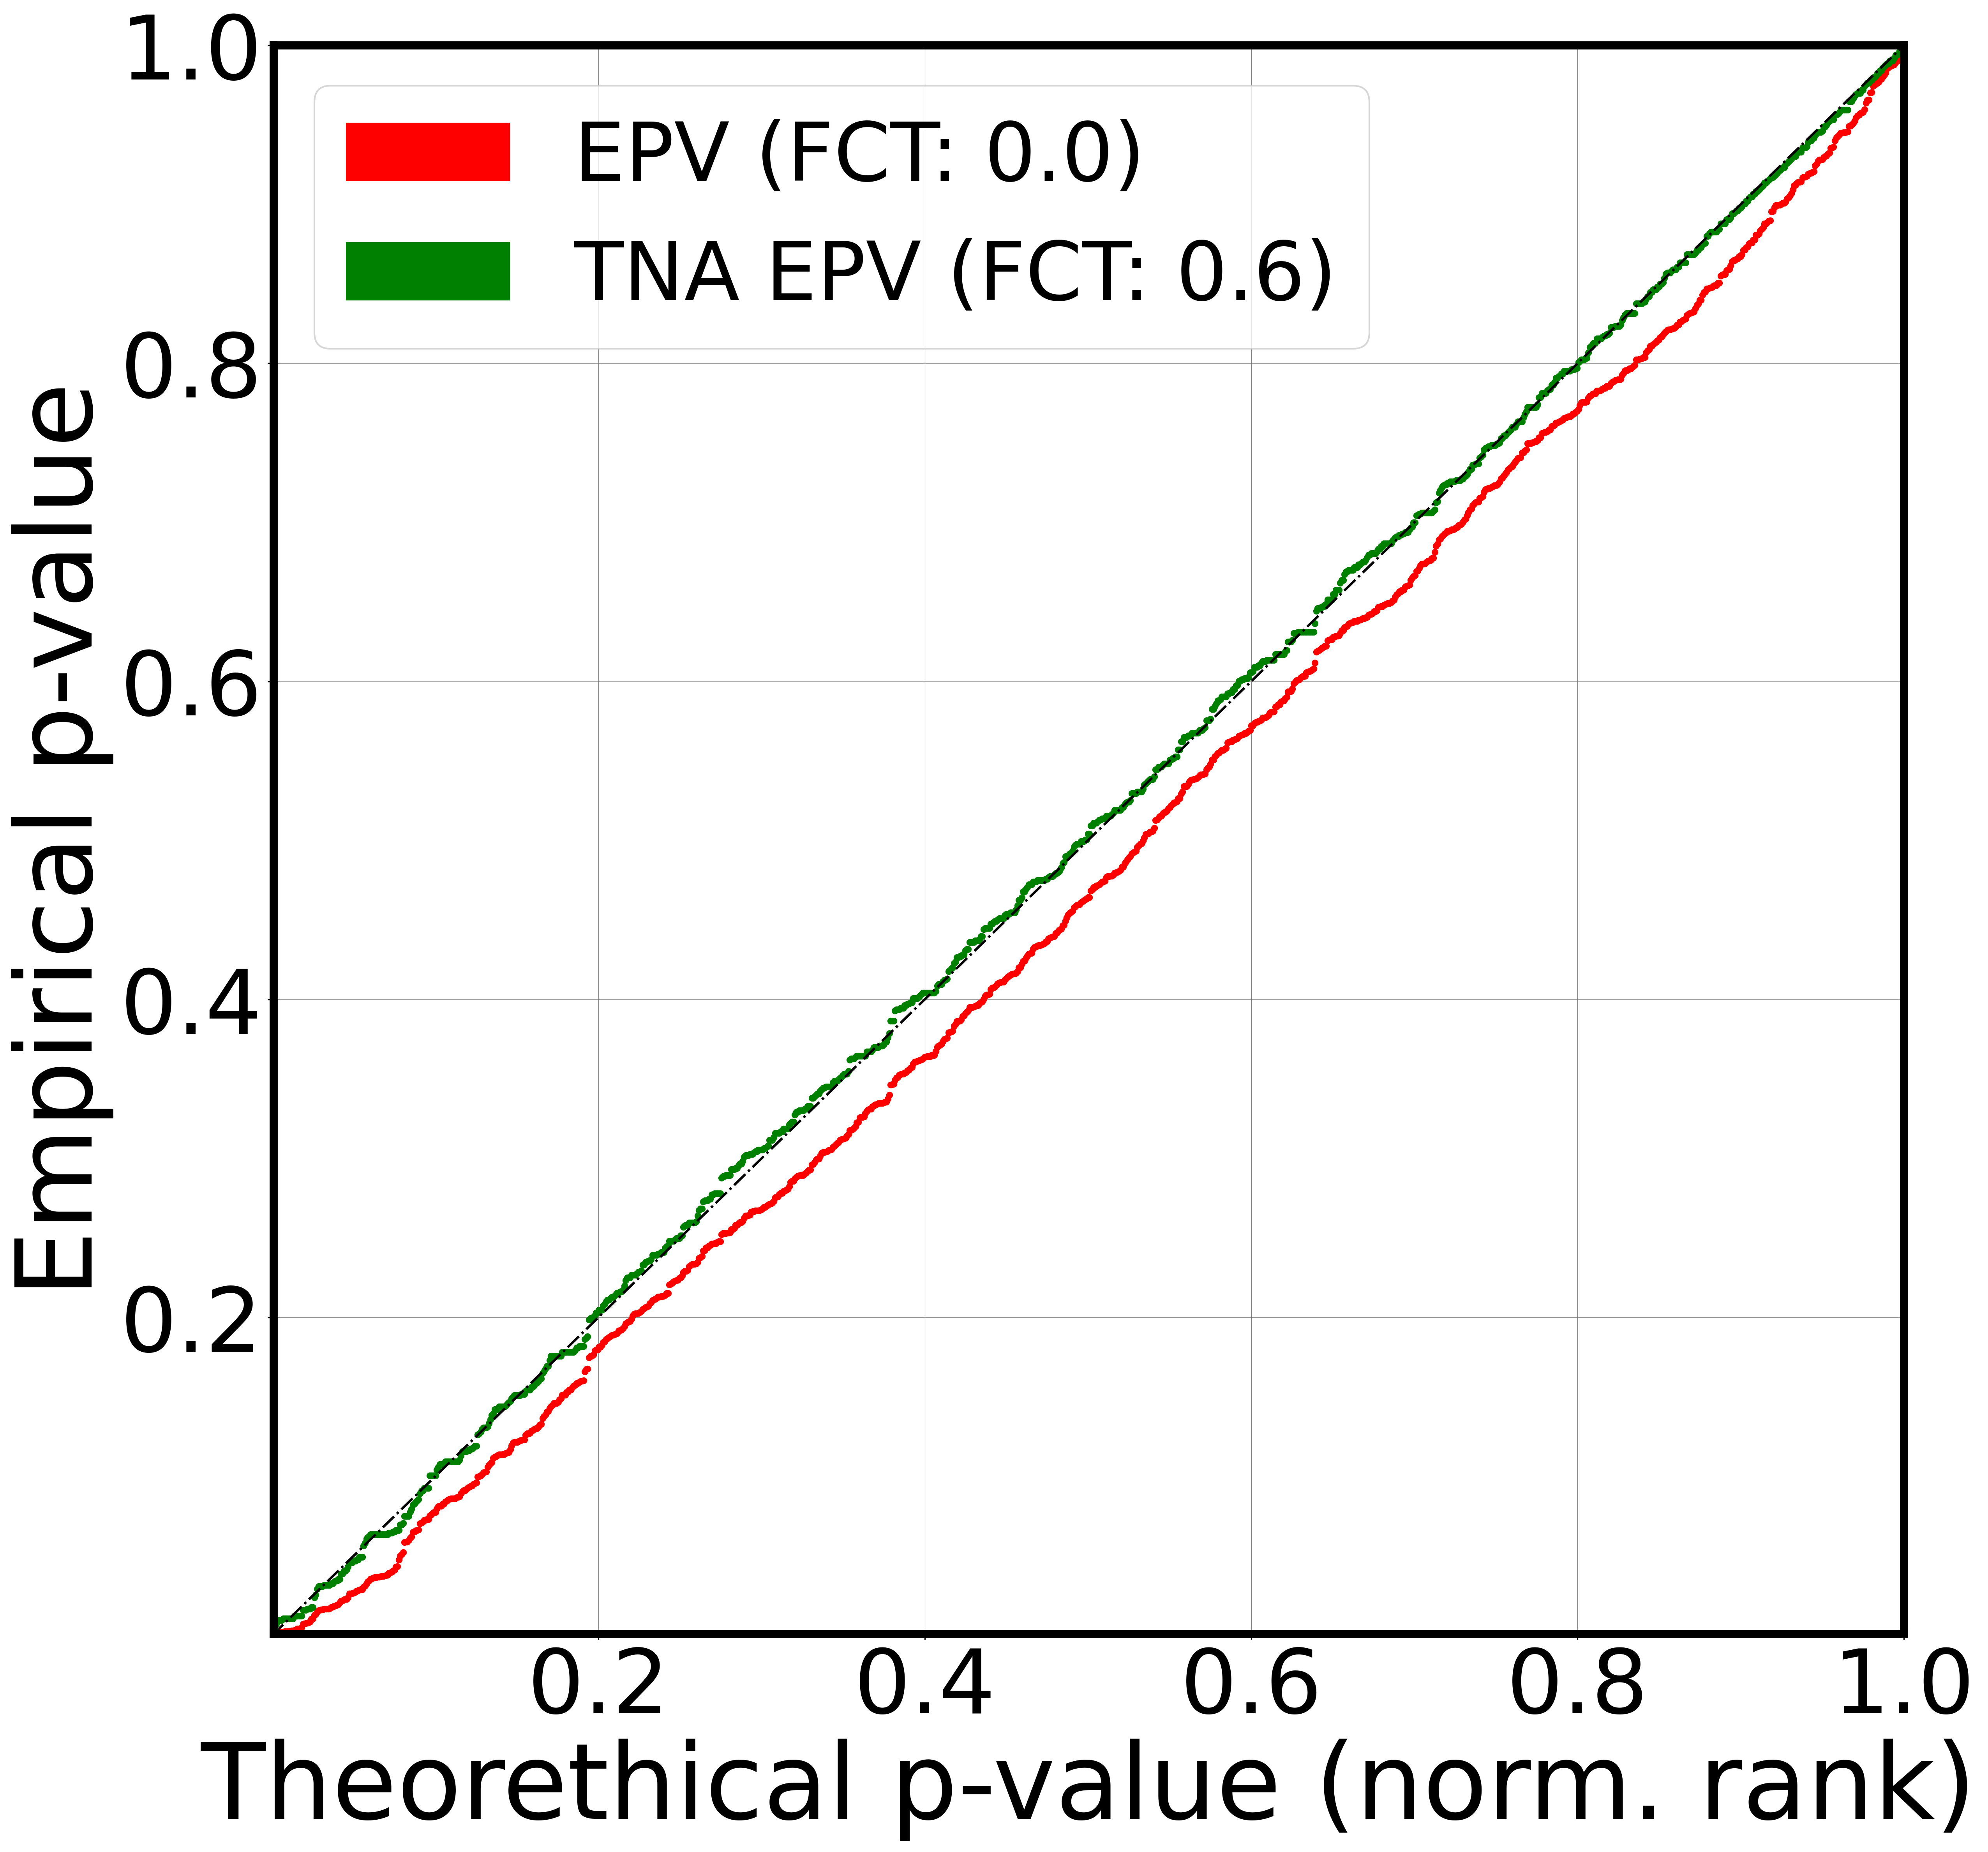
\includegraphics[width=1.7in]{img/cnn_QQ_balanced.png}&
		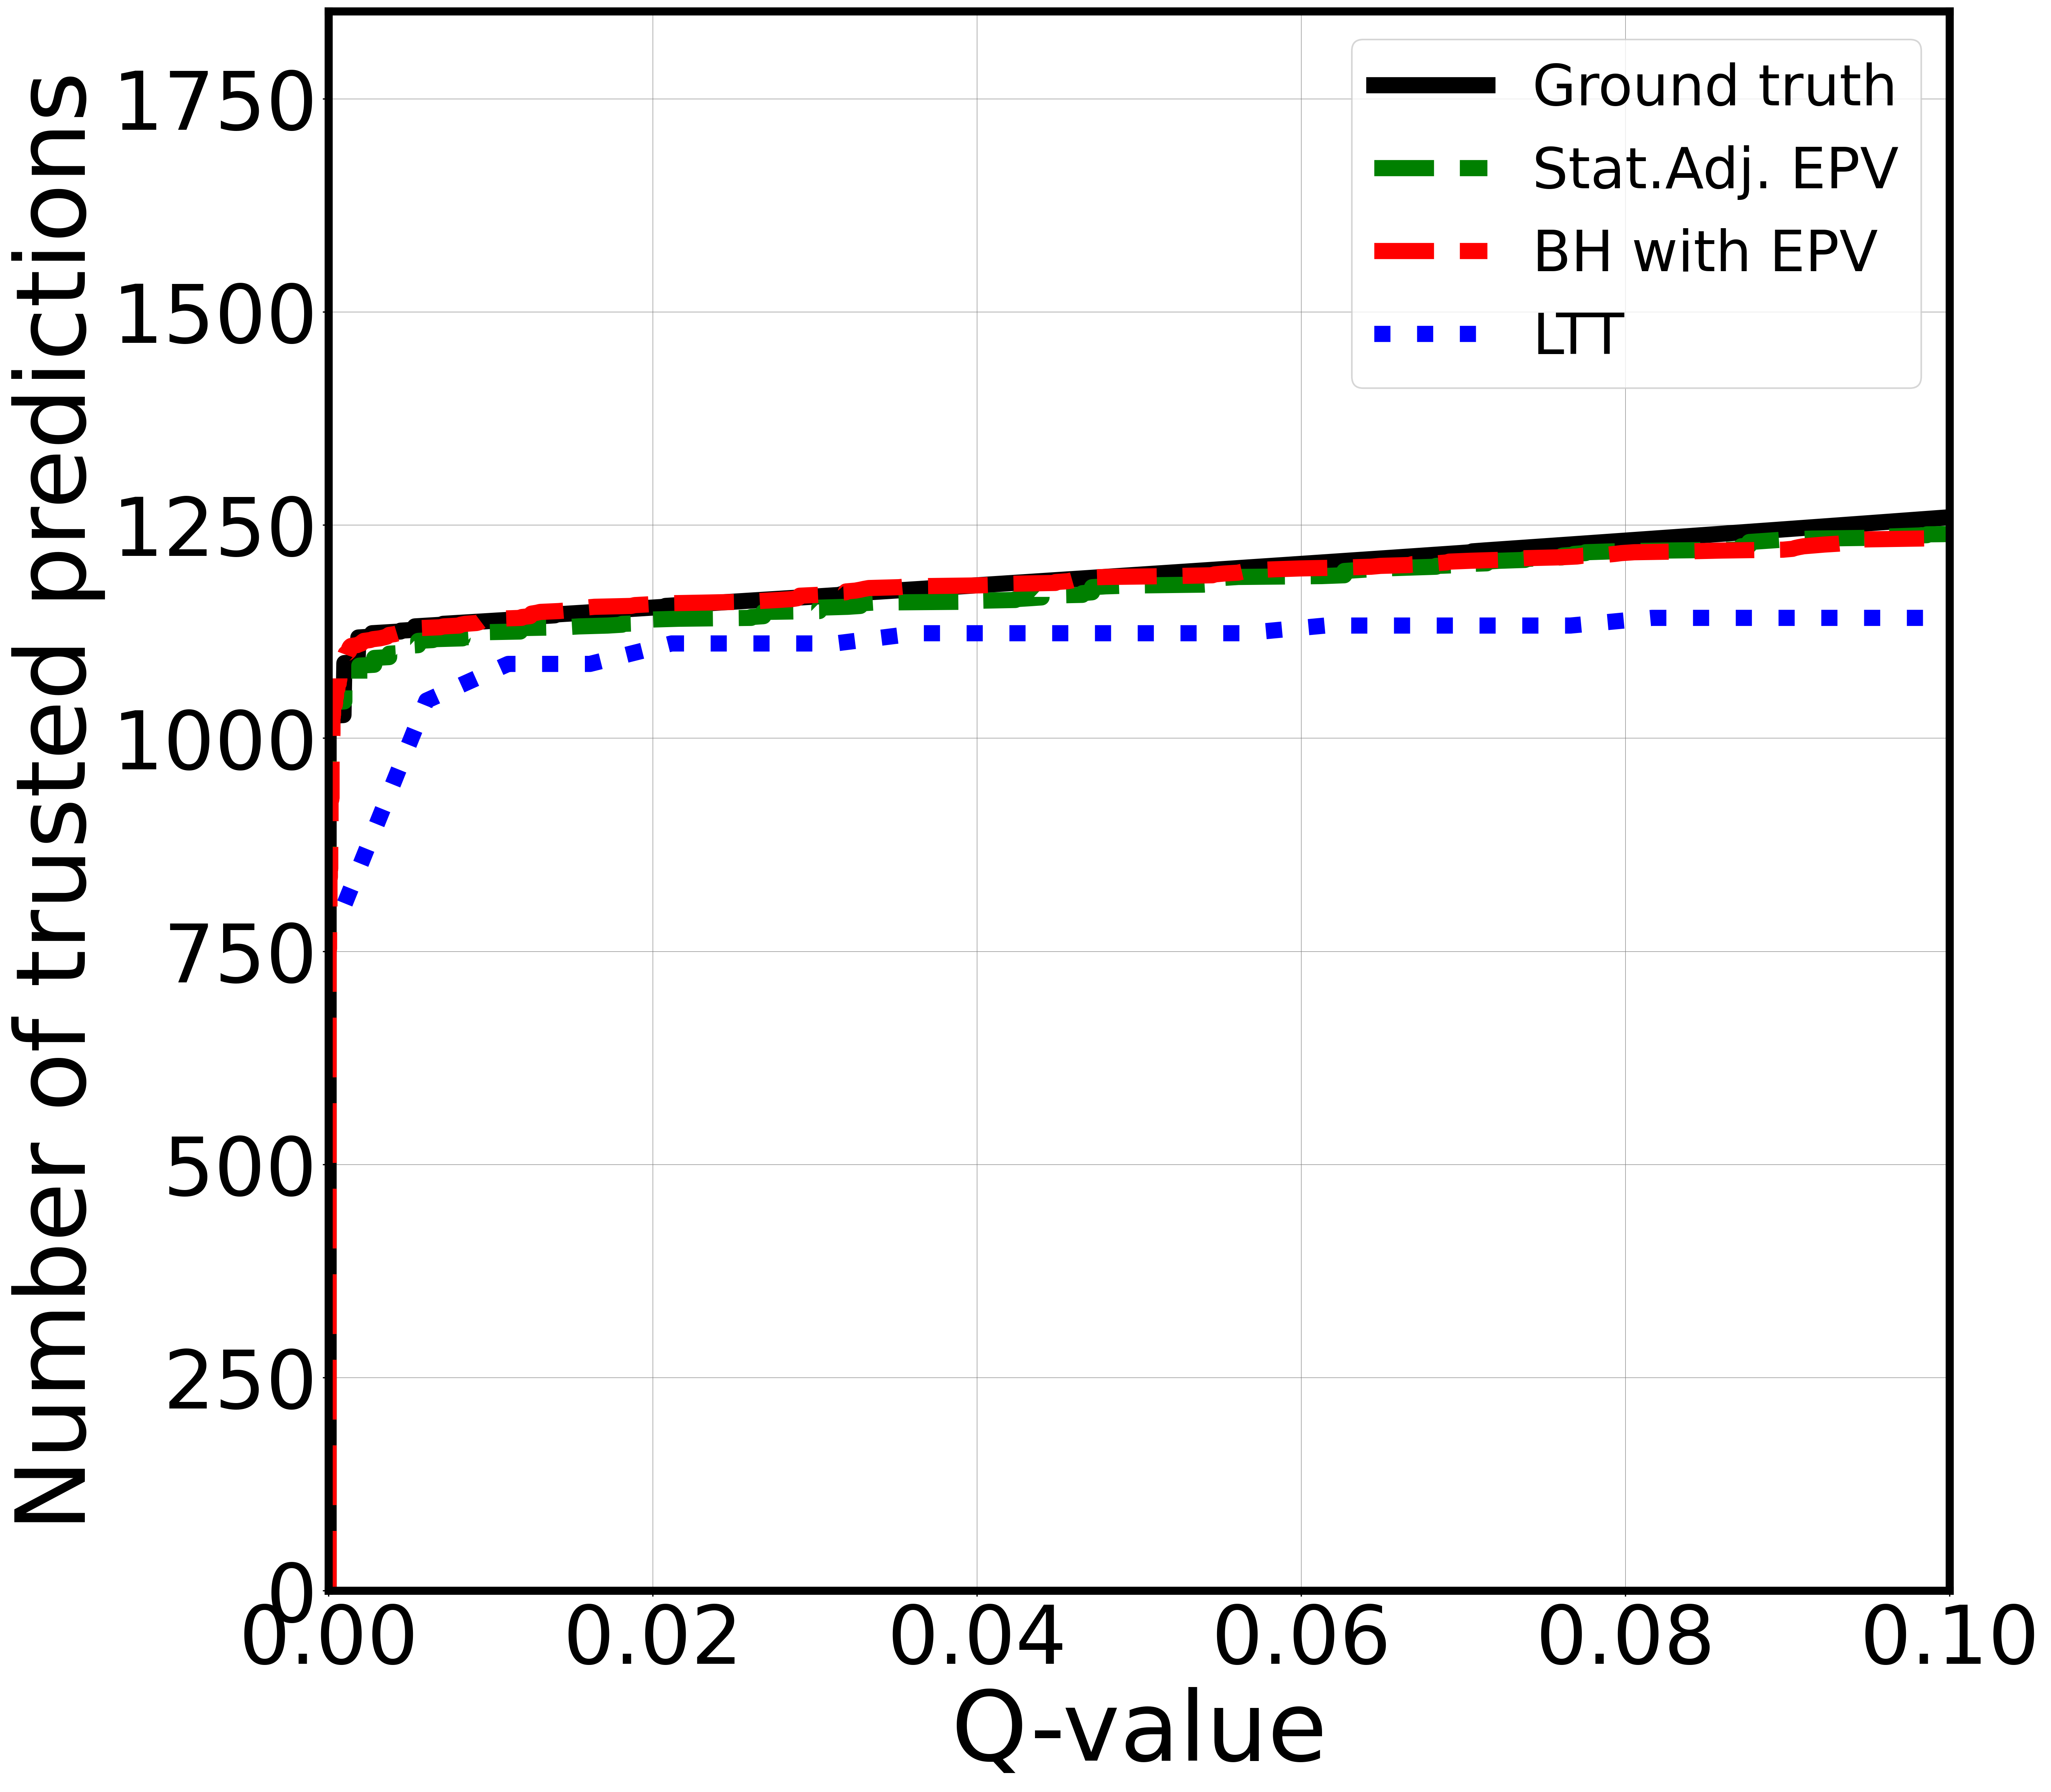
\includegraphics[width=1.7in]{img/cnn_balanced_fdr_control_loc.png} &
		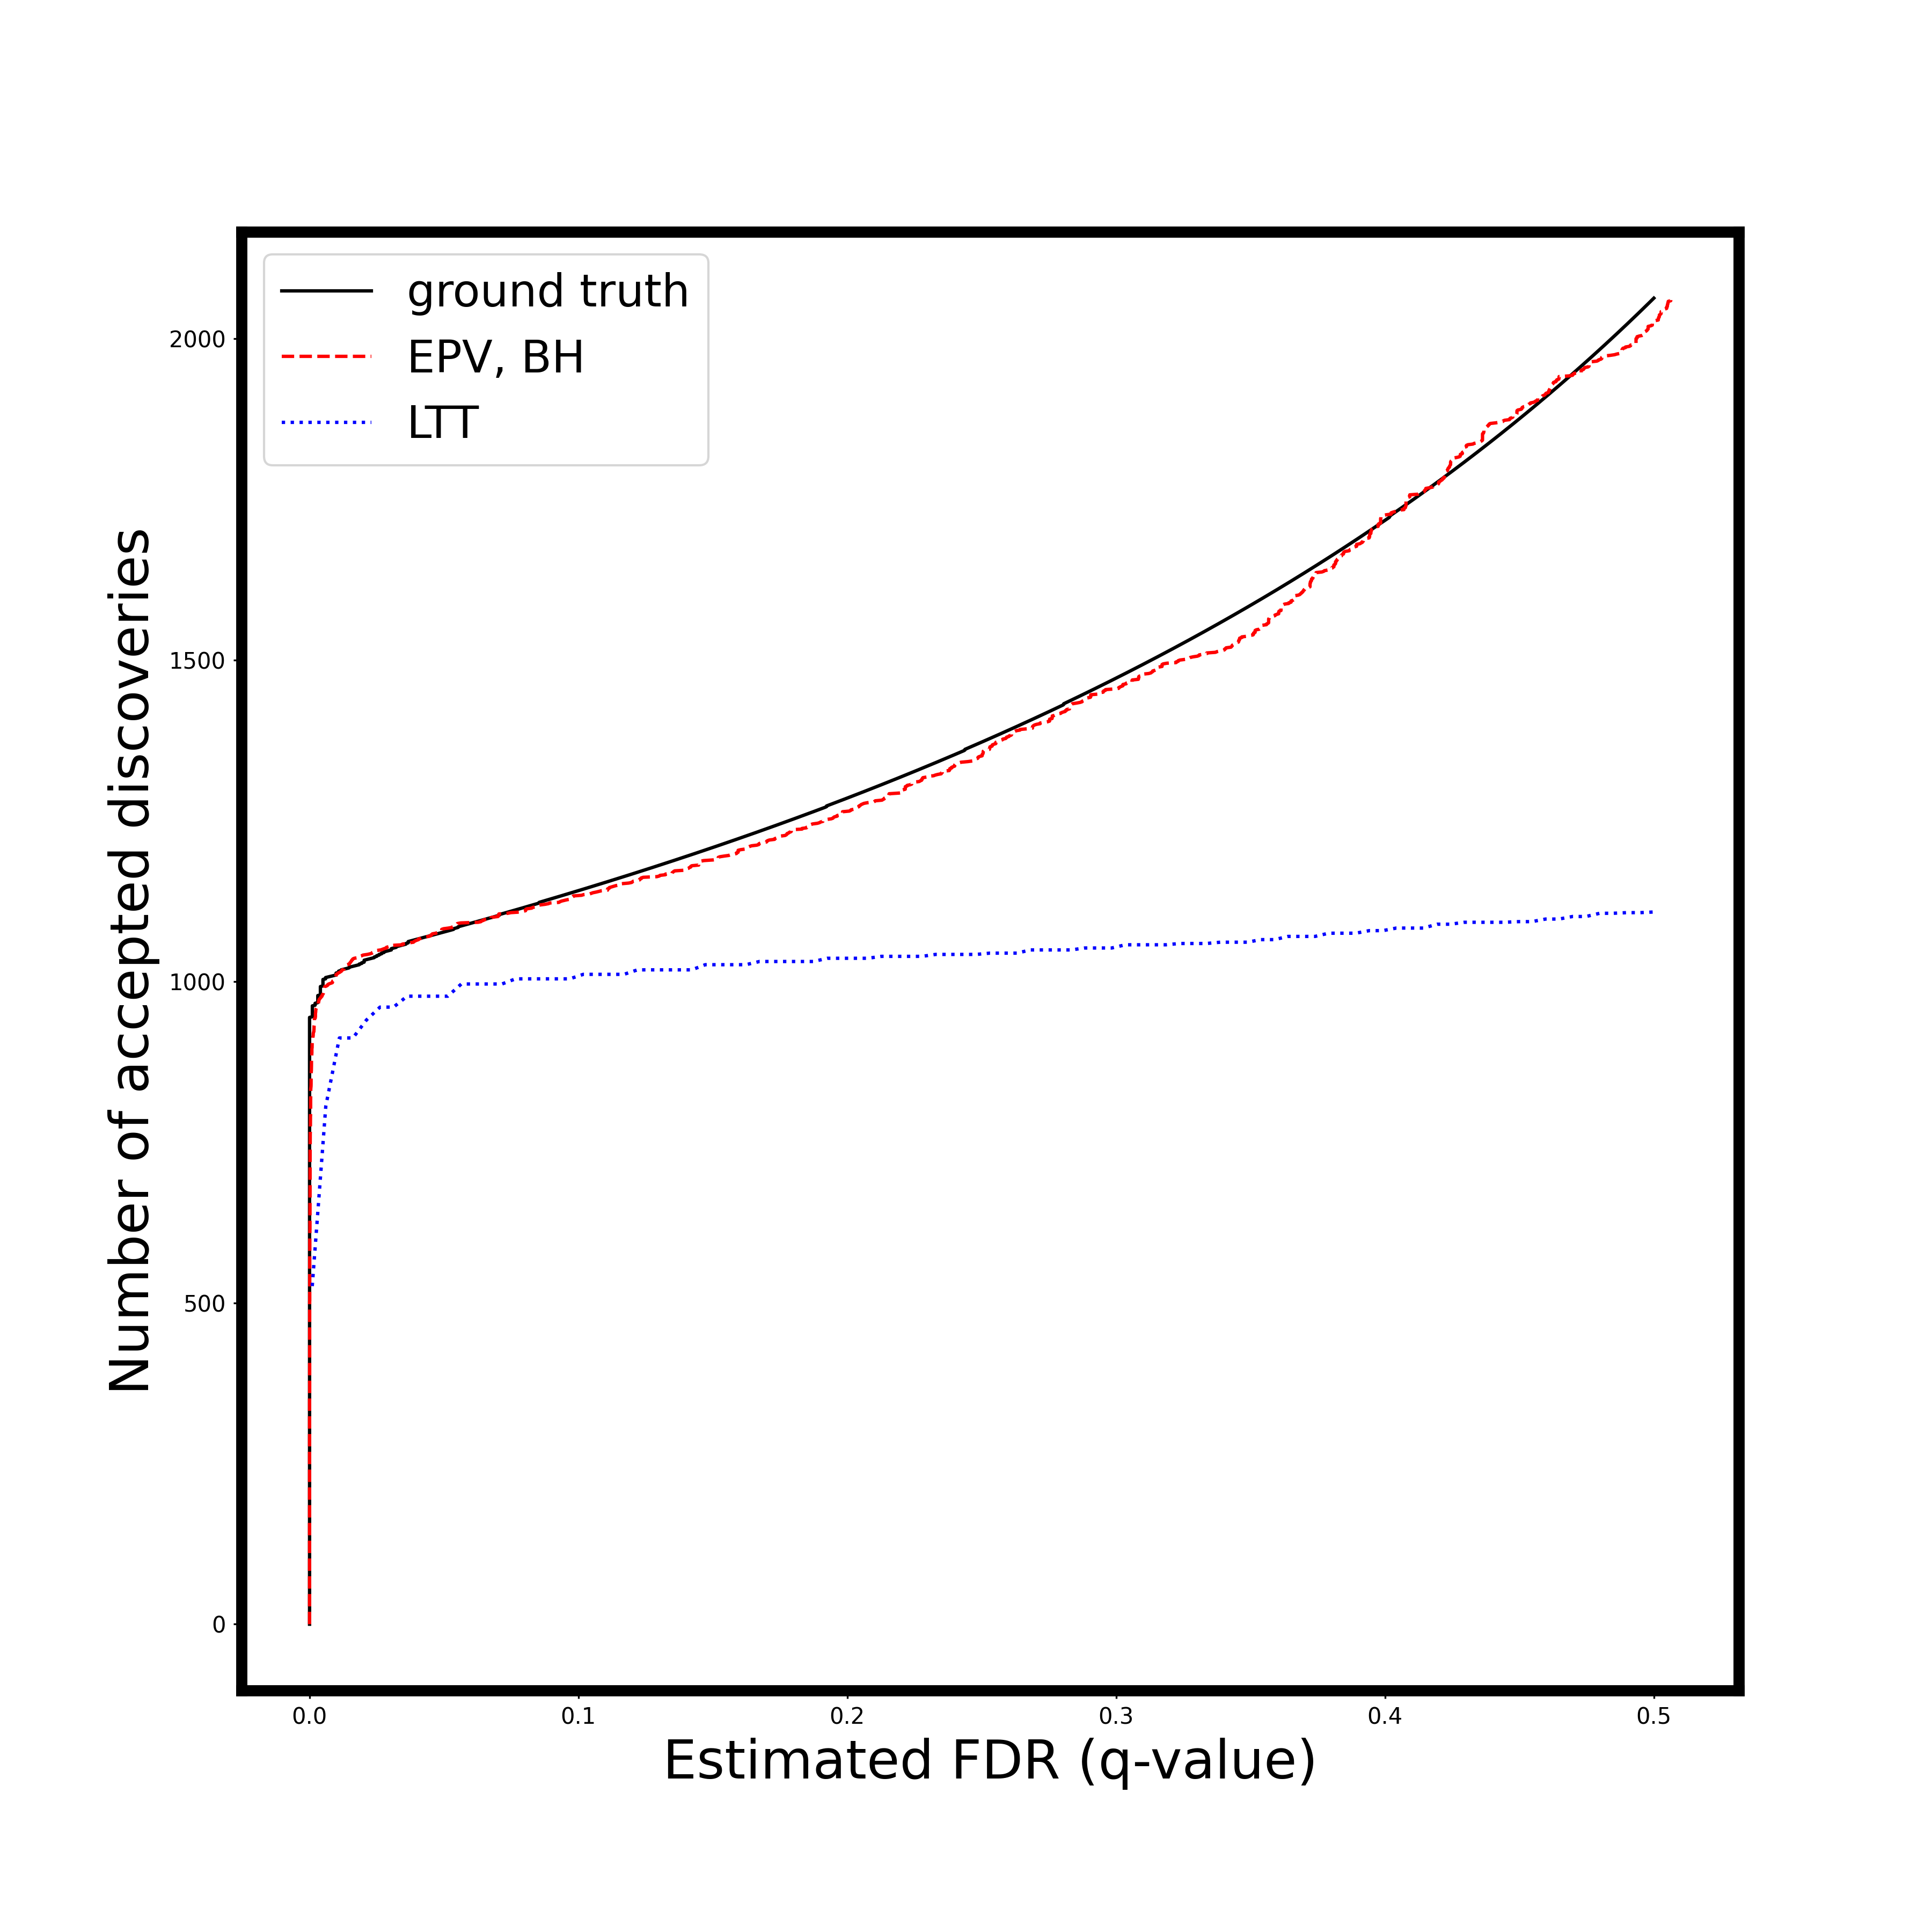
\includegraphics[width=1.7in]{img/cnn_balanced_fdr_control.png} & 
		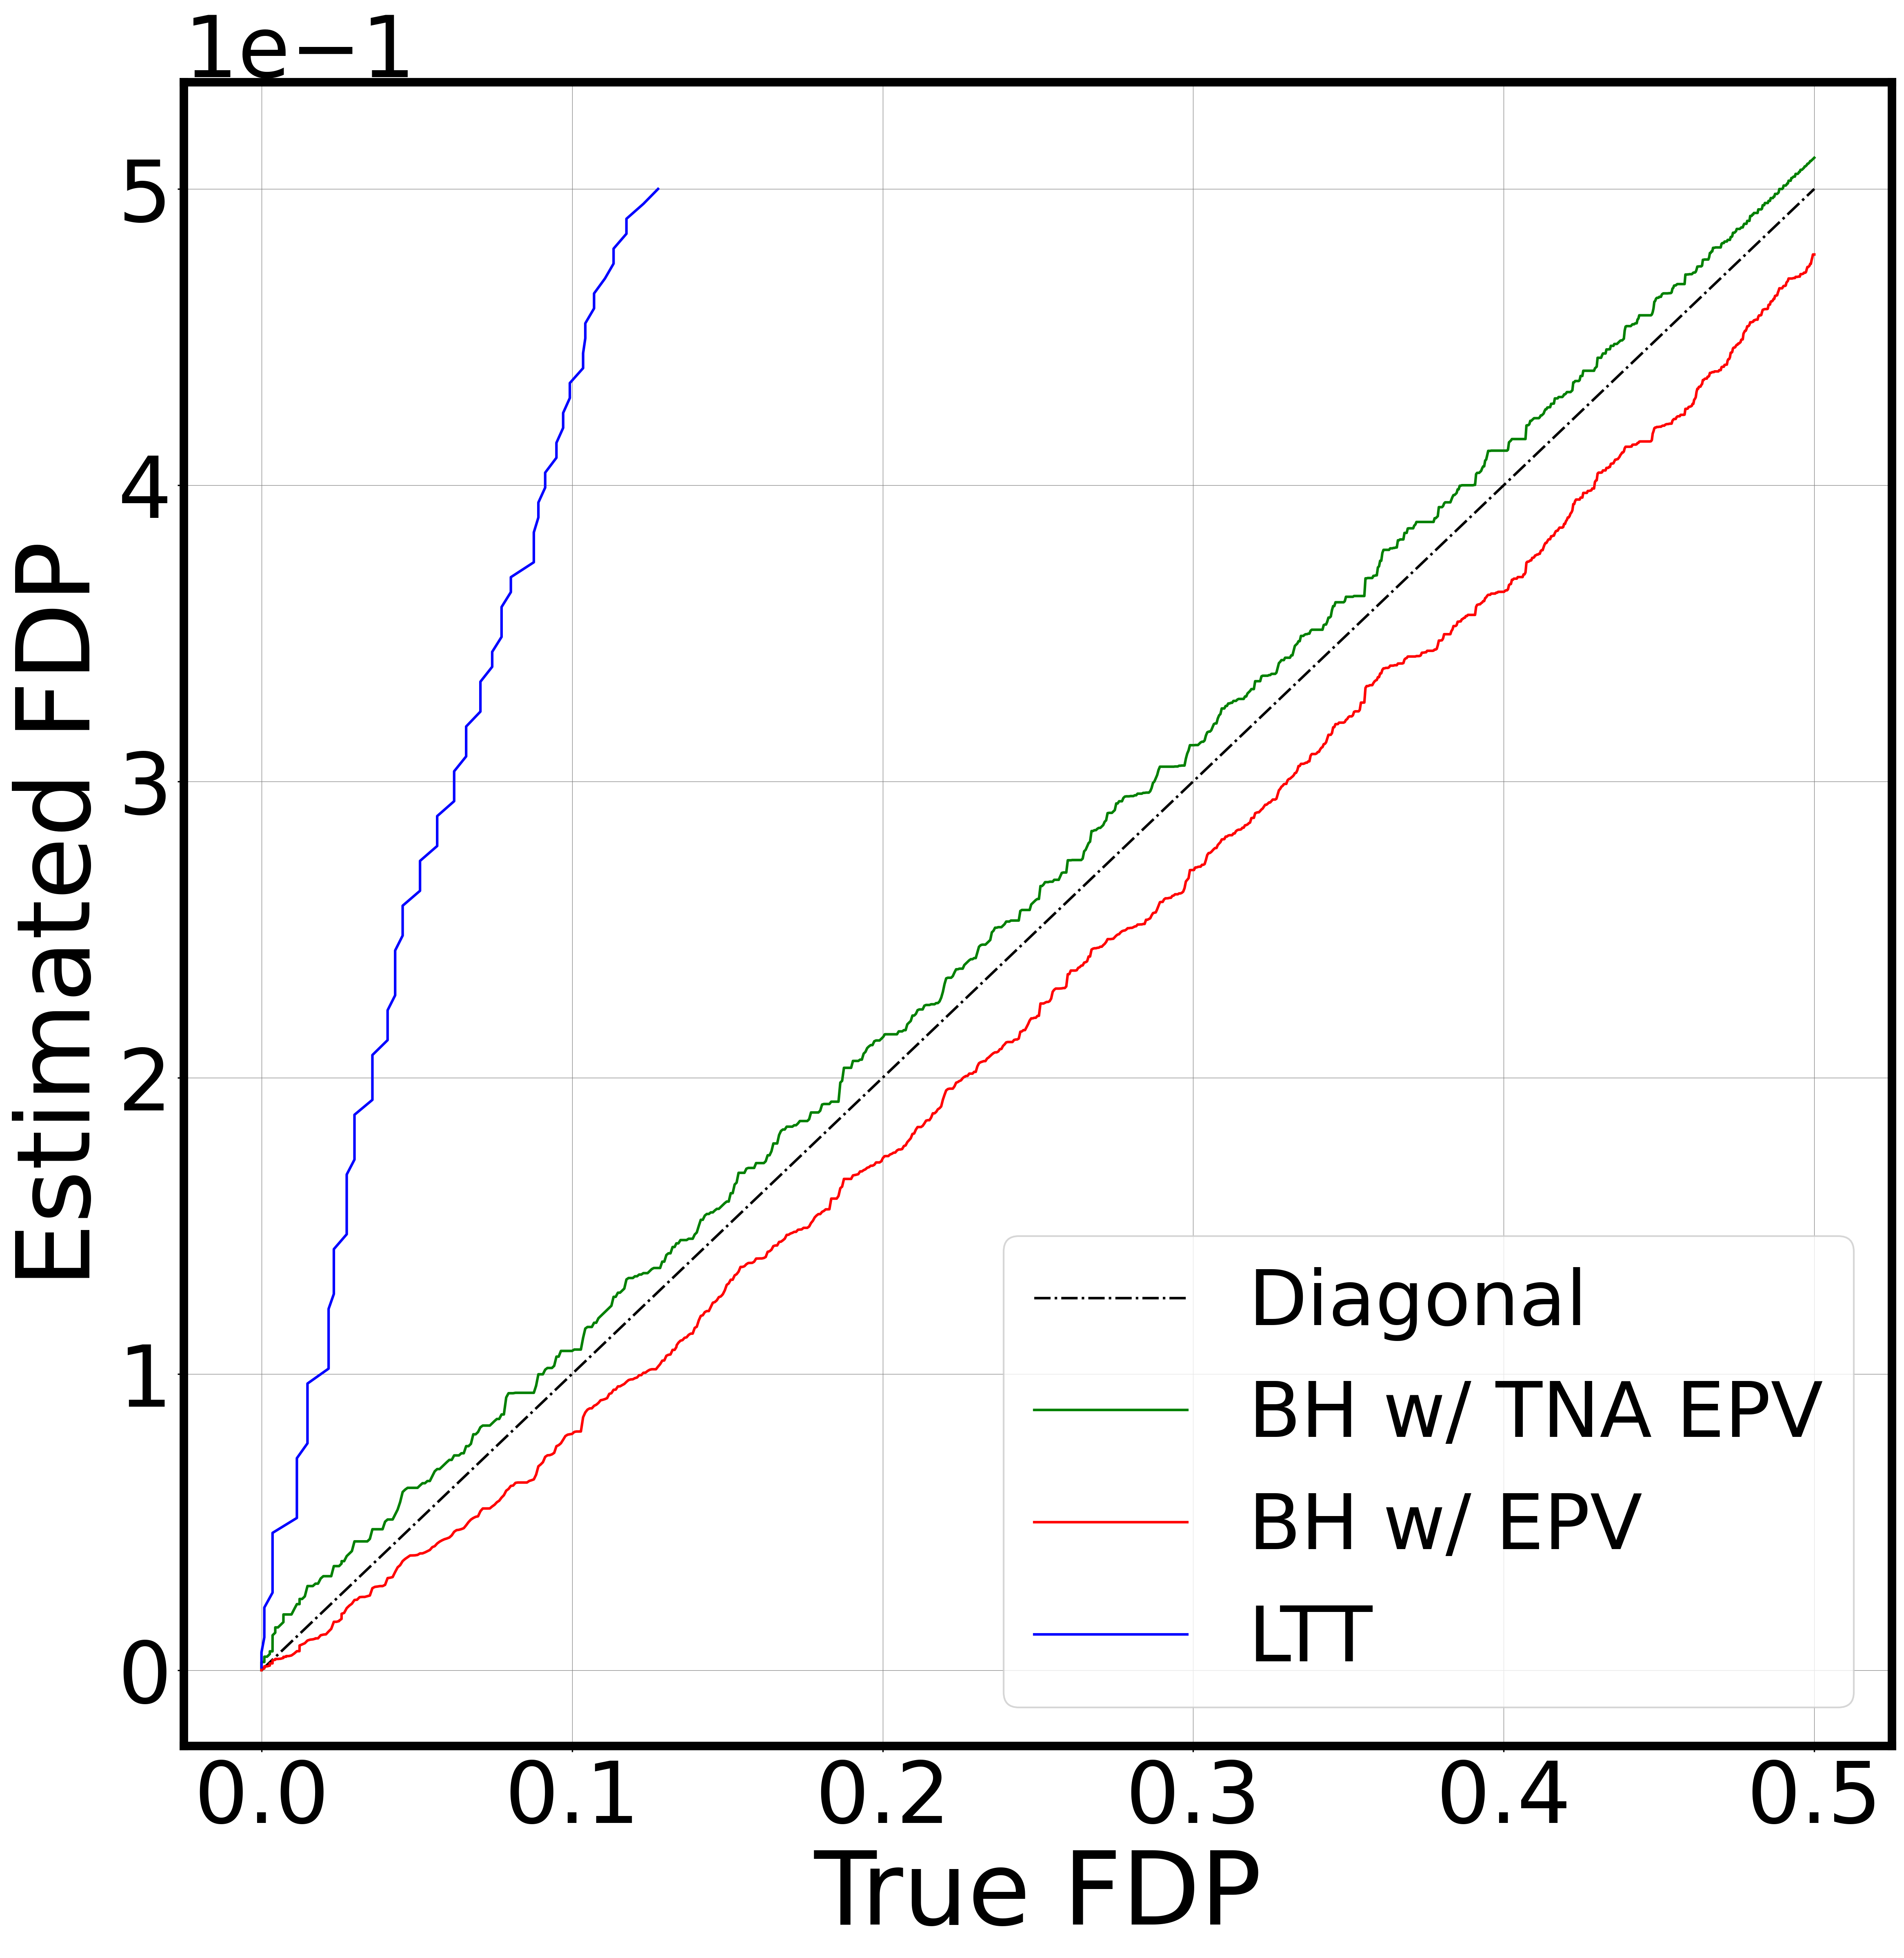
\includegraphics[width=1.7in]{img/cnn_FDPscat_balanced.png} \\		
		A & B & C & D \\
	\end{tabular}
	\caption{{\bf  FDR control with empirical p-values.}
		(A) QQ plot of the EPVs (red dots) and the EPVs with TNA (green dots) against the theoretical uniform distribution. The results of the Fisher's combination tests are indicated in the legend. (B) The number of accepted classifications as a function of the Q-values obtained with (i) ground truth (black line), (ii) BH with EPV (red), (iii) BH with EPV with TNA (green), and (iv) LTT (blue). (C) Same as (B) with over the entire Q-value range. (D) Deviation of the estimated FDR from the actual FDR obtained with (i) BH with EPV (red line), (ii) BH with EPV and TNA (green line, (iii) LTT (blue line).}
	\label{fig:mnist_shfit}
\end{figure}

	
\paragraph{Example 2.} To illustrate the case of data distribution shift, we down-scaled the pixel intensity by 10\% of the test images in the MNIST dataset (but train images remained the same). The accuracy of the CNN classifier (the same as trained in Example \ref{ex:vanilla}) remained at 99 \%. The evaluation plots are shown in Figure \ref{fig:mnist_shfit}-(i). The plots and tests show that standard EPVs became biased in the case of data distribution shift; however, TNA can correct the EPVs so that FDR control becomes unbiased.


\paragraph{Example 3.} To illustrate the case of class distribution shift, we resampled the test data so that number of true negative and positive instances are equal. This approach was used in other articles, e.g.  \cite{joseph_d__viviano__2019}. The accuracy of the CNN classifier (the same as trained in Example \ref{ex:vanilla}) remaind at 99 \%. The evaluation plots are shown in Figure \ref{fig:mnist_rebalance}-(ii). The results show that, in general, the EPV methods can adjust to the changed class proportions thanks to the $\pi_0$ estimation among the test instances for the BH protocol. However, the LTT method calibrates its parameters about class proportion with using a validation set, hence it becomes biased when class proportion change in the test data. 
%
%\begin{figure}[h!]
%	\centering
%	\begin{tabular}{cccc}
%		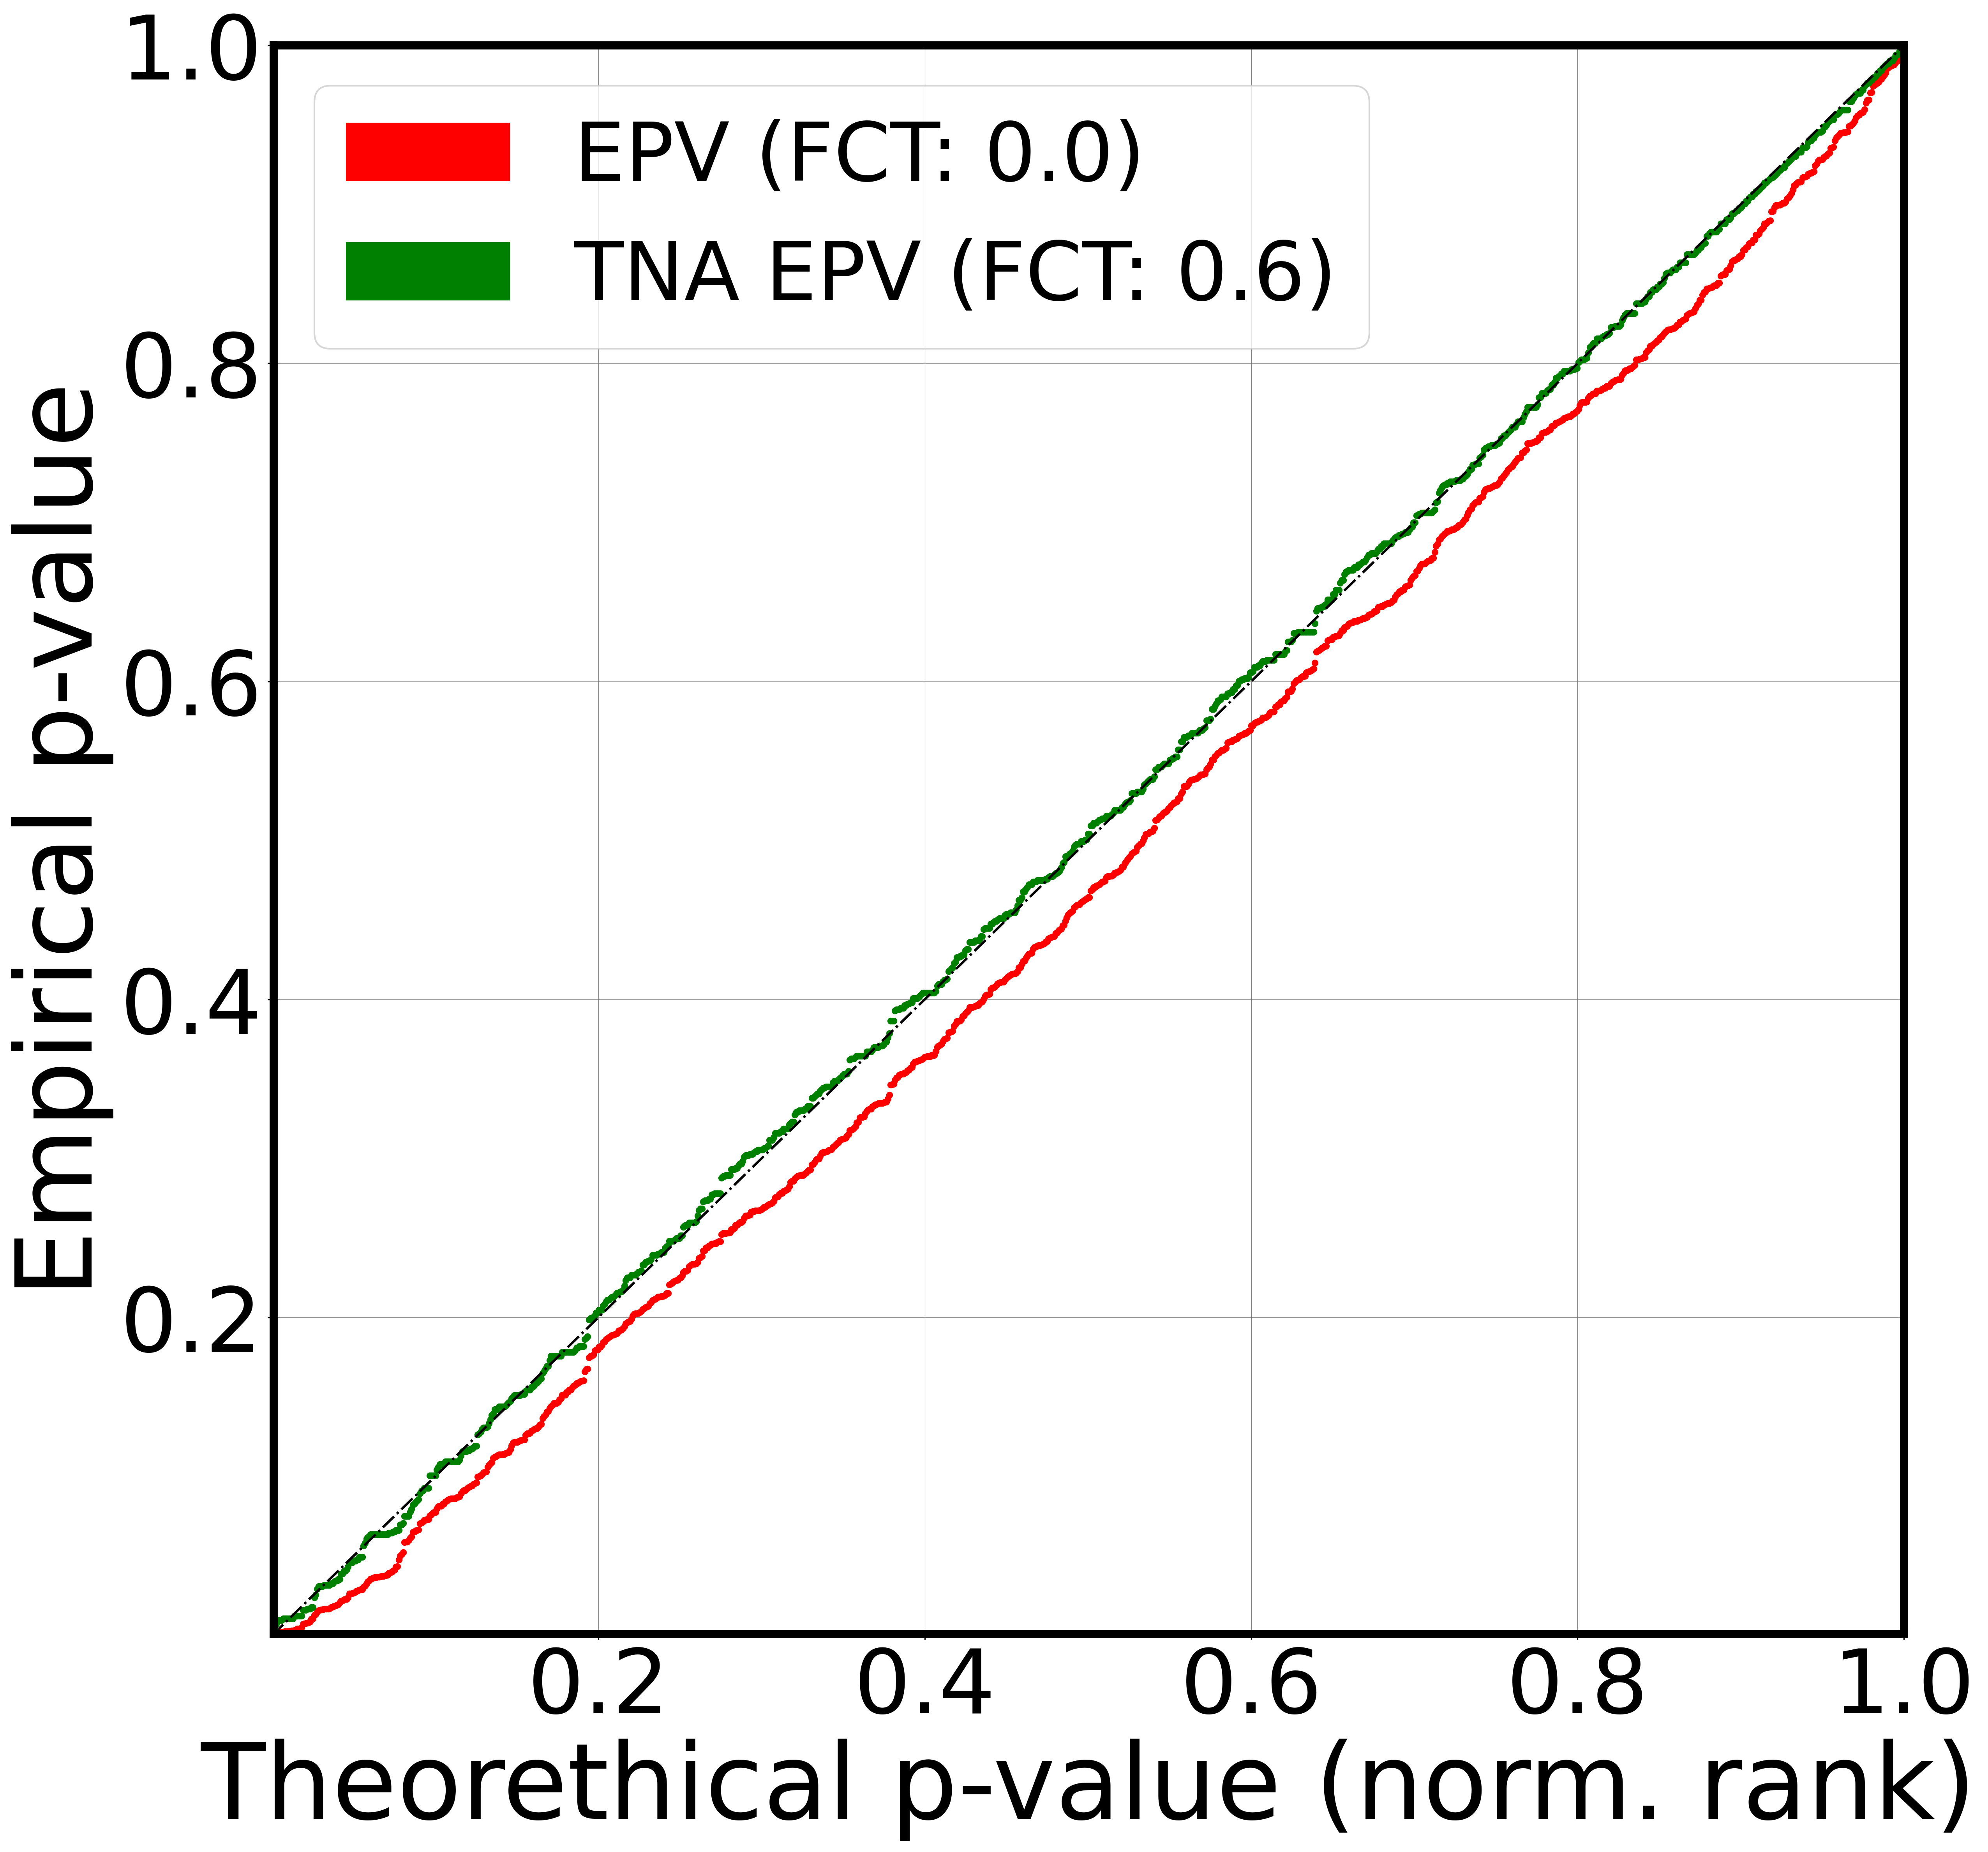
\includegraphics[width=1.7in]{img/cnn_QQ_balanced.png}&
%		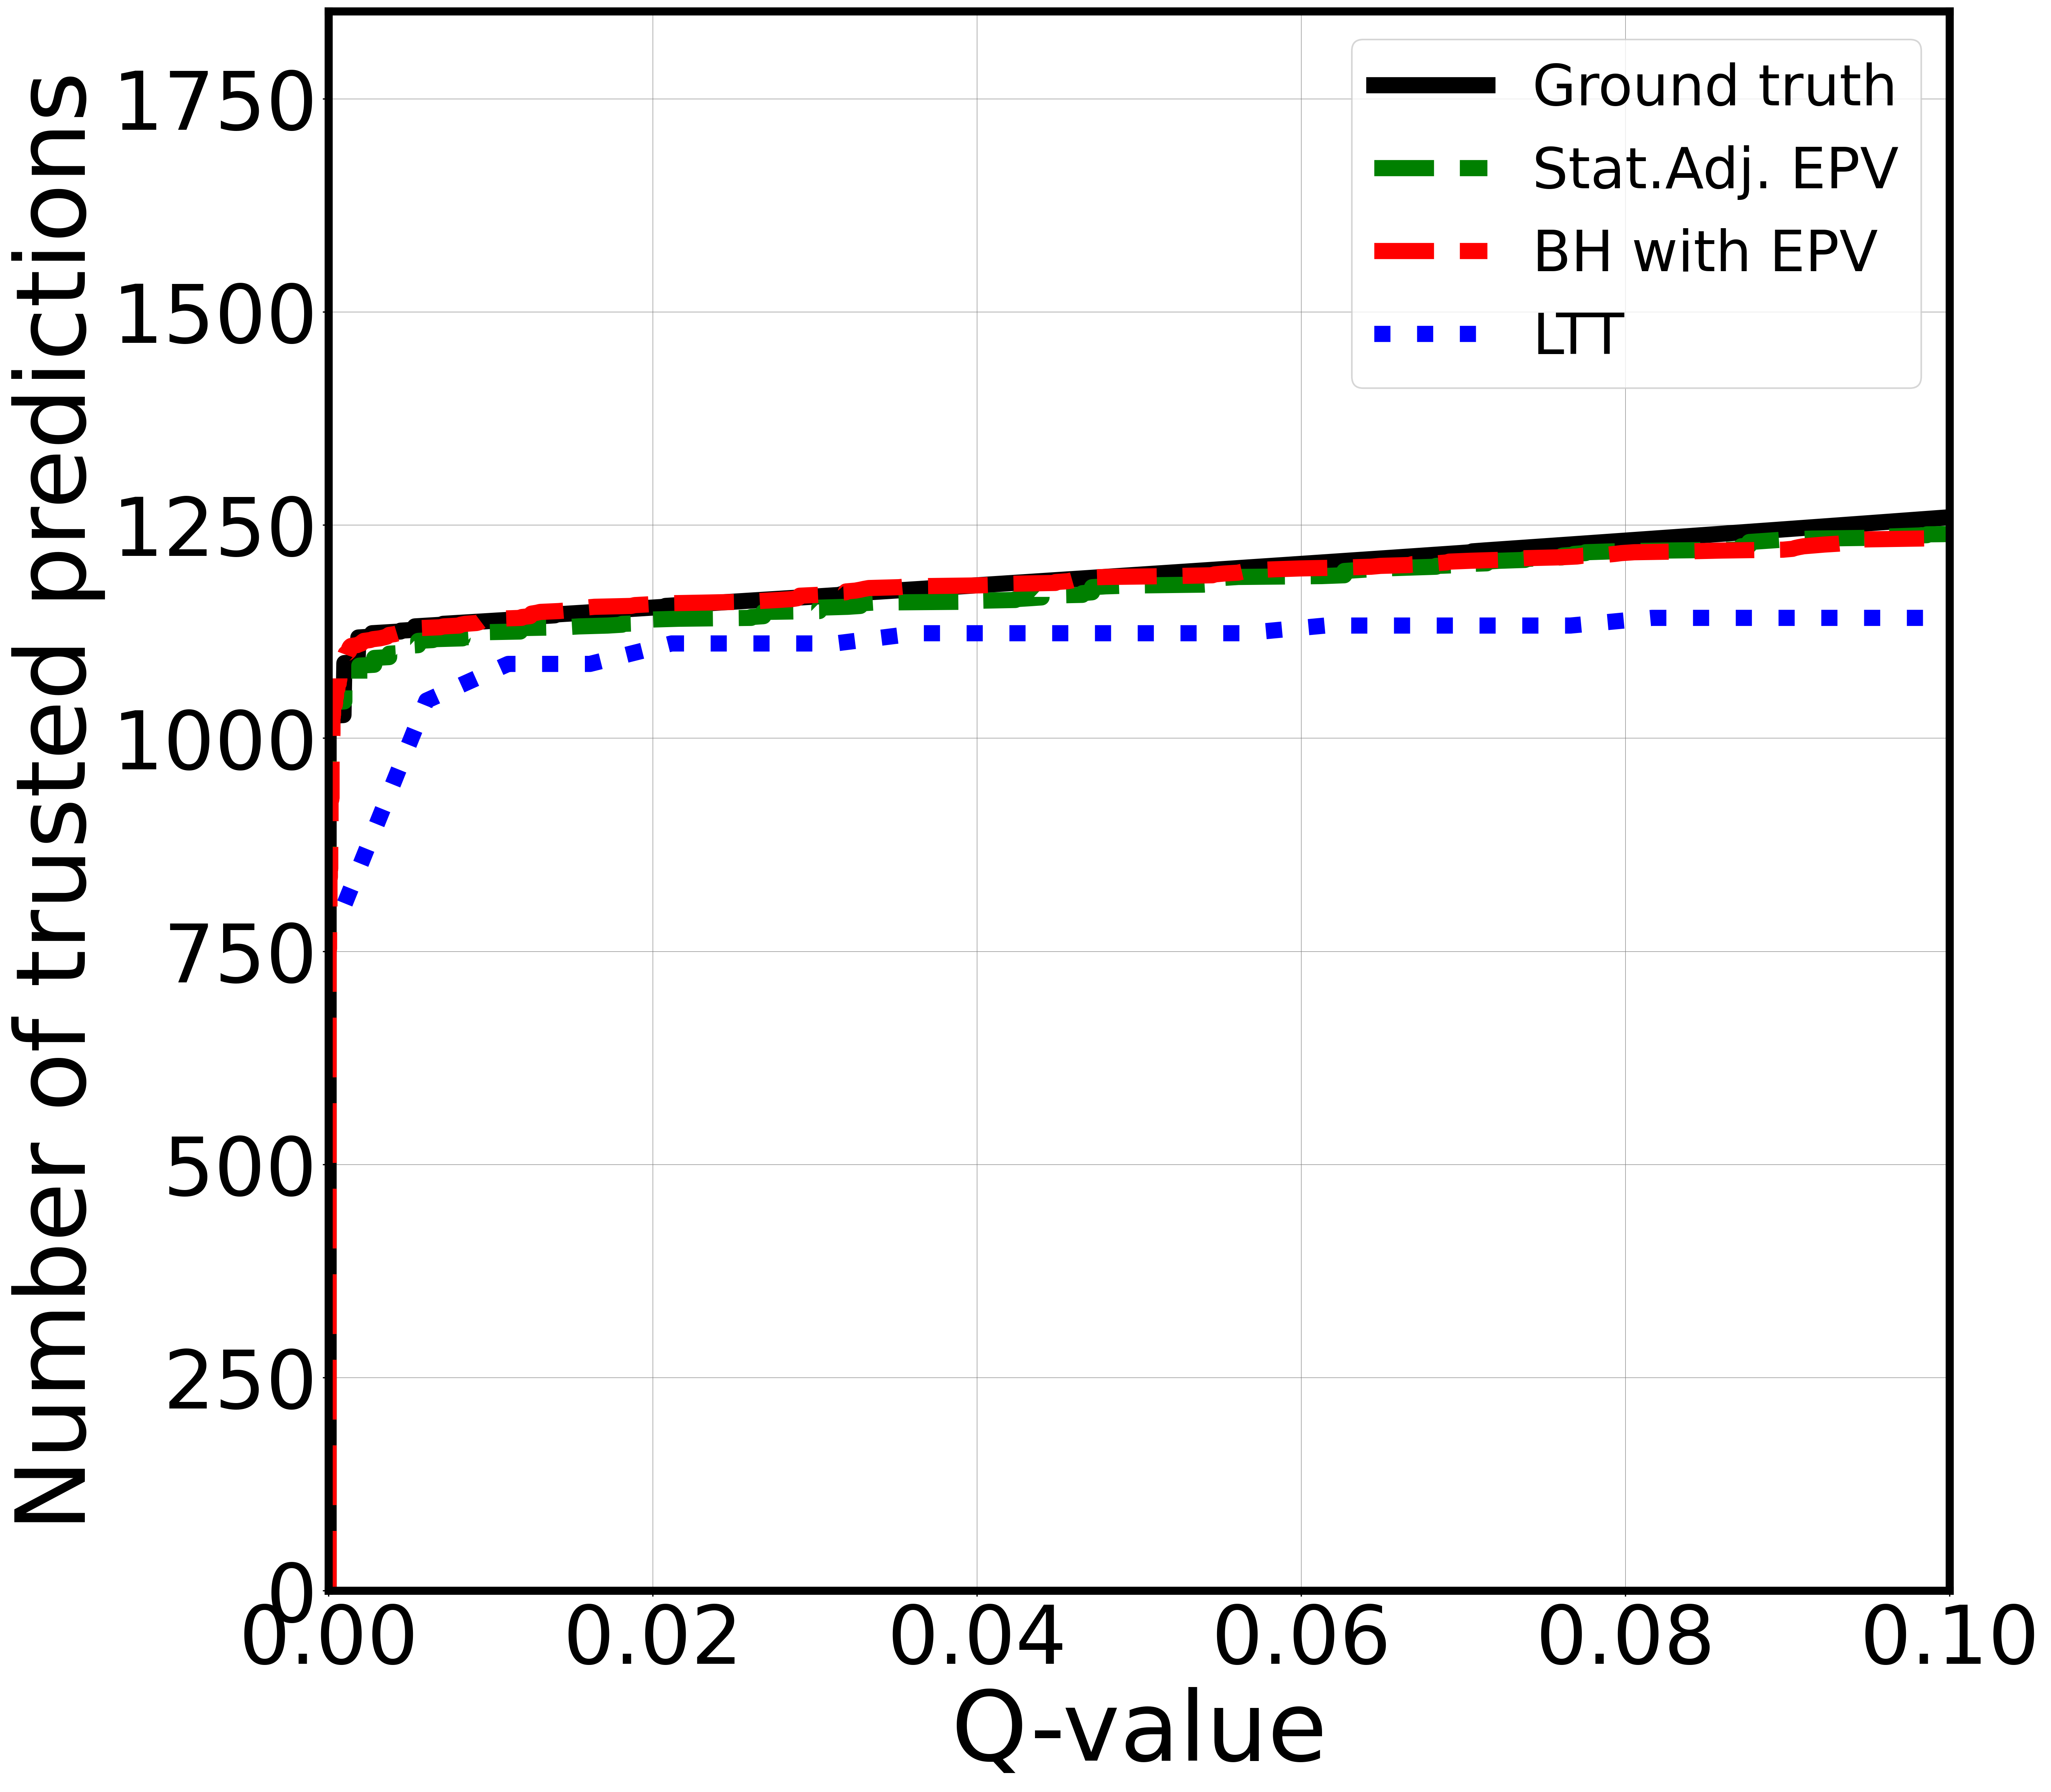
\includegraphics[width=1.7in]{img/cnn_balanced_fdr_control_loc.png} &
%		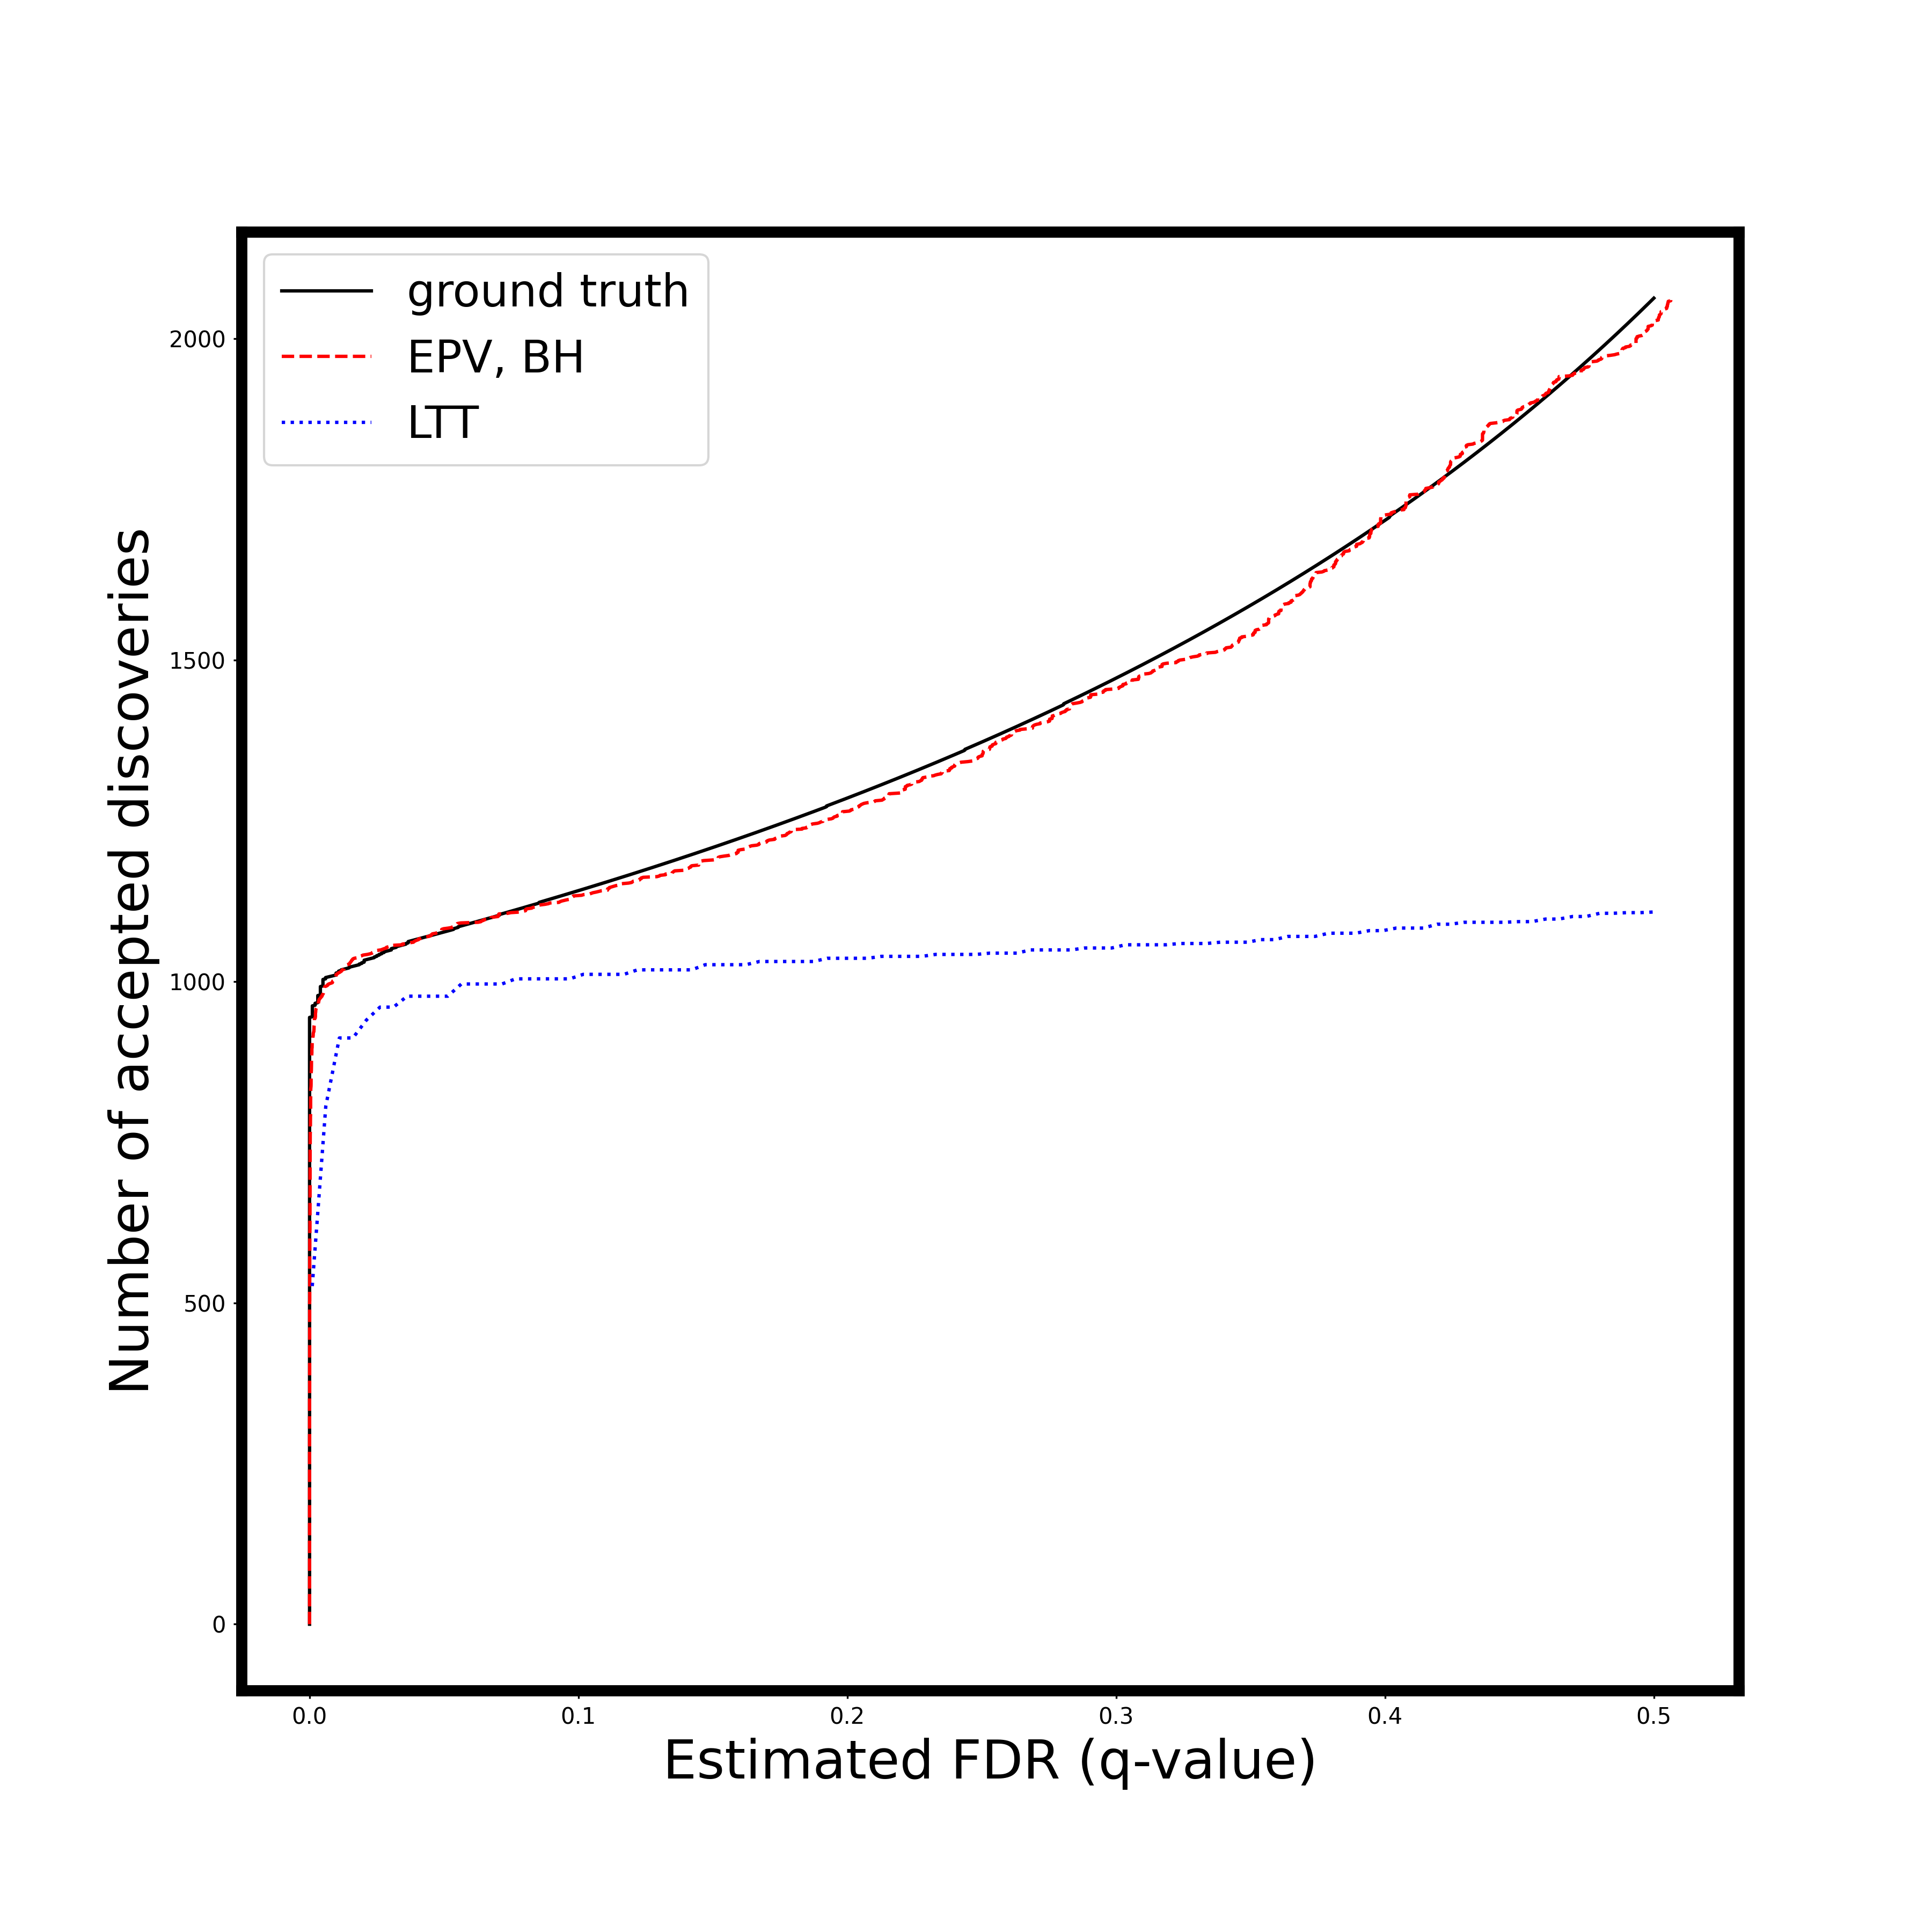
\includegraphics[width=1.7in]{img/cnn_balanced_fdr_control.png} & 
%		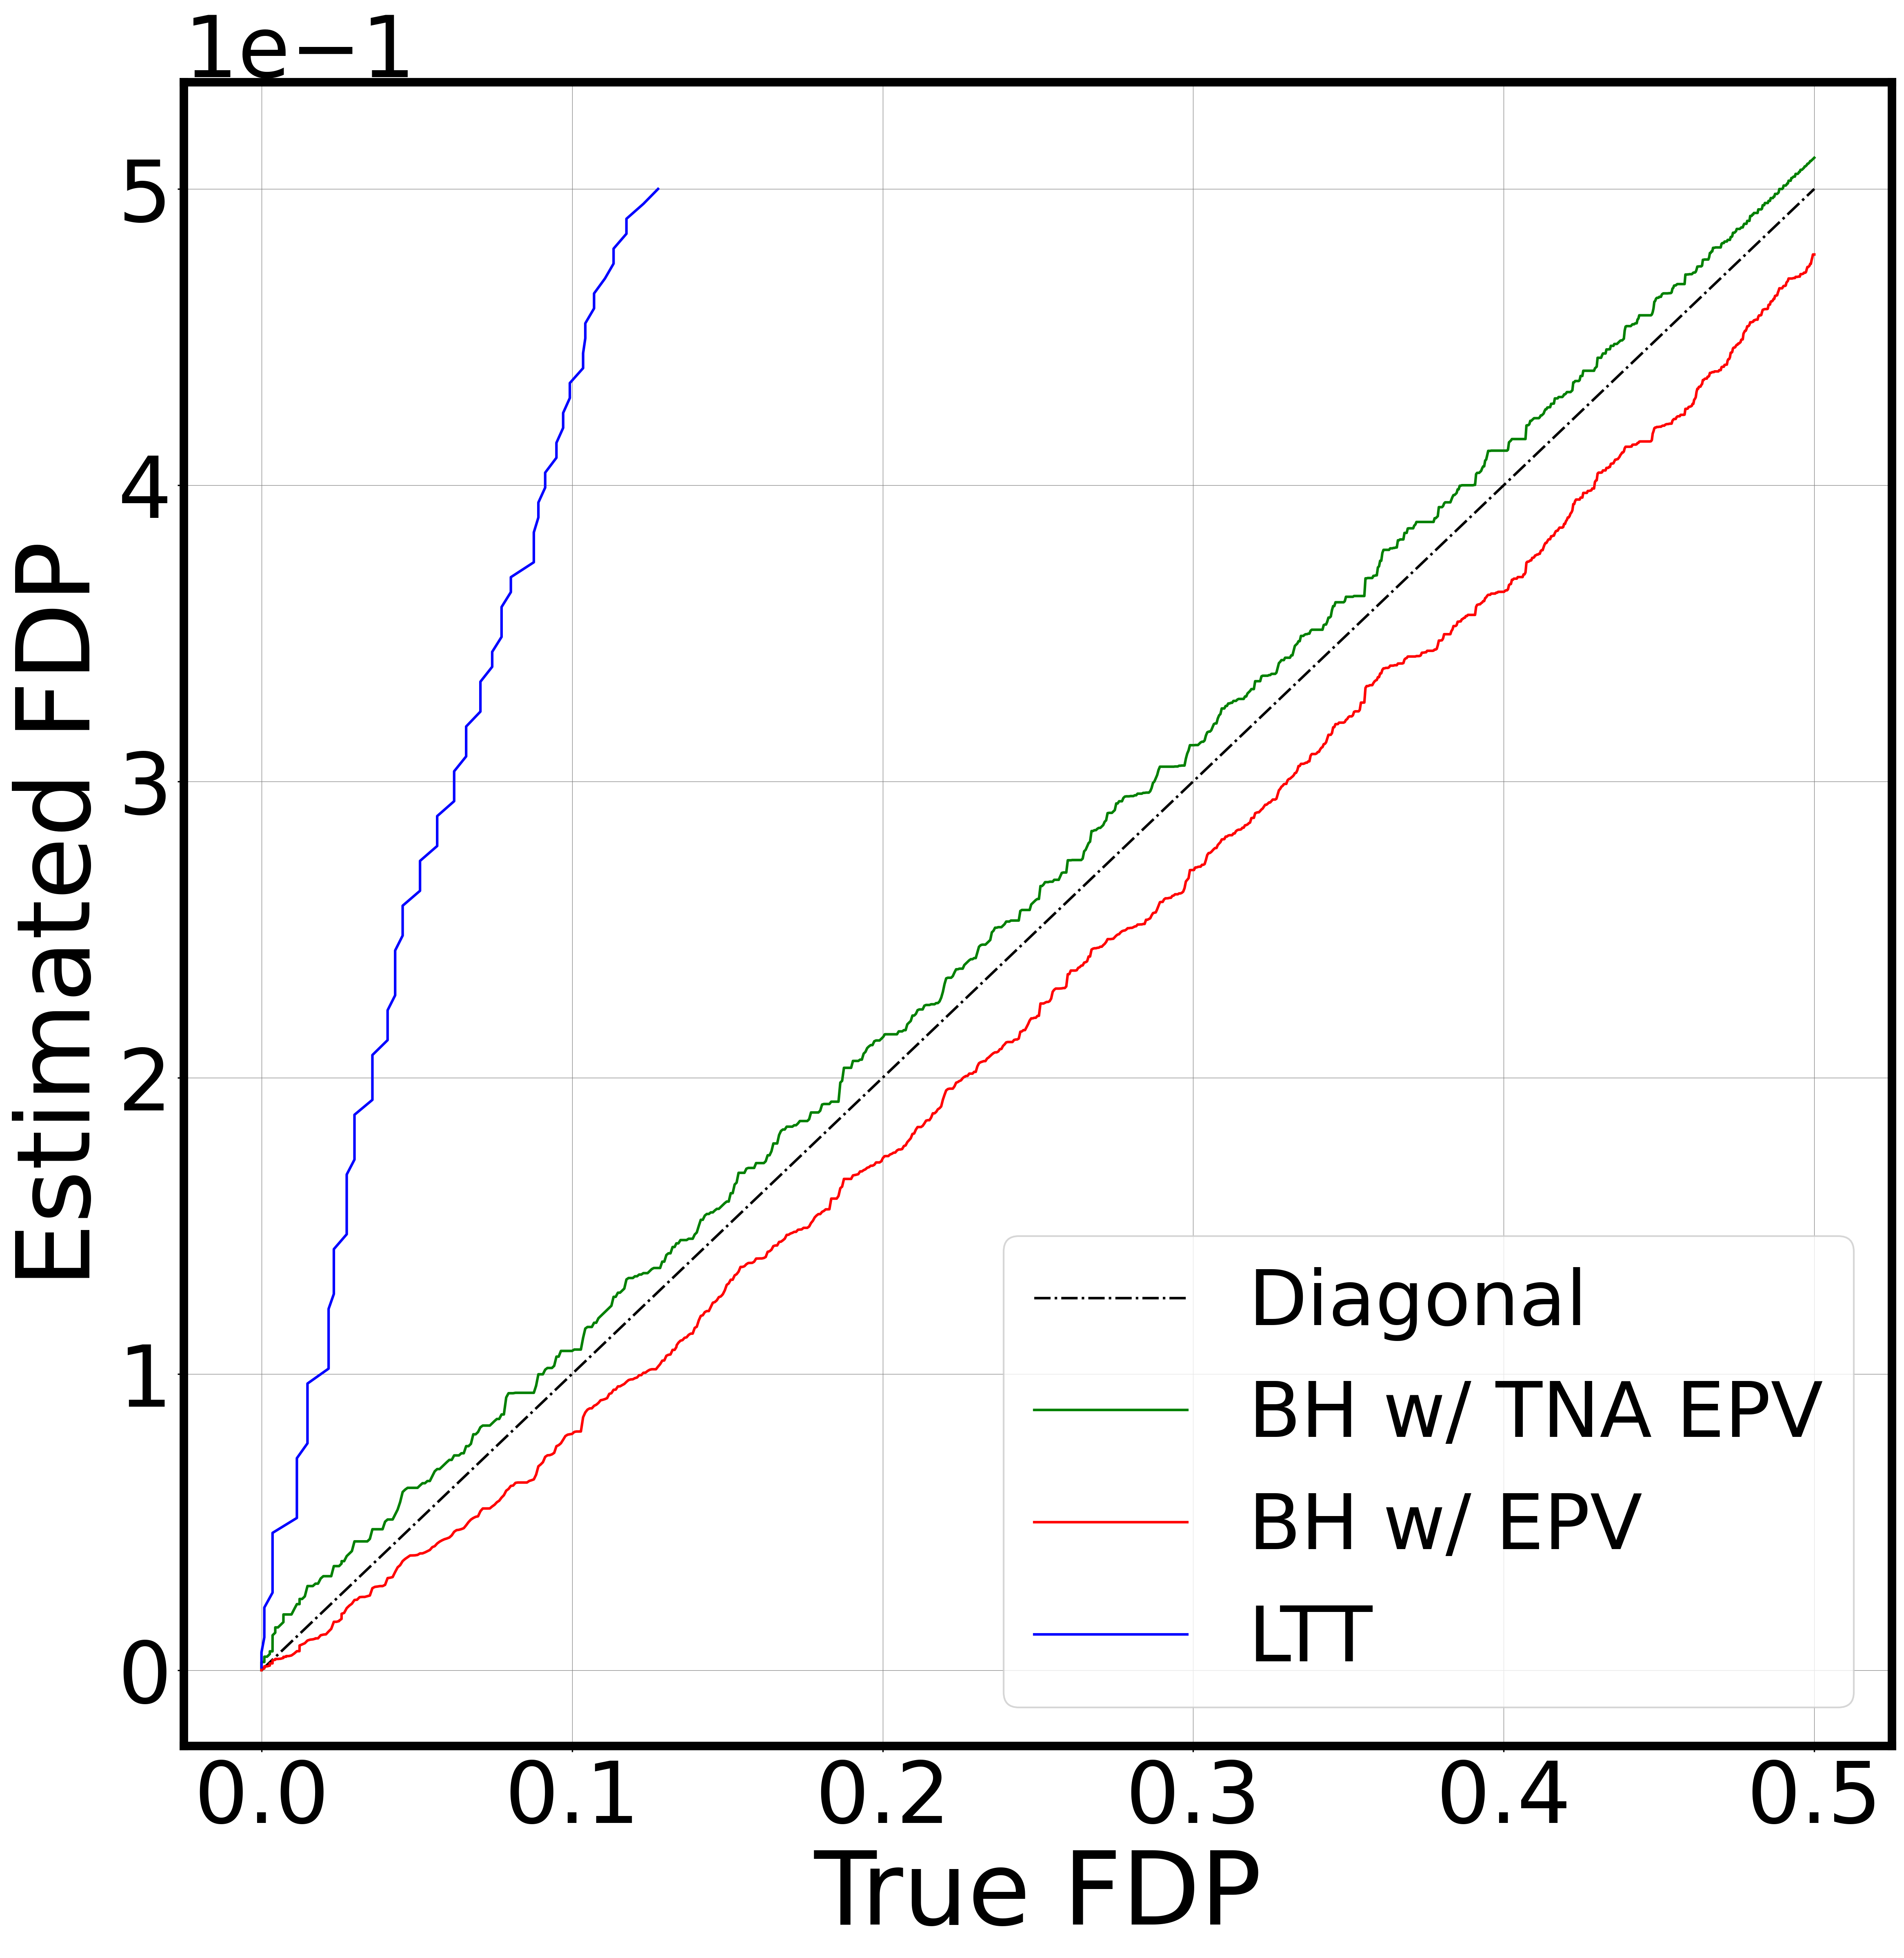
\includegraphics[width=1.7in]{img/cnn_FDPscat_balanced.png} \\		
%		A & B & C & D \\
%	\end{tabular}
%	\caption{{\bf  FDR control with EPV under altered class distribution shit.}
%		(A) QQ plot of the EPVs (red dots) and the EPVs with TNA (green dots) against the theoretical uniform distribution. The results of the Fisher's combination tests are indicated in the legend. (B) The number of accepted classifications as a function of the Q-values obtained with (i) ground truth (black line), (ii) BH with EPV (red), (iii) BH with EPV with TNA (green), and (iv) LTT (blue). (C) Same as (B) with over the entire Q-value range. (D) Deviation of the estimated FDR from the actual FDR obtained with (i) BH with EPV (red line), (ii) BH with EPV and TNA (green line), (iii) LTT (blue line).}
%	\label{fig:mnist_rebalance}
%\end{figure}

\section{Experimental results}

\subsection{PCam: tumor classification}



The PatchCamelyon (PCam) benchmark dataset is a collection of histopathologic scans of lymph node sections \cite{Veeling2018-qh} derived from the Camelyon 16 challenge \cite{camelyon16}. PCam consists of 327,680 colored images of size 96x96 each. The challenge is to identify the presence (positive) or absence (negative) of any histopathology. The dataset creators of PCam underline that all the positive and negative instances in the training, validation, test sets are equally distributed, resulting in a class balance of 50:50\%; while the positive and negative class balance in the Camelyon 16 test dataset is 31\% :69\%. Therefore,  the actual true class proportions in PCcam might be significantly different in real-life applications, making the FDR control with methods like LTT inaccurate in practical applications. We manually resampled the test data sets of the PCam so that the class ratios become the same as of the Camelyon 16 dataset, because,  in our opinion,  this class ratio is probably more realistic for real life scenarios. We used the trained resnet34-pcam model, which is a popular, deep residual network from the TIA (Tissue Image Analysis) toolbox \cite{Pocock2022} with an overall f1-score of 0.889, as stated by the authors.


\begin{figure}[h!]
	\centering
	\begin{tabular}{cccc}
 		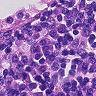
\includegraphics[width=1.in]{img/pcam1.jpg} &
		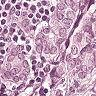
\includegraphics[width=1.in]{img/pcam2.jpg} & 
            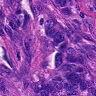
\includegraphics[width=1.in]{img/pcam3.jpg} &
             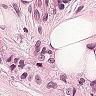
\includegraphics[width=1.in]{img/pcam4.jpg}
        \end{tabular}
	\caption{{\bf Instances of PCam dataset.}}
	\label{fig:pcam_example}
\end{figure} 


The evaluation of FDR controlling methods on the PCam dataset is shown in the Figure \ref{fig:pcam} with original class distribution. The plots indicate that all three FDR control methods are fairly accurate in practice. Perhaps, the QQ plots of the test EPVs (red dots) and the test NTA EPVs (green dots) in the Figure \ref{fig:pcam}A indicate that the test p-values are slightly biased; however, the NSA method manages to reduce this bias in the EPVs. This indicates a slight overfitting and/or distribution shifts between the training and test data sets. However, when we changed the even class distribution to 31\%:69\%, the LTT FDR control method resulted in liberal FDR control, the BH protocol with standard EPVs resulted in conservative FDR control; whereas, the BH with the TNA EPVs resulted in accurate FDR control,  especially at critical $\alpha$ levels (0-0.1). These results are shown in the Figure \ref{fig:pcam_rebalance}.


%
%
%\begin{figure}
%
%	\begin{tabular}{cccc}
% 		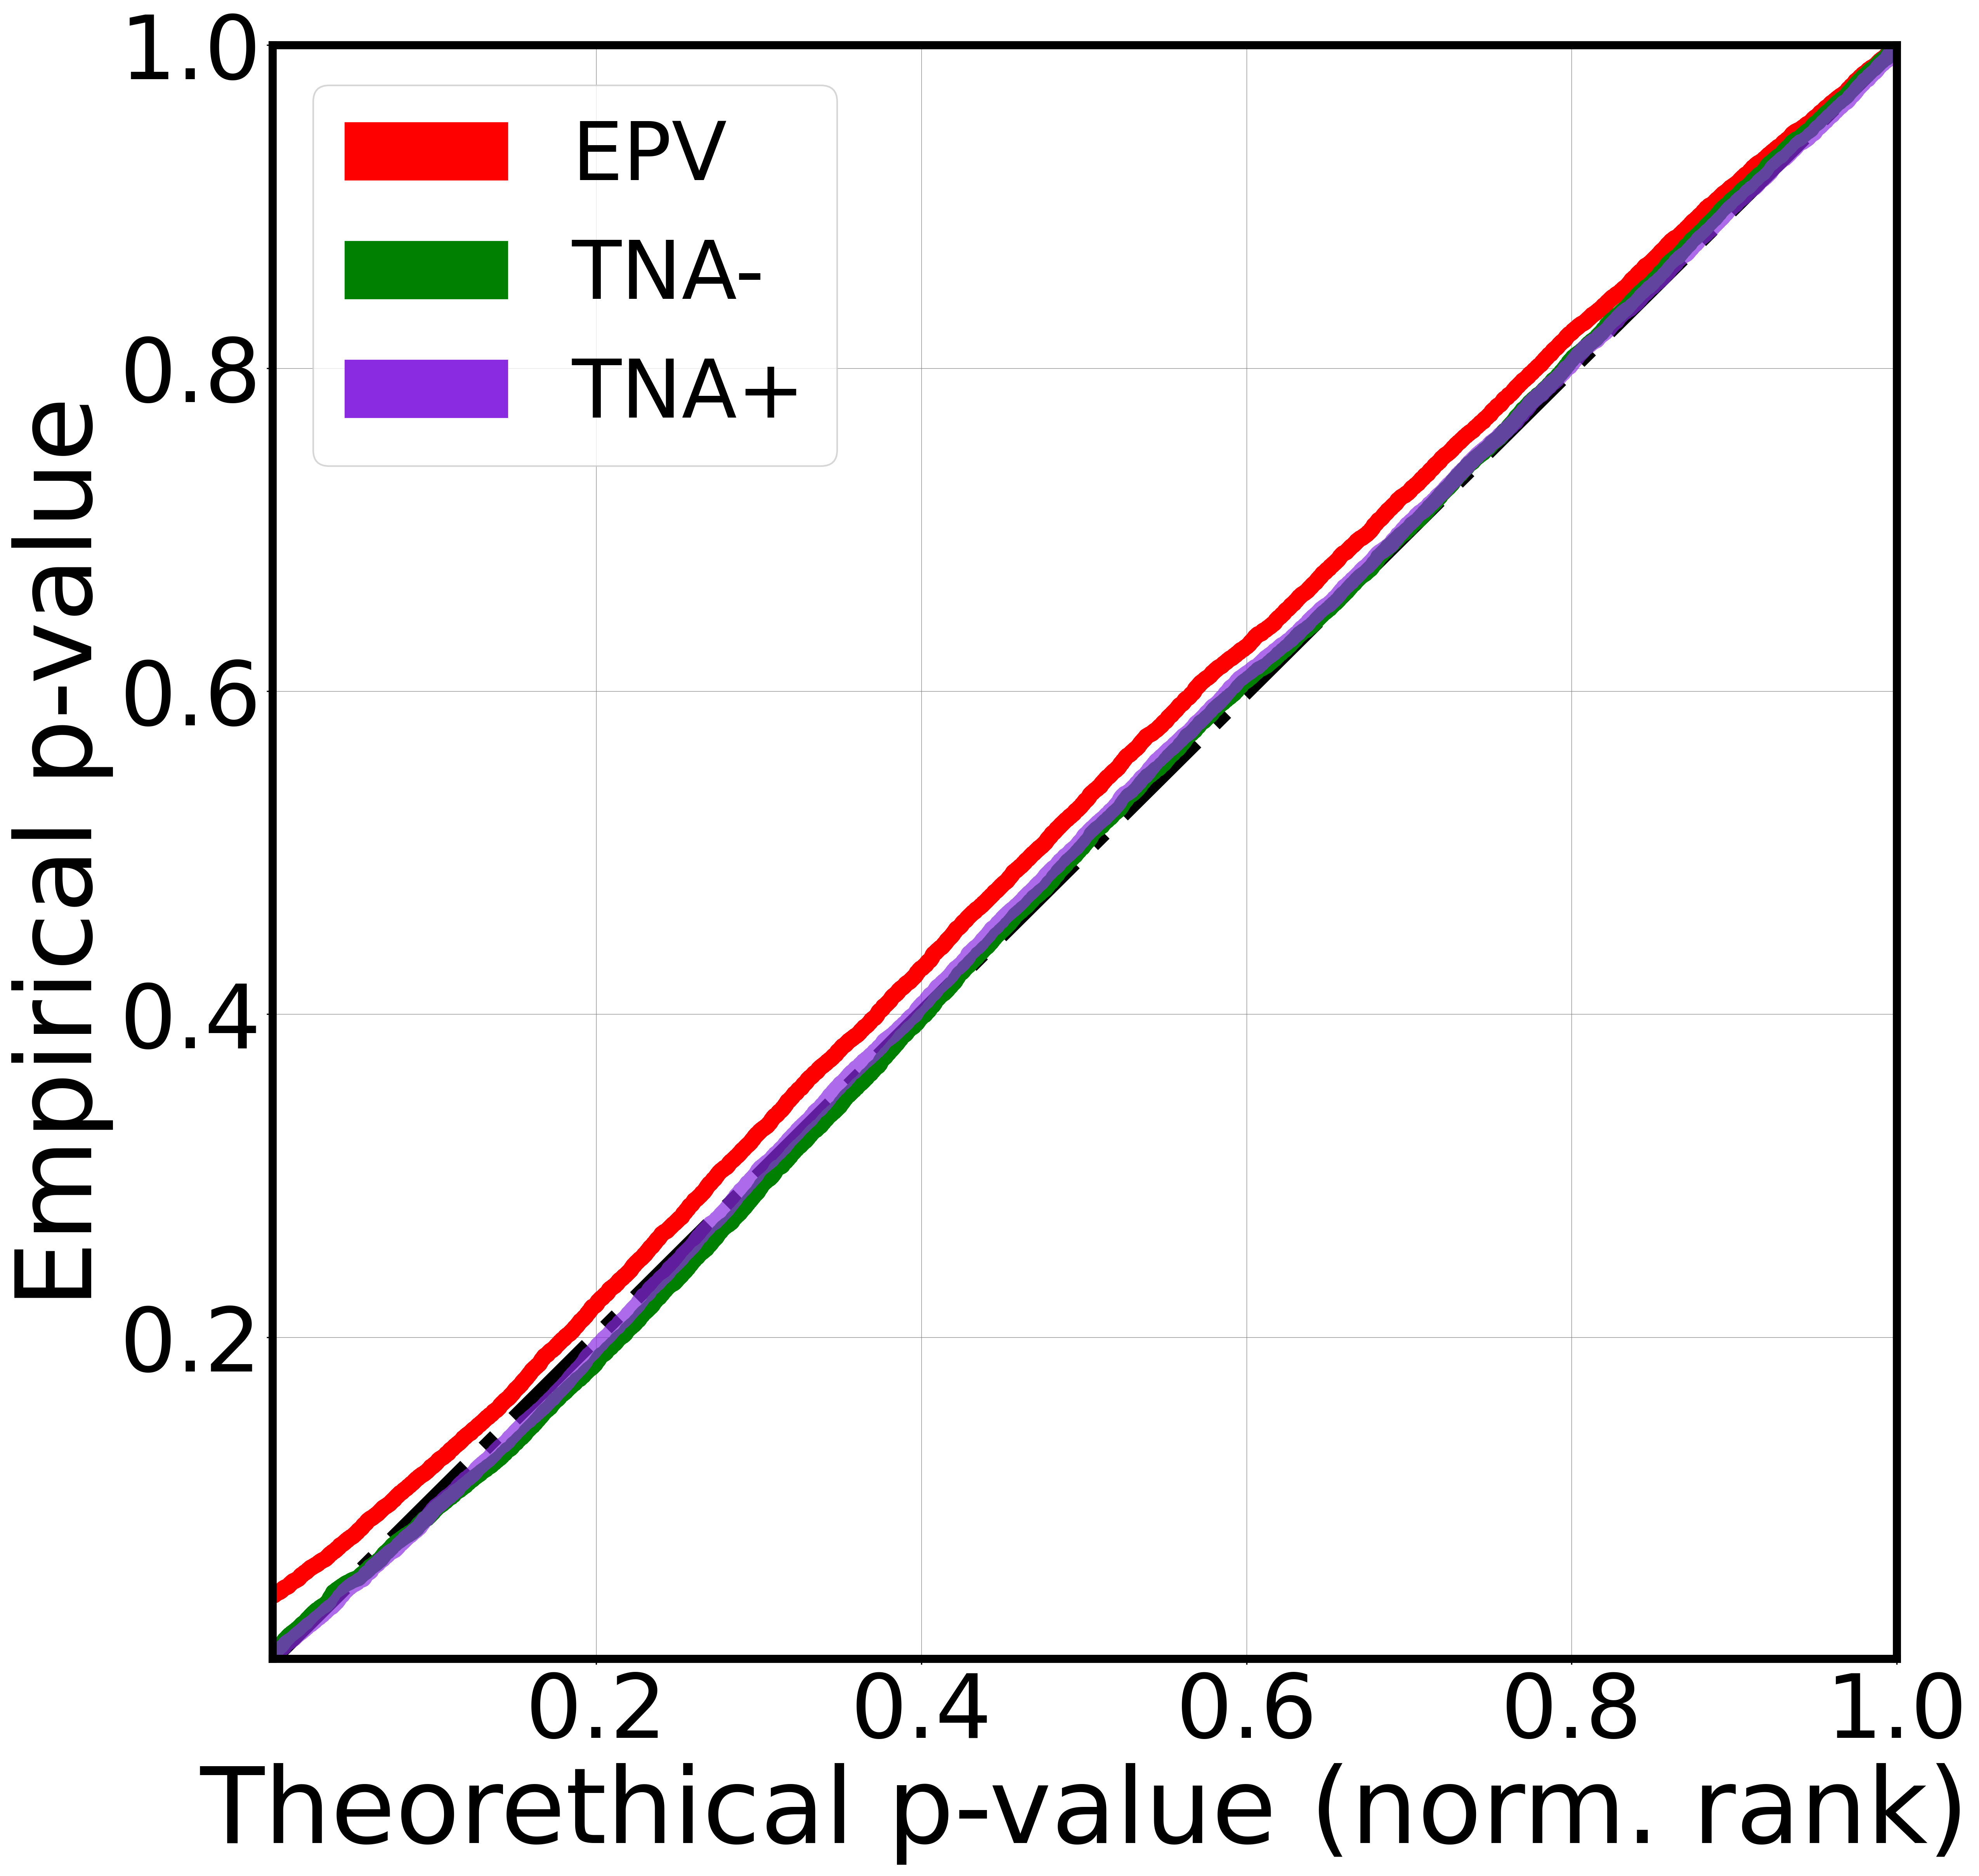
\includegraphics[width=1.7in]{img/cnn_QQ_pcam_balanced.png} &
%		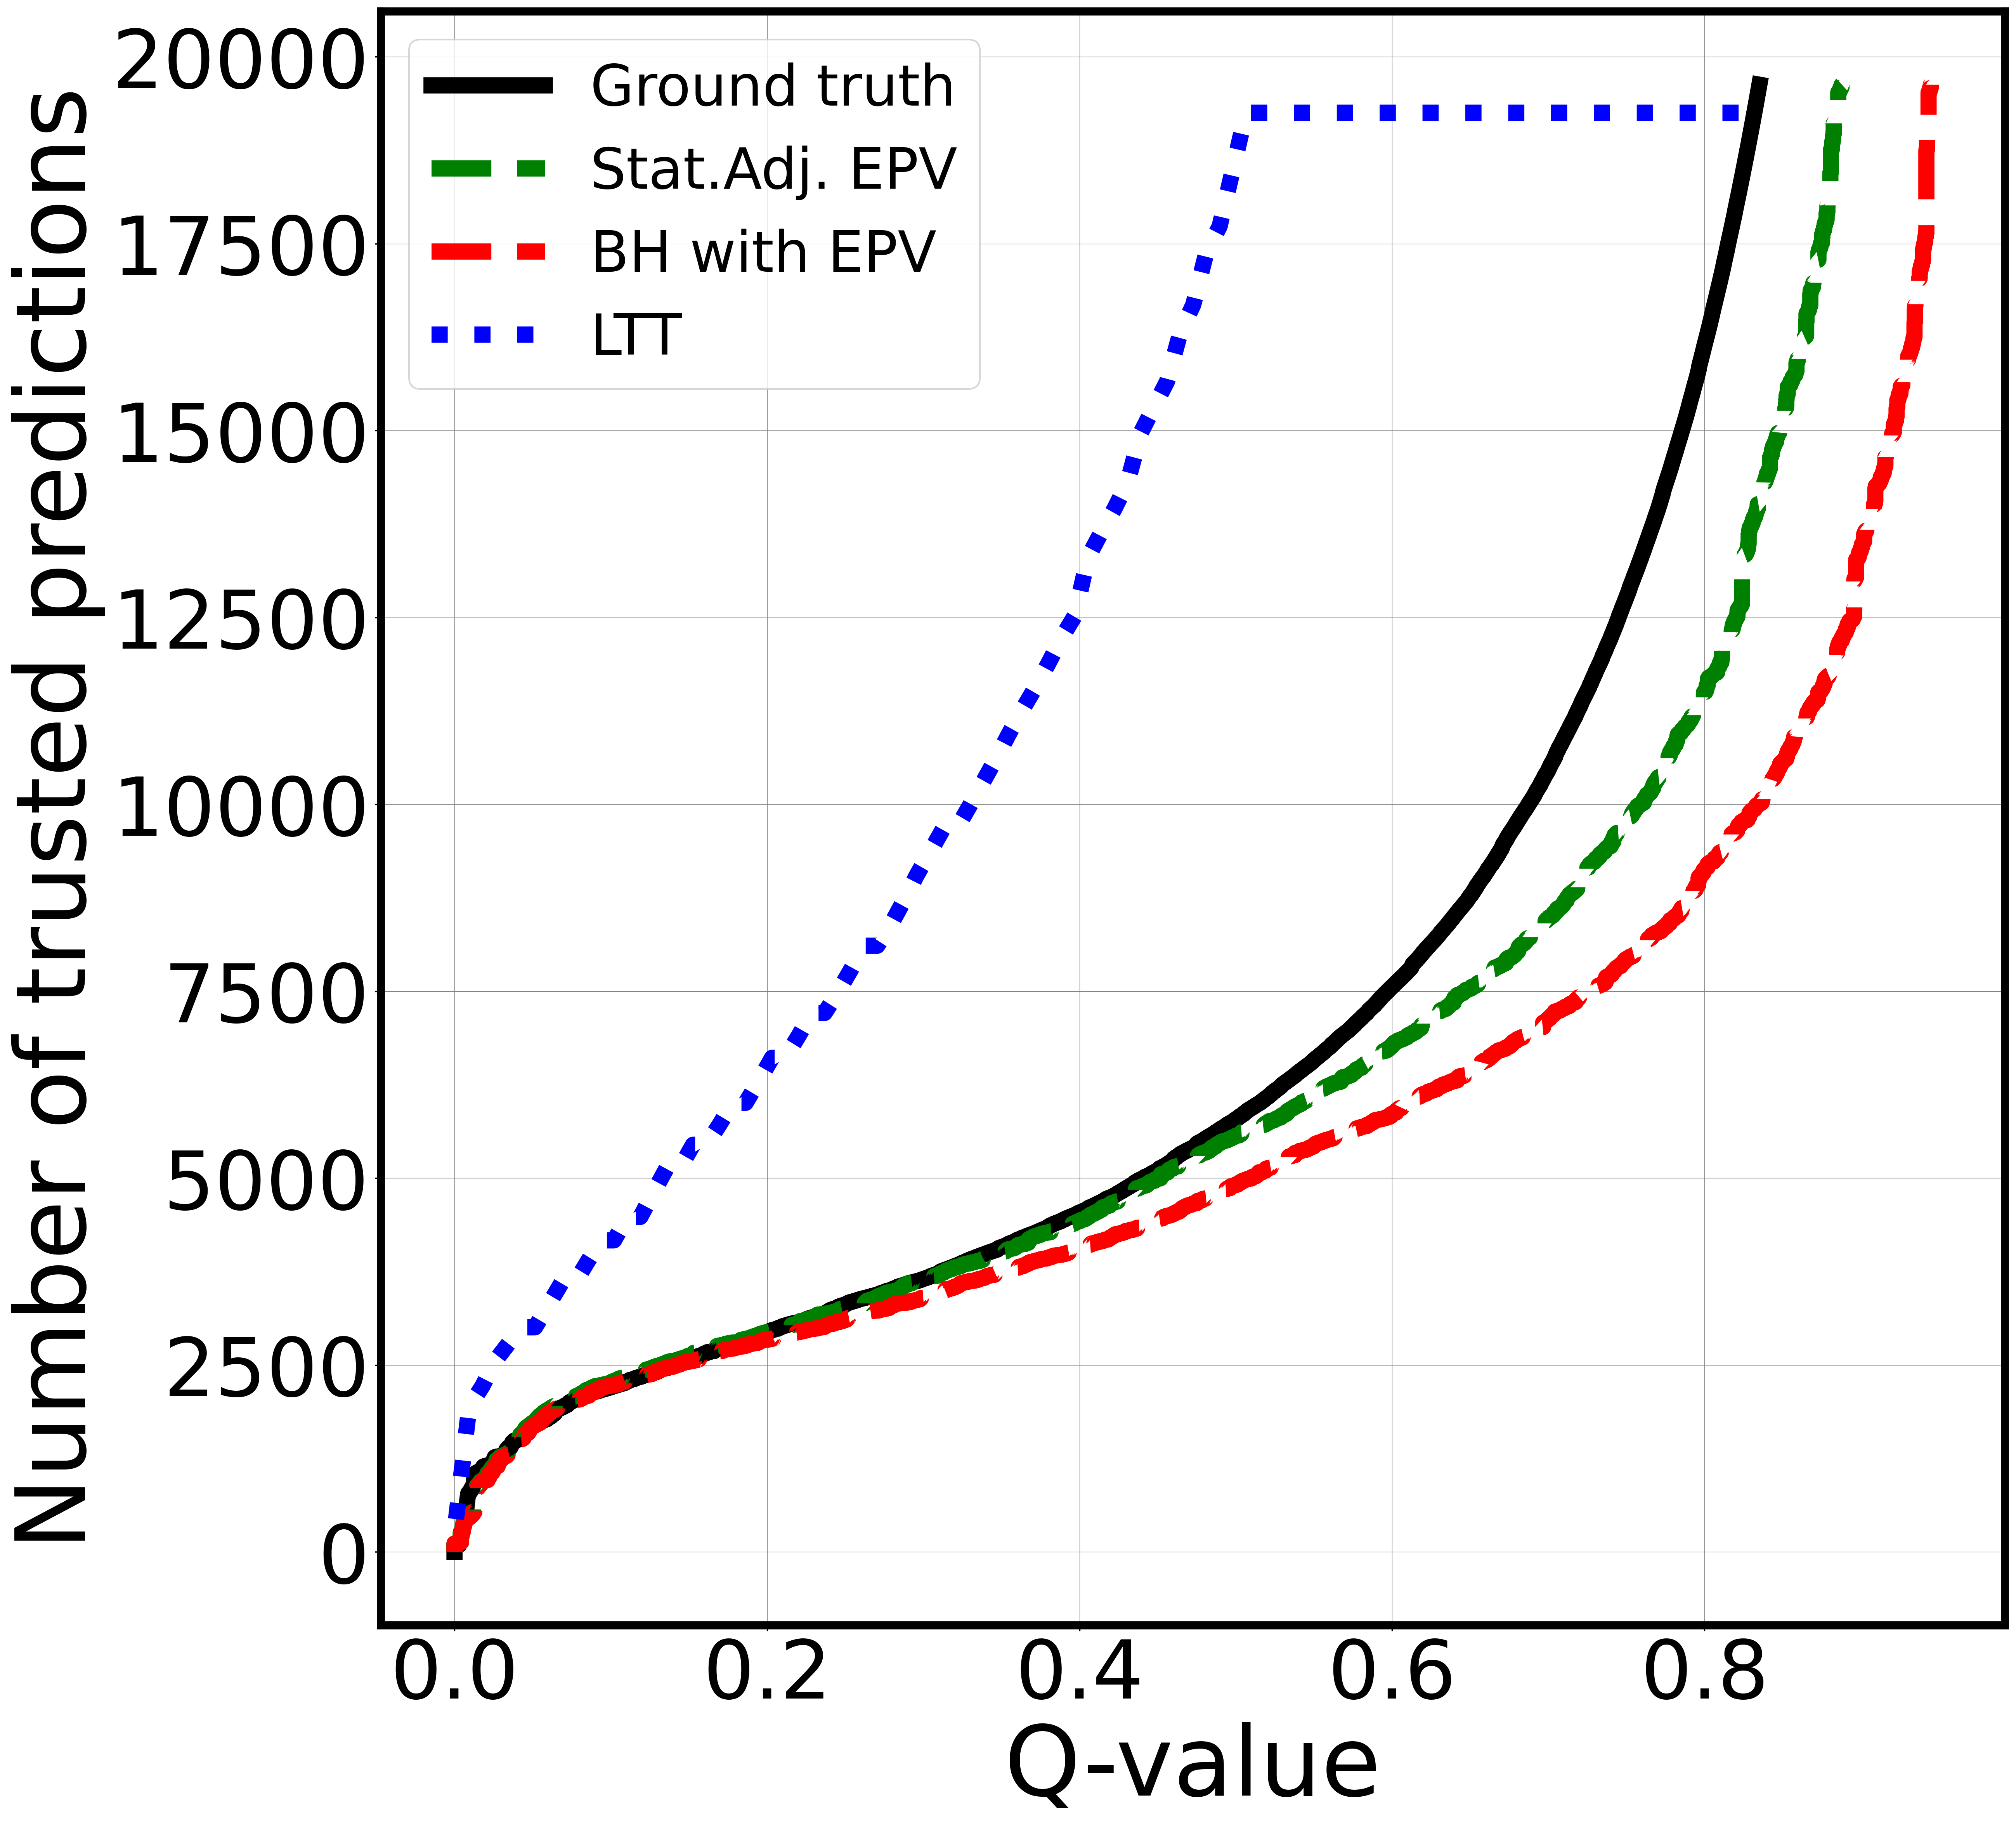
\includegraphics[width=1.7in]{img/cnn_pcam_balanced_fdr_control.png} & 
%        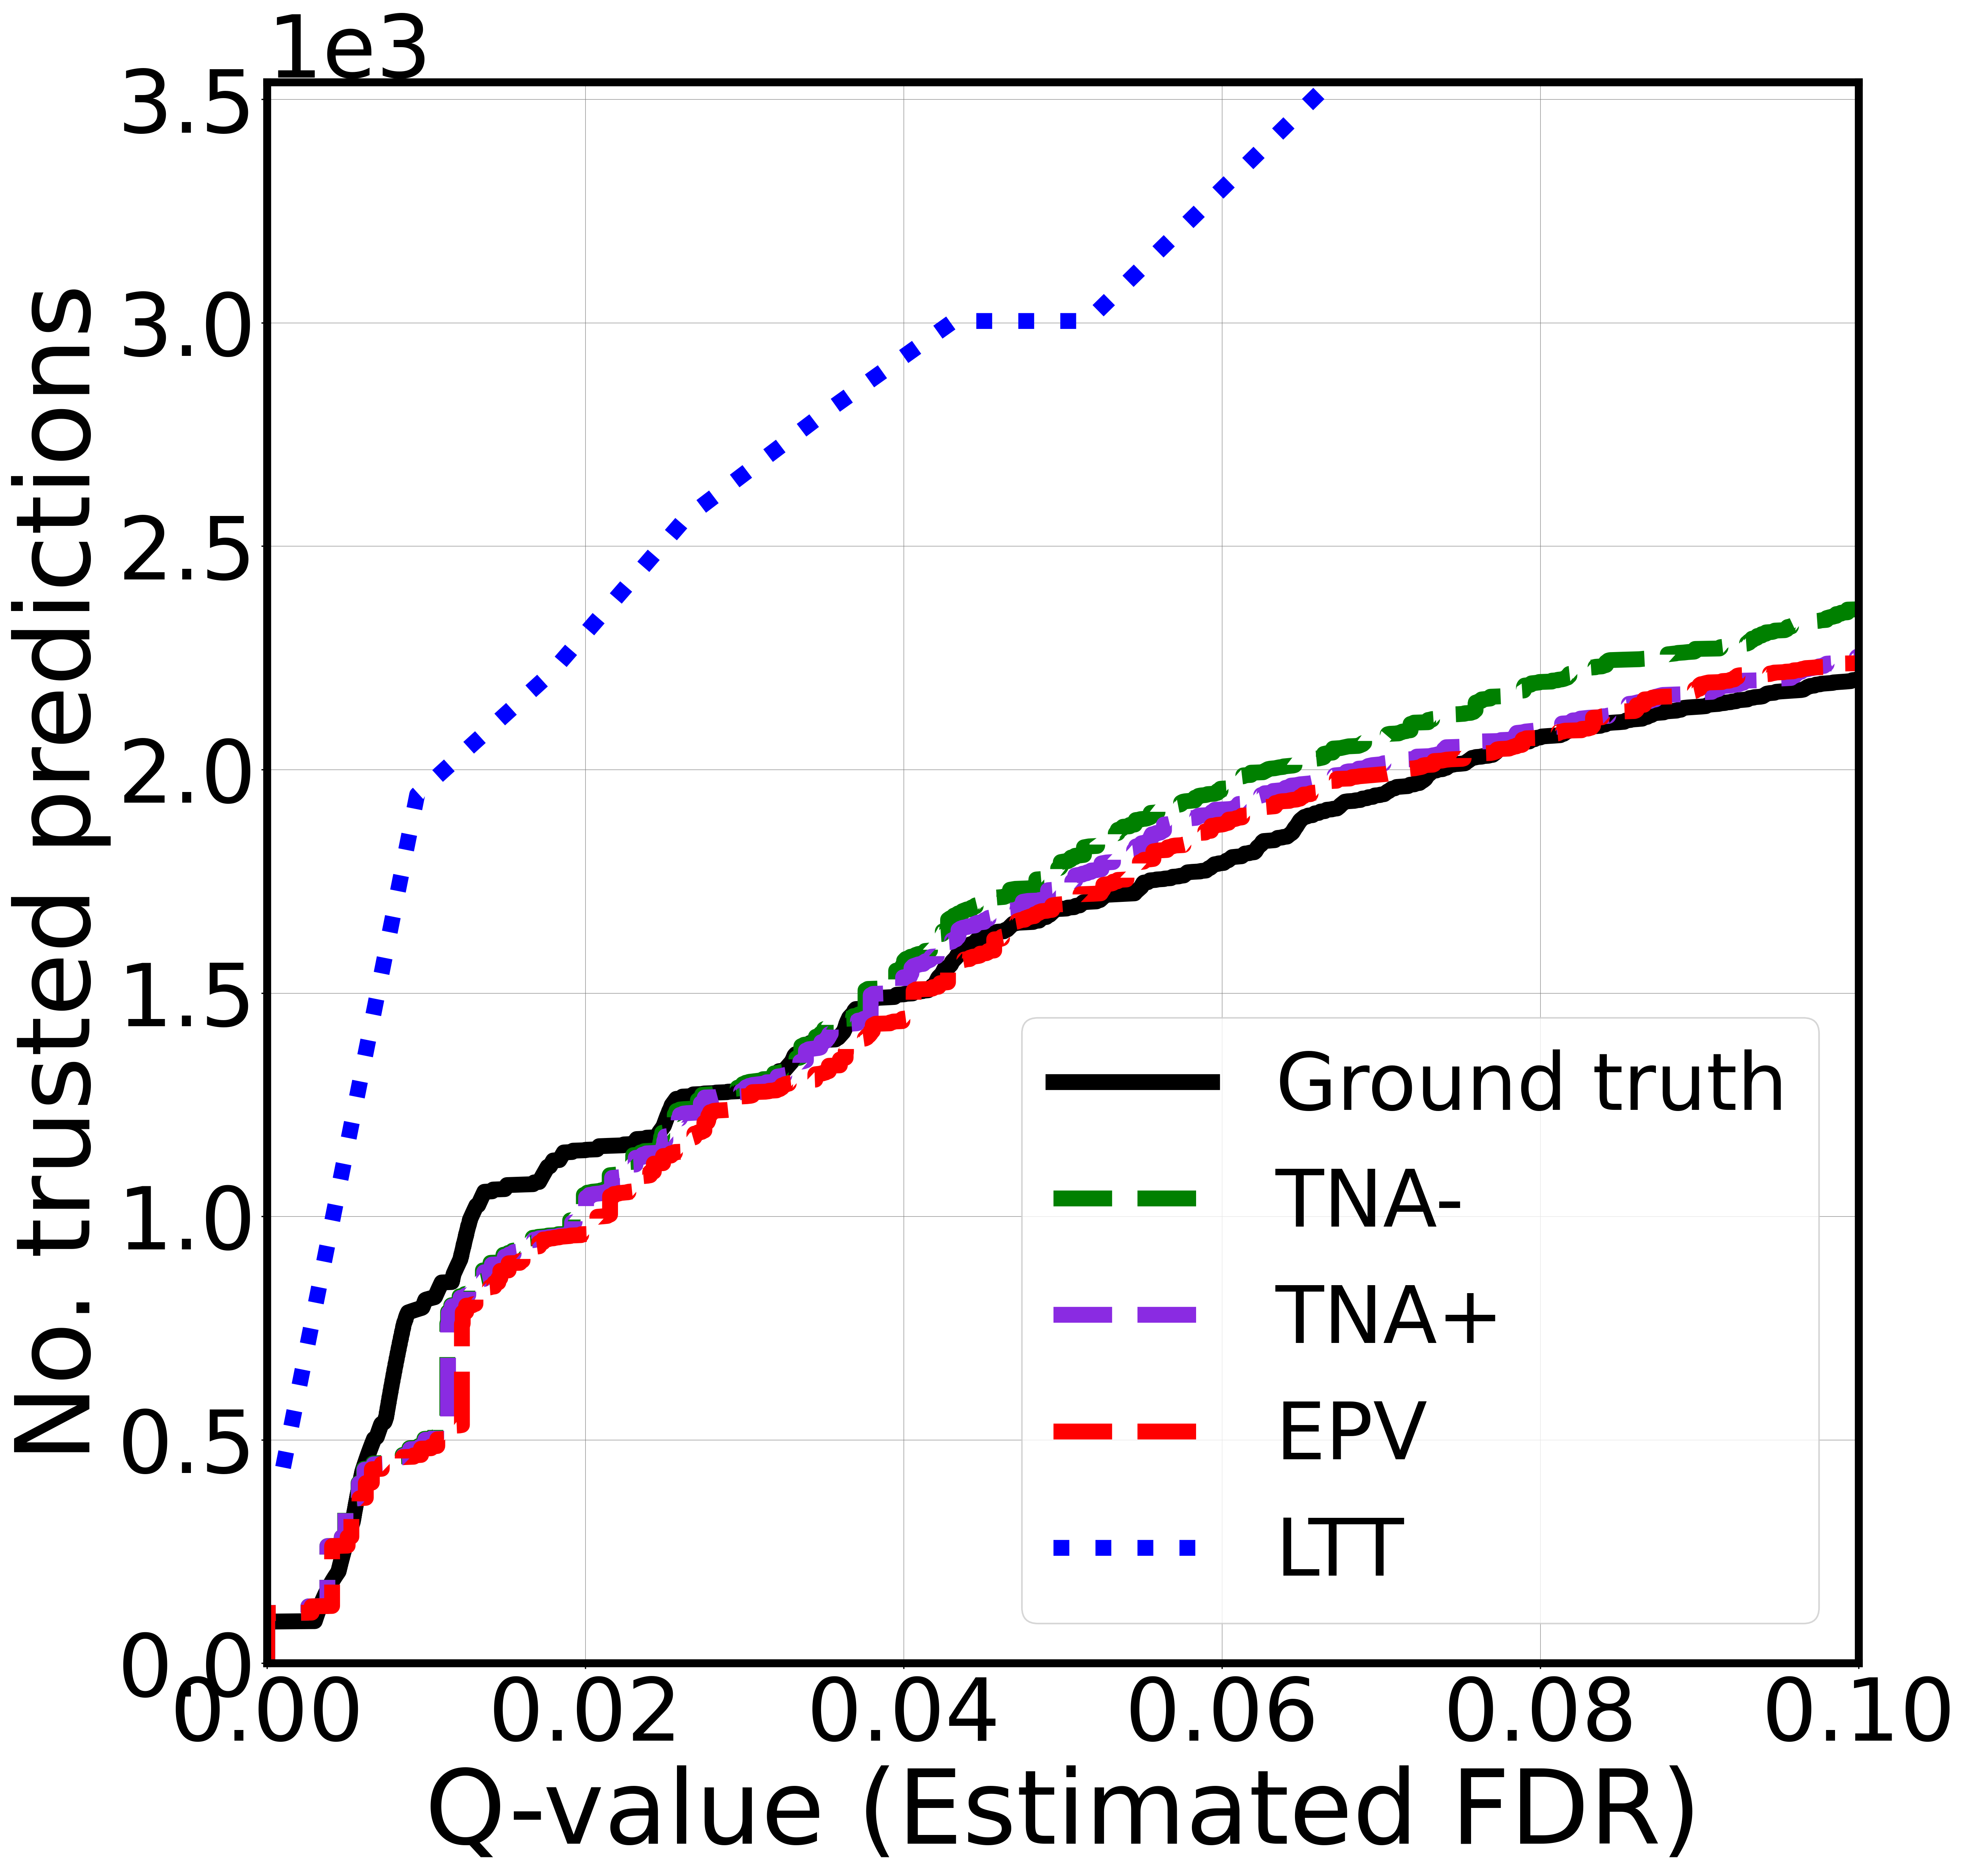
\includegraphics[width=1.7in]{img/cnn_pcam_balanced_fdr_control_loc.png} &
%        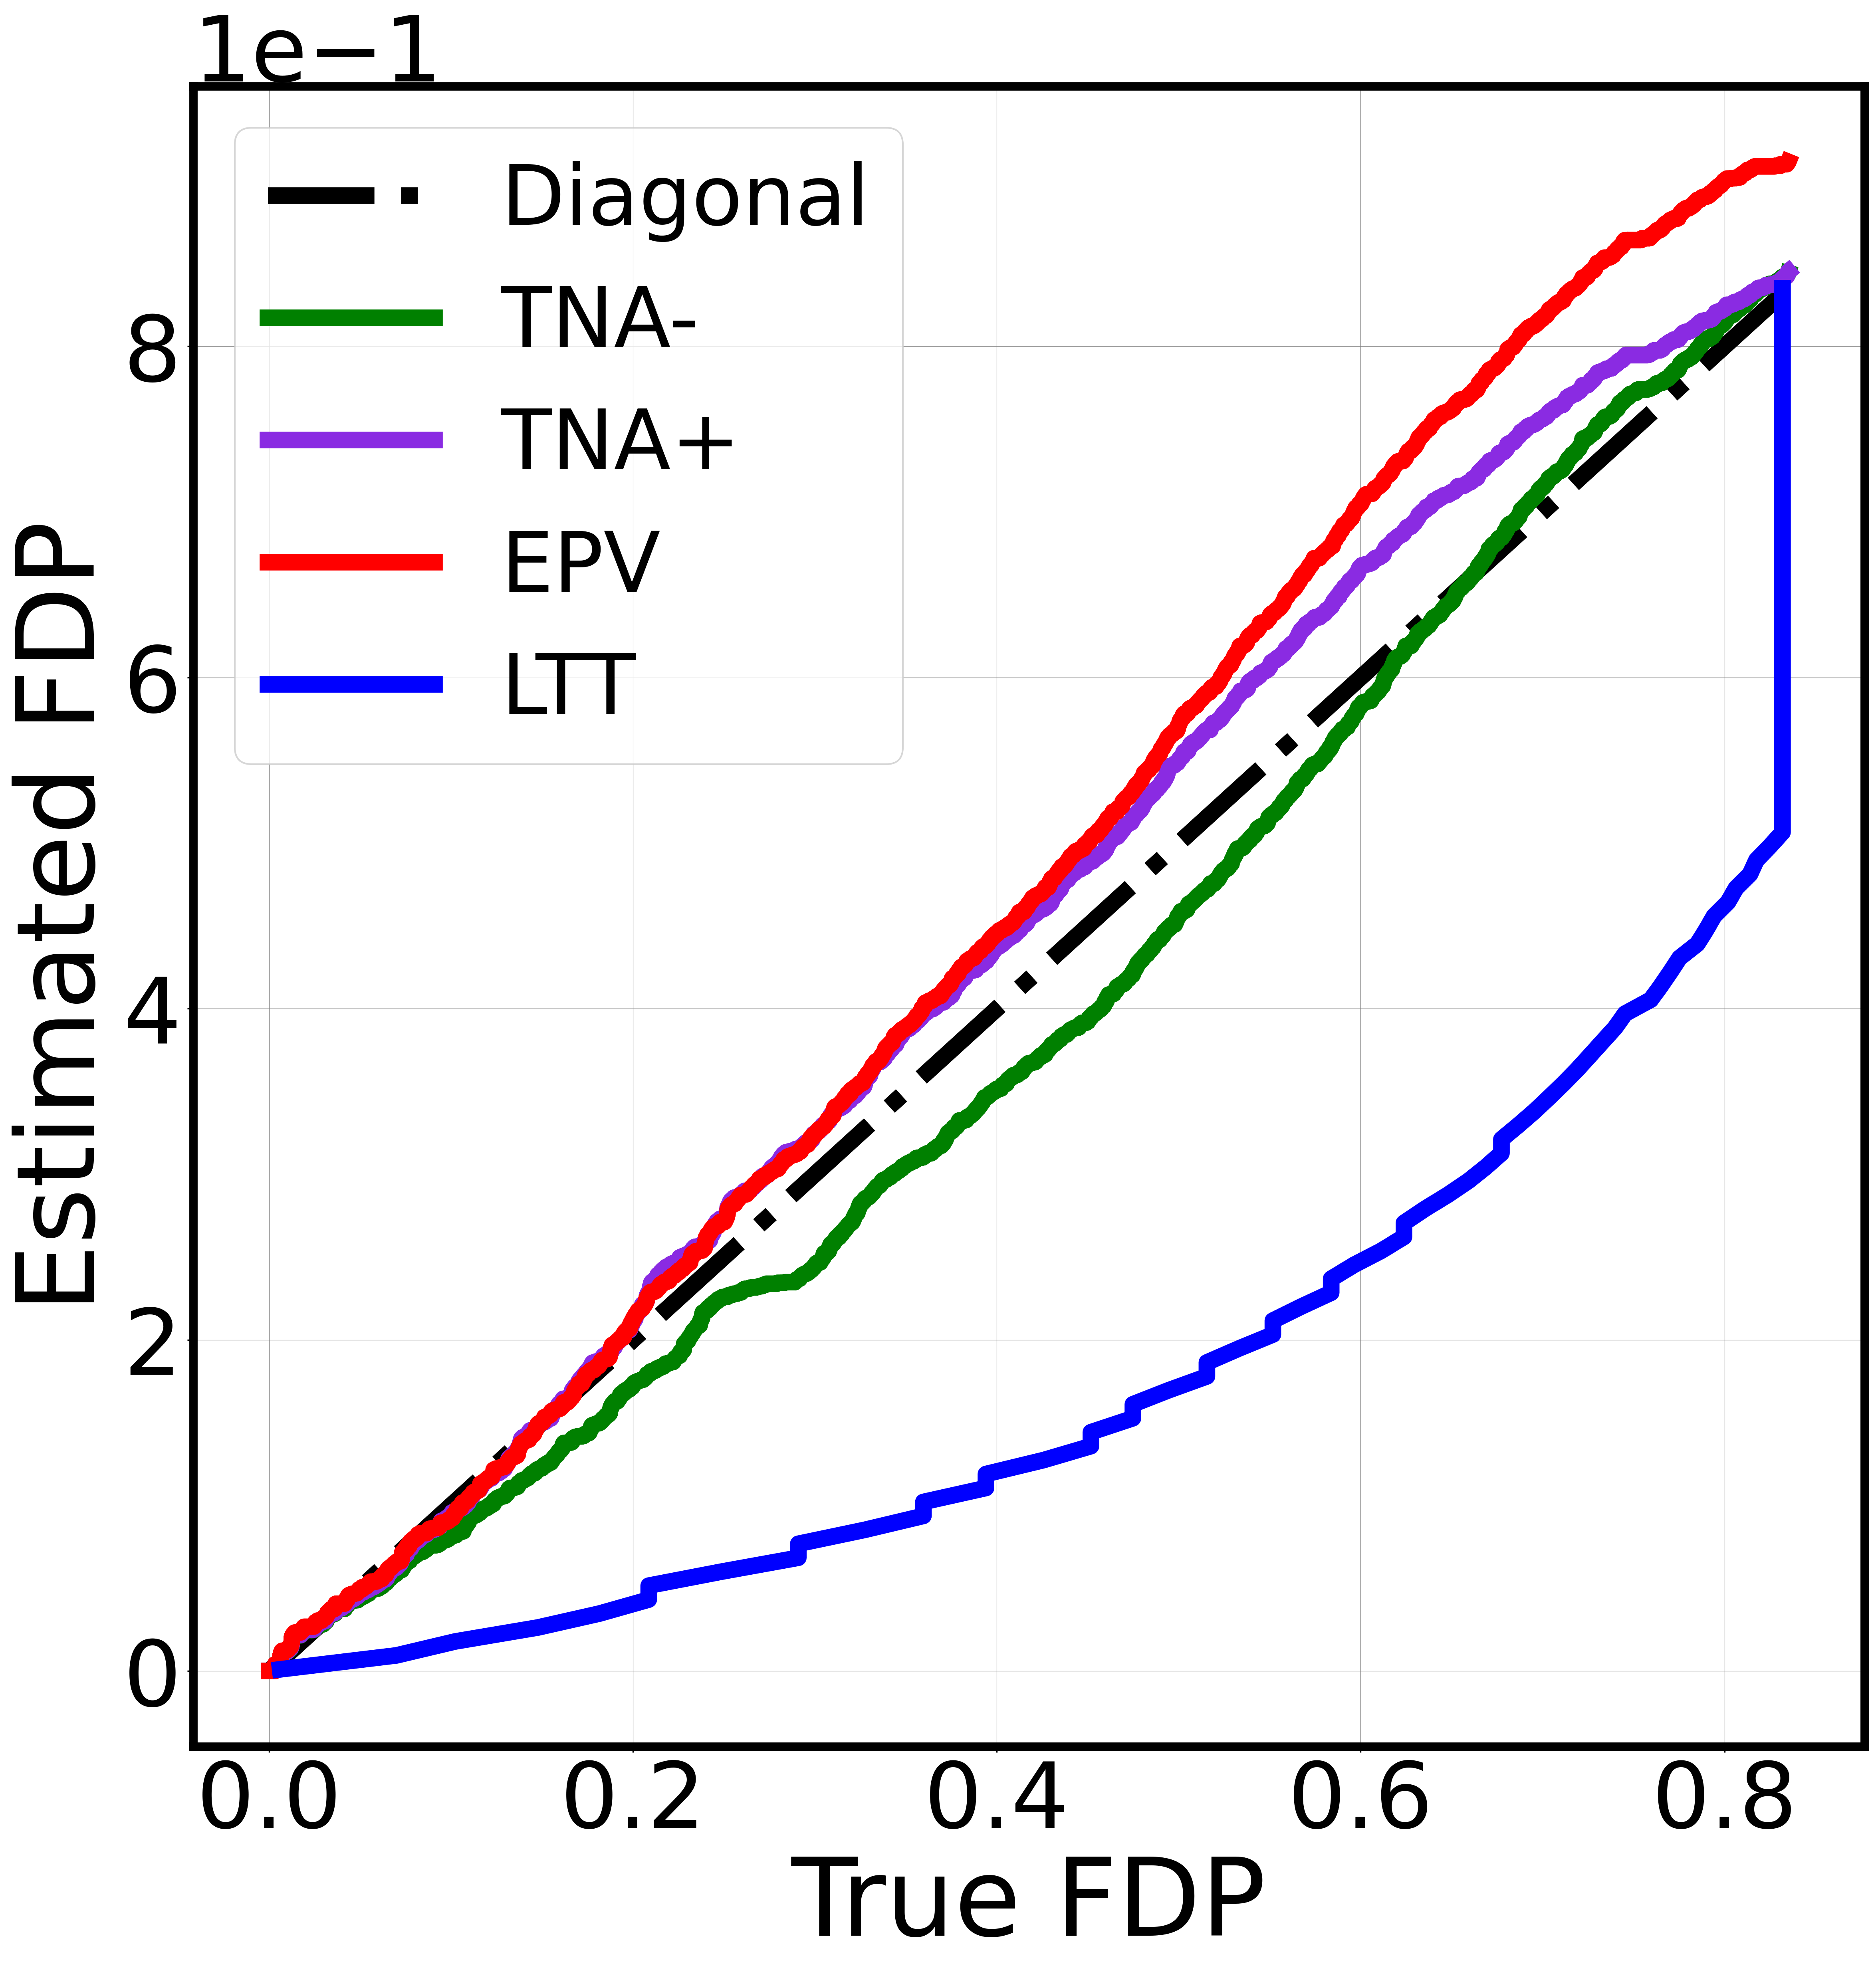
\includegraphics[width=1.7in]{img/cnn_FDPscat_pcam_balanced.png}
%		\\	
%		A & B & C & D
%	\end{tabular}
%	\caption{{\bf FDR control on PCam dataset under class distribution shift.} (A) QQ plot of the EPVs (red dots) and the TNA EPVs (green dots) against the theoretical uniform distribution. The results of the Fisher's combination tests are indicated in the legend. The EPVs are slight inflated,  (B) The number of accepted classifications as a function of the Q-values obtained with (i) ground truth (black line), (ii) BH with EPV (red), (iii) BH with TNA EPV (green), and (iv) LTT (blue). (C) Same as (B) but over a critical Q-value range. (D) Deviation of the estimated FDR from the actual FDR obtained with (i) BH with EPV (red line), (ii) BH with EPV and TNA (green line), (iii) LTT (blue line).}
%	\label{fig:pcam_rebalance}
%\end{figure} 

\subsection{TissueNet: cells segmentation}

\begin{figure}
    \centering
	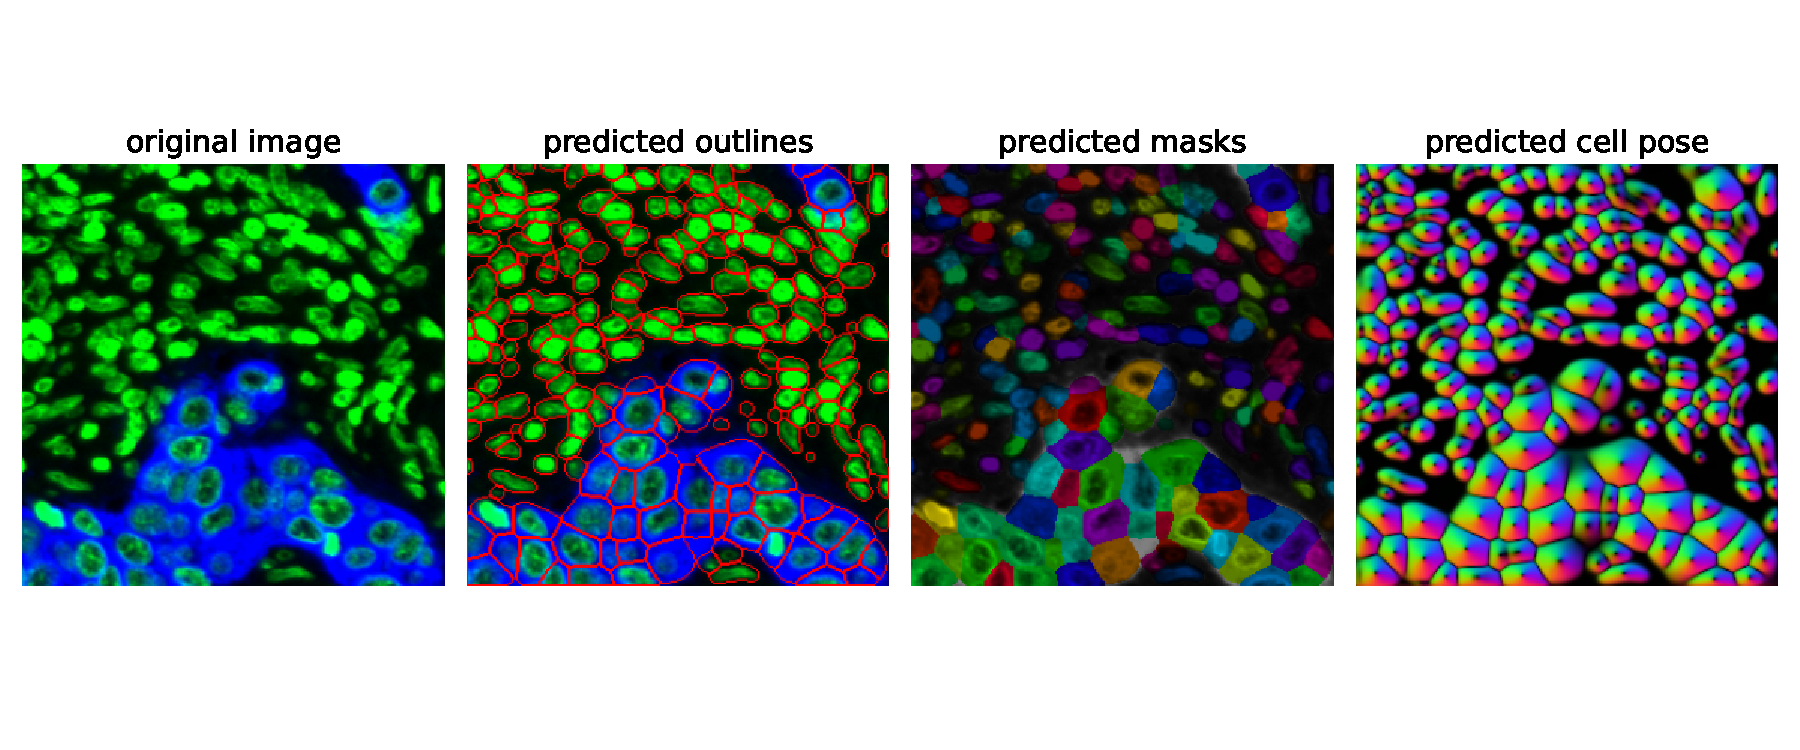
\includegraphics[width=5in]{img/tissuenet.pdf}
	\caption{{\bf Instance of TissueNet dataset.} Two-channel original images are being processed by the model, in turn producing masks \& flows to correctly segment cells}
	\label{fig:tissue_example}
\end{figure} 

TissueNet dataset contains 1.3 million microscopic images of cells obtained from six various platforms and nine organs including both histologically healthy and diseased tissues. Each images has a size of 512x512 pixels. Each image was manually segmented at pixel level and paired whole-cell and nuclear annotations. Our binary classification task was to predict whether a pixel is inside a cell (positive) or not (negative). The overall positive:negative ration was 59:41\% in the training data and 66:34\% in the test data; however, the class ratio varies over the images considerably. We used the Cellpose pre-trained deep neural network model \cite{cellpose}, we fine tuned it for five epochs, and it achieves 95\% and 94\% of accuracies  on training and test data, respectively. Our evaluation is reported on Figure \ref{fig:pcam}-(iii). The plots reveal that the BH protocol with standard EPVs becomes liberally biased; i.e. the actual FDR is higher than the true FDR. This can be seen in the Figure  \ref{fig:pcam}-(iii)-D. As a consequence, it yields more trusted predictions at any q-value levels than the ground truth, c.f. dashed-red and black solid lines on Figure \ref{fig:pcam}-(iii)-BC. This bias might originate from data distribution shift, possibly resulting from overfitting. Both, LTT and the BH with TNA EPV remain accurate in the critical region (0-15 \% FDRs); however, both methods become conservative  at loos FDR levels (>15 \%). Conservative estimation is preffered in practice to liberal one; hoever, in this case we think this was just a mere coincidence. 

However, when we run the tests on a single images, 
%
%\begin{figure}
%	\centering
%	\begin{tabular}{cccc}
%		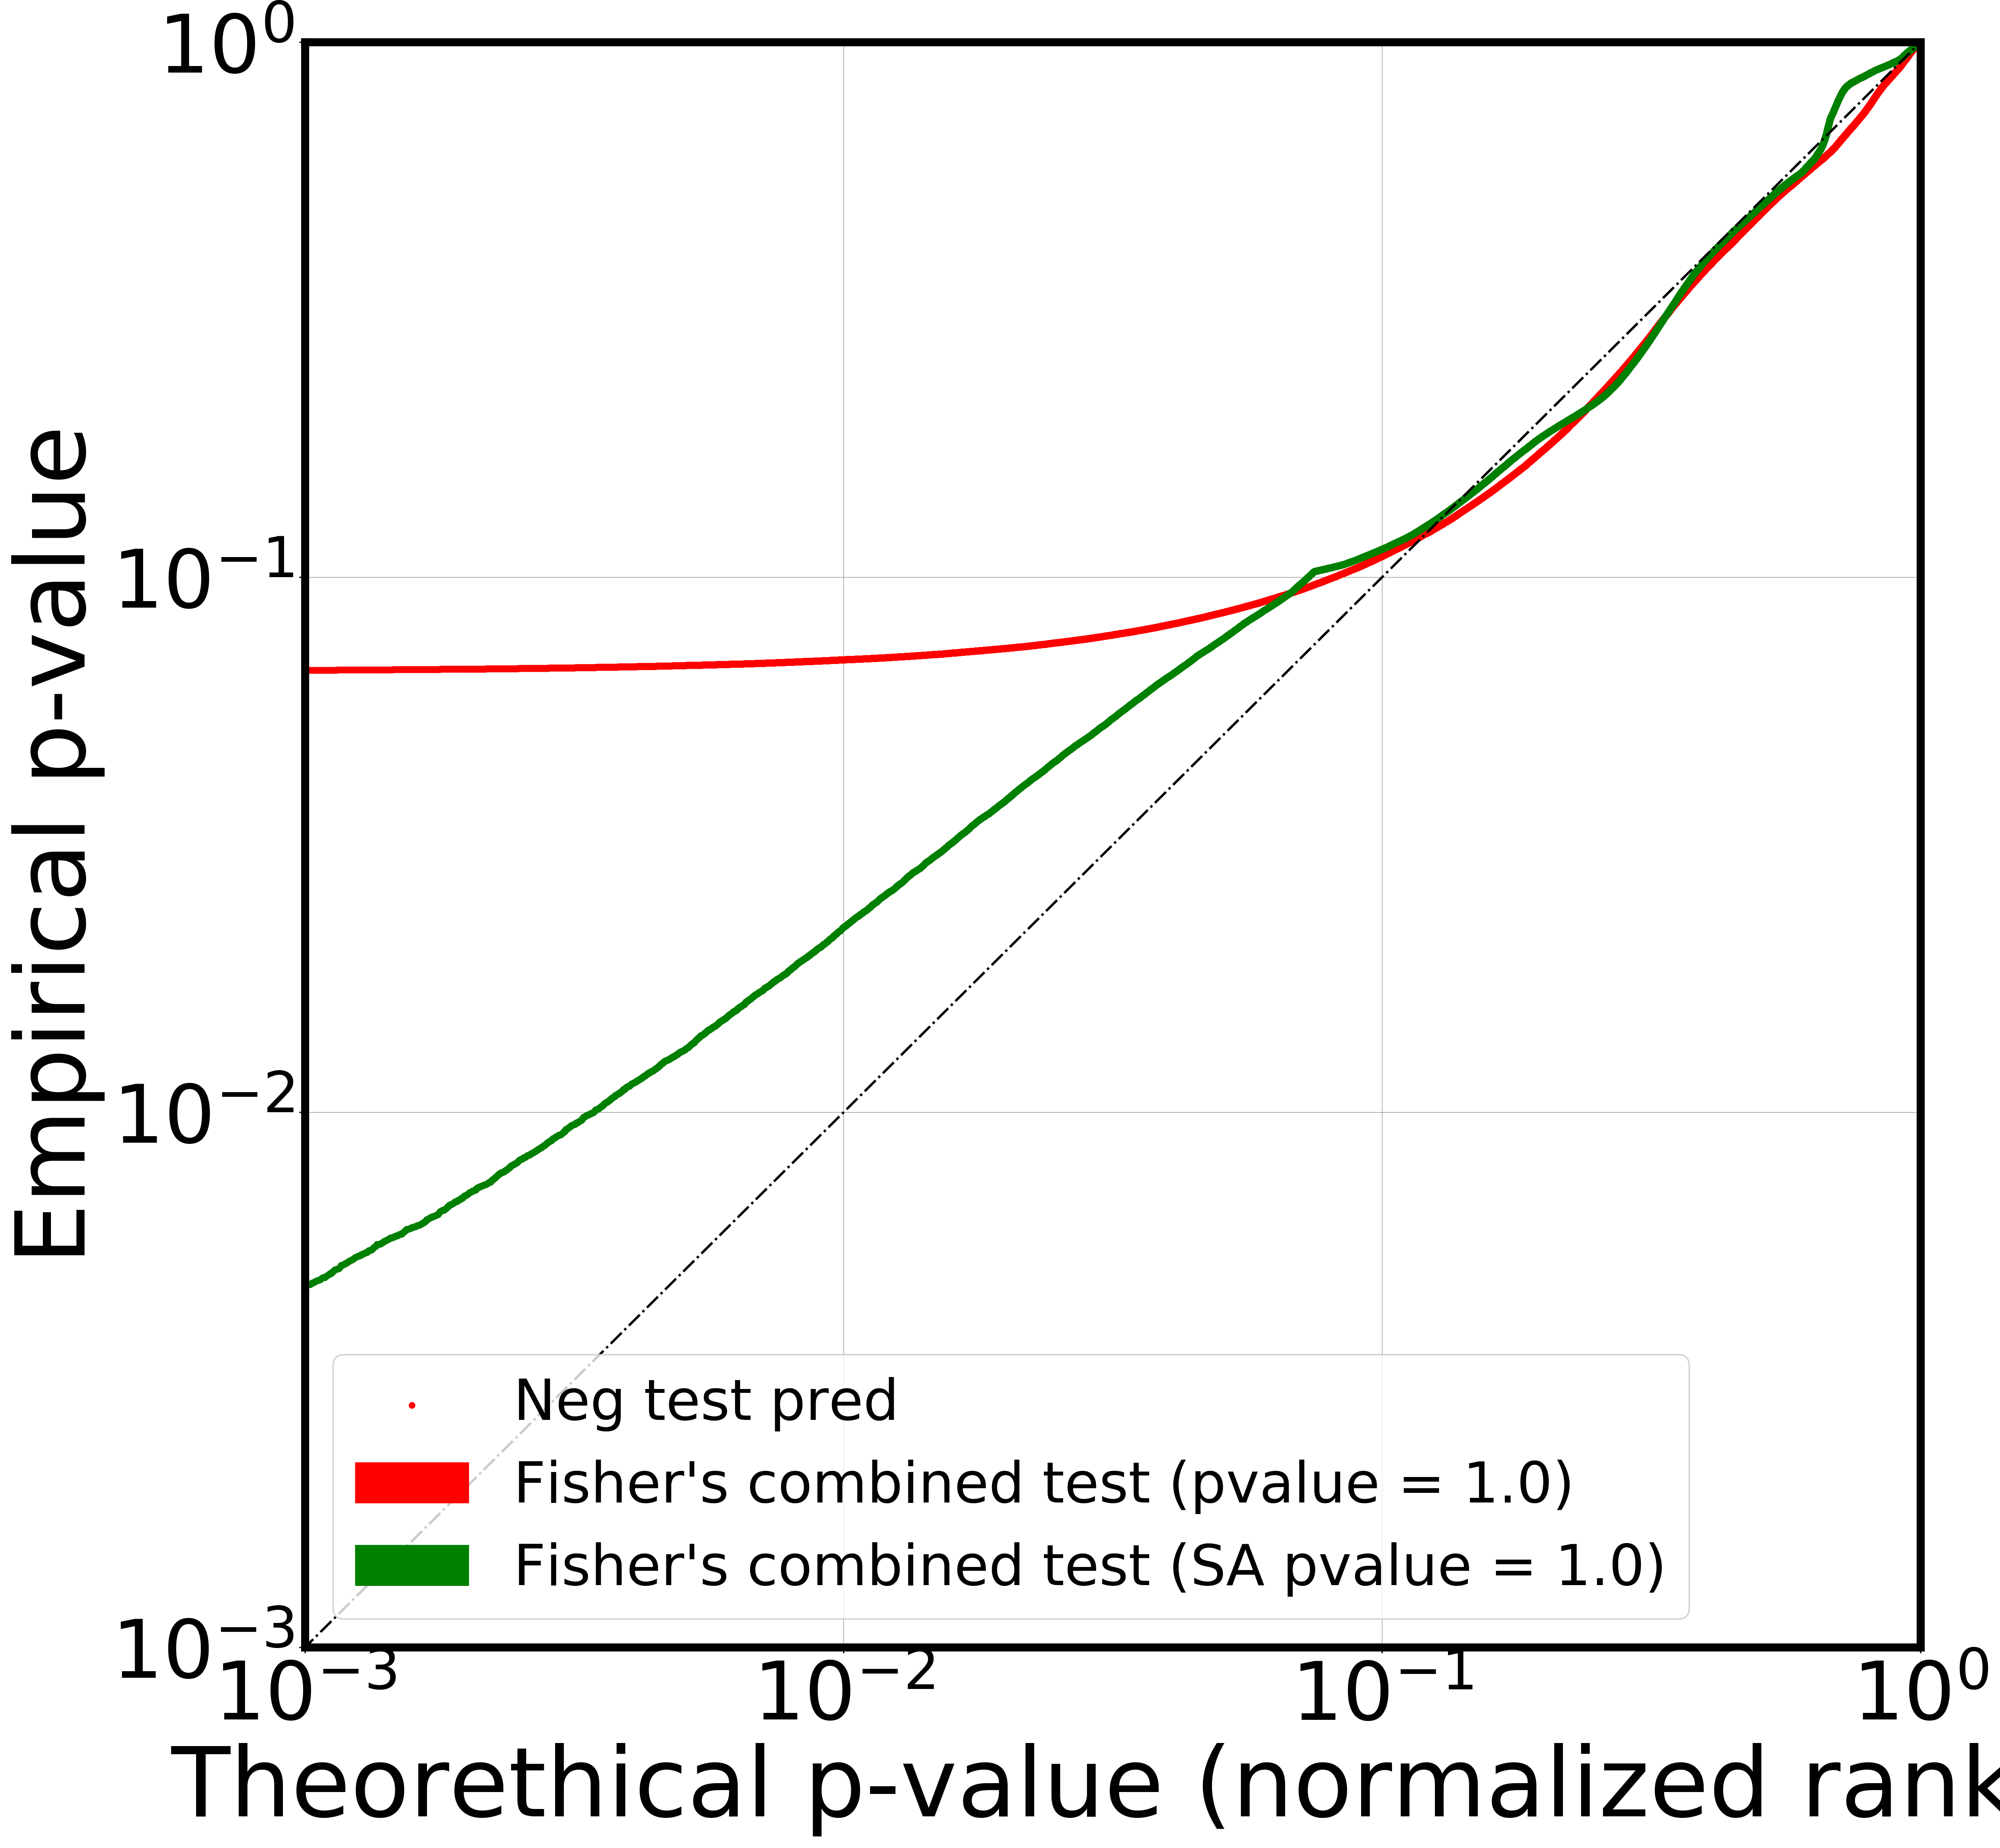
\includegraphics[width=1.7in]{img/cnn_QQ_cells_segment_TA_log.png} &
%		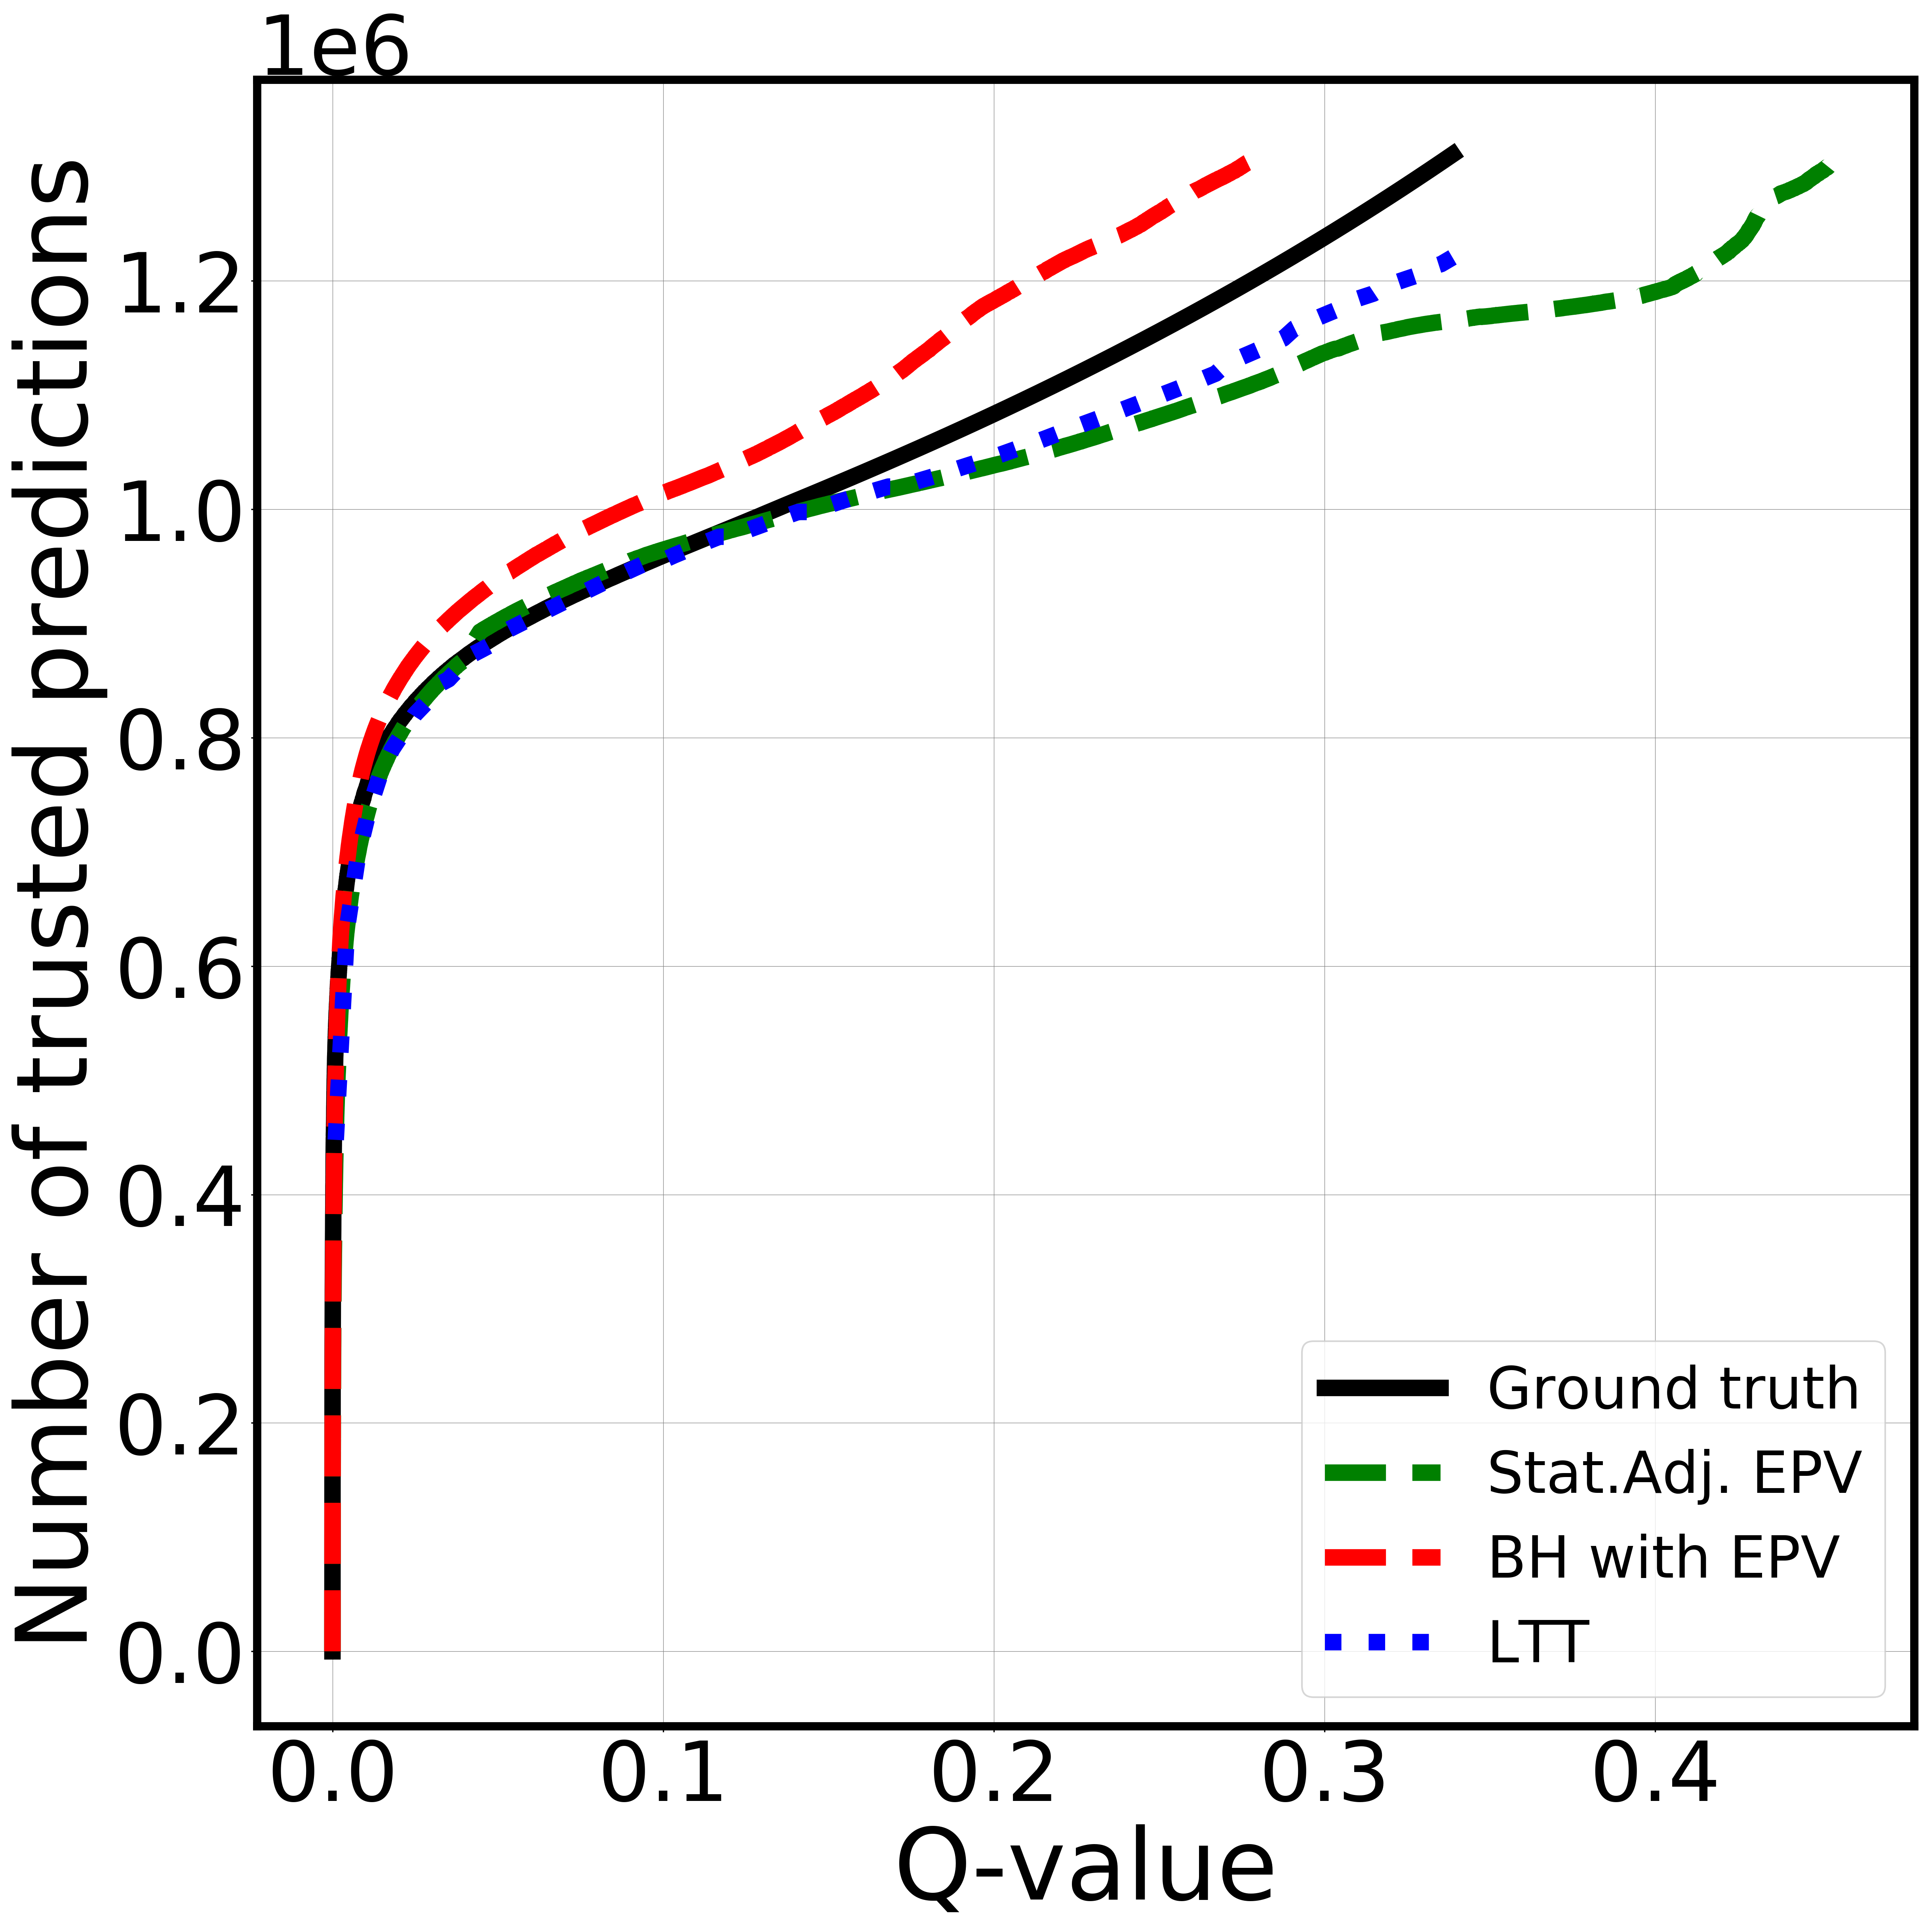
\includegraphics[width=1.7in]{img/cnn_cells_segment_TA_fdr_control.png} & 
%        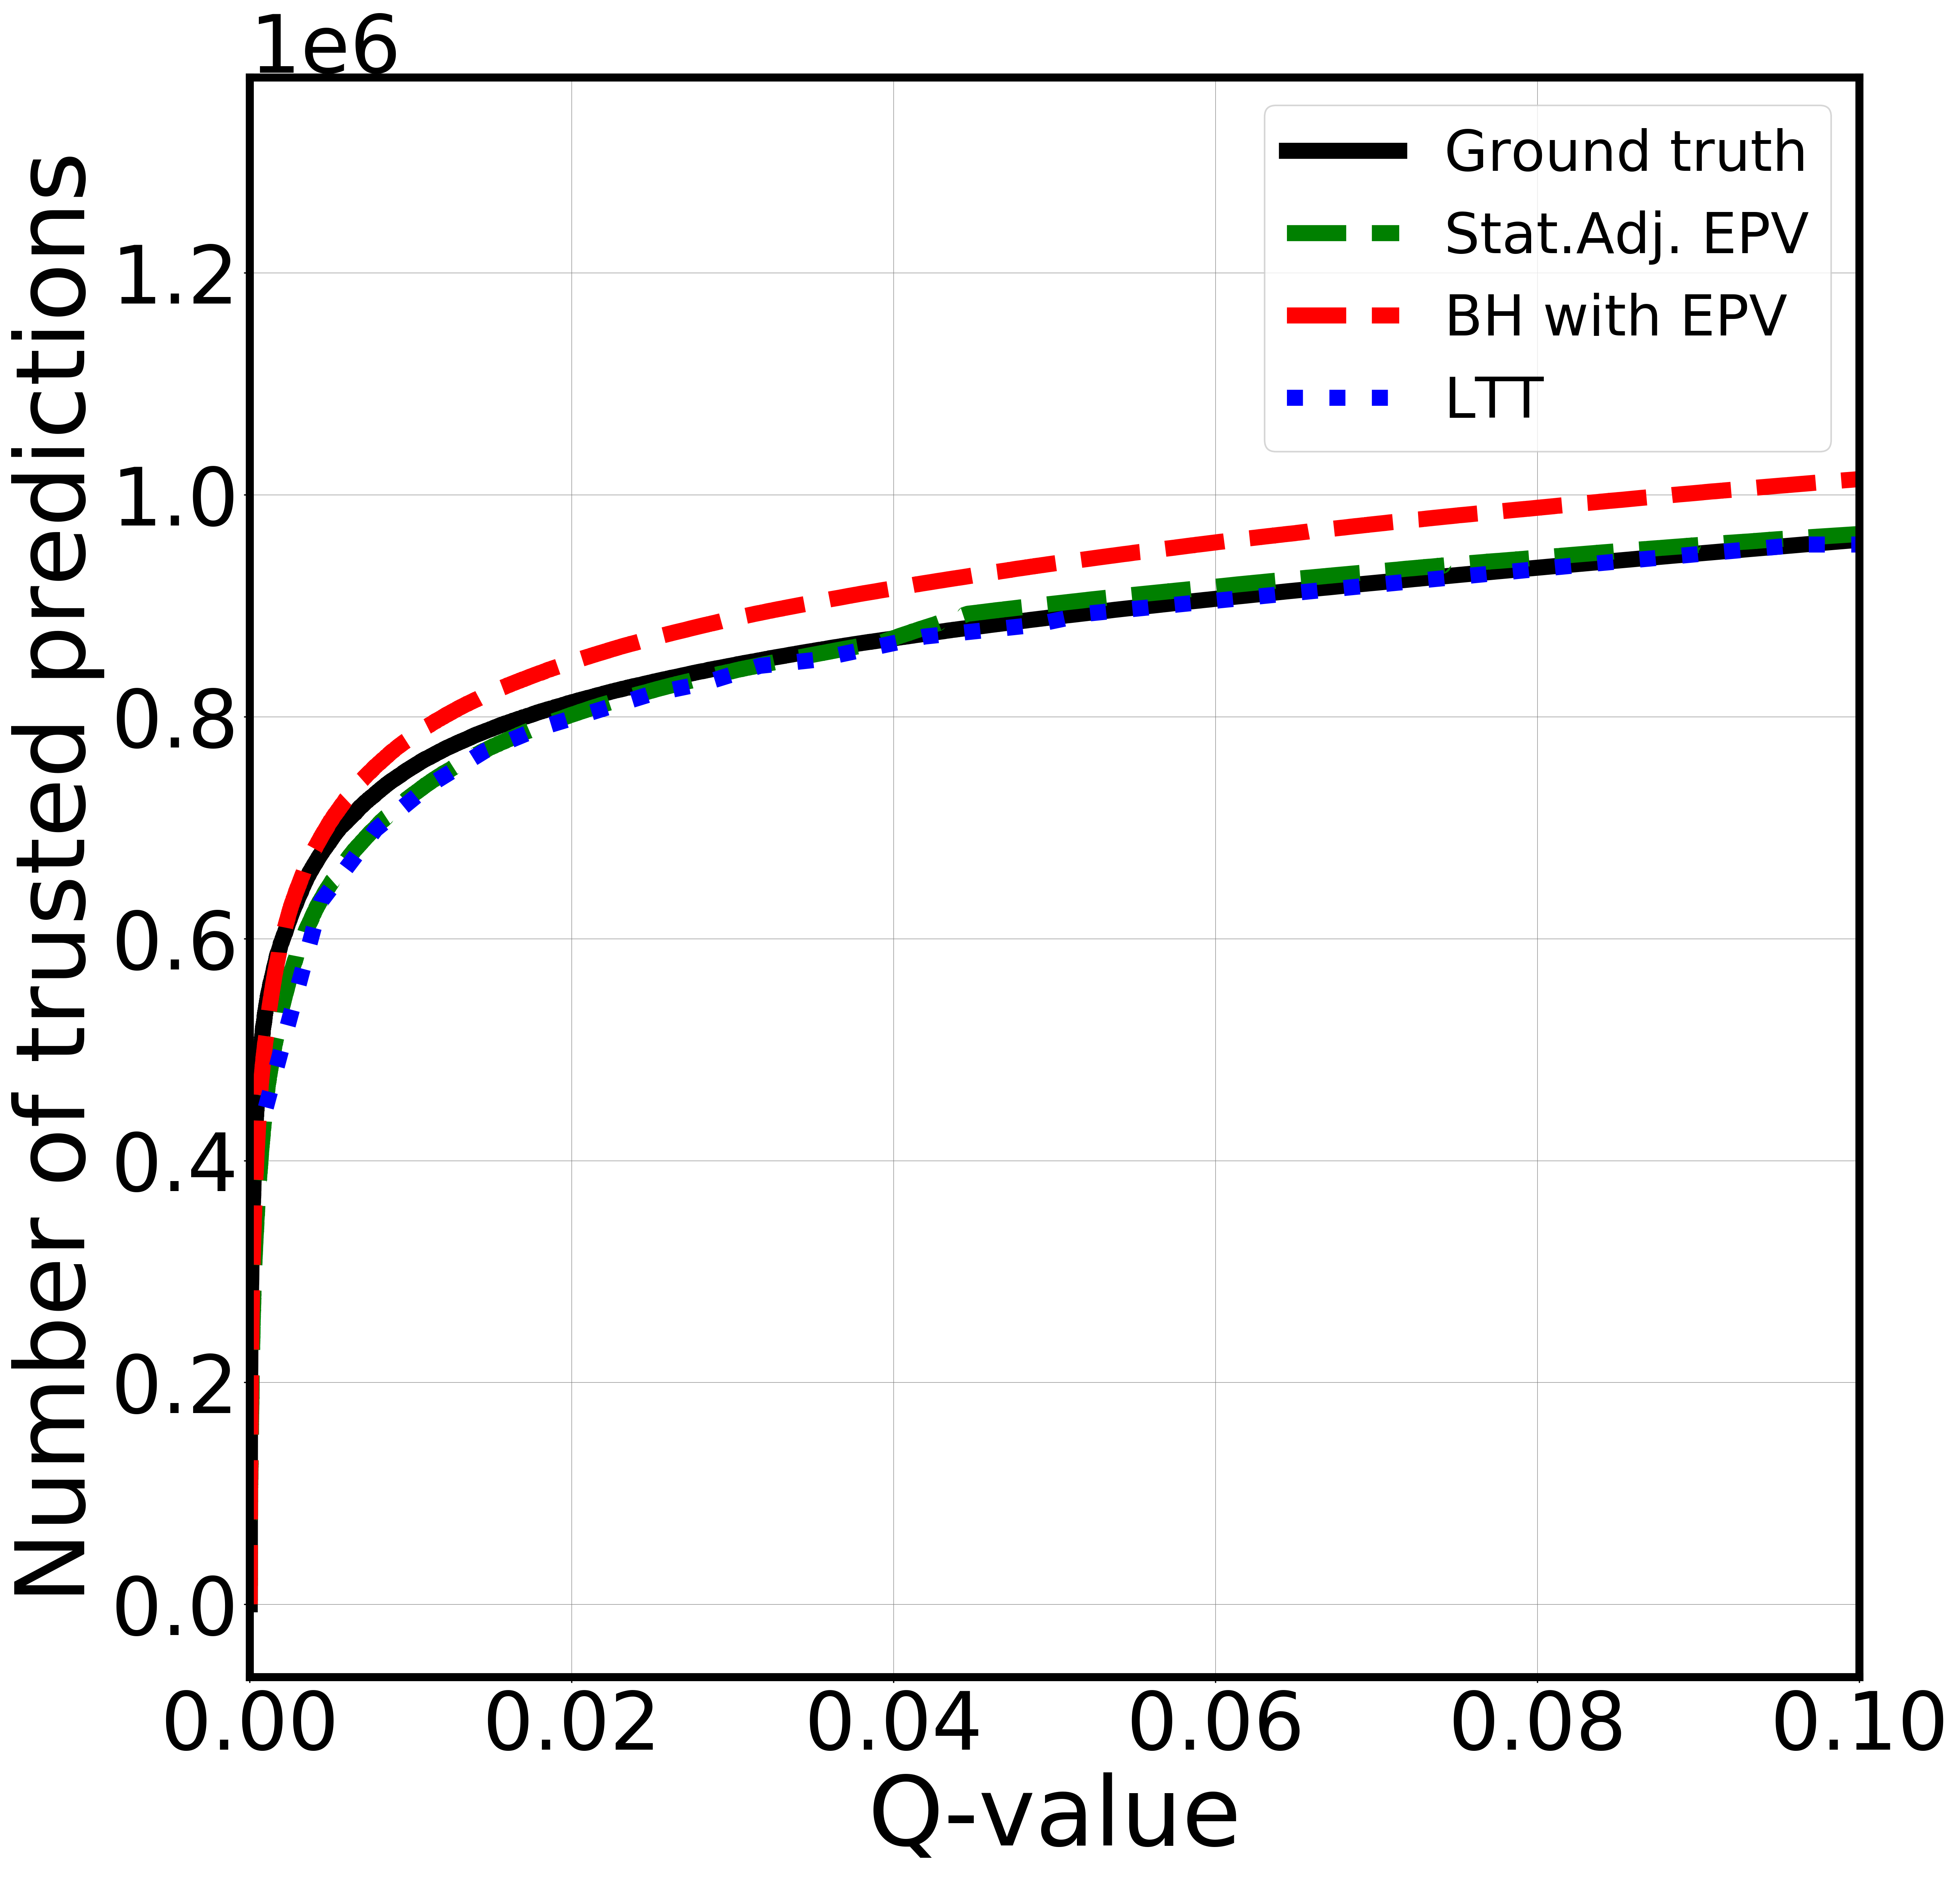
\includegraphics[width=1.7in]{img/cnn_cells_segment_TA_fdr_control_loc.png} & 
%            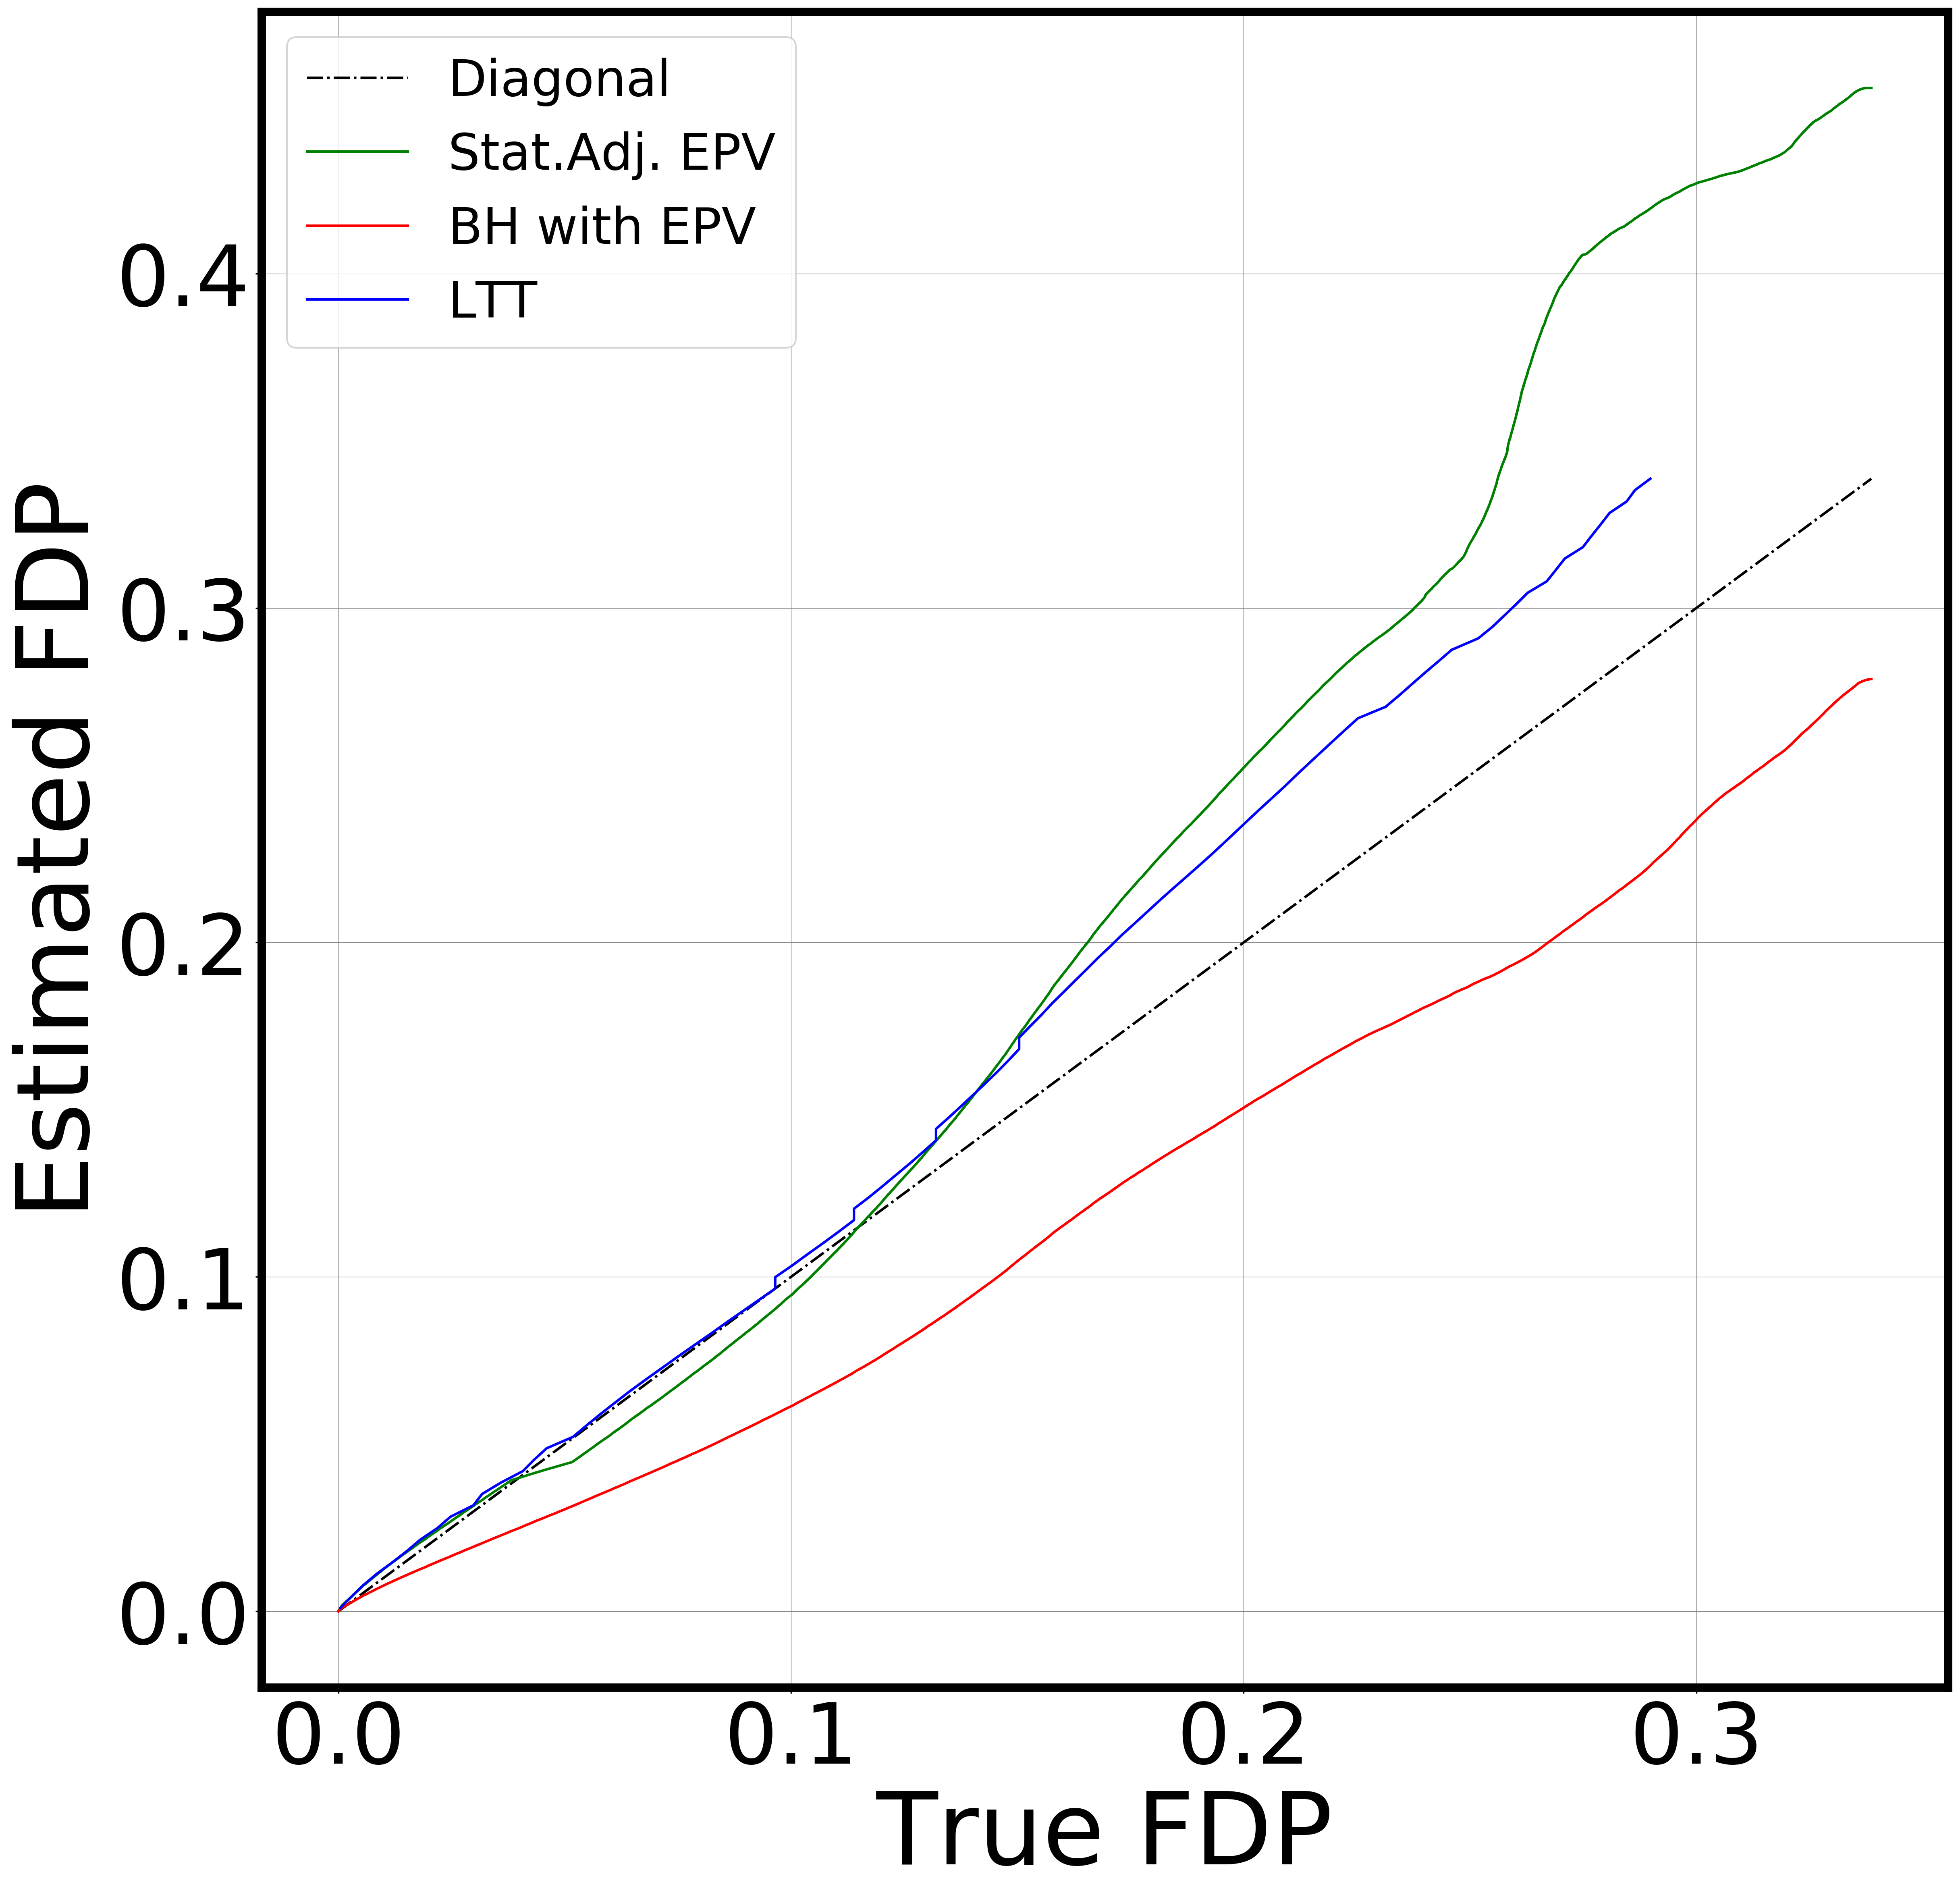
\includegraphics[width=1.7in]{img/cnn_FDPscat_cells_segment_TA.png}\\	
%		A & B & C & D
%	\end{tabular}
%	\caption{\bf FDR control with p-values for TissueNet dataset.}
%	\label{fig:tissue}
%\end{figure}
%

%
%\begin{figure}
%	\centering
%	\begin{tabular}{cccc}
% 		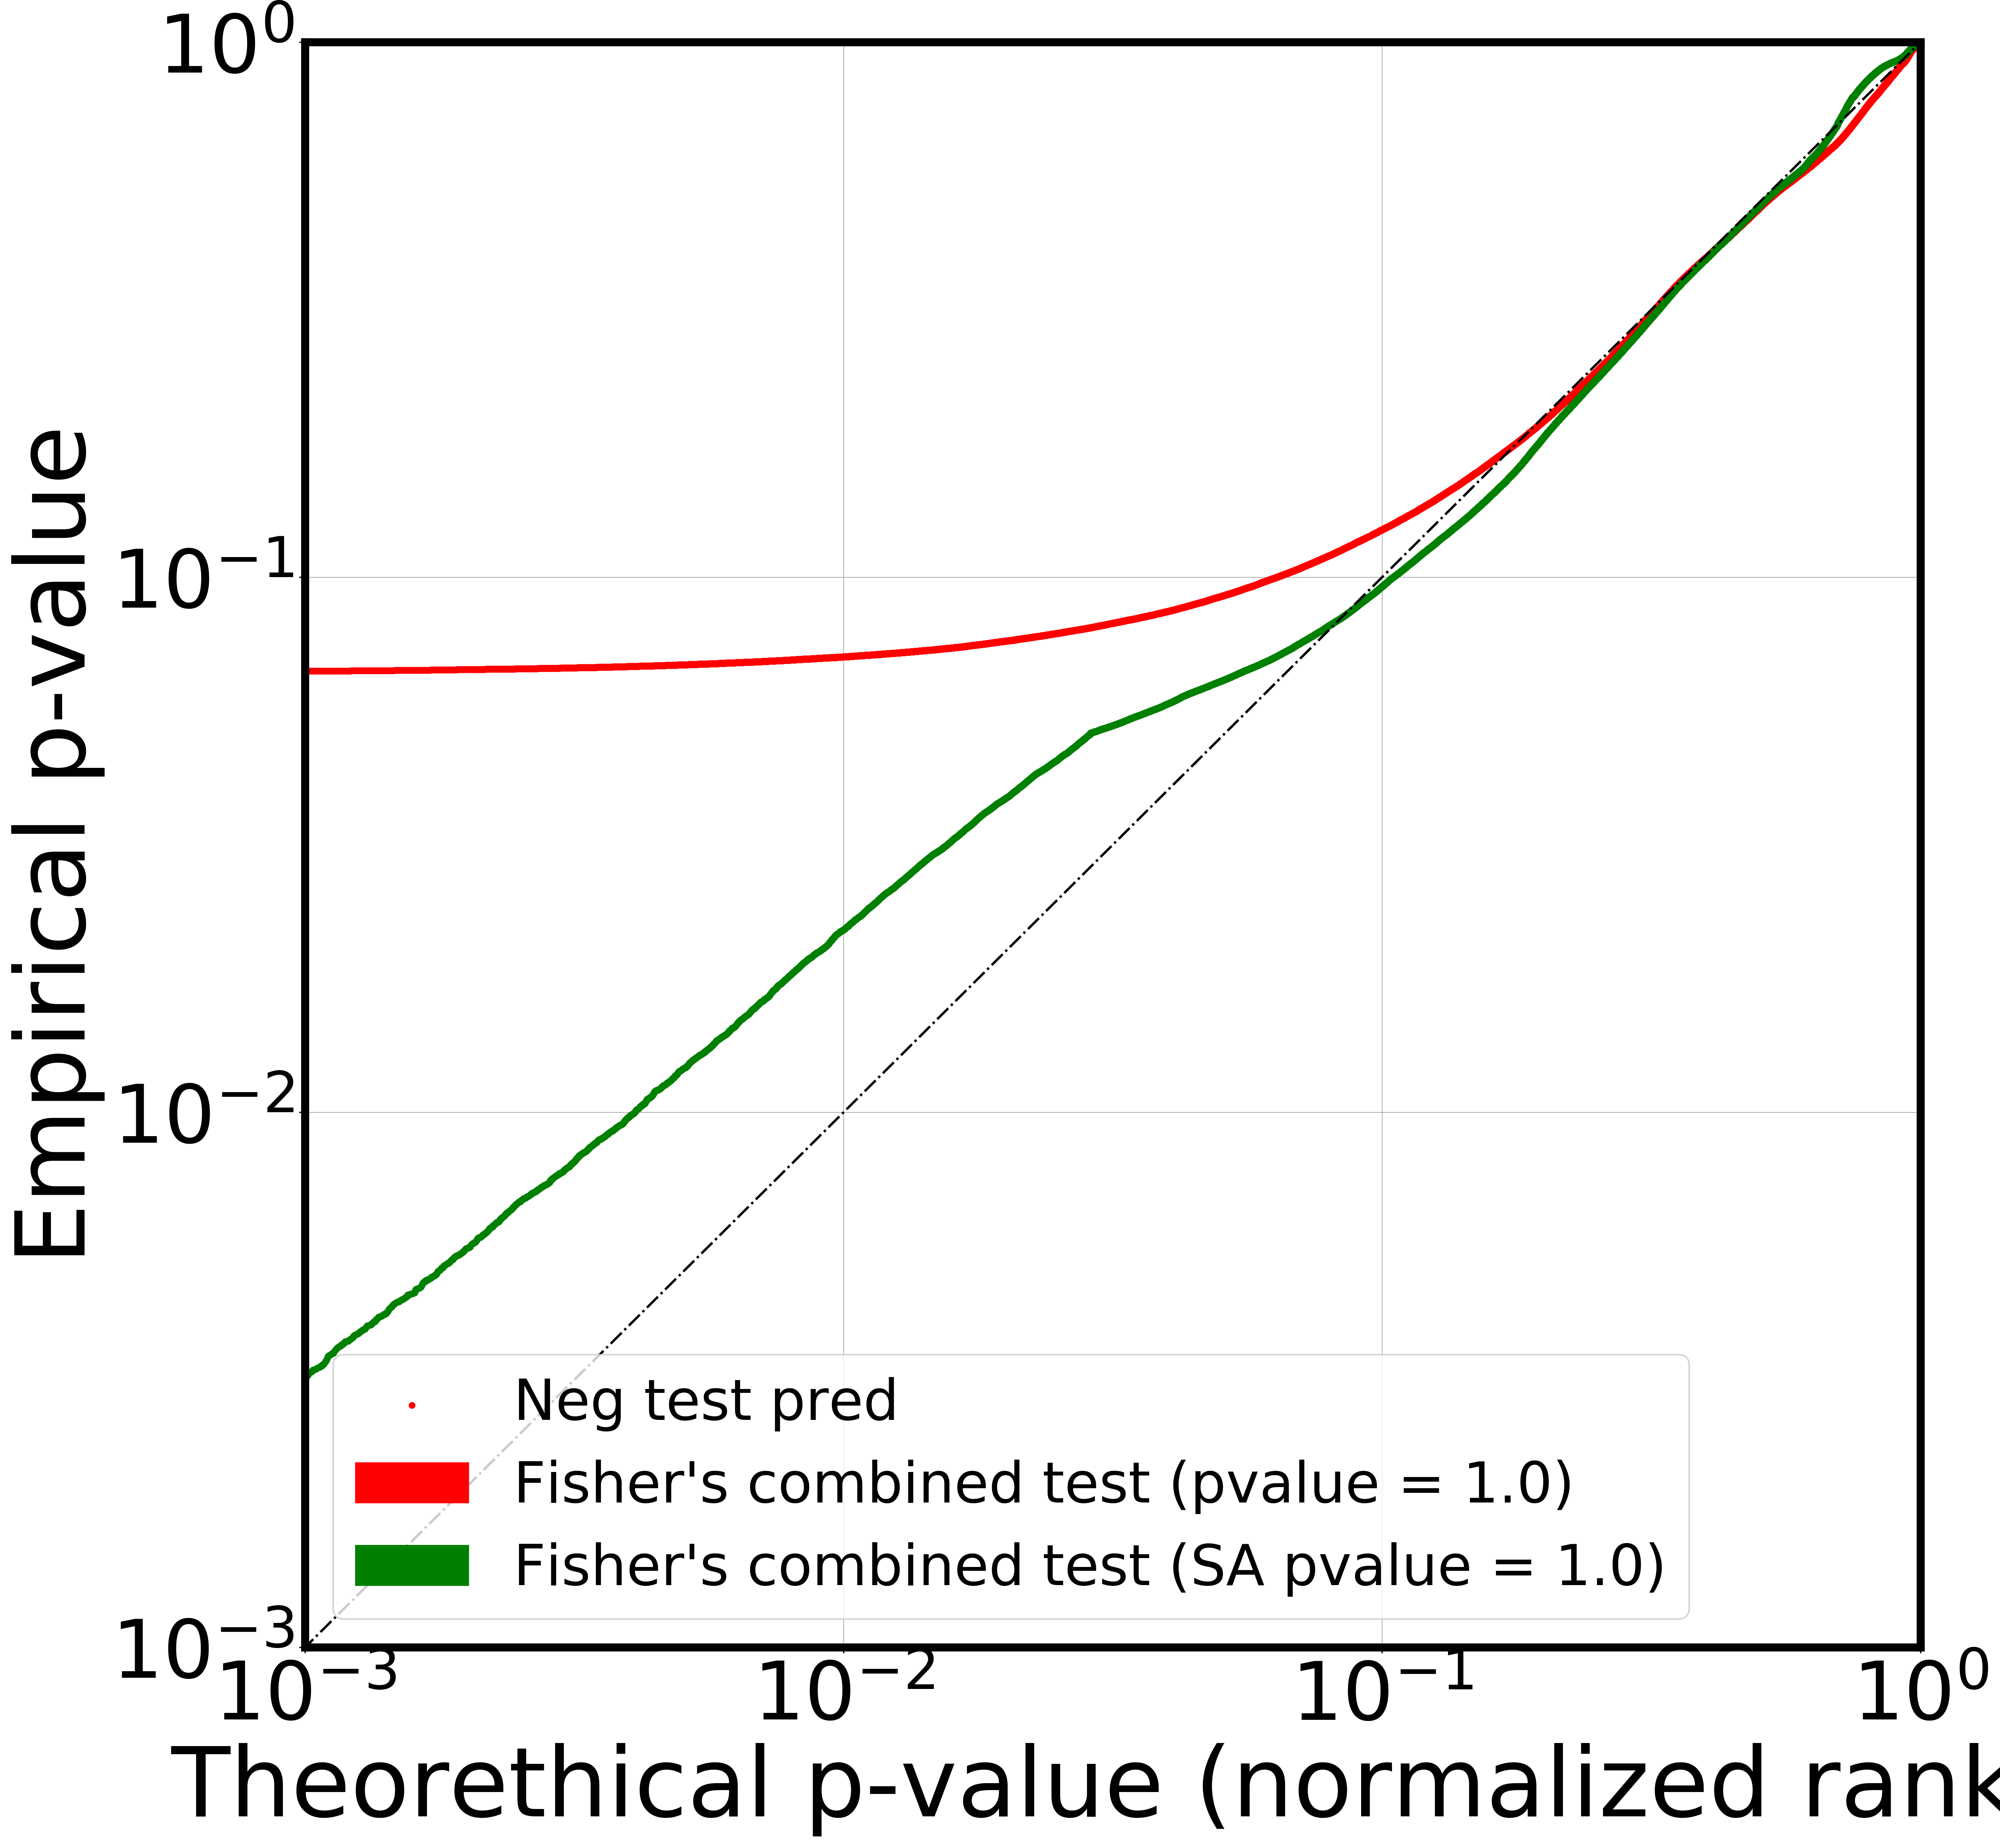
\includegraphics[width=1.7in]{img/cnn_QQ_cells_balanced_TA_log.png} &
%		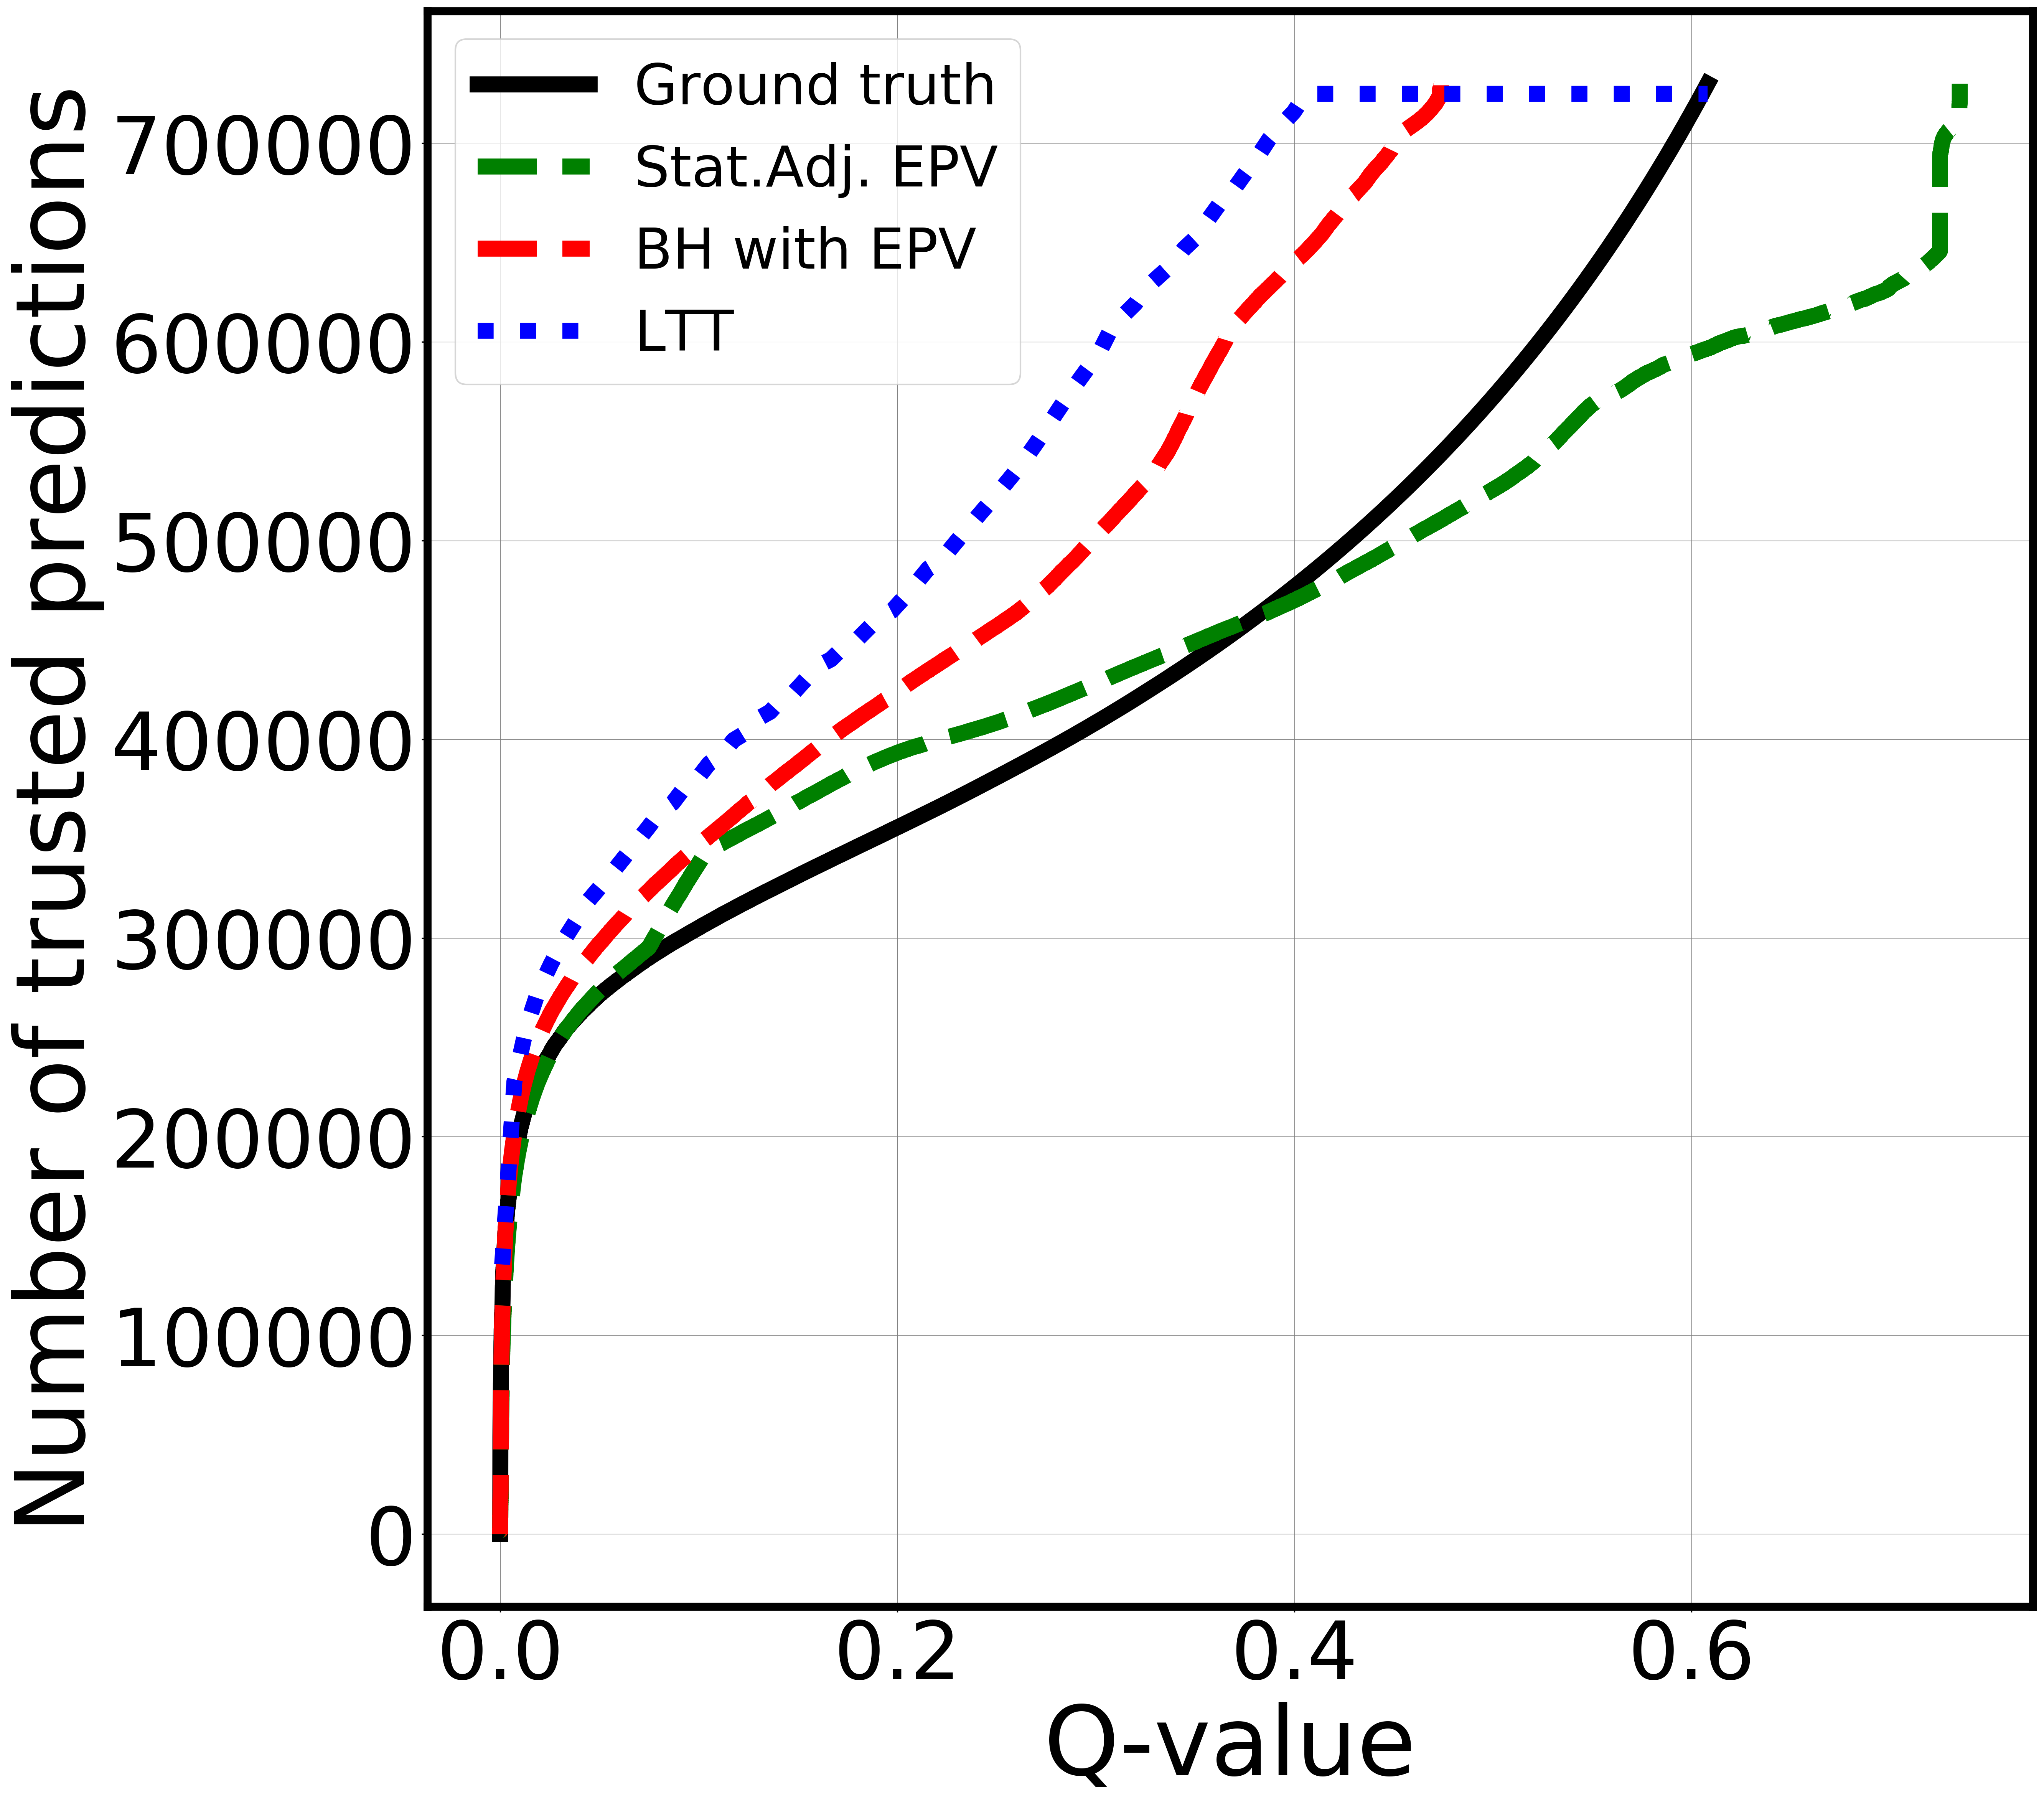
\includegraphics[width=1.7in]{img/cnn_cells_balanced_TA_fdr_control.png} & 
%            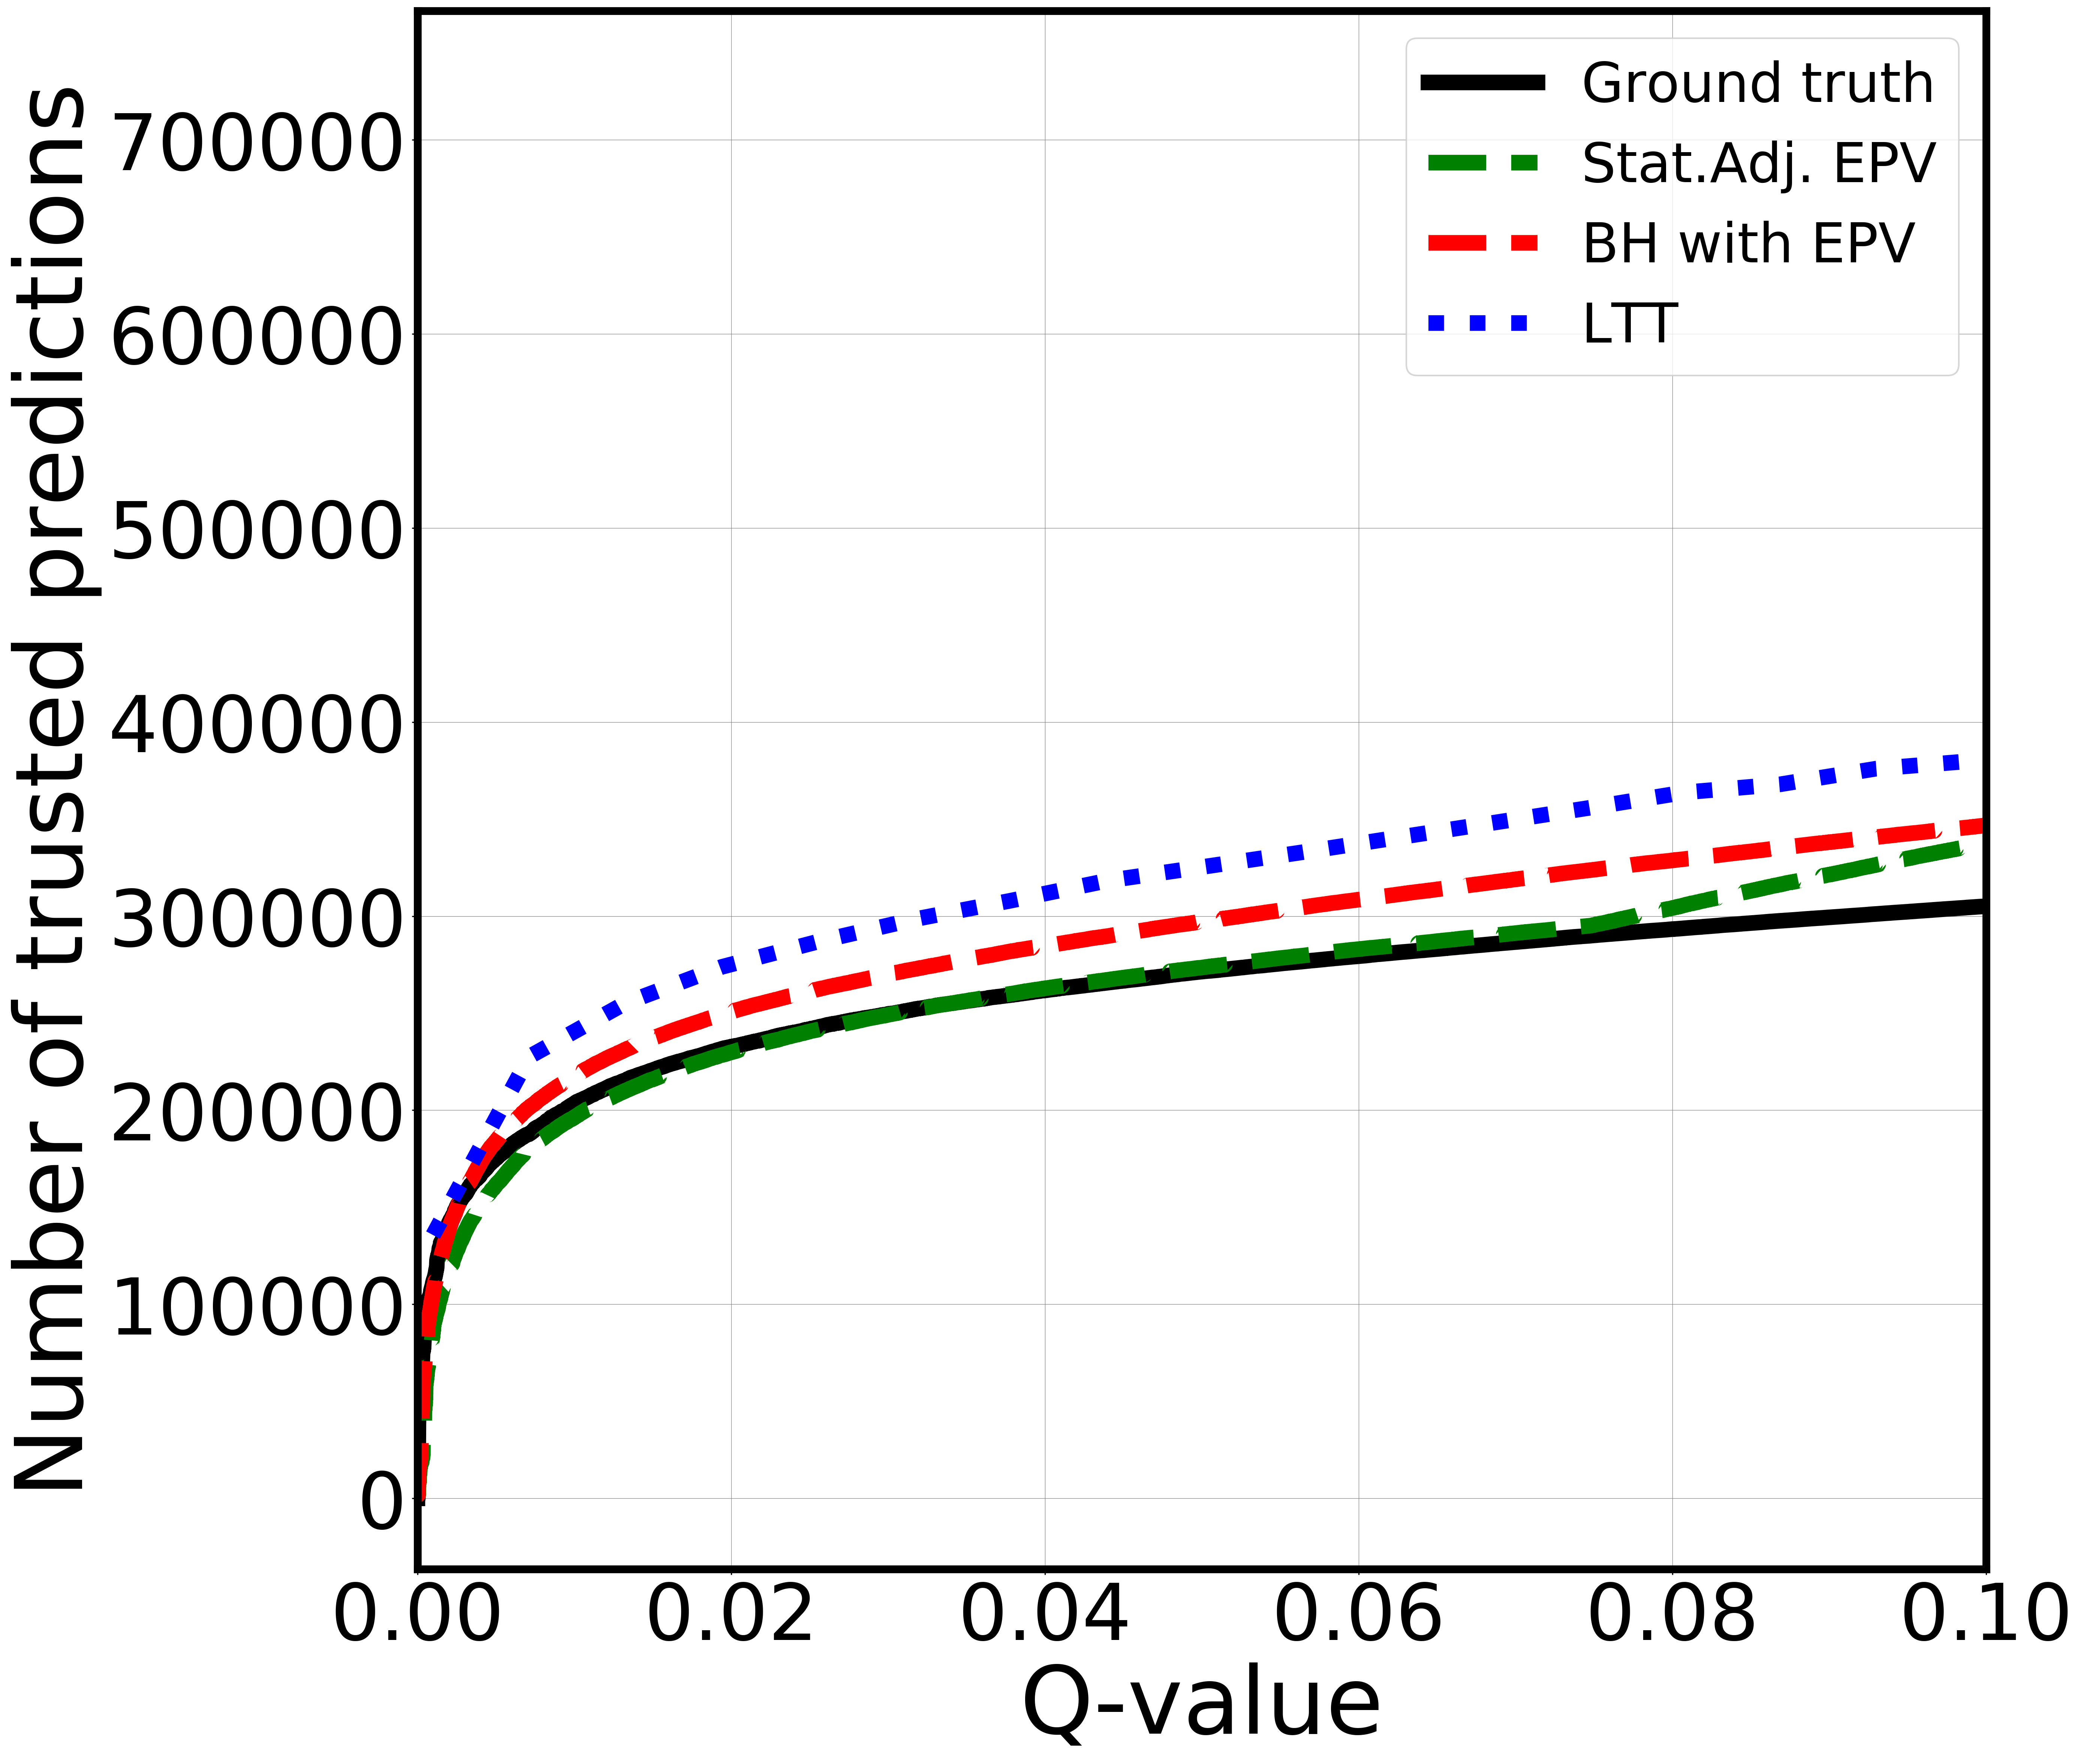
\includegraphics[width=1.7in]{img/cnn_cells_balanced_TA_fdr_control_loc.png} & 
%            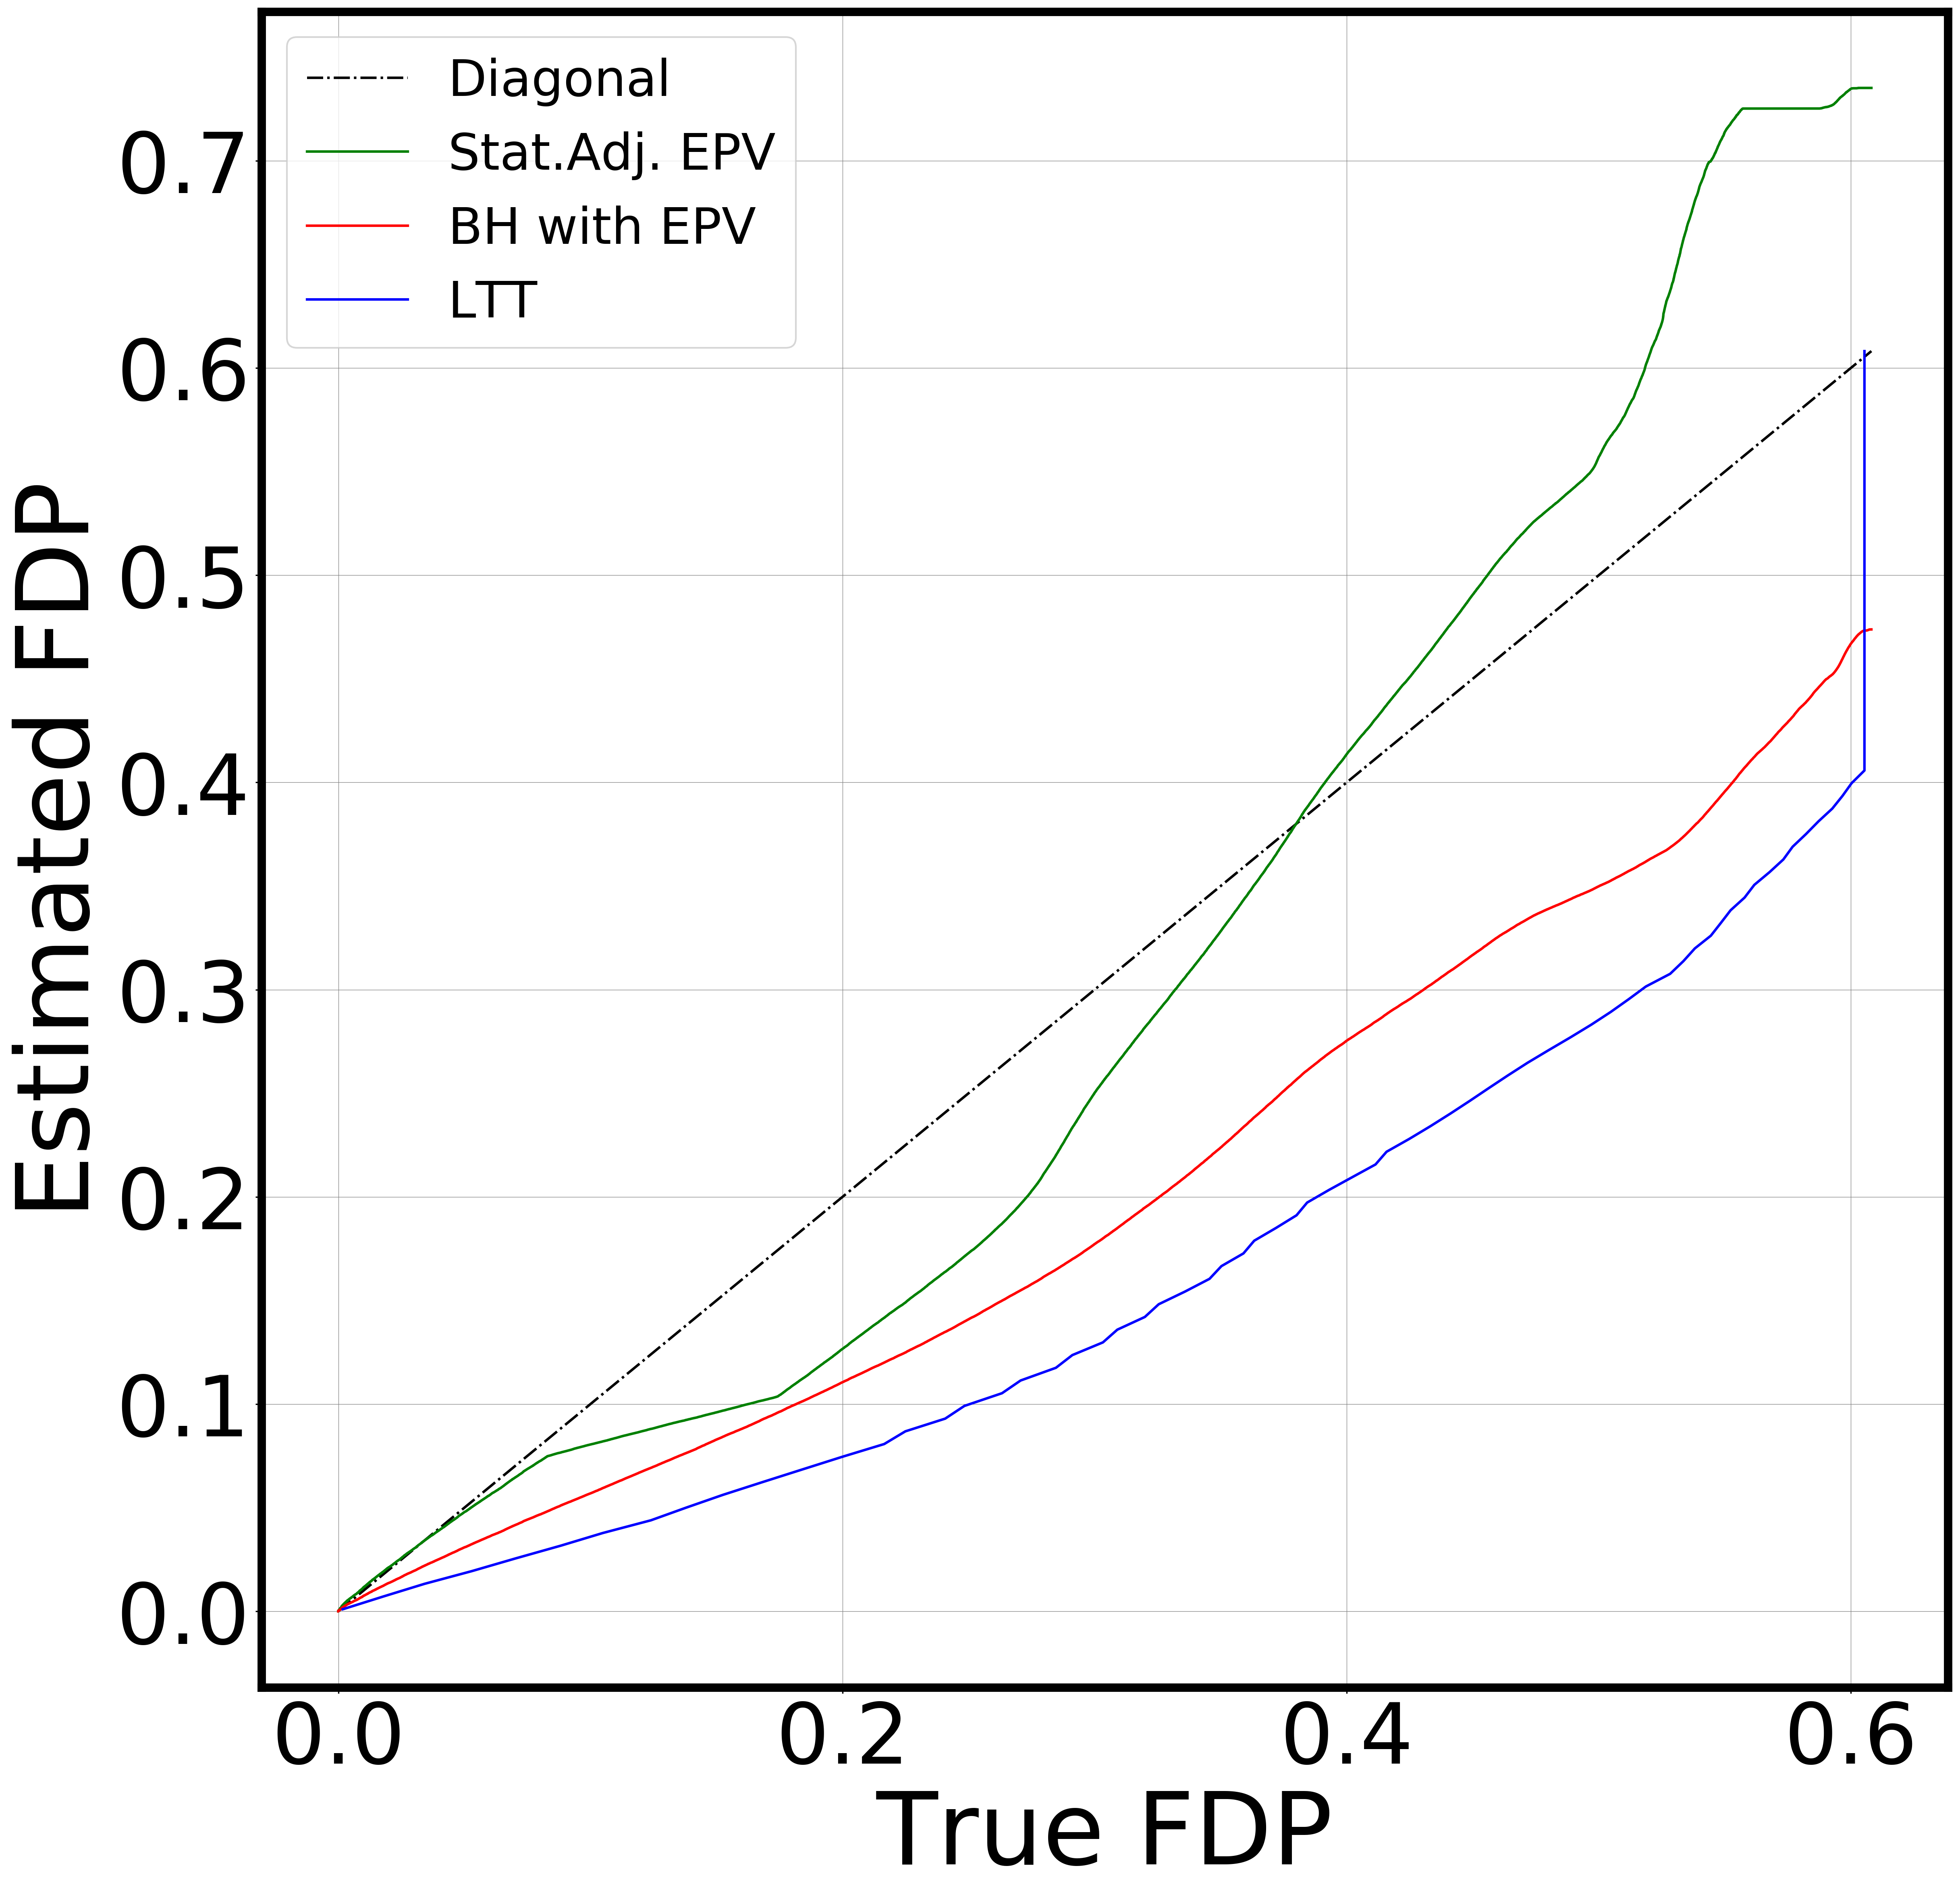
\includegraphics[width=1.7in]{img/cnn_FDPscat_cells_balanced_TA.png}\\	
%		A & B & C & D
%	\end{tabular}
%	\caption{\bf FDR control with p-values for rebalanced TissueNet dataset.}
%	\label{fig:tissue_rebalance}
%\end{figure}



\subsection{BCSS: Breast cancer semantic segmentation dataset}

\begin{figure}[h]
	\centering
	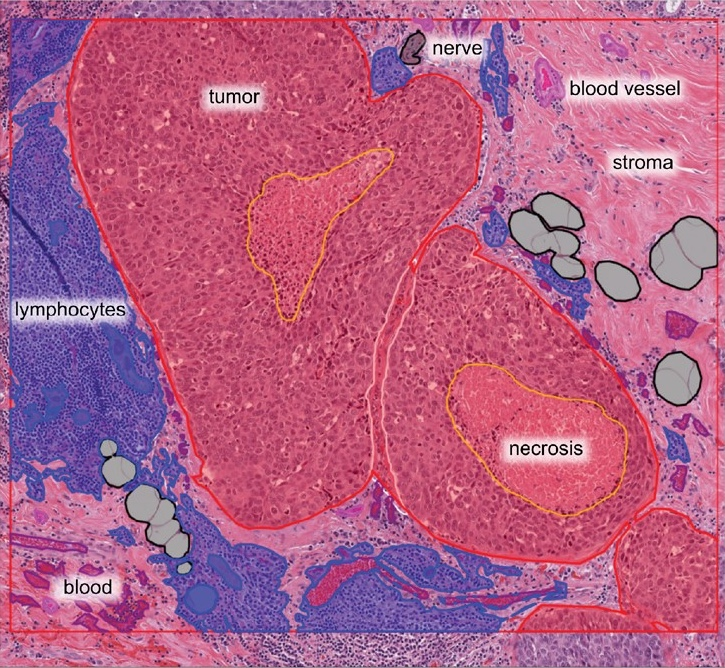
\includegraphics[width=3in]{img/bcss_instance.jpeg}
	\caption{{\bf An instance from BCSS dataset.}}
	\label{fig:bcss_example}
\end{figure} 

The Breast Cancer Semantic Segmentation (BCSS) dataset \cite{Amgad2019StructuredCE} contains around 20,000 image segmentation images annotated with Digital Slide Archive, with a particular focus on tissue regions derived from breast cancer imagery obtained from The Cancer Genome Atlas (TCGA). The image pixels are labeled by: 'Stroma', 'Tumor' and 'Others', and the corresponding class ratios in both the training and test sets are: 54\% : 38\% : 8\%. We used the deep learning model called \texttt{'fcn resnet50 unet-bcss'} from the TIA (Tissue Image Analysis) toolbox \cite{Pocock2022} to classify the pixels to one of the four classes. The model achieved an 84 \% and 82 \% accuracies on the training and test datasets. 

We note that, because this dataset involves multi-class classification, we slightly modified the FDR control procedure. We calculated the p-values, the $\pi_0$ estimations and then the corresponding q-values with BH procedure with respect to single classes; then we associated the minimal q-value and its class label  to each test instance. Therefore, an trusted prediction means that a sample is correctly classified.

Our FDR evaluation is presented in Figure \ref{fig:bcss}-(i). We note that, we did not evaluate LTT here, because it is not clear how to adjust it to multi-class classification problems. The results reveal that BH with standard EPVs becomes overly liberal, possibly to data shift, while BH with TNA EPVs remains somewhat close to the ground truth. We also note that the ``flat step'' at the beginning of the ground truth indicates that the model's most confident predictions are incorrect. 

However, when we run the tests on a single images,  the standard BH becomes even worse or better. \todo{AB}{come on!} 



\begin{figure}[h!]
	
	\begin{tabular}{cccc}
		\multicolumn{4}{l}{\bf (i) Standard PCam dataset:}\\		
		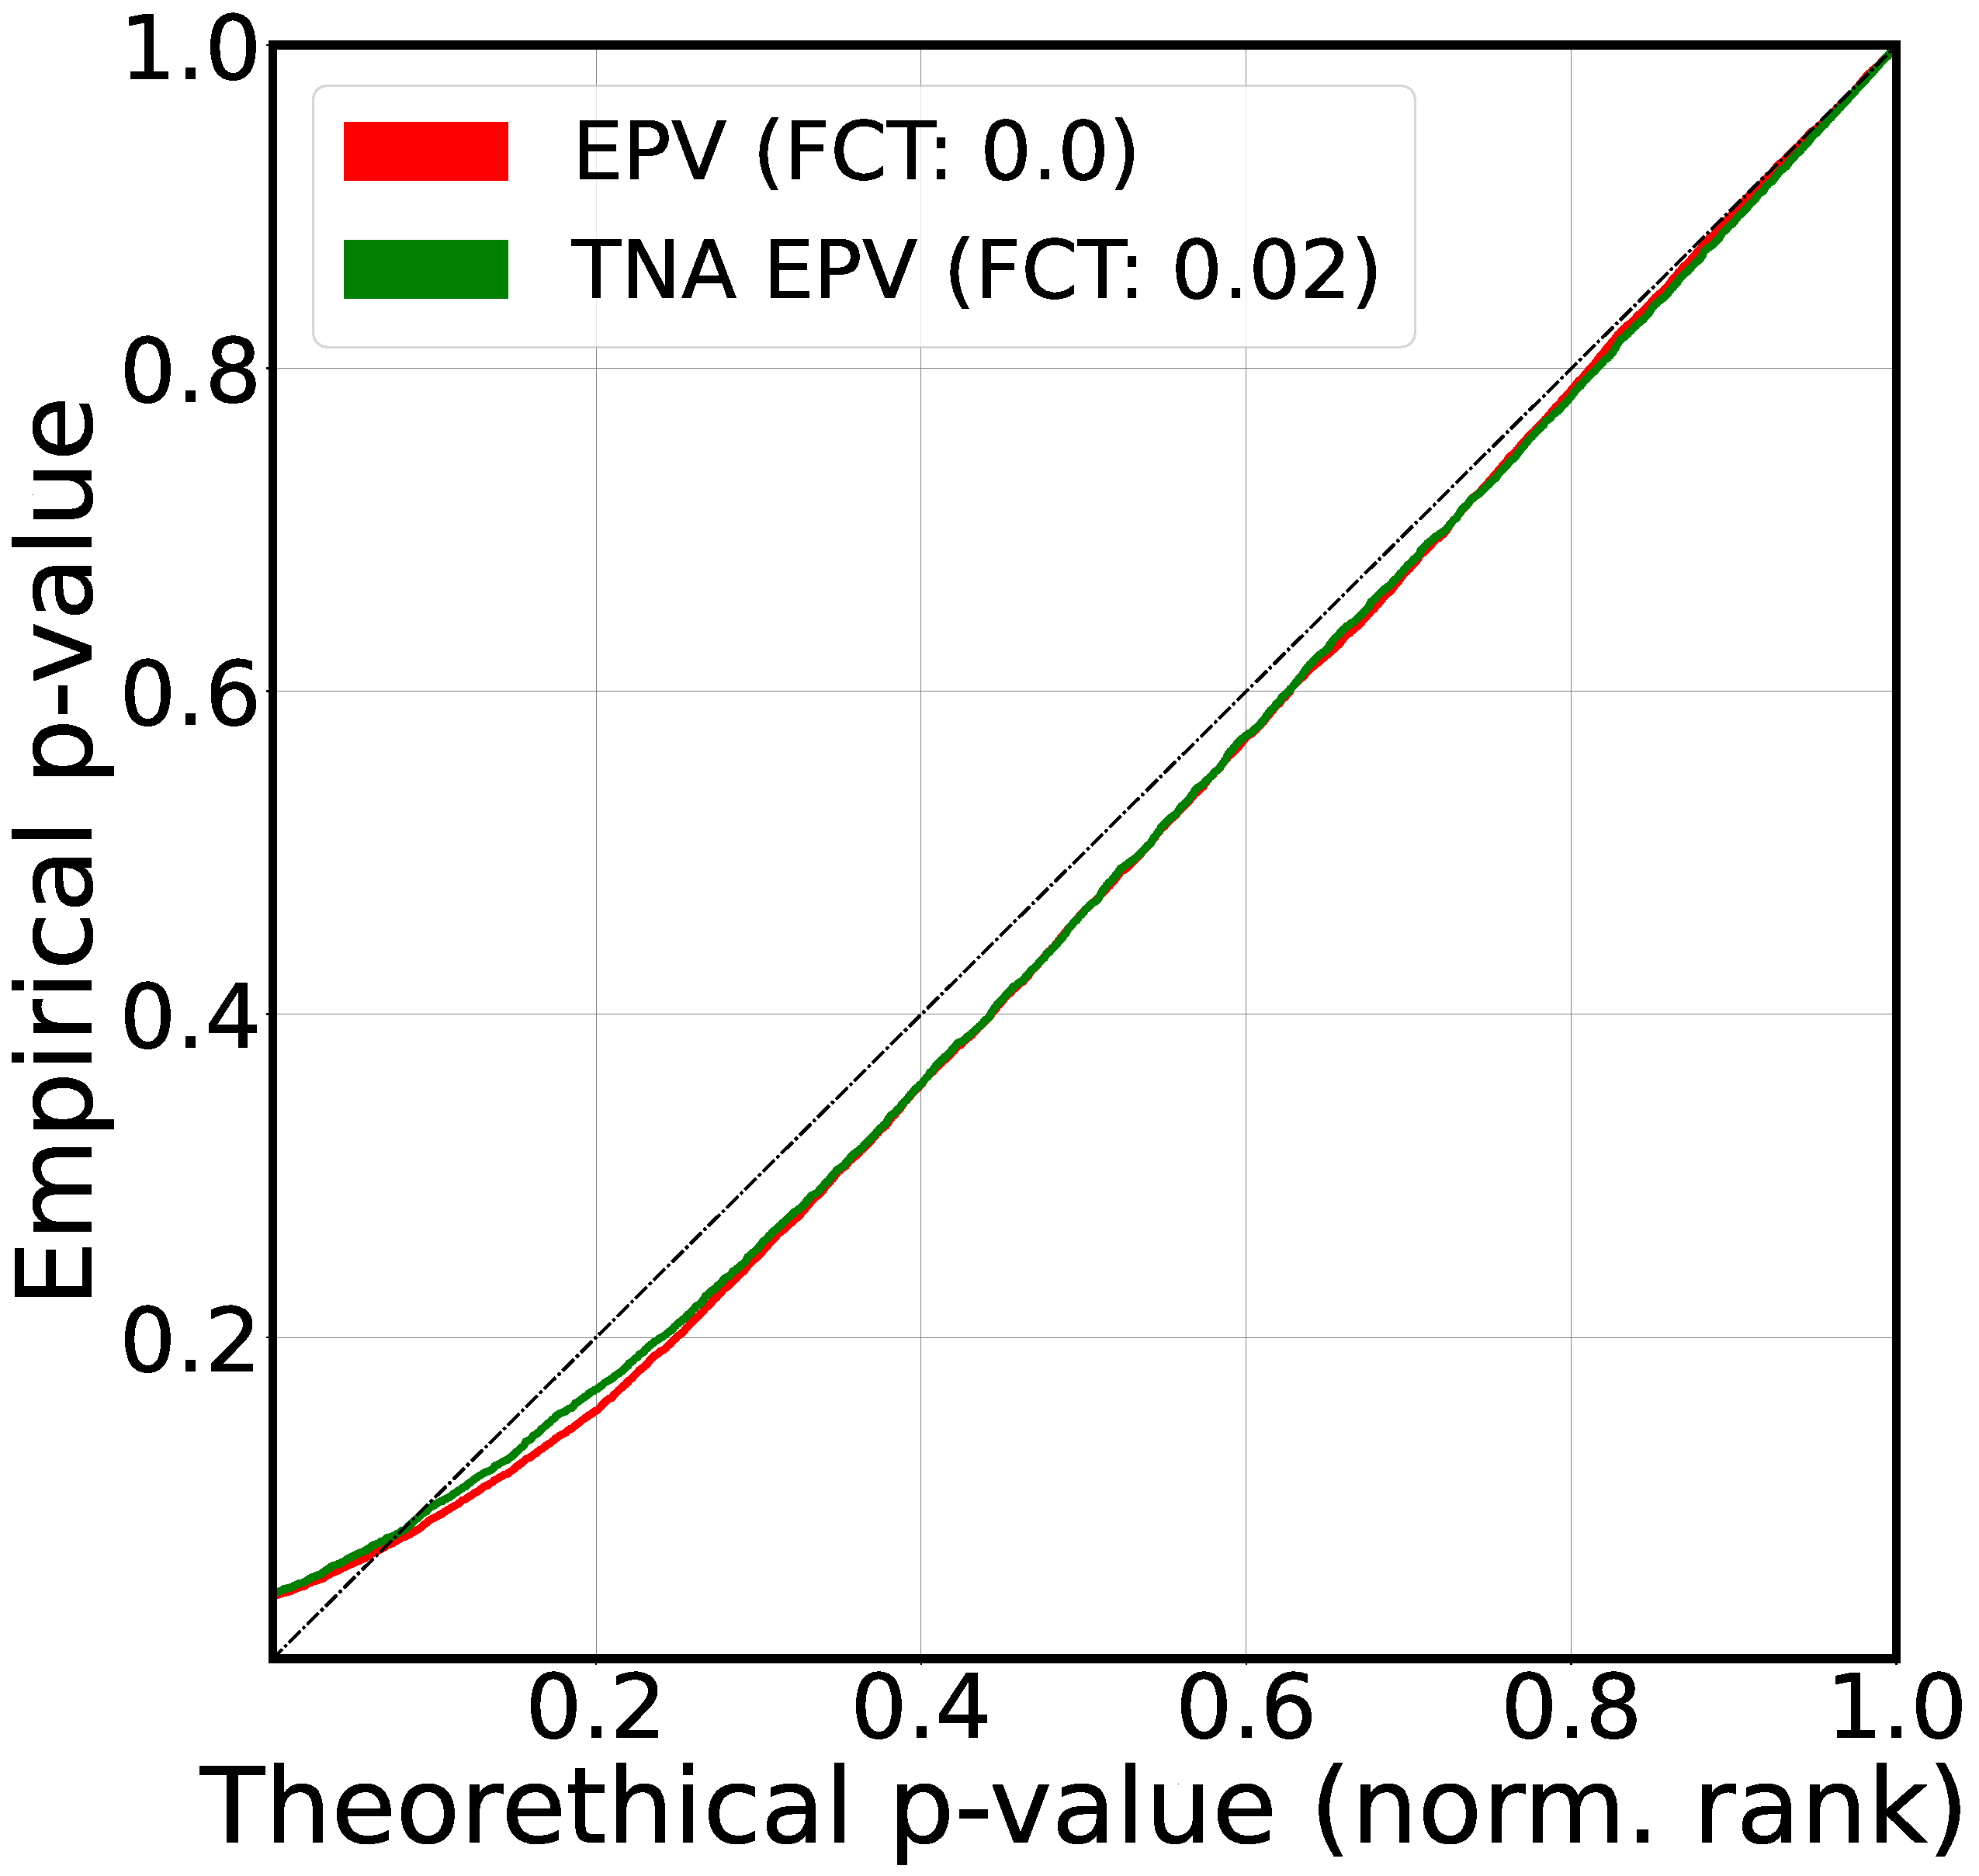
\includegraphics[width=1.7in]{img/cnn_QQ_pcam.pdf} &
		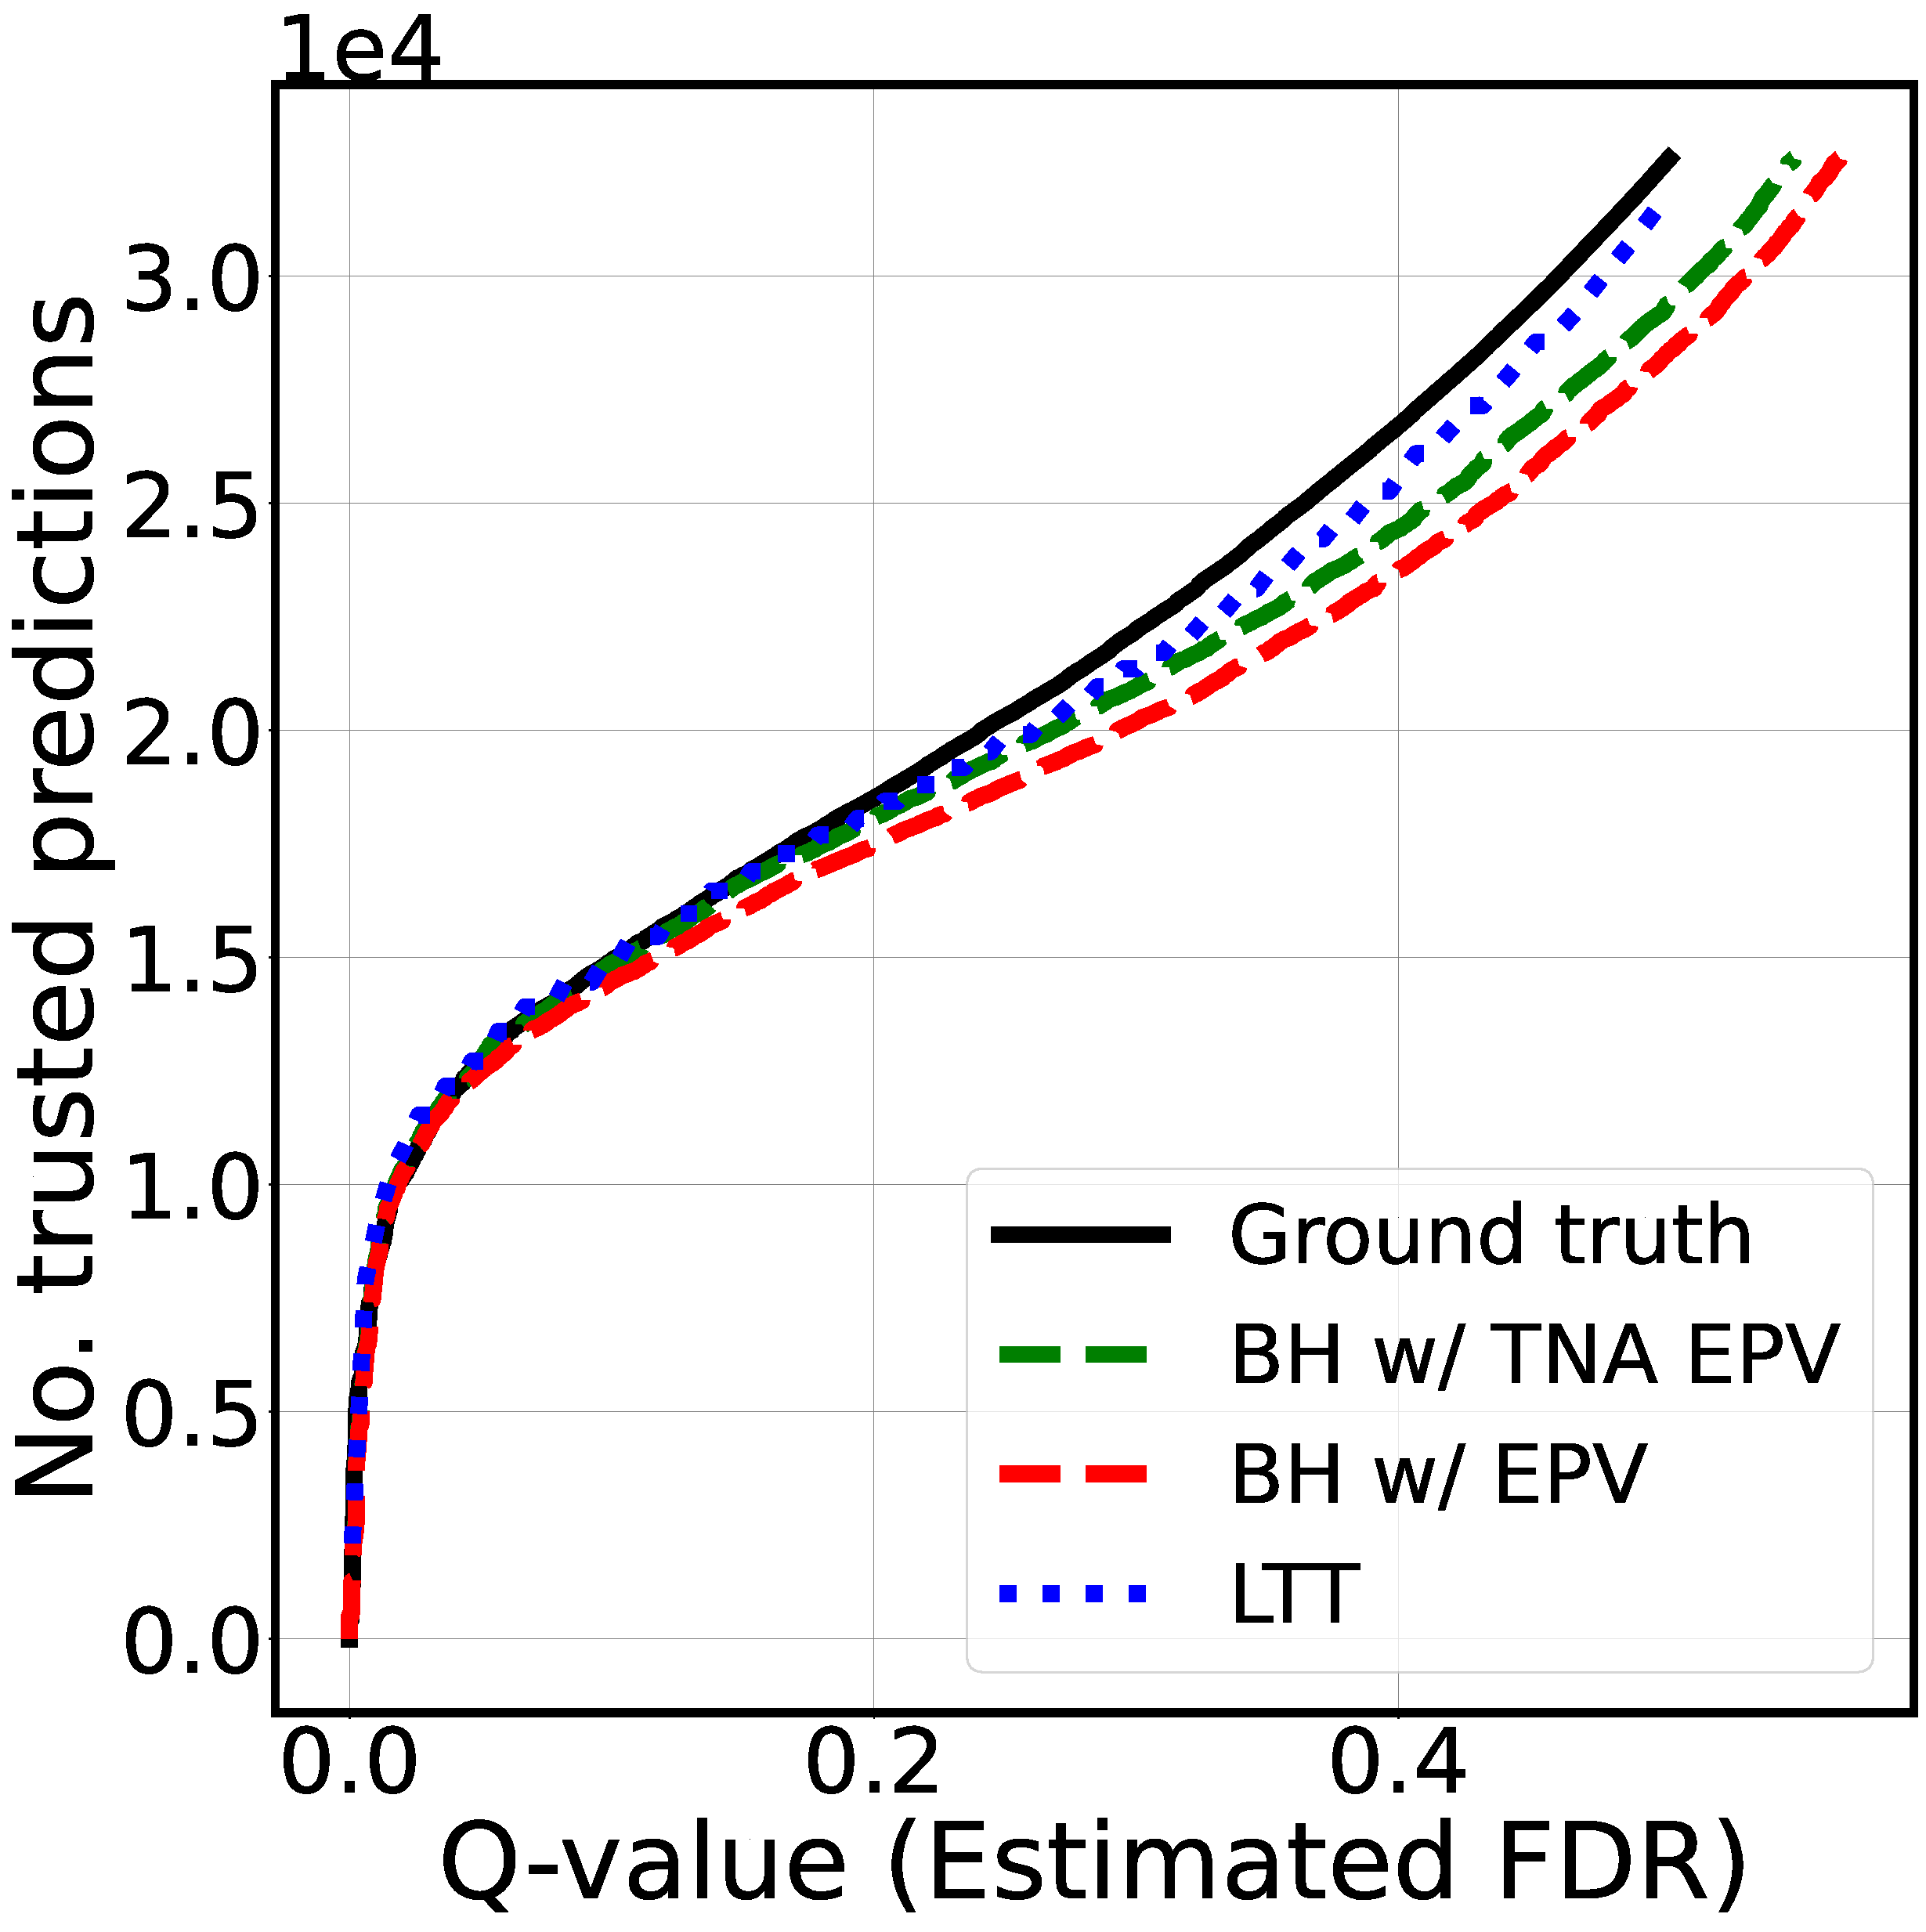
\includegraphics[width=1.7in]{img/cnn_pcam_fdr_control.pdf} & 
		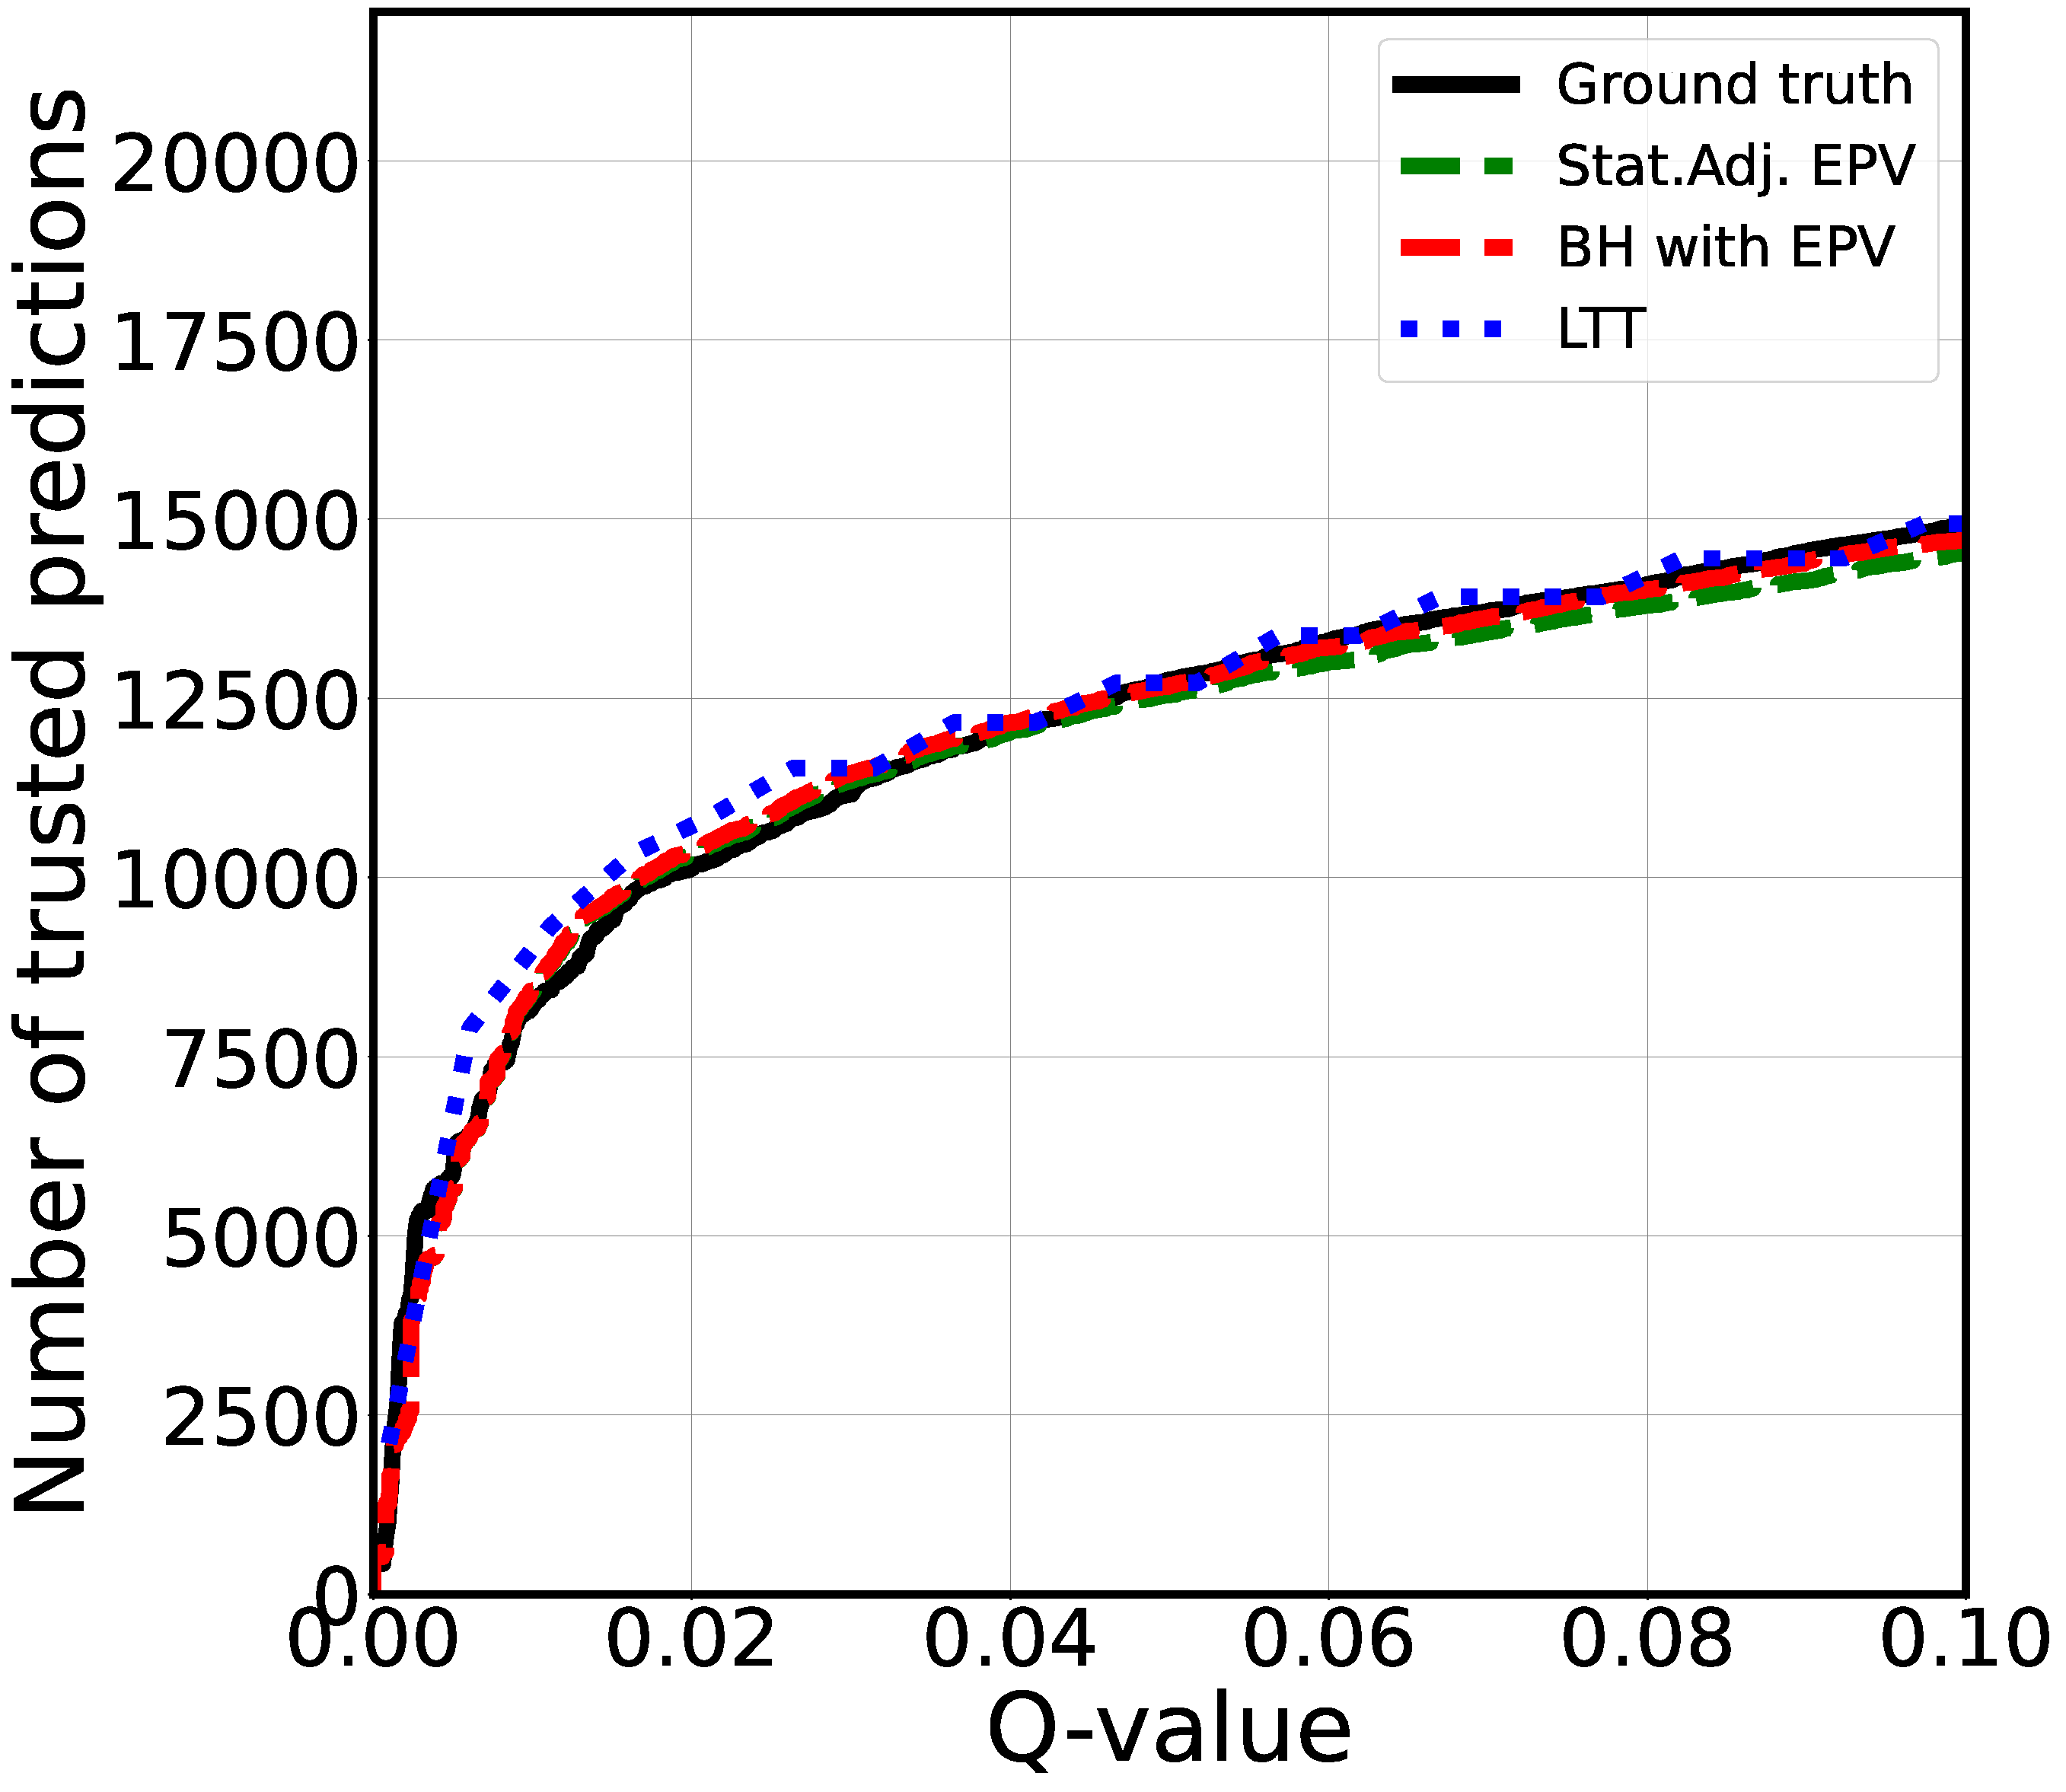
\includegraphics[width=1.7in]{img/cnn_pcam_fdr_control_loc.pdf} &
		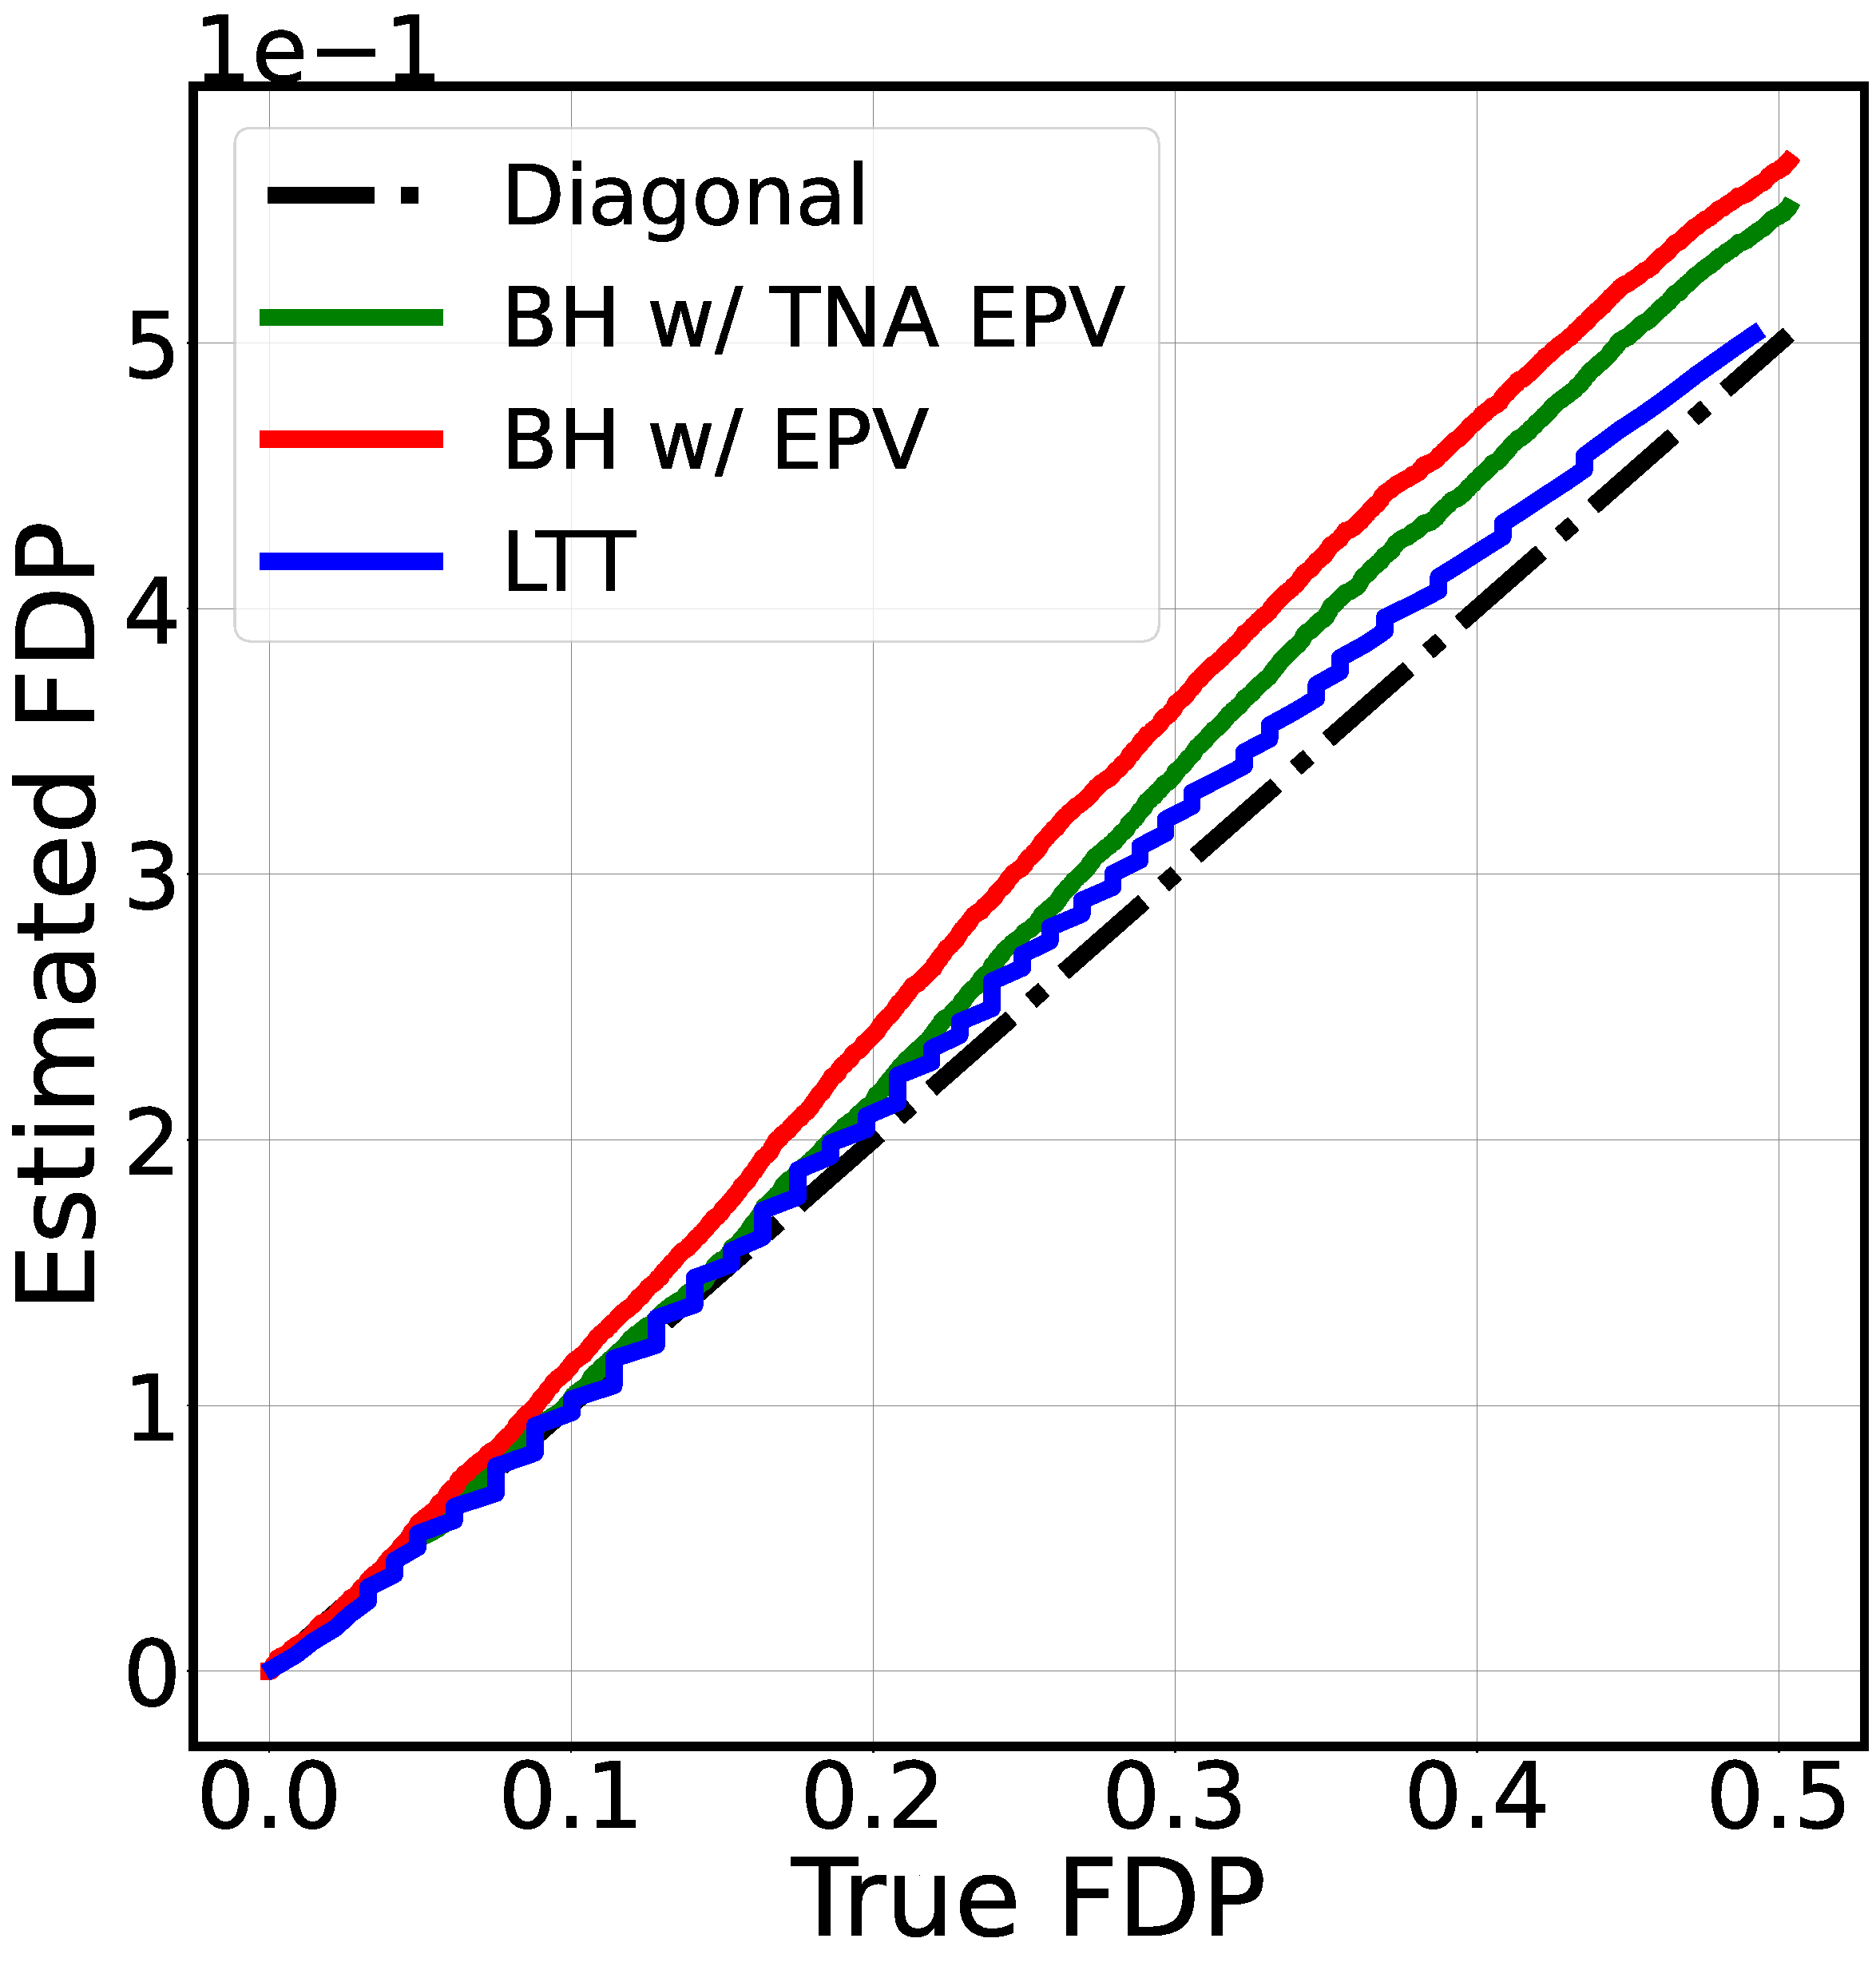
\includegraphics[width=1.7in]{img/cnn_FDPscat_pcam.pdf}\\	
		\multicolumn{4}{l}{\bf (ii) PCam with class distribution shift.:}\\		
		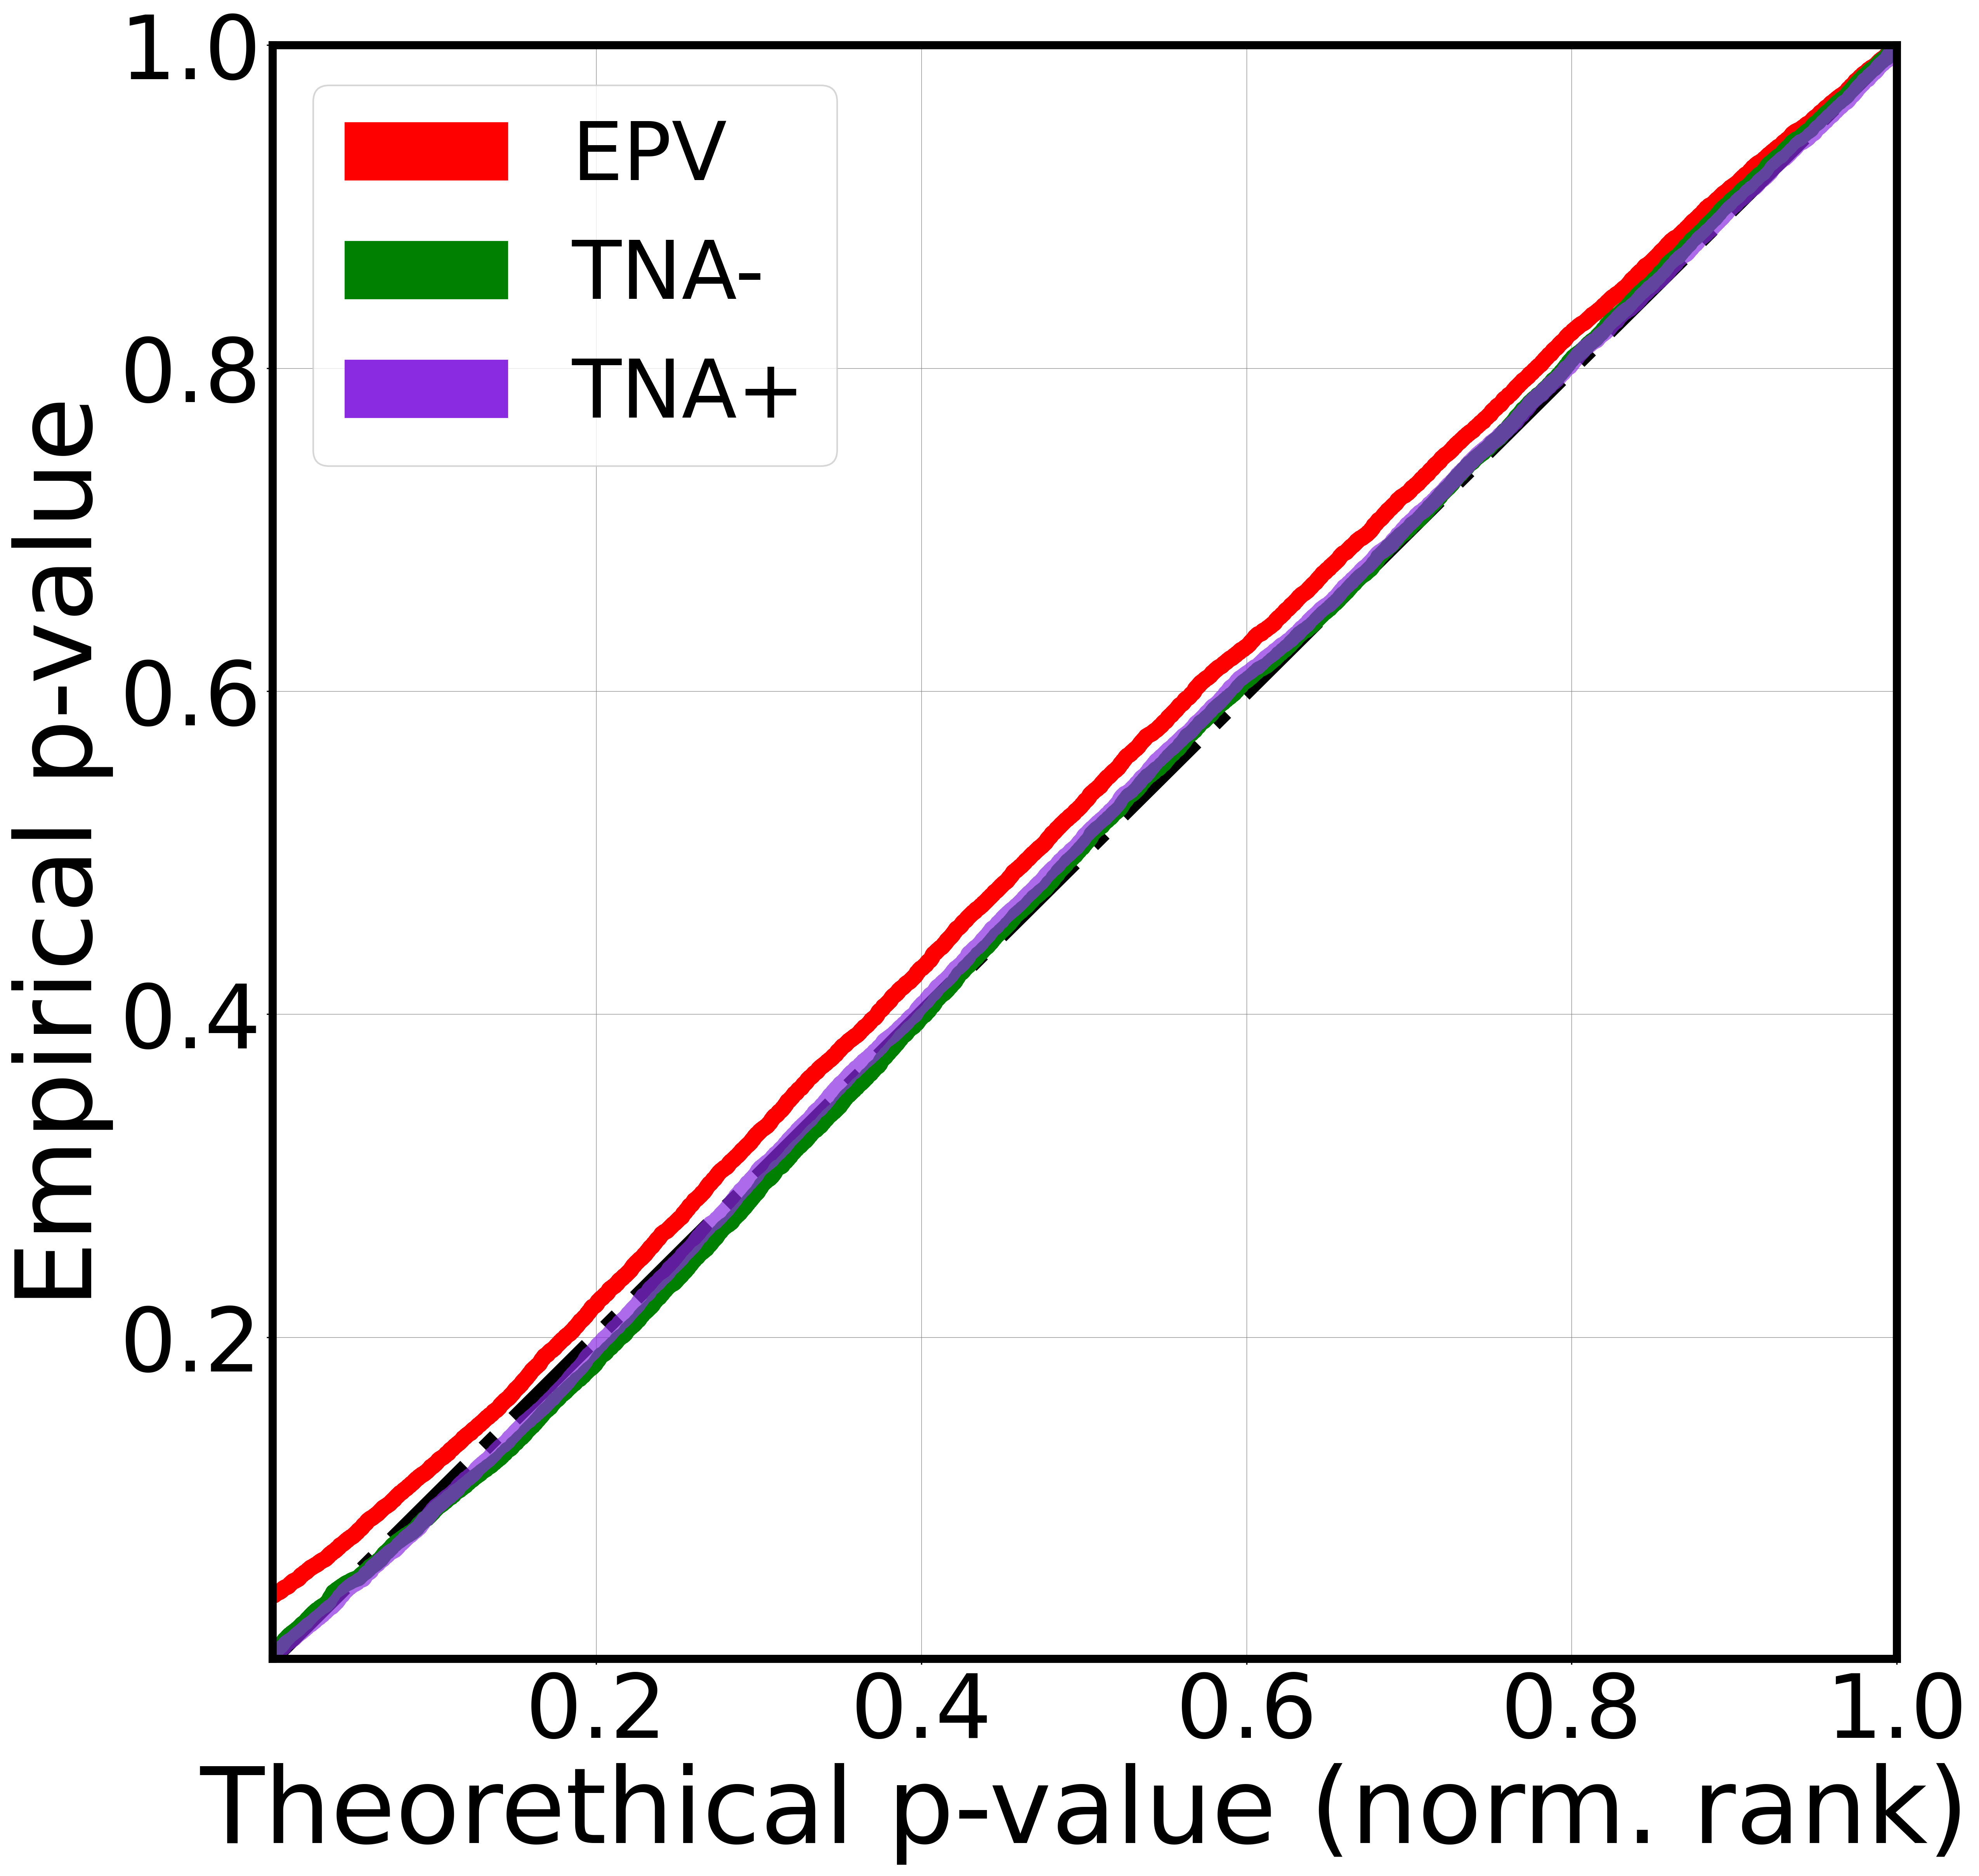
\includegraphics[width=1.7in]{img/cnn_QQ_pcam_balanced.png} &
		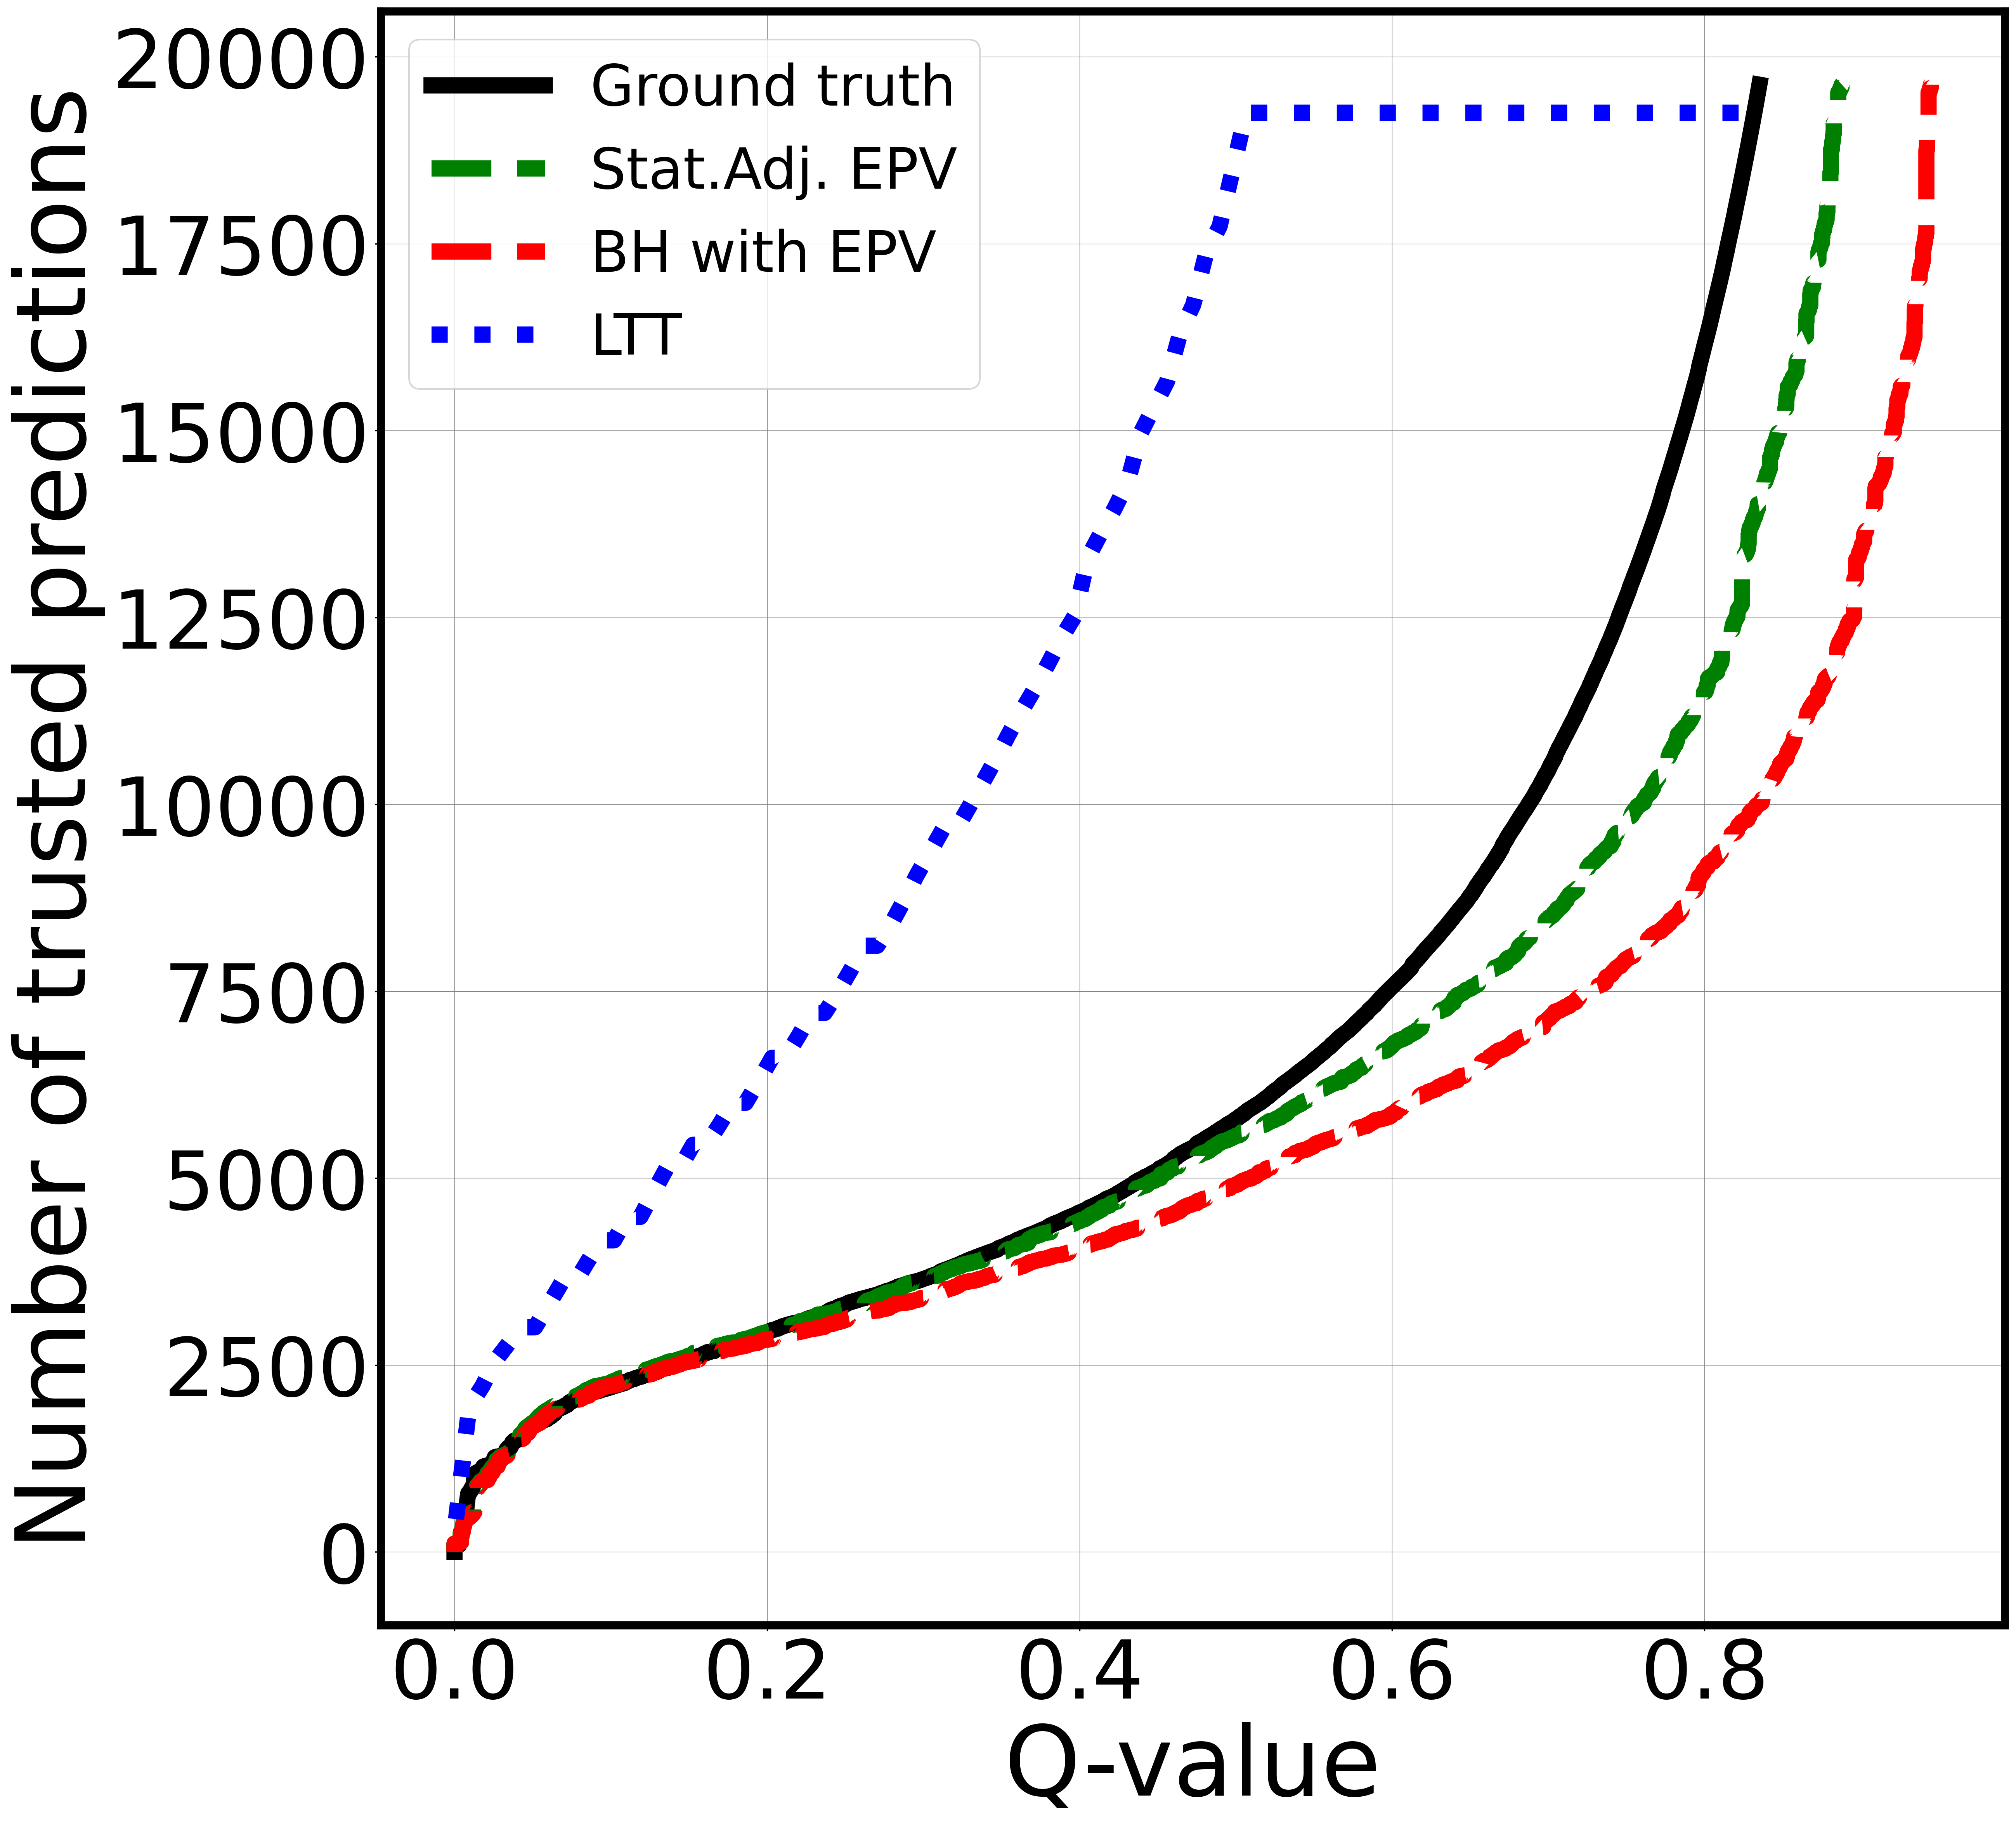
\includegraphics[width=1.7in]{img/cnn_pcam_balanced_fdr_control.png} & 
		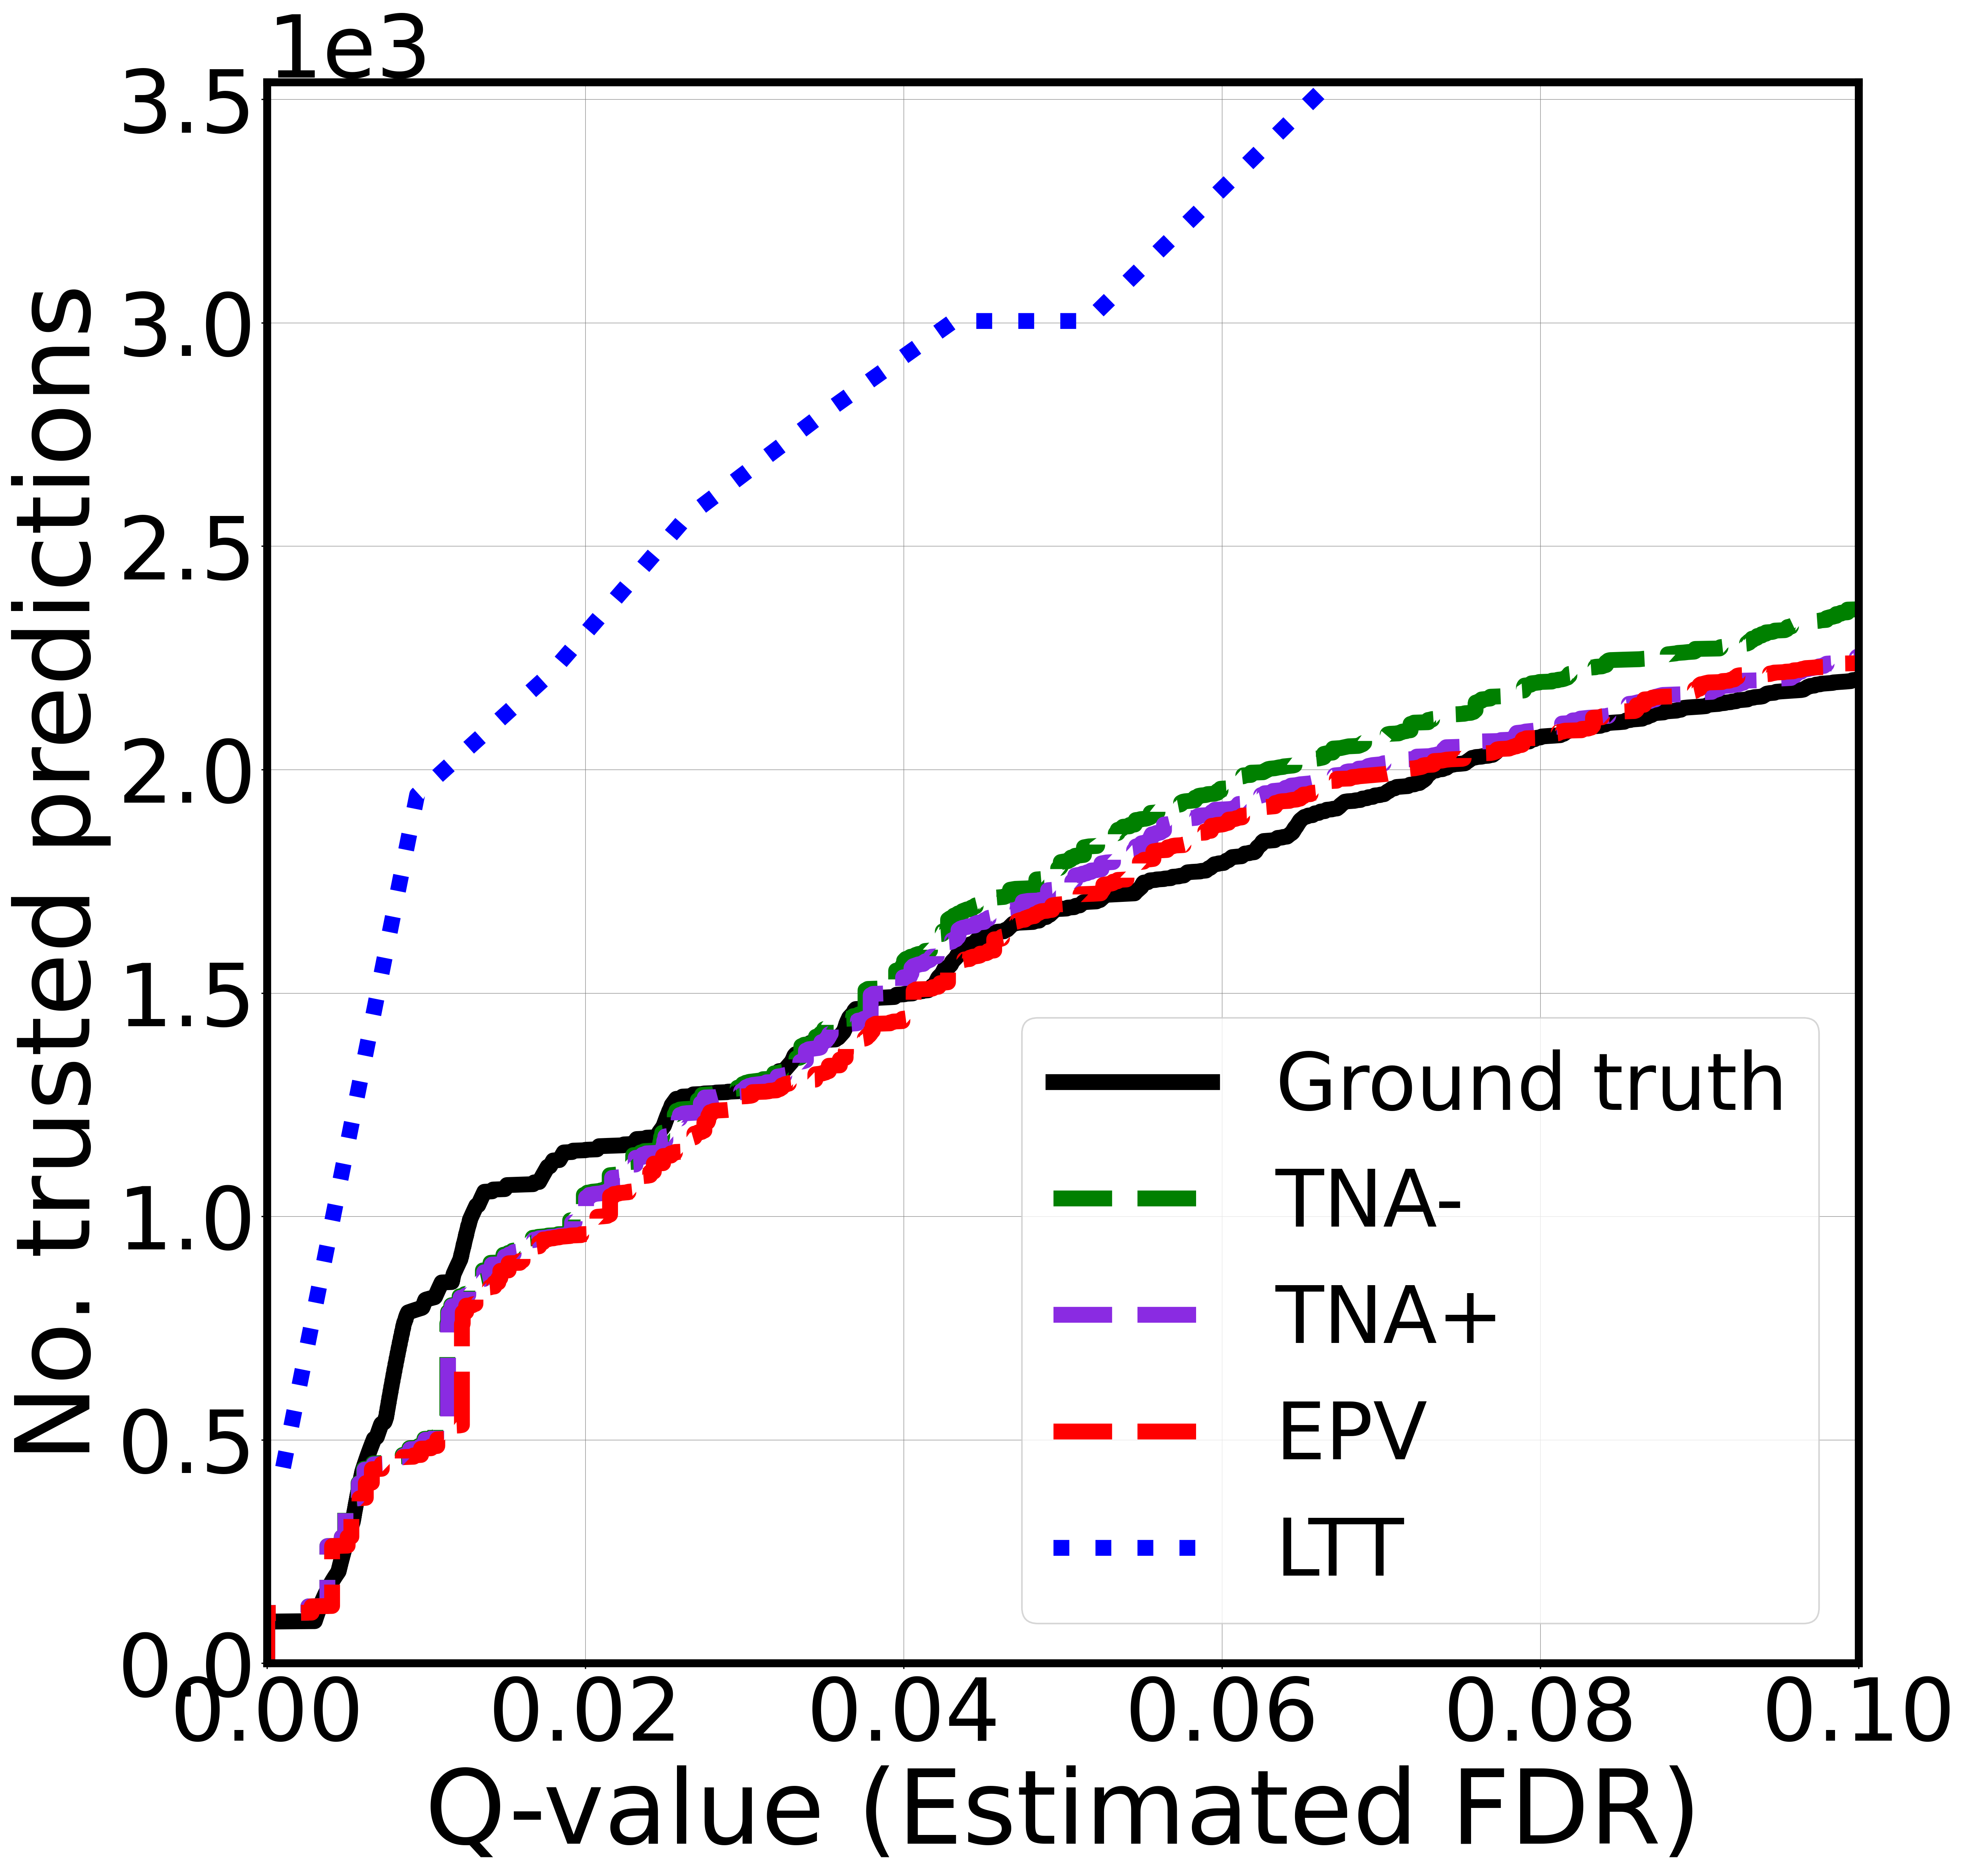
\includegraphics[width=1.7in]{img/cnn_pcam_balanced_fdr_control_loc.png} &
		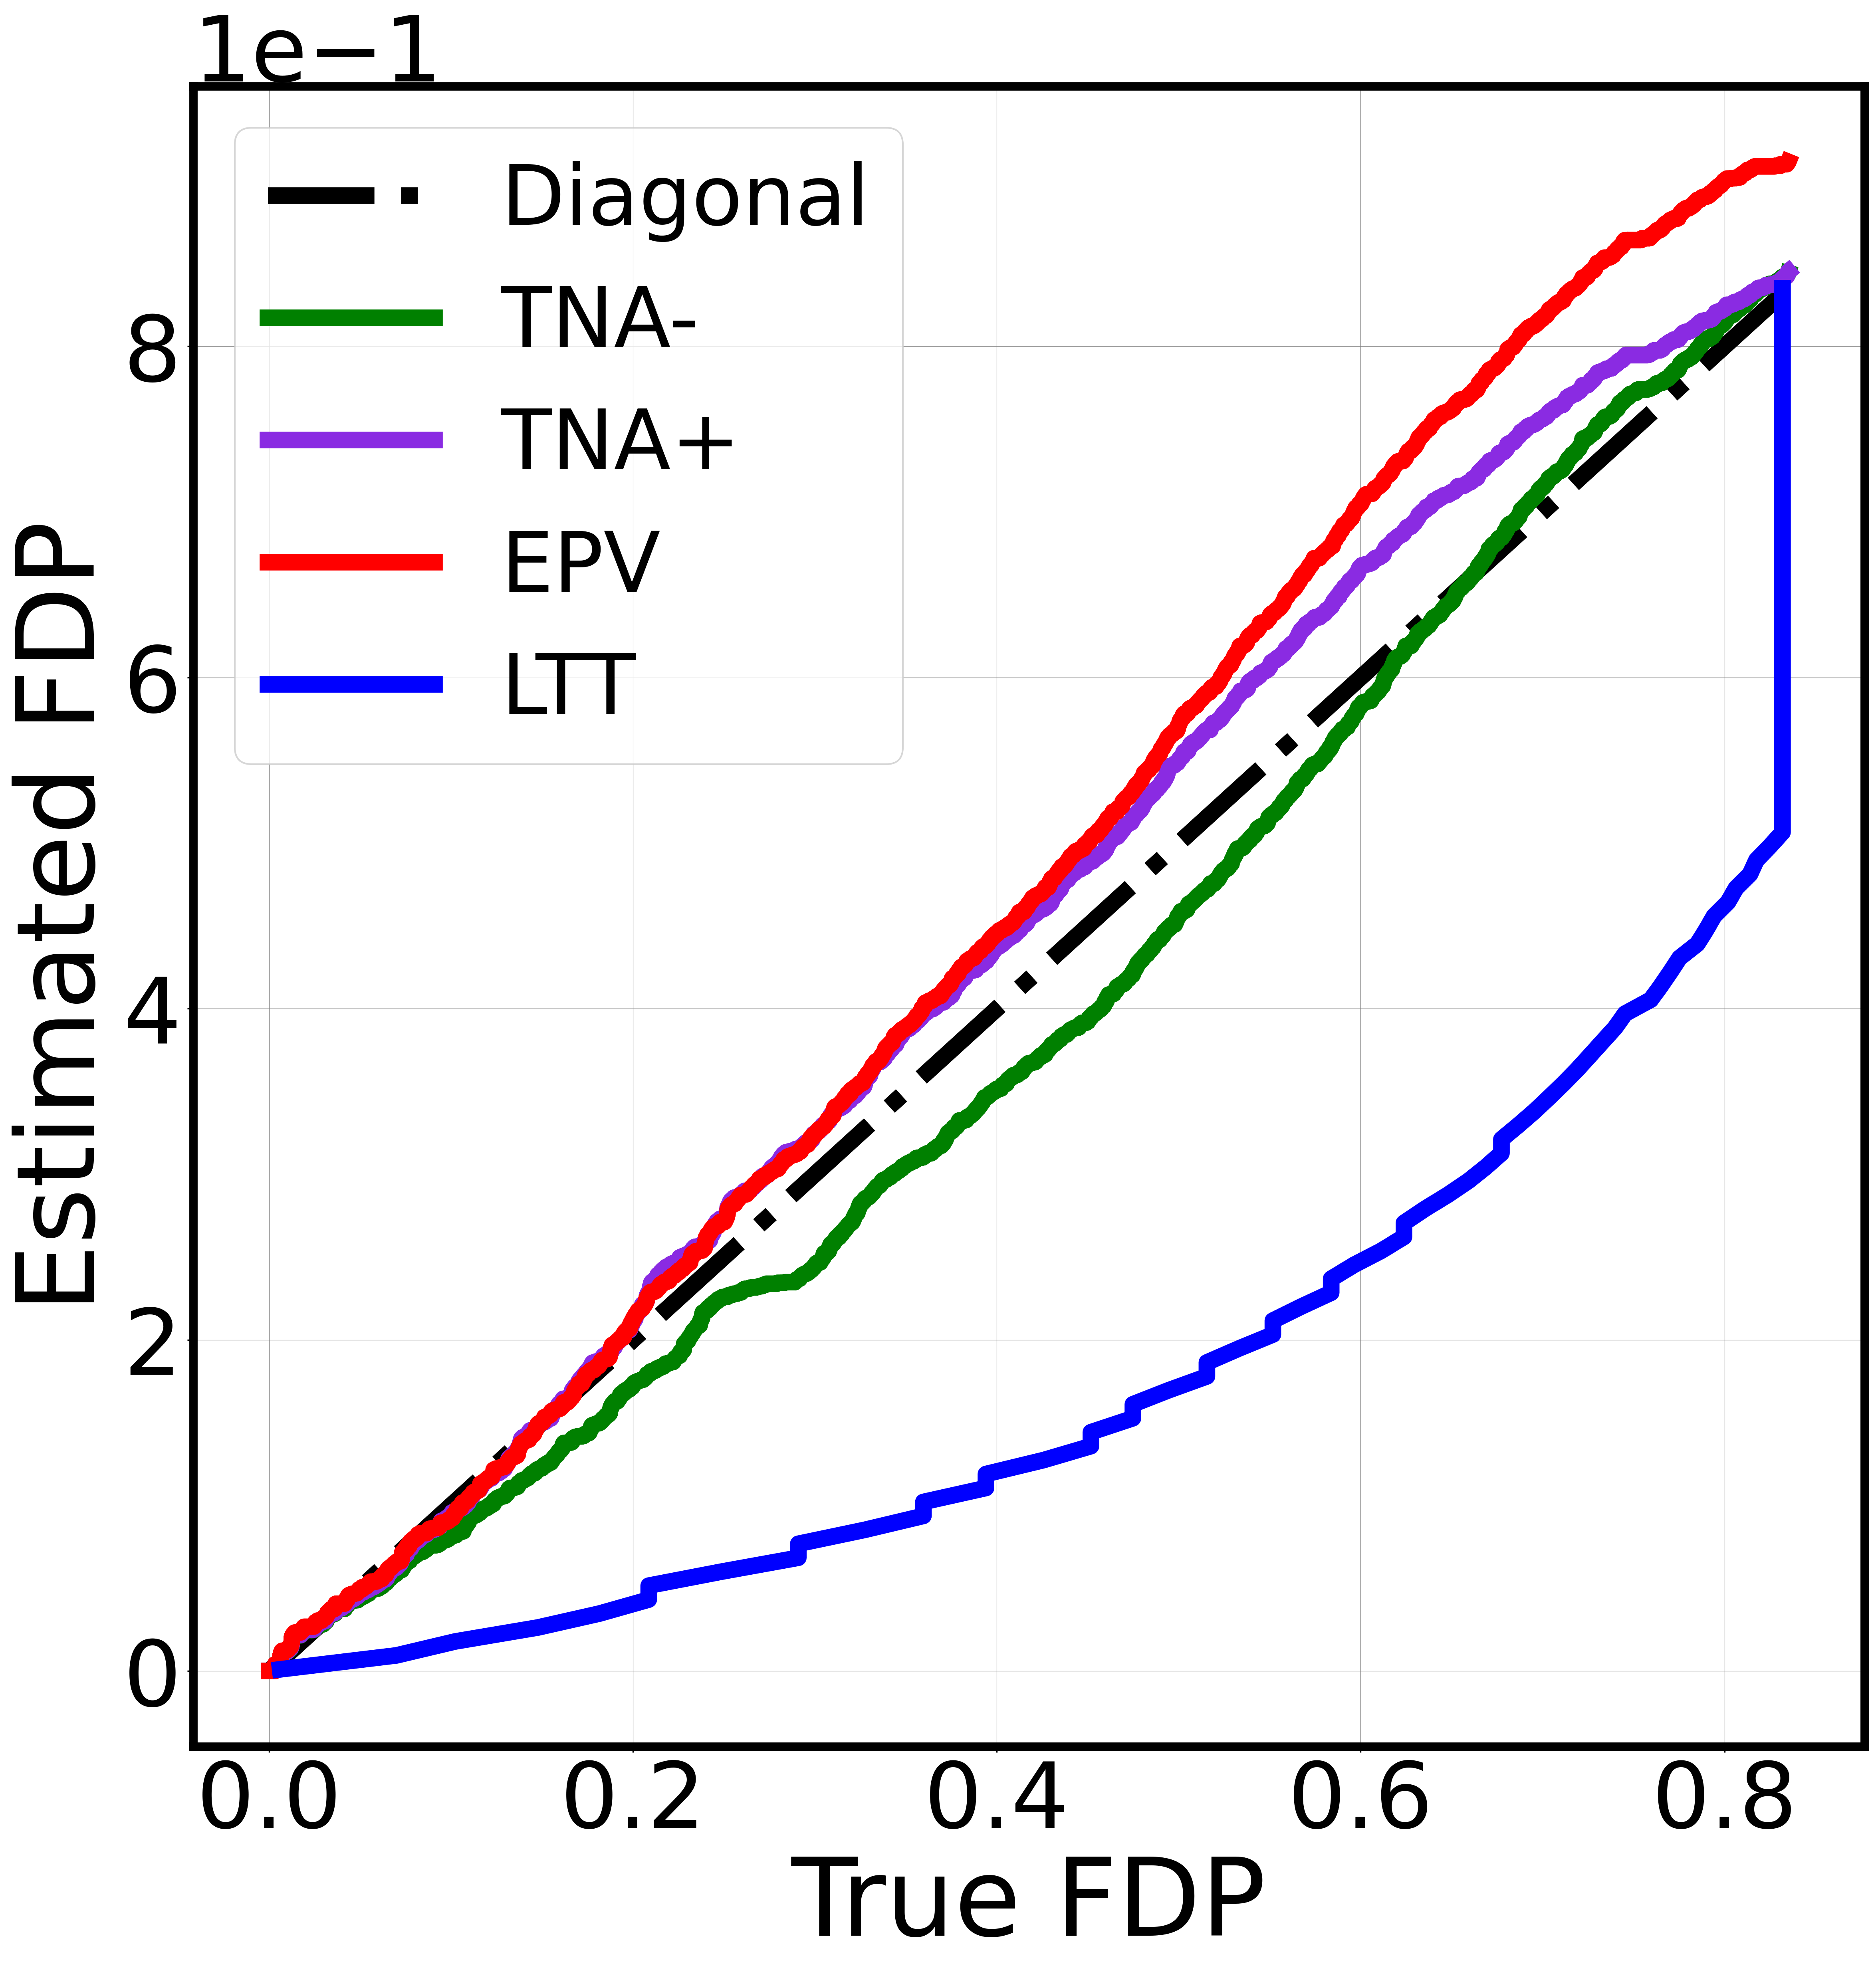
\includegraphics[width=1.7in]{img/cnn_FDPscat_pcam_balanced.png}\\
		\multicolumn{4}{l}{\bf (iii) Standard TissueNet dataset:}\\		
		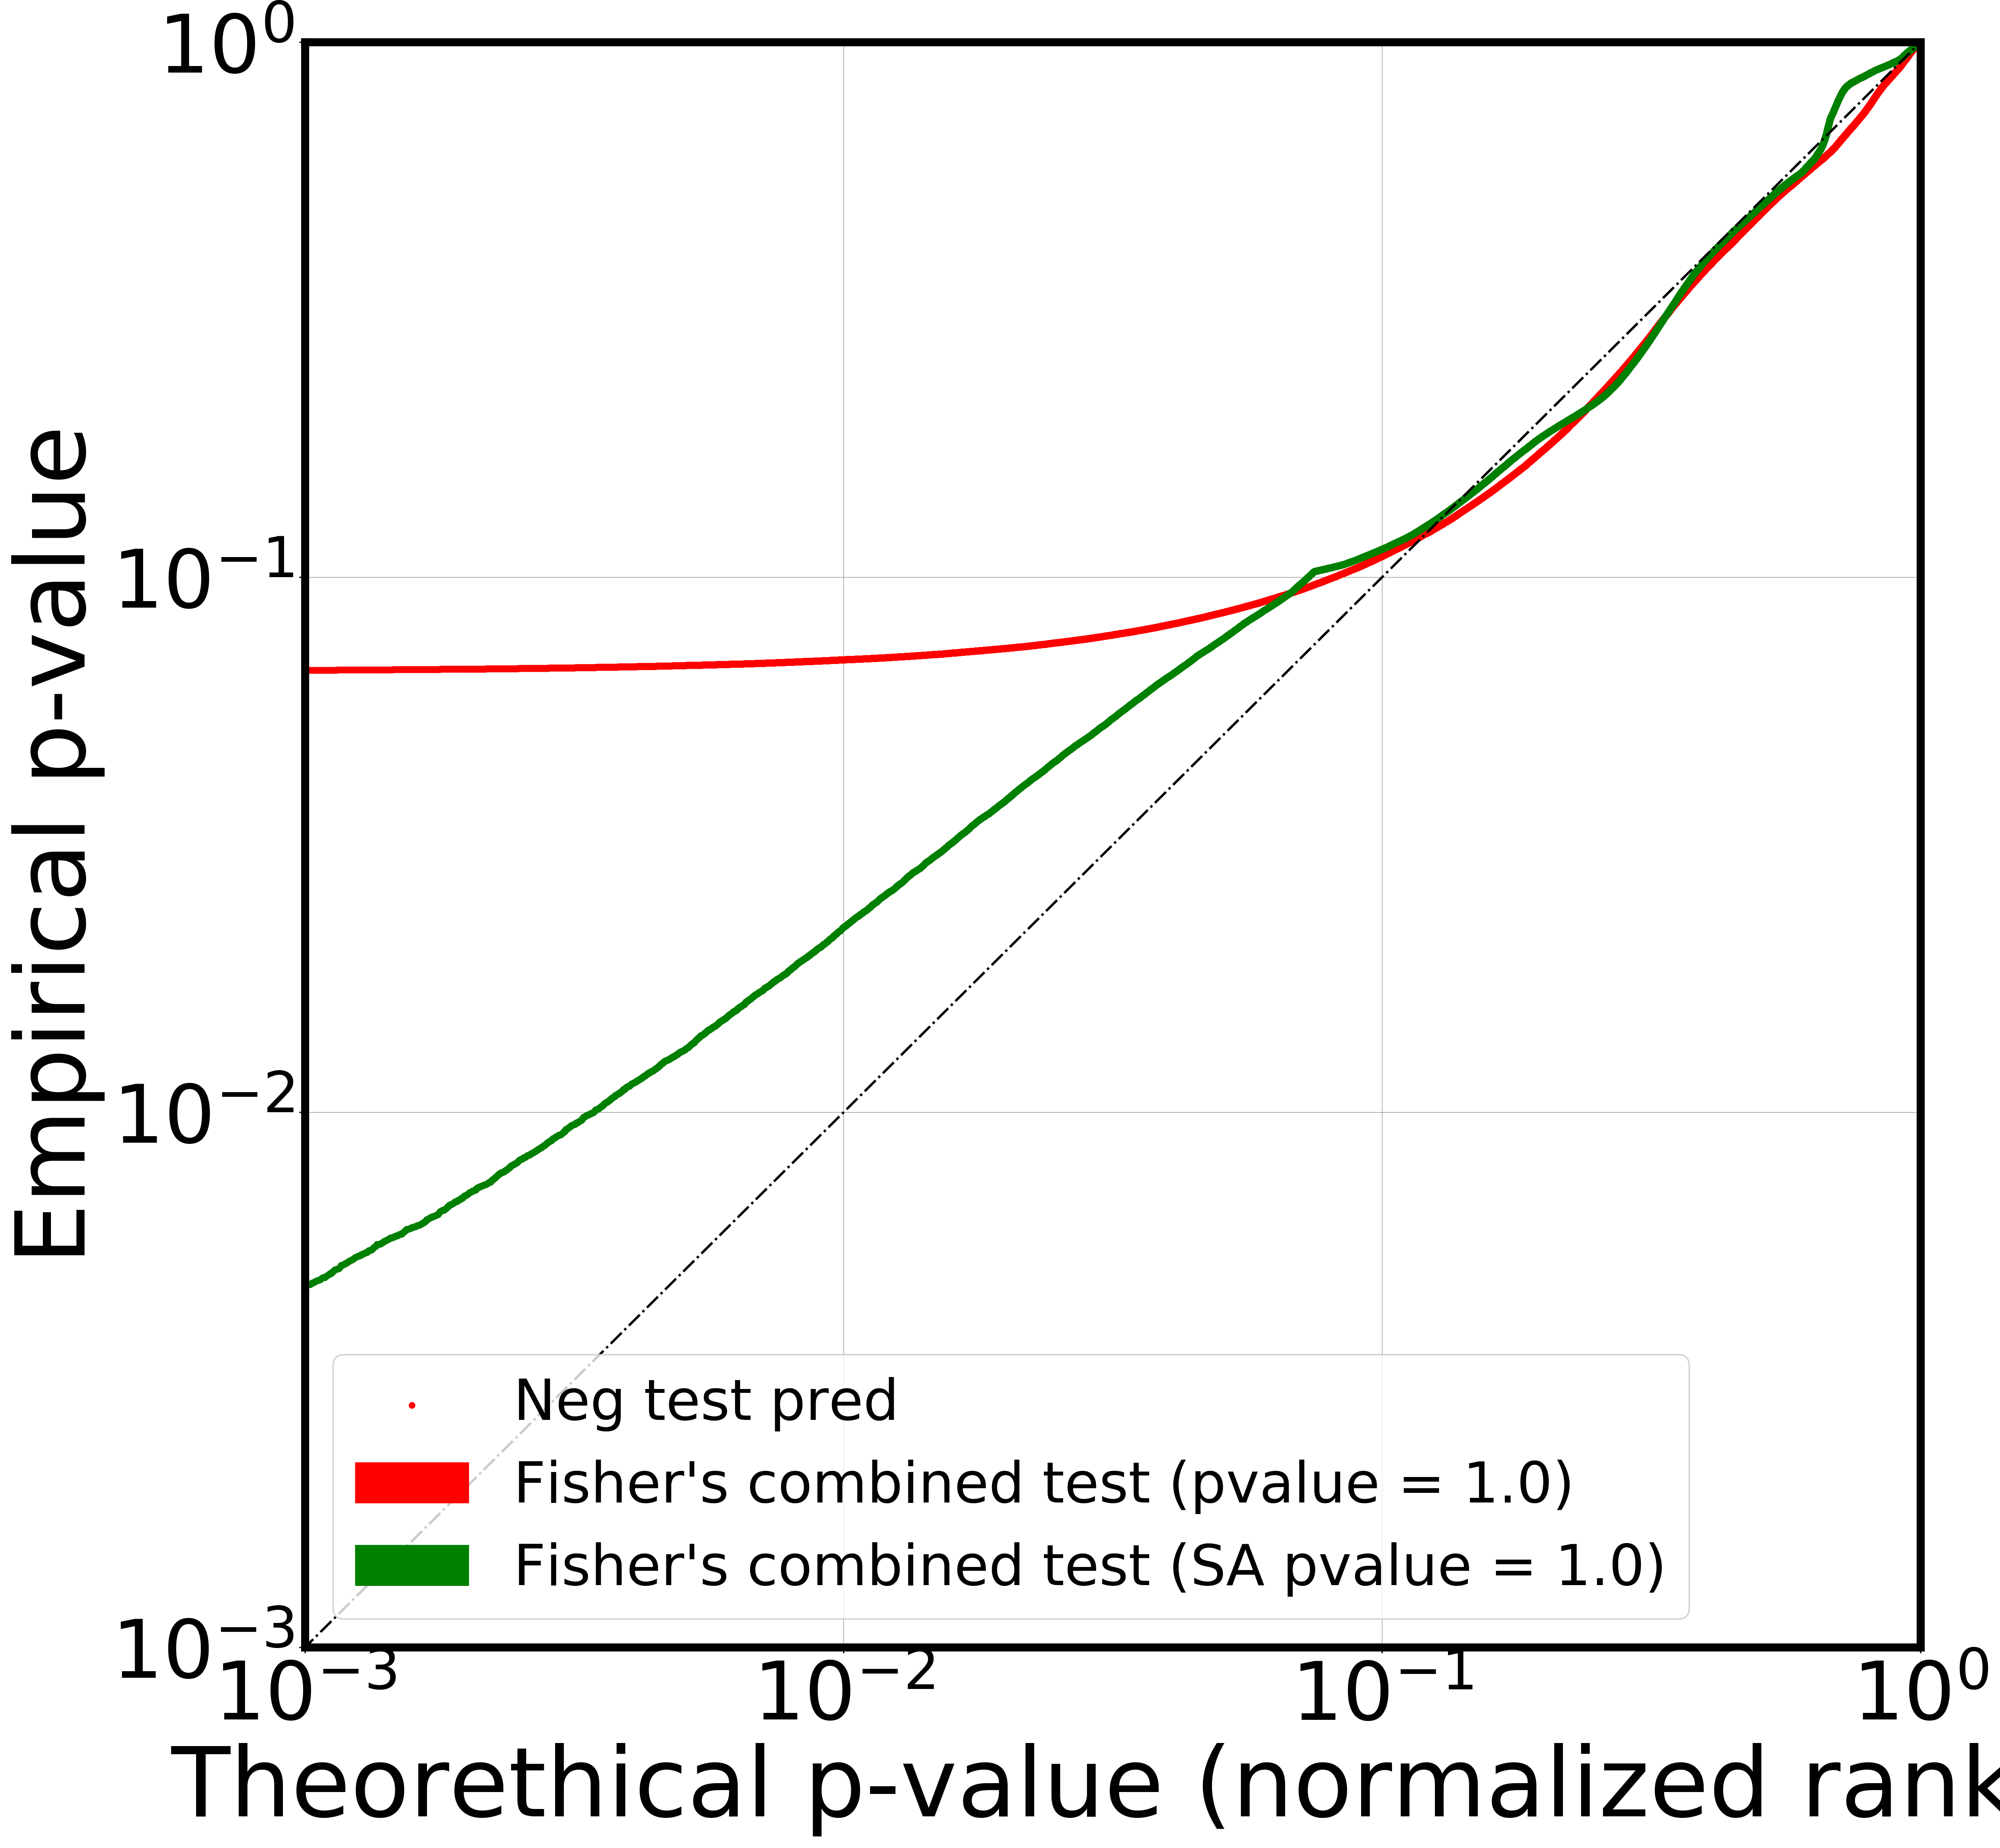
\includegraphics[width=1.7in]{img/cnn_QQ_cells_segment_TA_log.png} &
		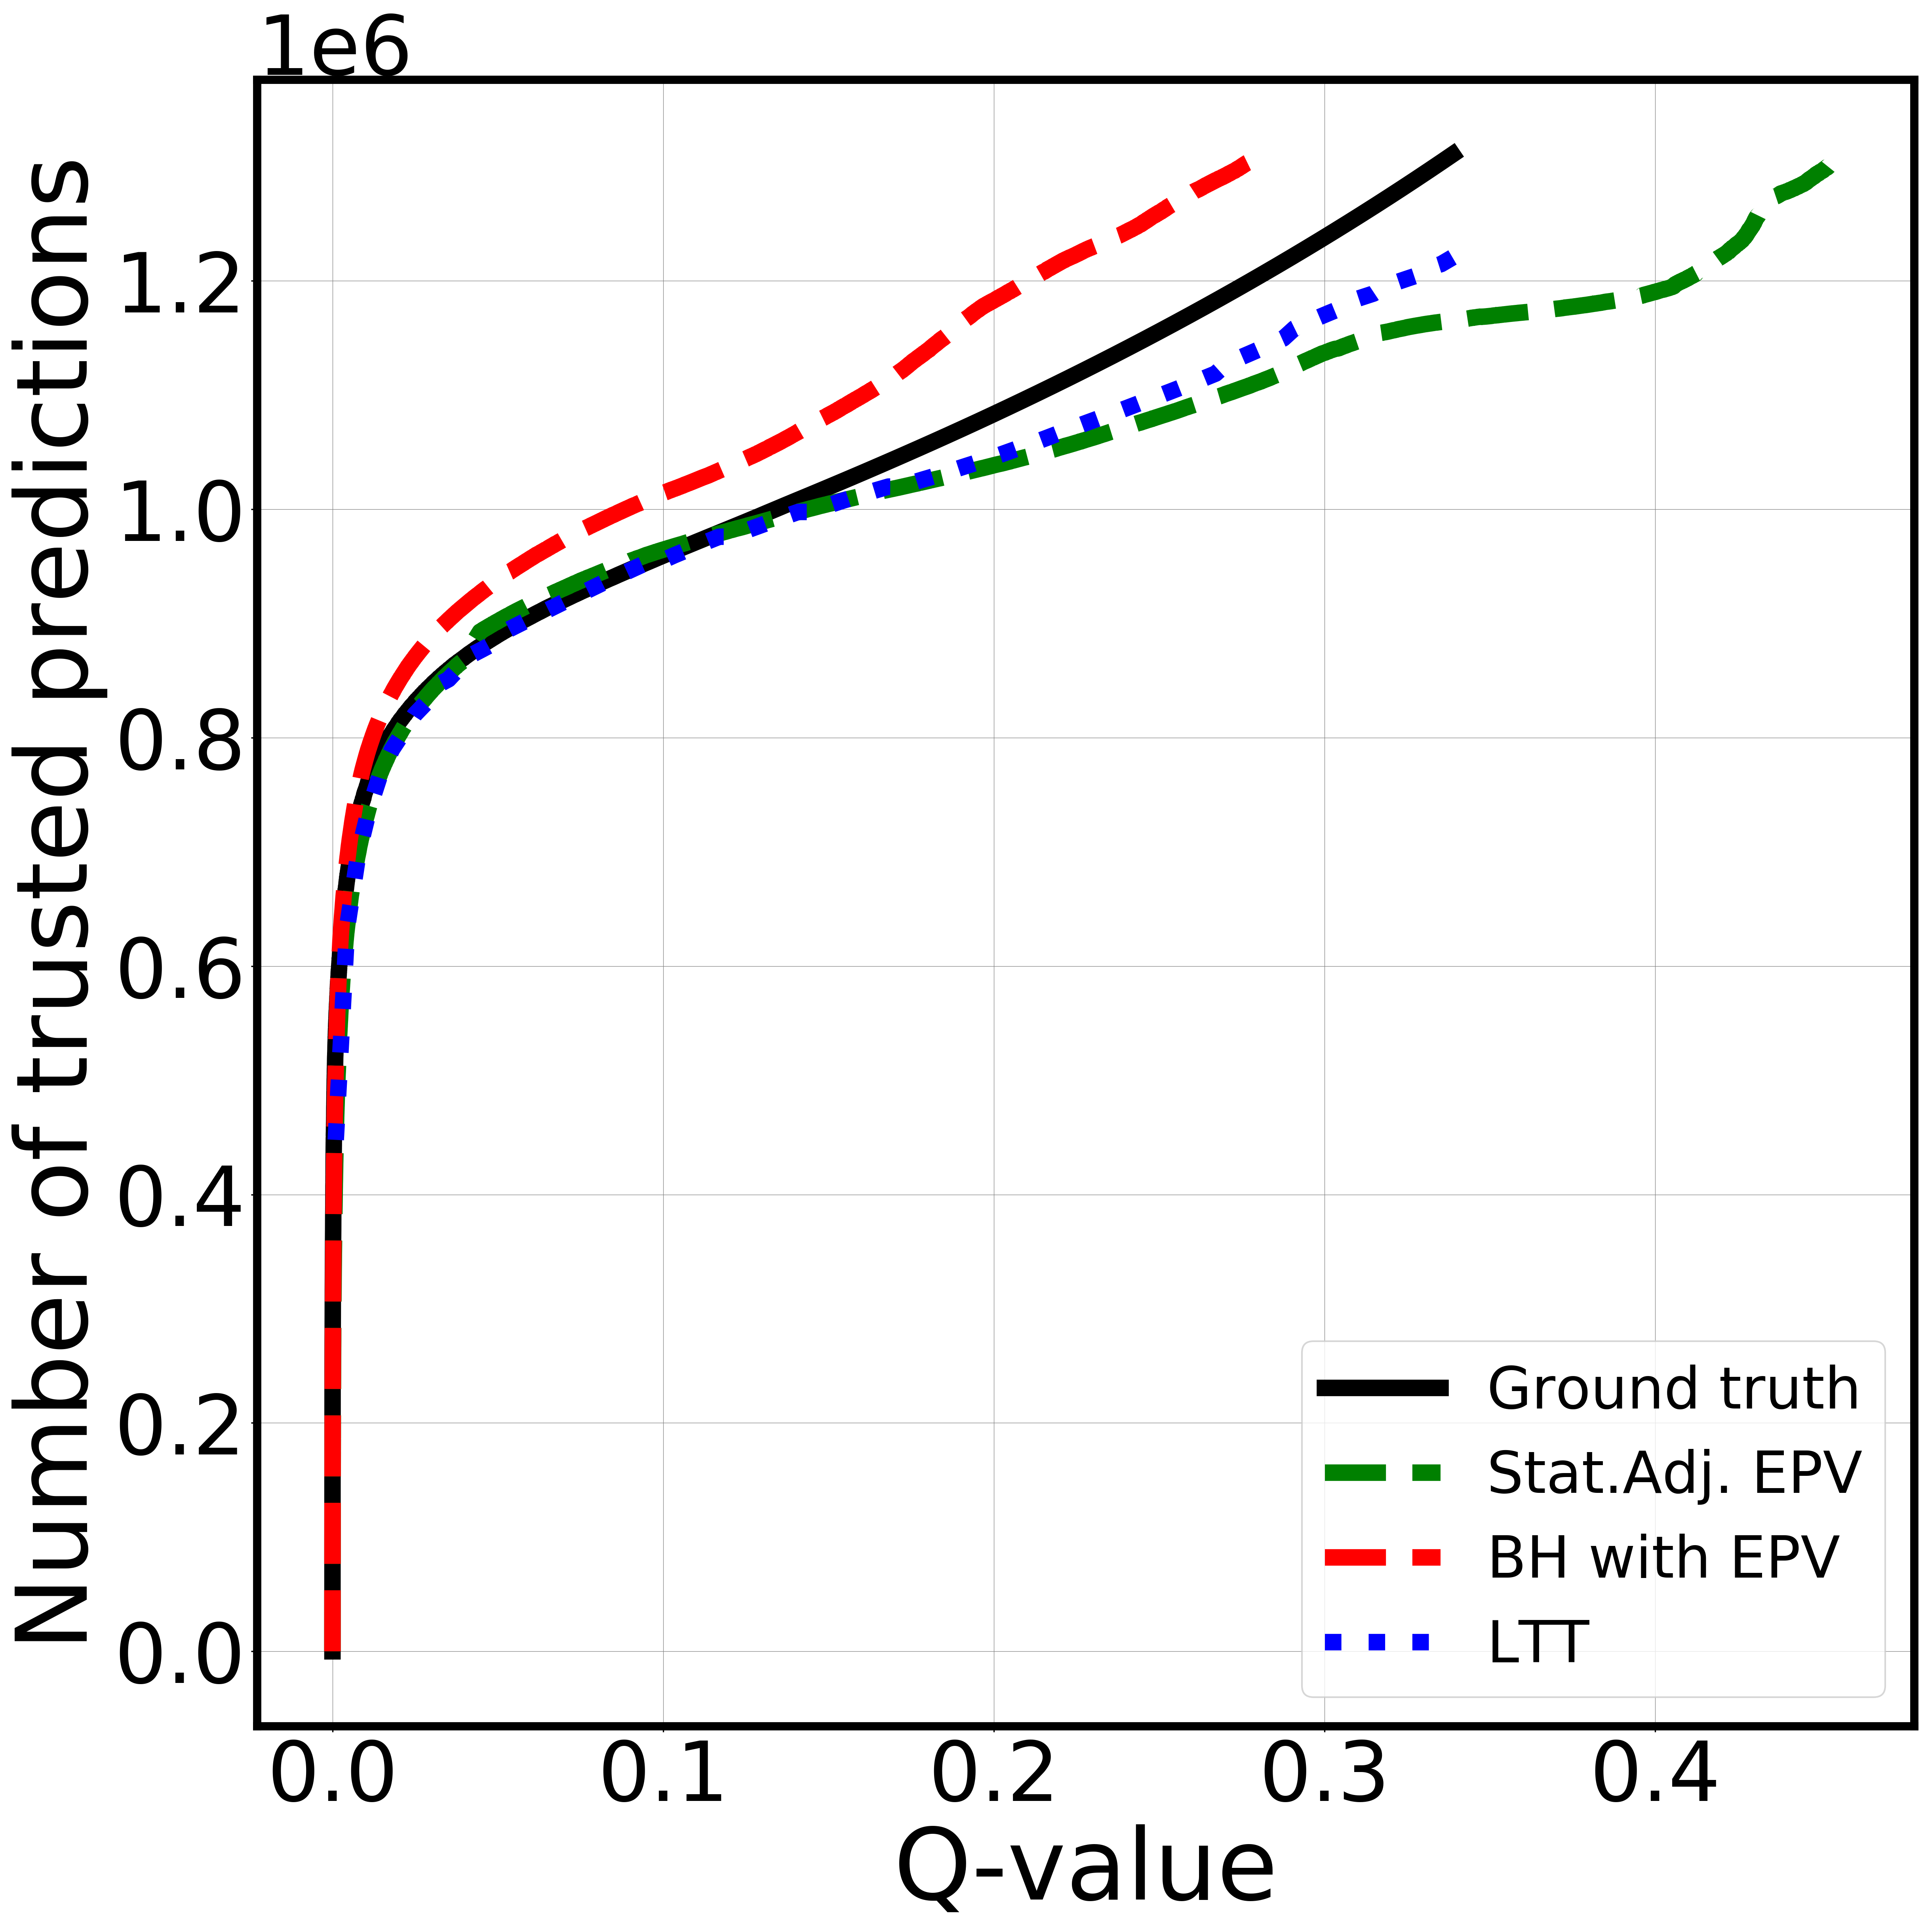
\includegraphics[width=1.7in]{img/cnn_cells_segment_TA_fdr_control.png} & 
		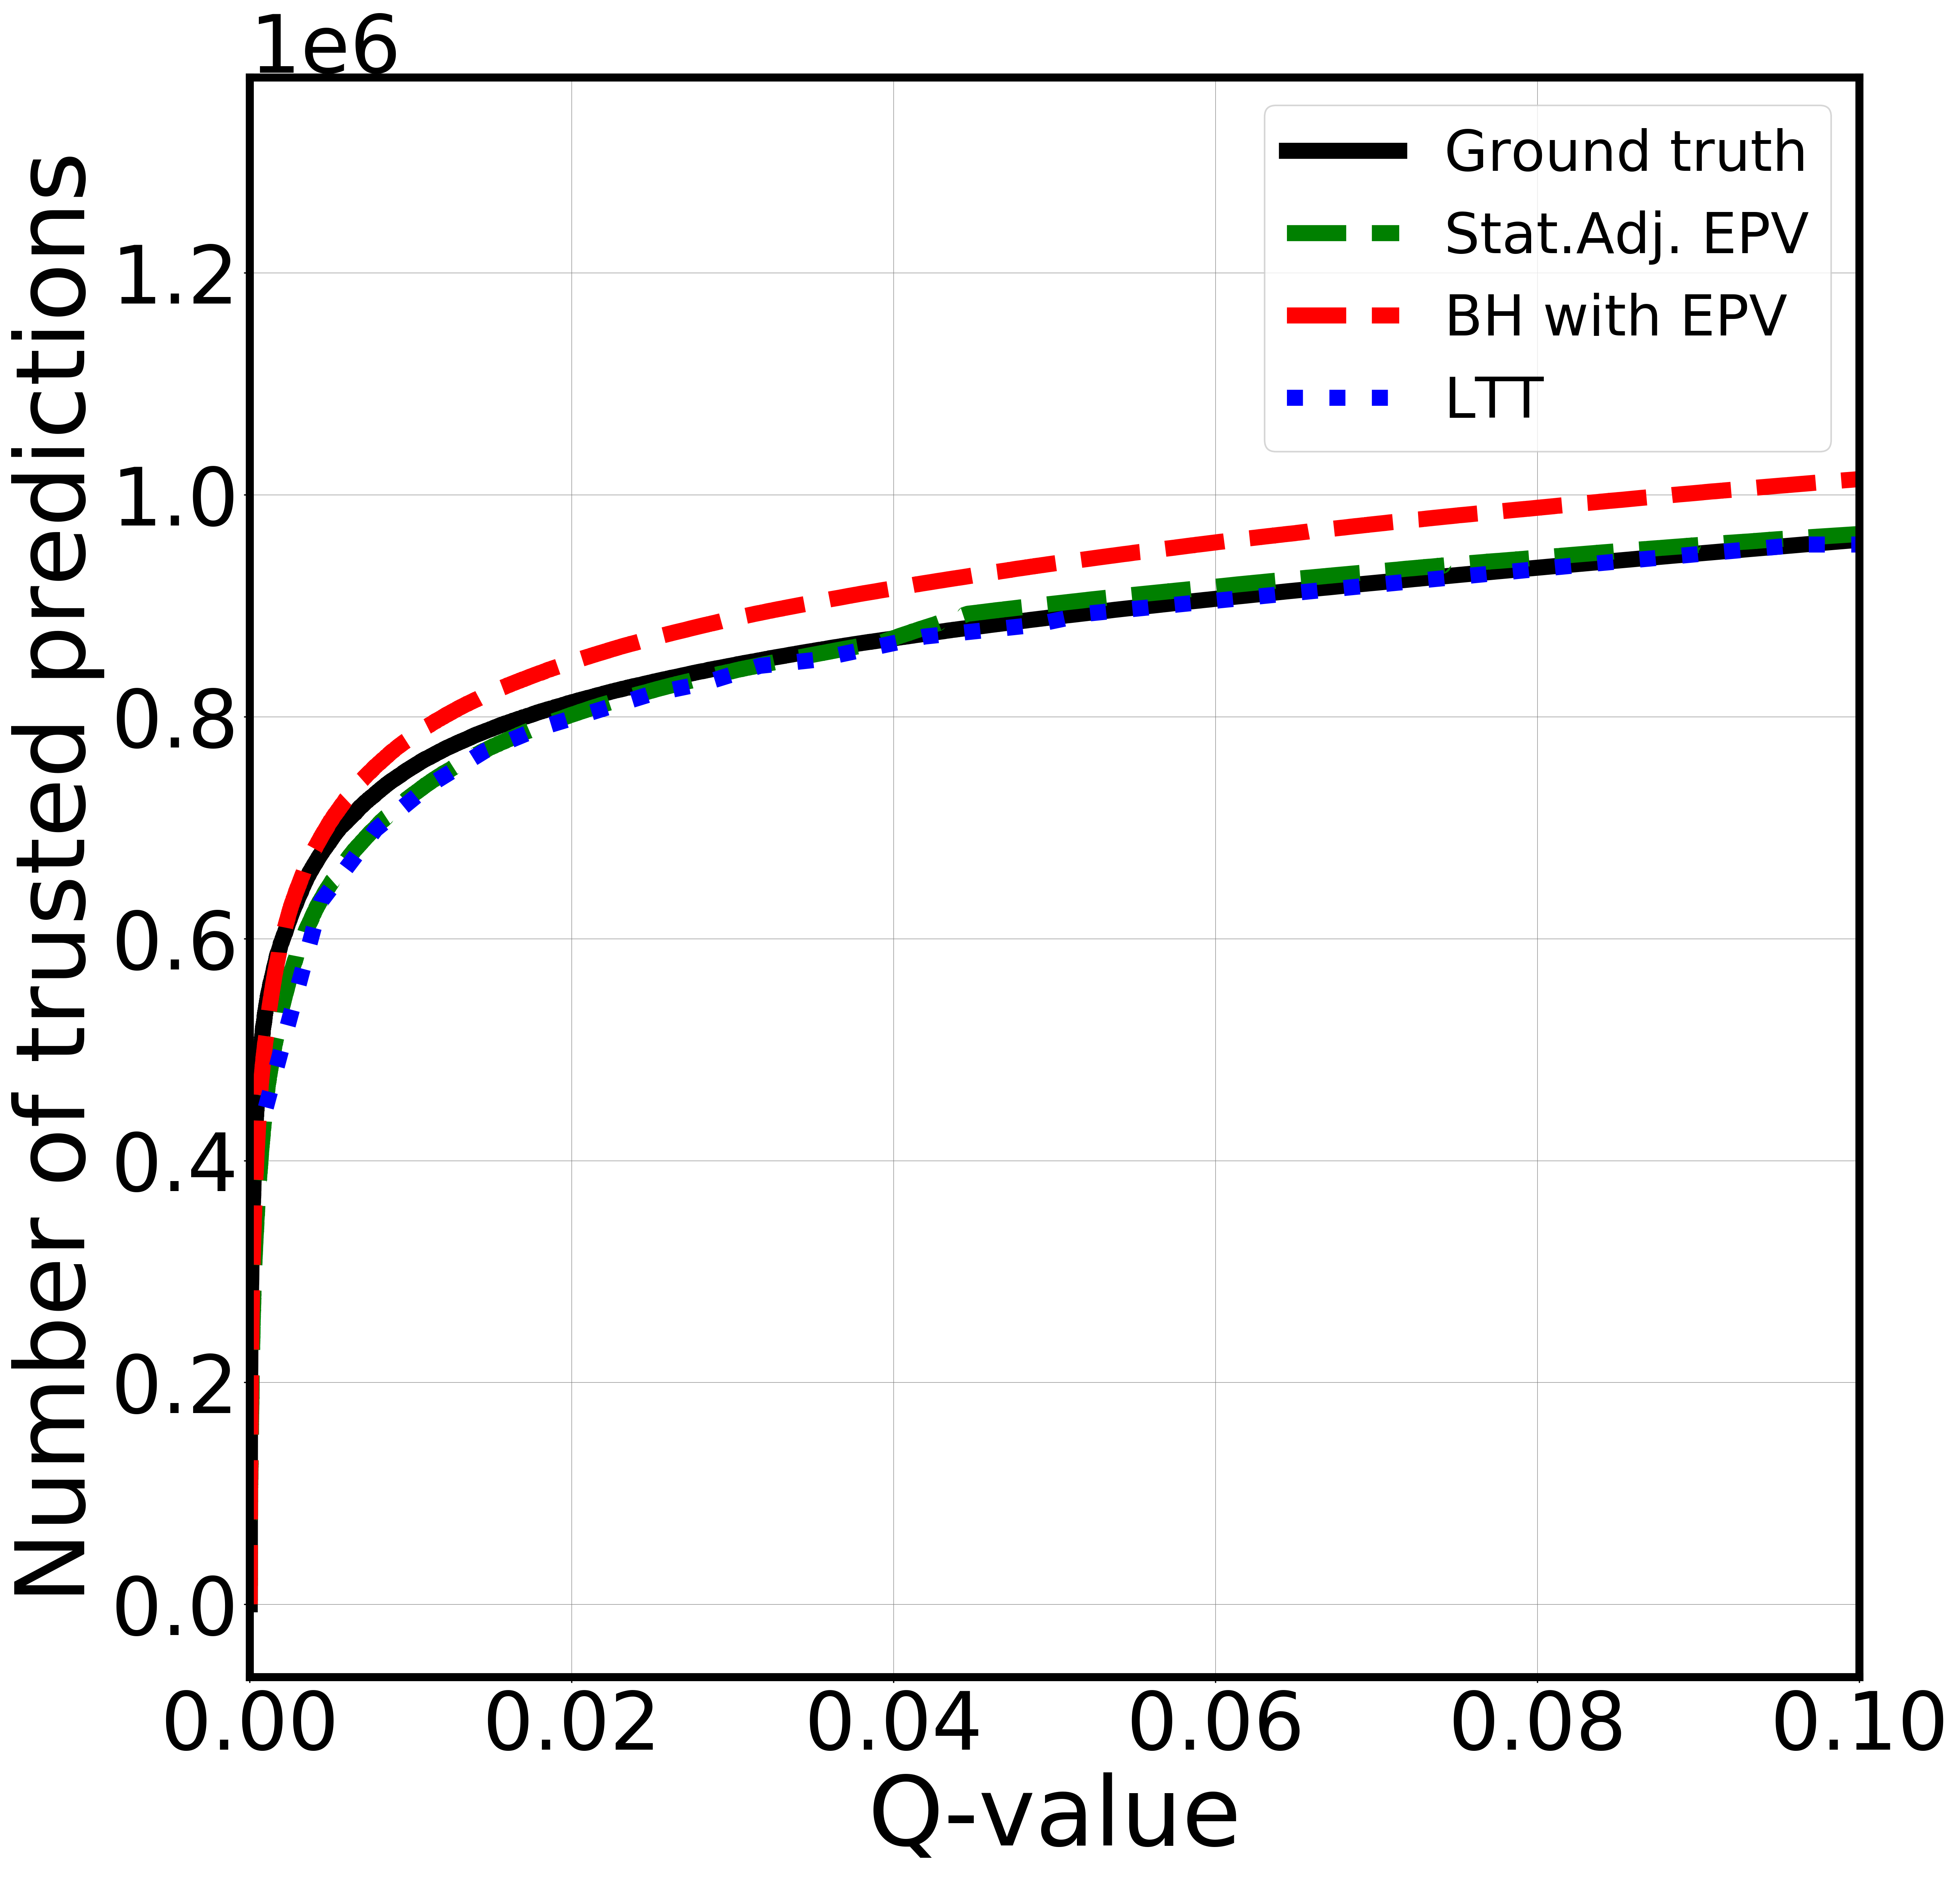
\includegraphics[width=1.7in]{img/cnn_cells_segment_TA_fdr_control_loc.png} & 
		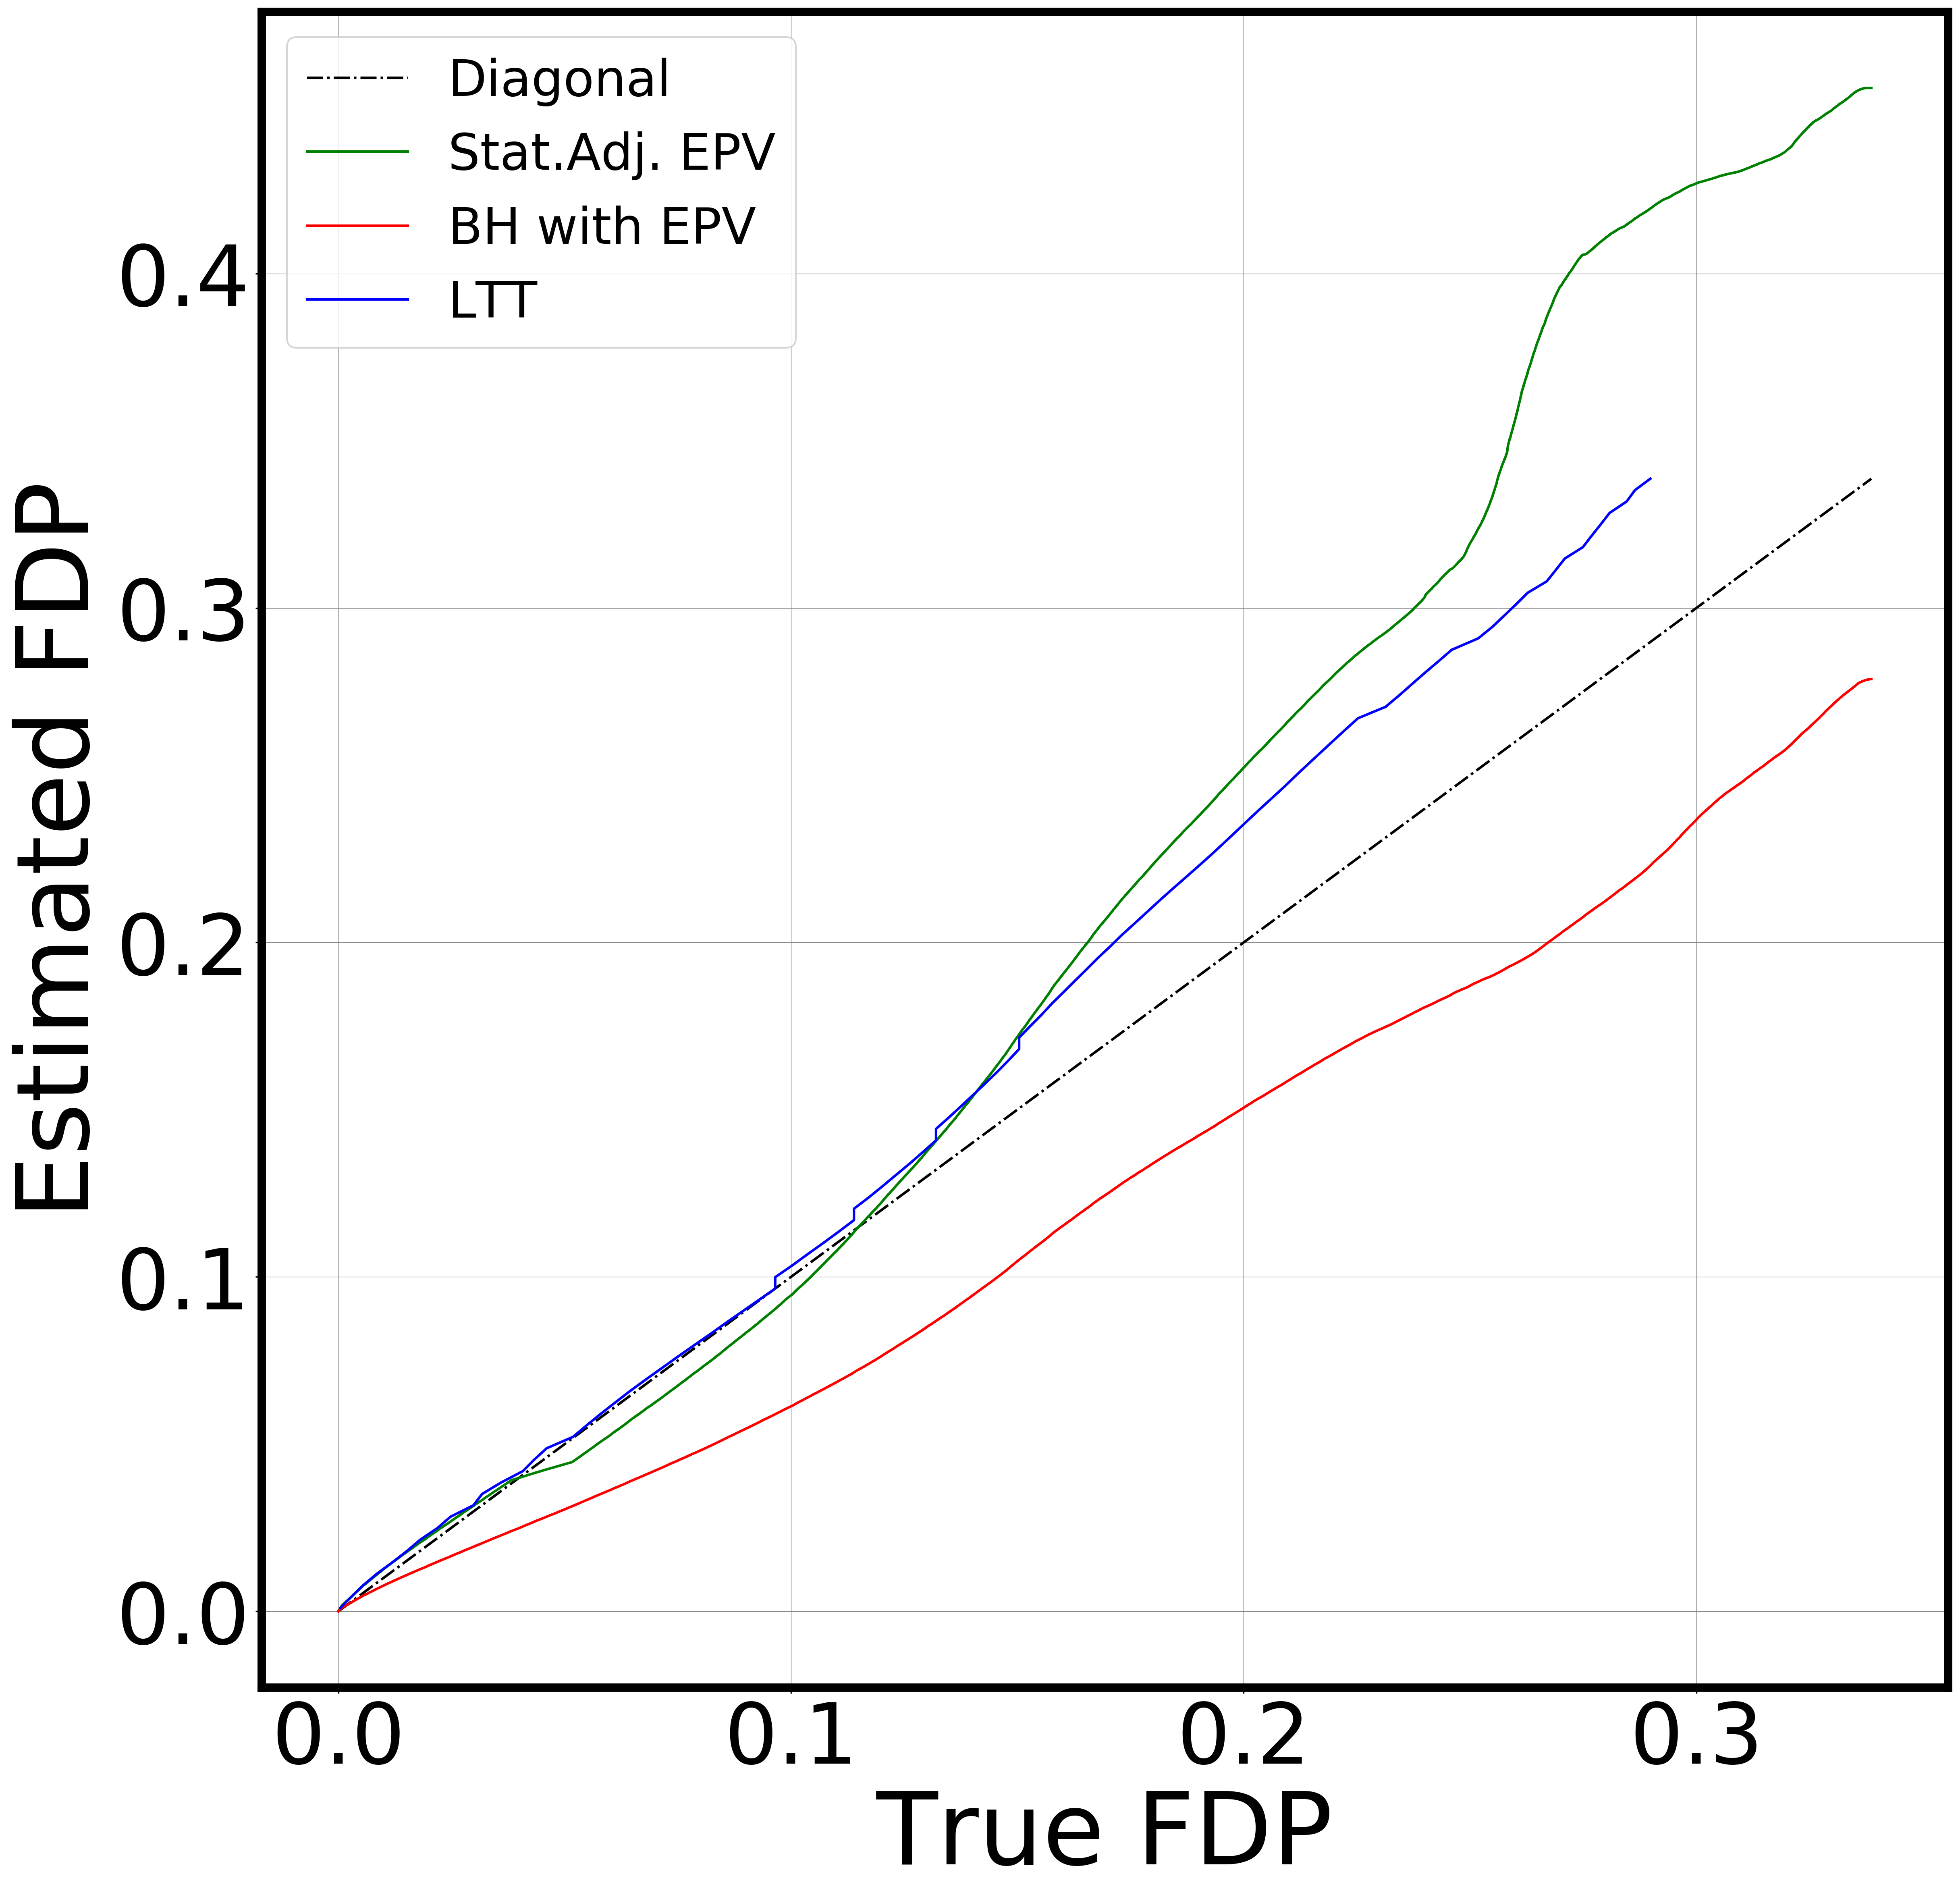
\includegraphics[width=1.7in]{img/cnn_FDPscat_cells_segment_TA.png}\\	
		\multicolumn{4}{l}{\bf (iv) TissueNet with class distribution shift.:}\\		
		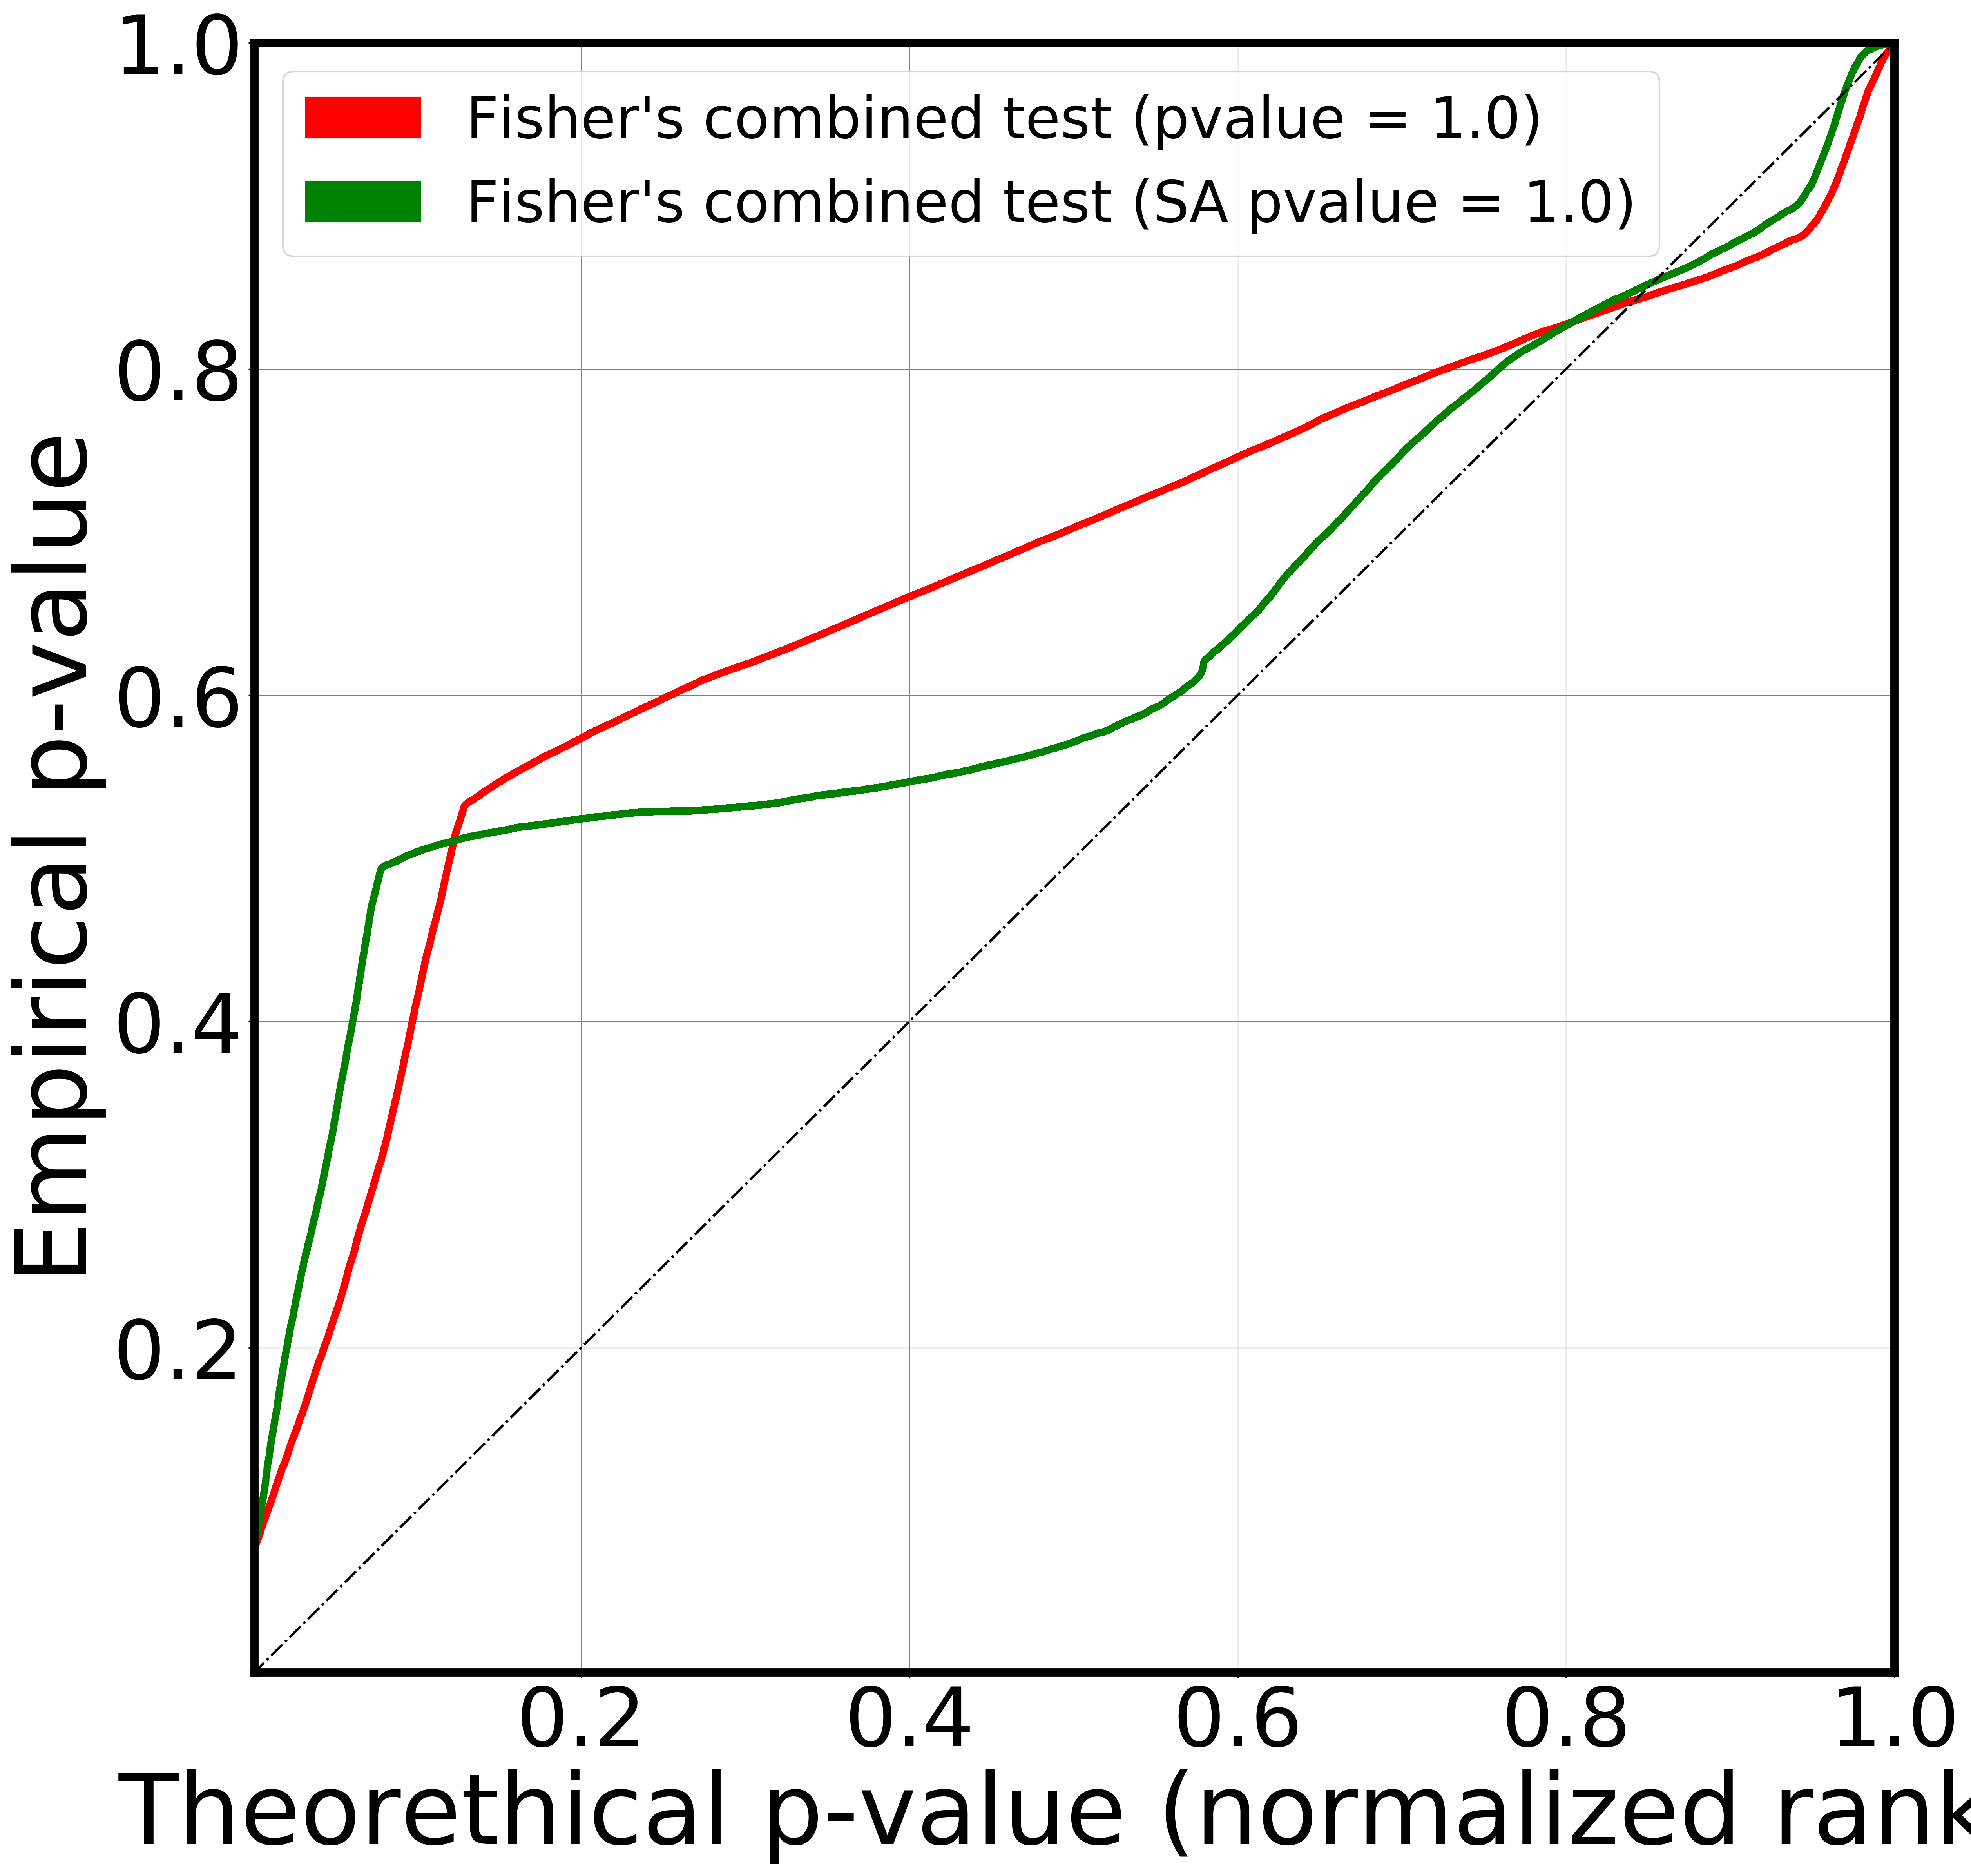
\includegraphics[width=1.7in]{img/cnn_QQ_cells_balanced01.png} &
		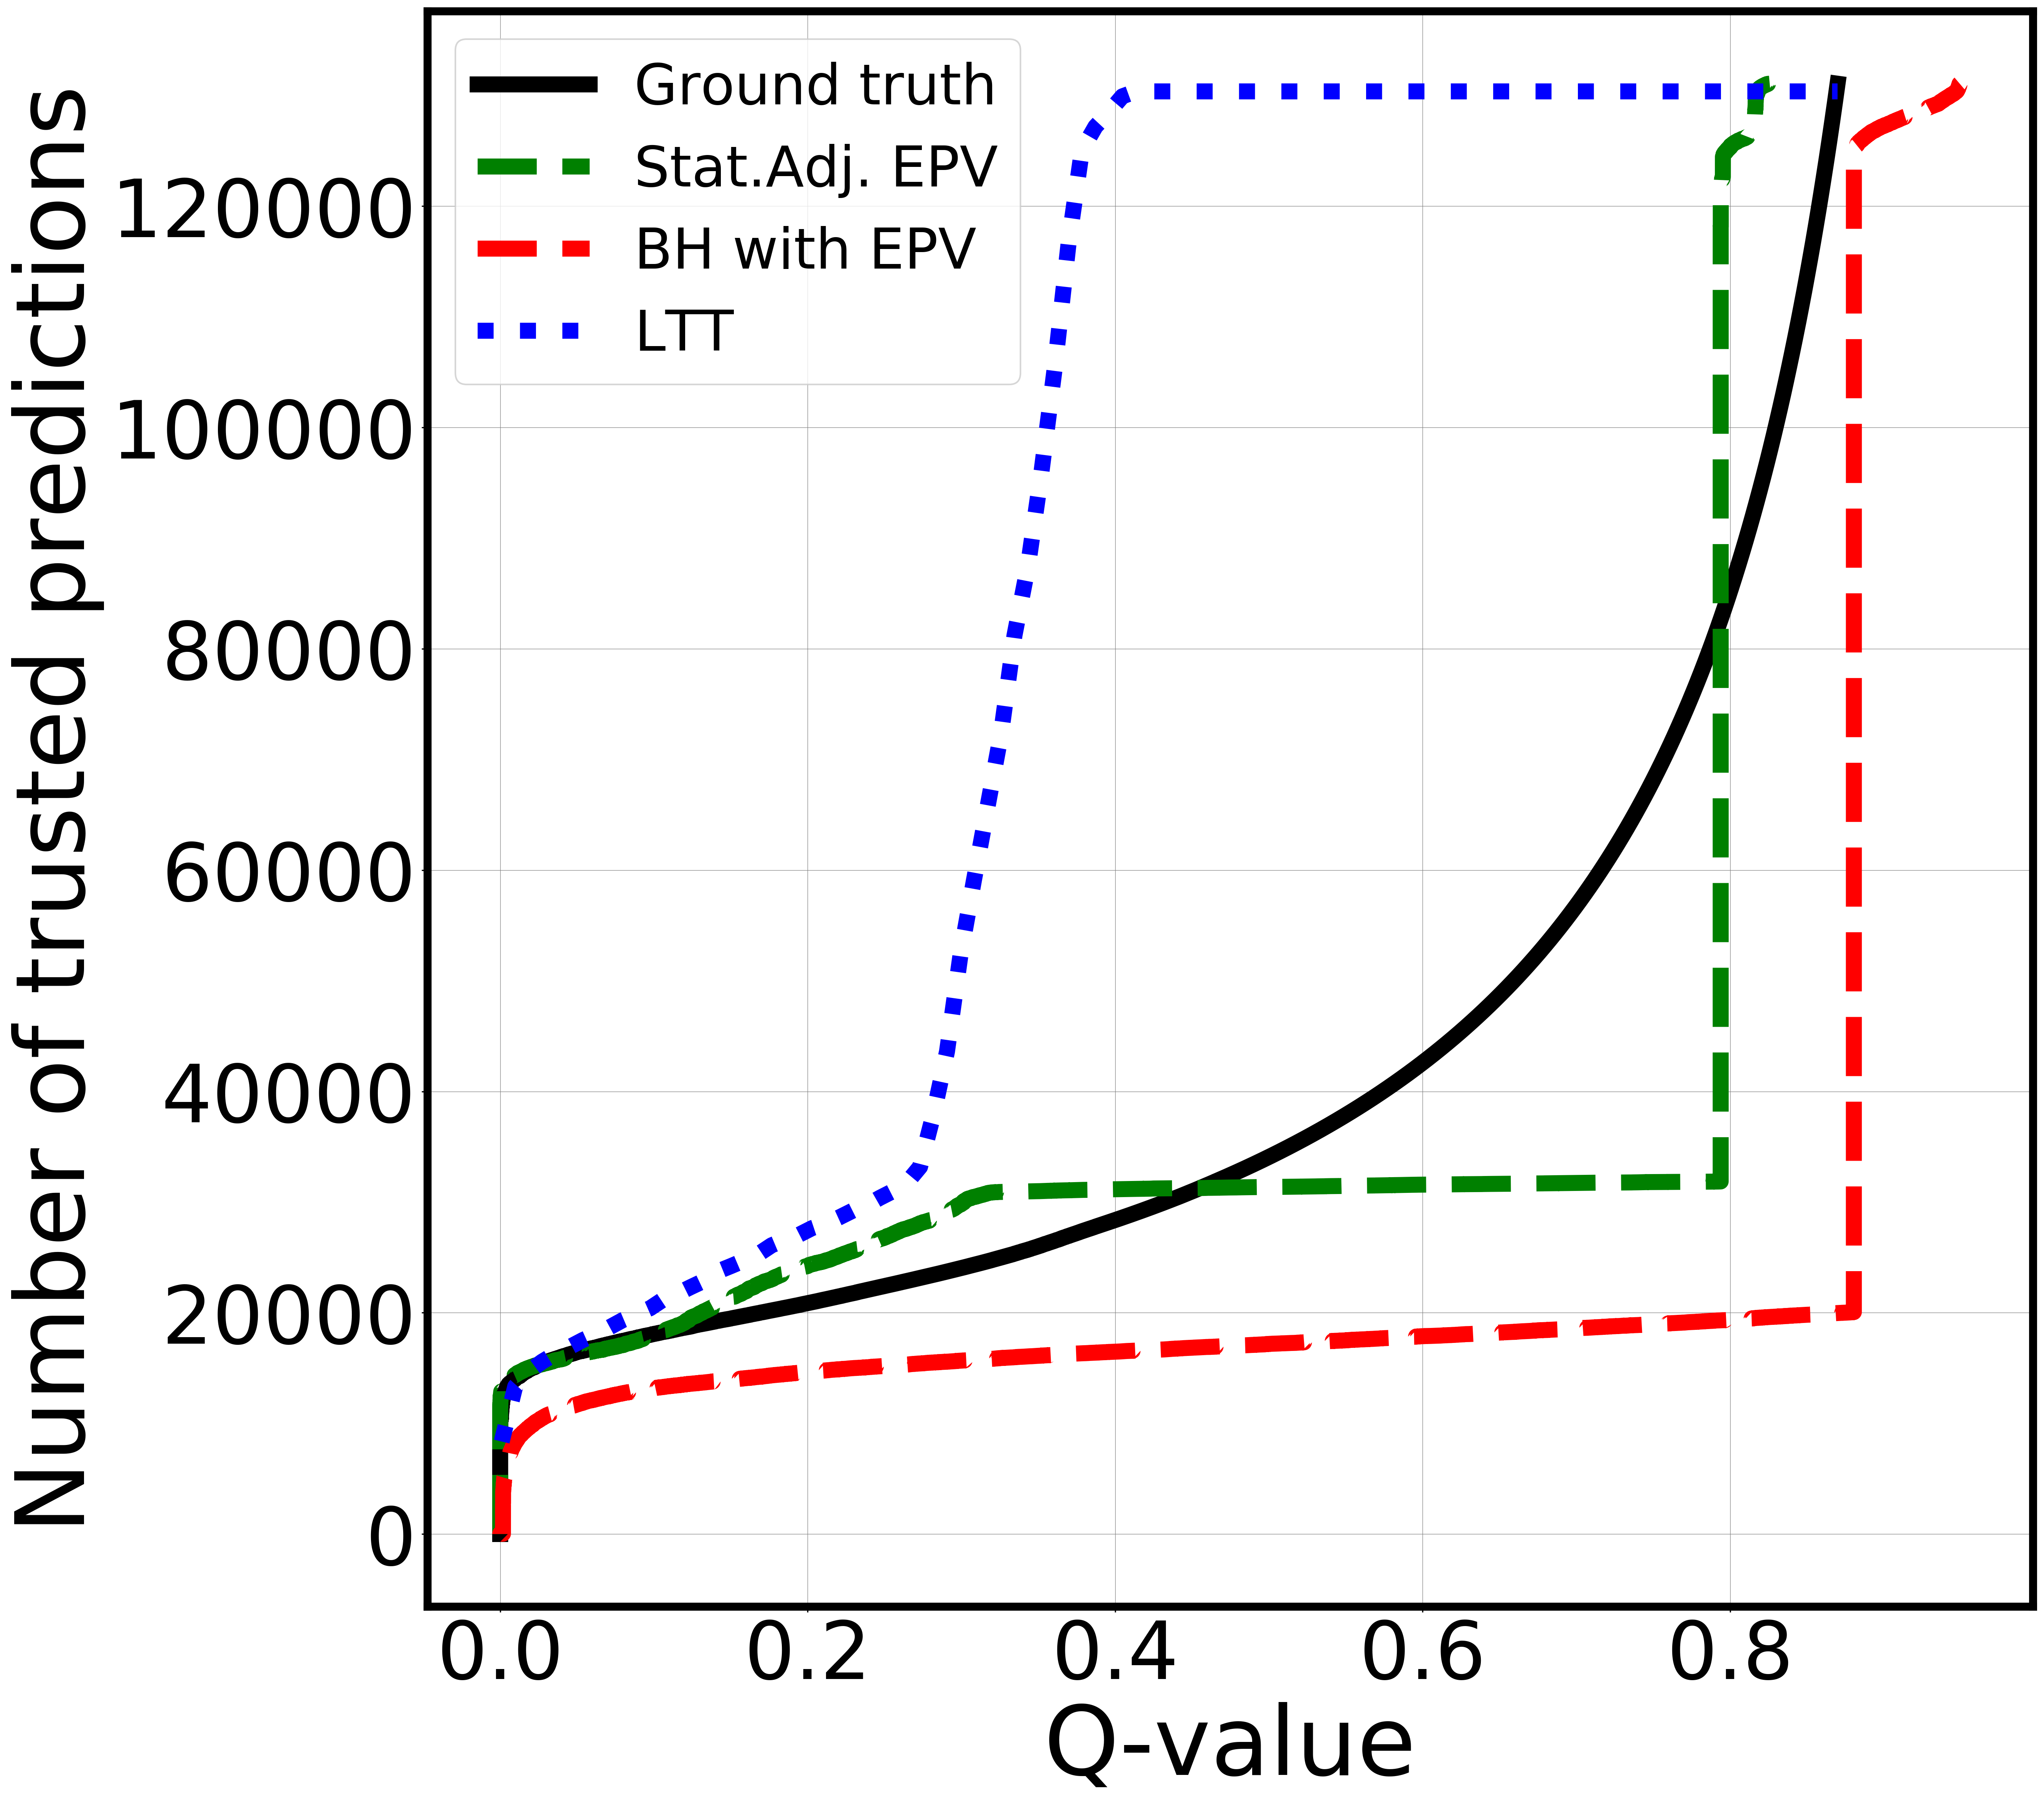
\includegraphics[width=1.7in]{img/cnn_cells_balanced_fdr_control01.png} & 
		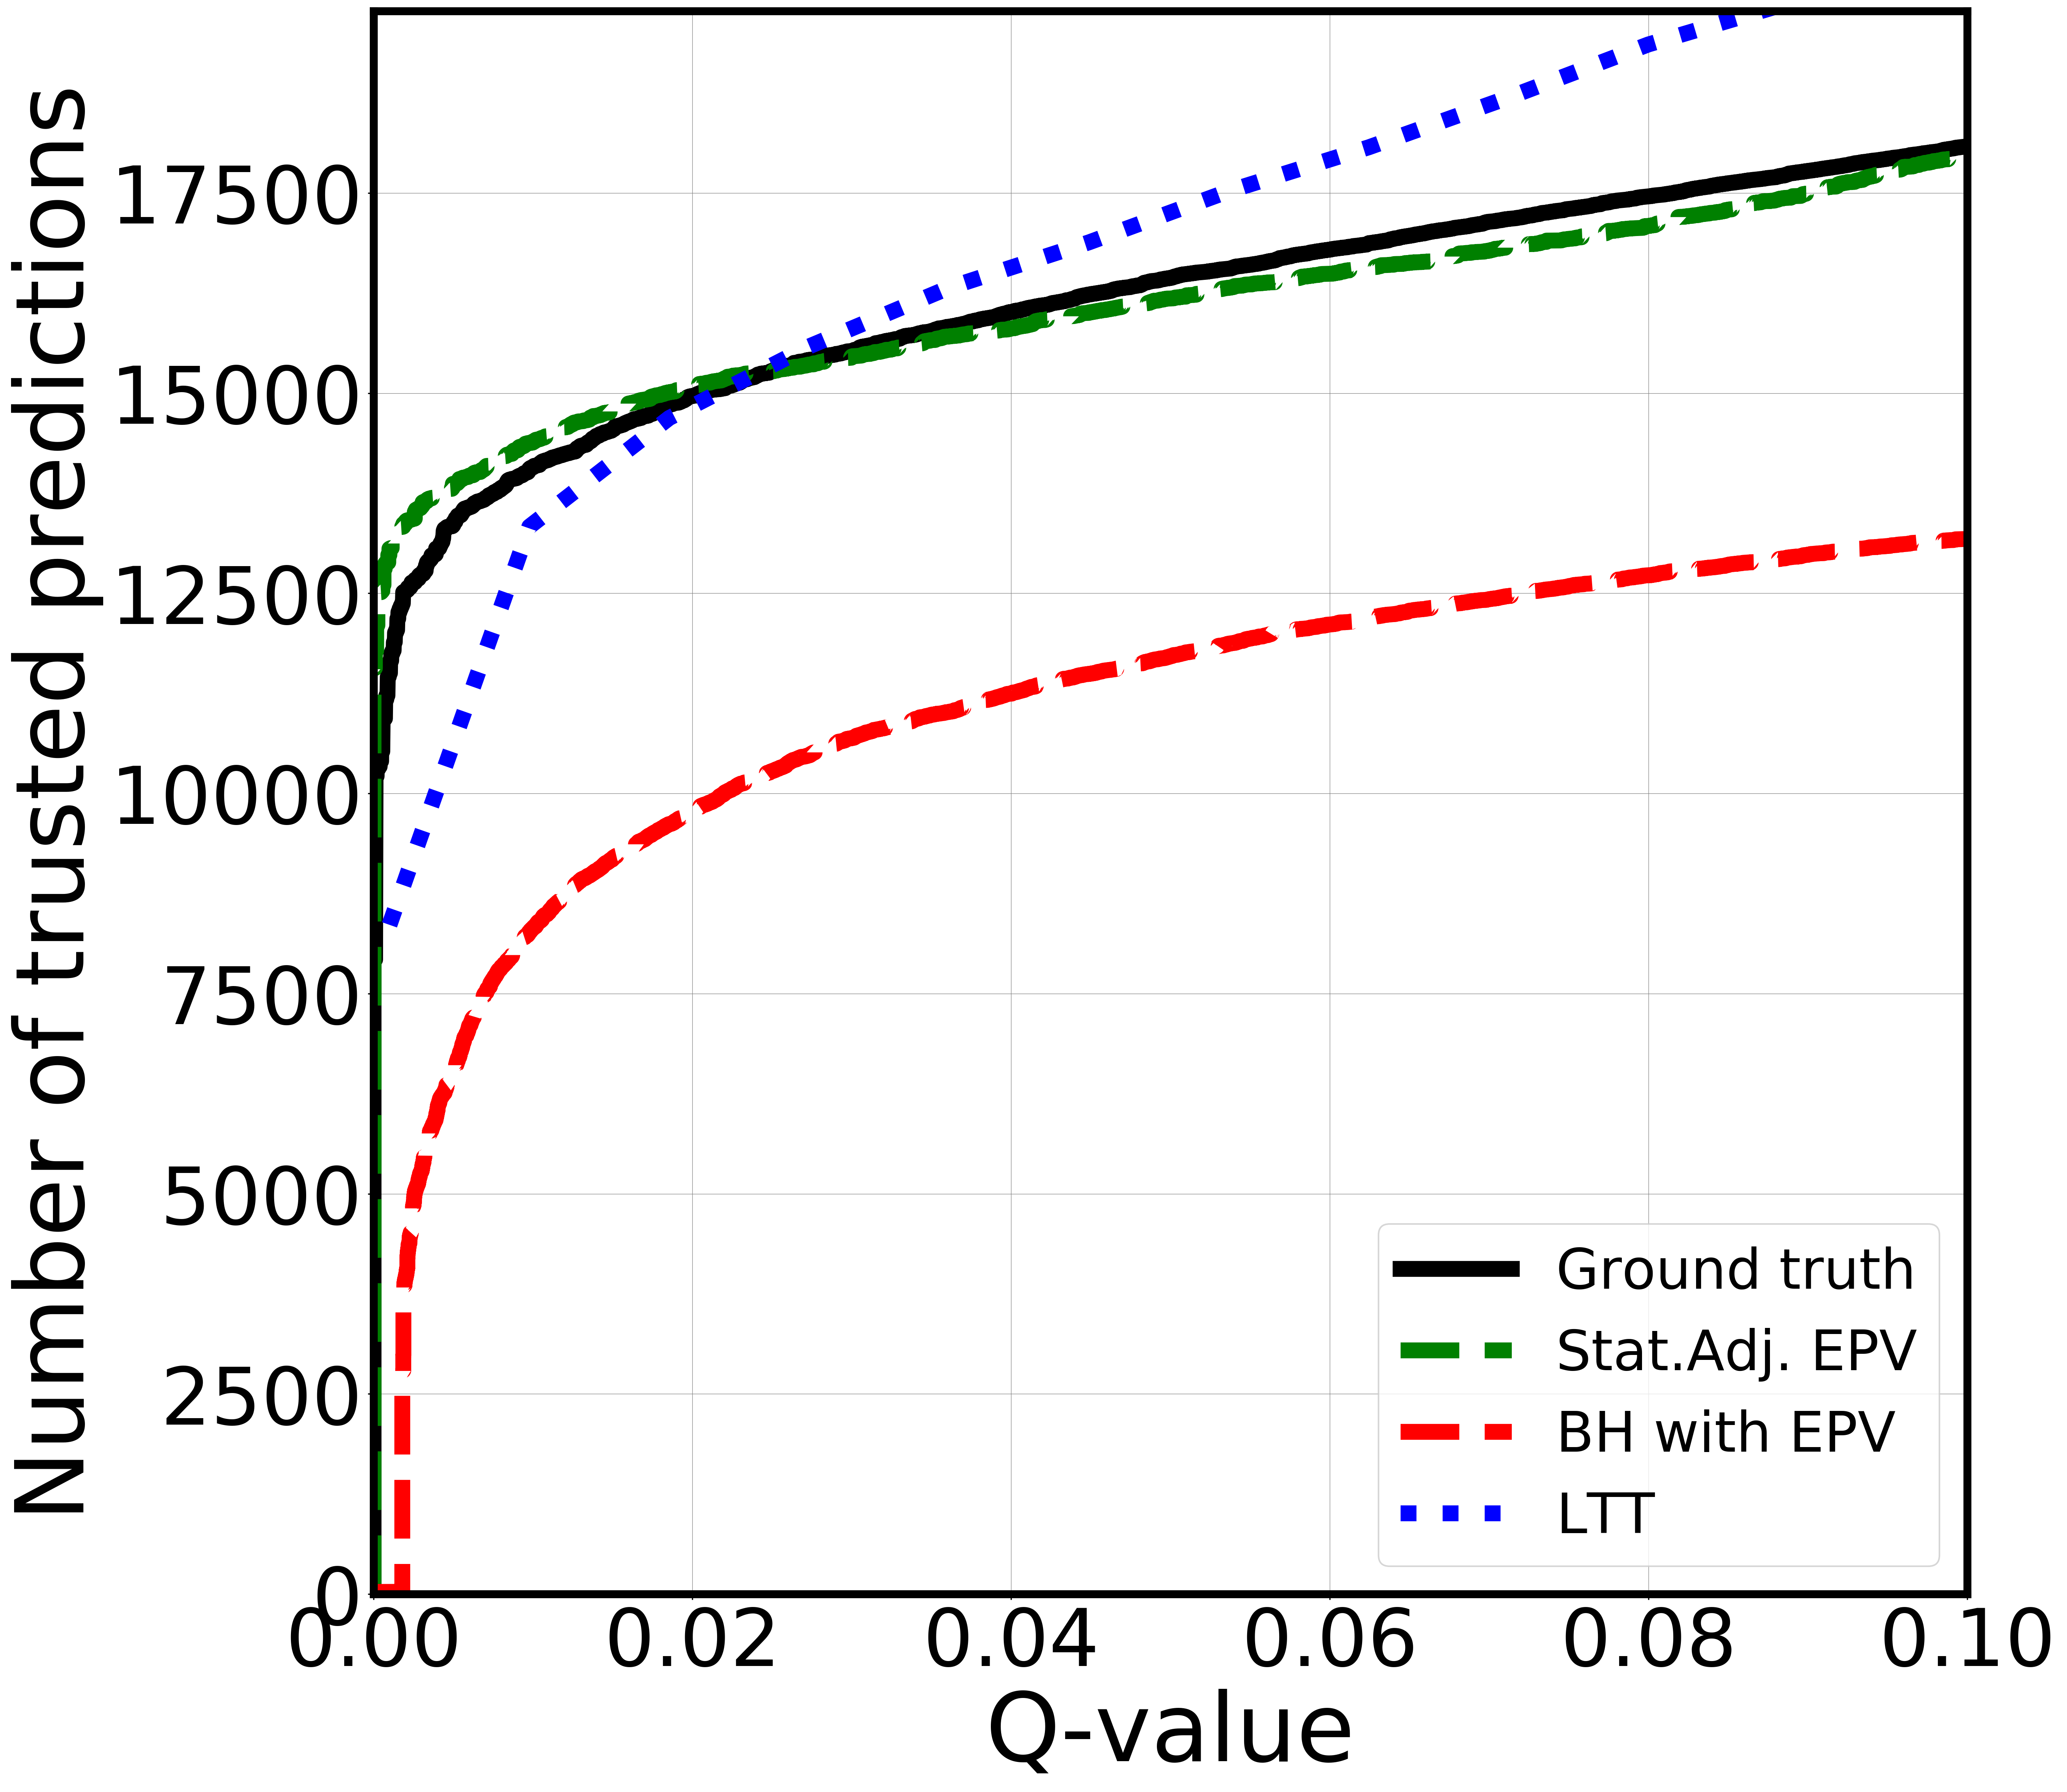
\includegraphics[width=1.7in]{img/cnn_cells_balanced_fdr_control_loc01.png} & 
		\includegraphics[width=1.7in]{img/cnn_FDPscat_cells_balanced01.png}\\			
		A & B & C & D
	\end{tabular}
	\caption{{\bf Performance evaluation of FDR controlling methods.} (A) QQ plot of the EPVs (red dots) and the TNA EPVs (green dots) against the theoretical uniform distribution. The results of the Fisher's combination tests are indicated in the legend. (B) The number of accepted classifications as a function of the Q-values obtained with (i) ground truth (black line), (ii) BH with EPV (red), (iii) BH with TNA EPV (green), and (iv) LTT (blue). (C) Same as (B) but over a critical Q-value range. (D) Deviation of the estimated FDR from the actual FDR obtained with (i) BH with EPV (red line), (ii) BH with EPV and TNA (green line), (iii) LTT (blue line).}
	\label{fig:pcam}
\end{figure} 
\subsection{CheXpert: chest x-ray dataset}

The CheXpert dataset comprises a total of 224,316 radiographs of both frontal and lateral views of the thorax from $\sim$65,000 patients in order to facilitate the automated interpretation of chest X-rays for multi-label classification tasks. We used the deep neural network model, called DenseNet121, from the \texttt{Torchxrayvision} package \cite{cohen2020limits,Cohen2022xrv}, specifically developed for this CheXpert dataset. While CheXpert is of multi-labeled, we turned it to a binary classification in which we treated the Pleural Effusion class as positive and all others as negative. The proportion of the positive class was 27 \% and 23 \% in the training and test datasets. and fine-tuned the DenseNet121 model accordingly, and it achieved 89 \% and 84 \% accuracies on the training and test sets.

We run our evaluation and we found out that all methods: BH with standard EPVs and with TNA EPVs, and the LTT method, provide accurate FDR control. In our opinion, this indicates the absence of any database distribution shits. The also shows that out TNA method does not mess up with the training or test null distributions when there is no data shift.

% This comprehensive corpus encompasses both frontal and lateral views of the thorax. The principal objective of this dataset is to facilitate the automated interpretation of chest X-rays for the task of multi-label classification. It is noteworthy that the dataset is enhanced with uncertainty labels, which provide additional context surrounding the confidence levels of the predictions made by automated systems. Furthermore, the CheXpert dataset includes radiologist-labeled reference standard evaluation sets, which serve as a benchmark for assessing the accuracy and reliability of automated interpretation algorithms in comparison to human expert evaluations. The integration of diverse data types and reference standards positions the CheXpert dataset as a significant resource for advancing research and development in medical imaging and machine learning applications.

%As for the selected model, a DenseNet121, being specifically elaborated for the CheXpert dataset as a part of extensive package called 'Torchxrayvision' \cite{cohen2020limits}\cite{Cohen2022xrv}, was chosen. While it initially was designed to solve a task of multilabel classification among xray images, we further finetuned it for classifying 'Pleural Effusion' only. The proportion of positive class within the training set reached 27\%, insignificantly overwhelming the same number for test - 23\%. Similar situation is seen in context of the measured quality: 89\% accuracy against 84\% for train and test respectively. Therefore, no significant shift of data or class proportion rebalance is identified, which in turn might lead to challenges for those models trained when dealing with real-life applications. For instance, in \cite{joseph_d__viviano__2019} authors elaborate on the issue of poor generalisation abilities of algorithms being trained on a specific dataset of xray images and then tested on another, being a straight consequence of data distribution shifts.

\begin{figure}[h!]
	\centering
	\begin{tabular}{cccc}
 		\includegraphics[width=1.in]{img/chx_1.jpg} &
		\includegraphics[width=1.in]{img/chx_2.jpg} & 
            \includegraphics[width=1.in]{img/chx_3.jpg} &
             \includegraphics[width=1.in]{img/chx_4.jpg}
        \end{tabular}
	\caption{{\bf Instances of CheXpert dataset.}}
	\label{fig:pcam_example}
\end{figure} 


\begin{figure}[h!]
	
	\begin{tabular}{cccc}
		\multicolumn{4}{l}{\bf (i) Standard BCSS dataset:}\\		
%		\includegraphics[width=1.7in]{img/cnn_QQ_pcam.pdf} &
 		&\includegraphics[width=2in]{img/cnn_multi_sa_bcss_fdr_control.pdf} &
		\includegraphics[width=2in]{img/cnn_multi_sa_bcss_fdr_control_loc.pdf} & \\
%		\includegraphics[width=1.7in]{img/cnn_FDPscat_pcam.pdf}\\	
		\multicolumn{4}{l}{\bf (ii) BCSS with class distribution shift.:}\\		
		\multicolumn{4}{l}{\bf (iii) Standard CheXpert dataset:}\\	
		\includegraphics[width=1.7in]{img/cnn_QQ_chx.png} 		&
		\includegraphics[width=1.7in]{img/cnn_chx_fdr_control.png} & 
        \includegraphics[width=1.7in]{img/cnn_chx_fdr_control_loc.png} & 
        \includegraphics[width=1.7in]{img/cnn_FDPscat_chx.png}\\
		A & B & C & D
	\end{tabular}
	\caption{{\bf Performance evaluation of FDR controling methods.} Plot explanation is same as in Figure \ref{fig:pcam}. }
	\label{fig:bcss}
\end{figure} 

\section{Conclusions}

In this study, we investigated the effects of data shift on False Discovery Rate (FDR) control. In our opinion, BH procedure with standard EPVs provide very accurate FDR control in the absence of any data shift. Unfortunately, data shift is rather common in practice, and we demonstrated that standard BH and the LTT methods are quite sensitive even to small data of class distribution shift. In this paper, we presented a simple, but robust method, called Test Null Adjustment (TNA), in order to mitigate the effect of the data shift on FDR control. Our method operates in the space of prediction scores, thereby it is not effected by the course of conditionality problem, which often hinders methods that aim to mitigate data shift in the input feature space. The TNA method consists of two main steps. First, it approximates the null distribution among the scores of the test instances via certain statistics from the distributions of the scores of the training instances. Second, it recalibrates the test scores so that the test and train null distributions would move closer to each other. TNA is fully data-driven, it does not rely on any theoretical assumptions or forms of the data. We have demonstrated in our experimental test with four biomedical datasets that NTA can successfully mitigate the bias caused by data shift; while, leaving the distributions intact in the absence of data shift. We note that, handling data shift in practice is hard, and unfortunately our method does not provide any theoretical guarantee that the FDR control with TNA EPVs becomes accurate, or conservatively or liberally biased without any additional assumptions; hence it is a heuristic in its general form.  

With this study, we also aim to emphasize and popularize the importance of accurate error control in any predictions in the biomedical domain. We have shown that the deviations in the simple QQ plots of the calculated vs. the theoretical p-values can be used to detect data shifts between the training and test data. Moreover, we also hope that the FDR control and plot using q-values will become a standard metric in performance evaluation for prediction systems in the biomedical domain.




%\todo{andrey}{rewrite conclusion, add discussion}
%The original exact p-value (XPV) calculation methods for scoring tandem mass spectrometry data using a dot-product-like scoring function were introduced for low-resolution fragmentation settings almost 15 years ago. Until now, it has remained an open question whether this algorithm can be made suitable for high resolution fragmentation settings. In this article we showed a generalization of the XPV method, termed HR-XPV, which is capable of producing accurate and well calibrated exact p-values for XCorr scores obtained with scoring high resolution MS/MS data. Unfortunately, our solution can be considered rather slow, which raise questions about its practicality. However, we hope that, the ideas in HR-XPV presented might be a significant step toward the development of efficient methods for calibrating exact p-values for high resolution MS/MS data. 

\section*{Author contributions}
\ifdefined\DOUBLEBLINDREVIEW
Omitted for double-blind peer-review.
\else
AKF concieved the idea that accurate empirical p-values would be derived from training data. AB worked out the methods and carried out experiments. AKF and AB wrote the manuscript.
\fi

%\printbibliography	 
%\bibliographystyle{plain}           % Style BST file.
\bibliographystyle{unsrt}           % Style BST file.
\bibliography{bibliography}

\end{document}
